% Options for packages loaded elsewhere
\PassOptionsToPackage{unicode}{hyperref}
\PassOptionsToPackage{hyphens}{url}
\PassOptionsToPackage{dvipsnames,svgnames,x11names}{xcolor}
%
\documentclass[
  letterpaper,
  DIV=11,
  numbers=noendperiod]{scrreprt}

\usepackage{amsmath,amssymb}
\usepackage{iftex}
\ifPDFTeX
  \usepackage[T1]{fontenc}
  \usepackage[utf8]{inputenc}
  \usepackage{textcomp} % provide euro and other symbols
\else % if luatex or xetex
  \usepackage{unicode-math}
  \defaultfontfeatures{Scale=MatchLowercase}
  \defaultfontfeatures[\rmfamily]{Ligatures=TeX,Scale=1}
\fi
\usepackage{lmodern}
\ifPDFTeX\else  
    % xetex/luatex font selection
\fi
% Use upquote if available, for straight quotes in verbatim environments
\IfFileExists{upquote.sty}{\usepackage{upquote}}{}
\IfFileExists{microtype.sty}{% use microtype if available
  \usepackage[]{microtype}
  \UseMicrotypeSet[protrusion]{basicmath} % disable protrusion for tt fonts
}{}
\makeatletter
\@ifundefined{KOMAClassName}{% if non-KOMA class
  \IfFileExists{parskip.sty}{%
    \usepackage{parskip}
  }{% else
    \setlength{\parindent}{0pt}
    \setlength{\parskip}{6pt plus 2pt minus 1pt}}
}{% if KOMA class
  \KOMAoptions{parskip=half}}
\makeatother
\usepackage{xcolor}
\setlength{\emergencystretch}{3em} % prevent overfull lines
\setcounter{secnumdepth}{5}
% Make \paragraph and \subparagraph free-standing
\makeatletter
\ifx\paragraph\undefined\else
  \let\oldparagraph\paragraph
  \renewcommand{\paragraph}{
    \@ifstar
      \xxxParagraphStar
      \xxxParagraphNoStar
  }
  \newcommand{\xxxParagraphStar}[1]{\oldparagraph*{#1}\mbox{}}
  \newcommand{\xxxParagraphNoStar}[1]{\oldparagraph{#1}\mbox{}}
\fi
\ifx\subparagraph\undefined\else
  \let\oldsubparagraph\subparagraph
  \renewcommand{\subparagraph}{
    \@ifstar
      \xxxSubParagraphStar
      \xxxSubParagraphNoStar
  }
  \newcommand{\xxxSubParagraphStar}[1]{\oldsubparagraph*{#1}\mbox{}}
  \newcommand{\xxxSubParagraphNoStar}[1]{\oldsubparagraph{#1}\mbox{}}
\fi
\makeatother

\usepackage{color}
\usepackage{fancyvrb}
\newcommand{\VerbBar}{|}
\newcommand{\VERB}{\Verb[commandchars=\\\{\}]}
\DefineVerbatimEnvironment{Highlighting}{Verbatim}{commandchars=\\\{\}}
% Add ',fontsize=\small' for more characters per line
\usepackage{framed}
\definecolor{shadecolor}{RGB}{241,243,245}
\newenvironment{Shaded}{\begin{snugshade}}{\end{snugshade}}
\newcommand{\AlertTok}[1]{\textcolor[rgb]{0.68,0.00,0.00}{#1}}
\newcommand{\AnnotationTok}[1]{\textcolor[rgb]{0.37,0.37,0.37}{#1}}
\newcommand{\AttributeTok}[1]{\textcolor[rgb]{0.40,0.45,0.13}{#1}}
\newcommand{\BaseNTok}[1]{\textcolor[rgb]{0.68,0.00,0.00}{#1}}
\newcommand{\BuiltInTok}[1]{\textcolor[rgb]{0.00,0.23,0.31}{#1}}
\newcommand{\CharTok}[1]{\textcolor[rgb]{0.13,0.47,0.30}{#1}}
\newcommand{\CommentTok}[1]{\textcolor[rgb]{0.37,0.37,0.37}{#1}}
\newcommand{\CommentVarTok}[1]{\textcolor[rgb]{0.37,0.37,0.37}{\textit{#1}}}
\newcommand{\ConstantTok}[1]{\textcolor[rgb]{0.56,0.35,0.01}{#1}}
\newcommand{\ControlFlowTok}[1]{\textcolor[rgb]{0.00,0.23,0.31}{\textbf{#1}}}
\newcommand{\DataTypeTok}[1]{\textcolor[rgb]{0.68,0.00,0.00}{#1}}
\newcommand{\DecValTok}[1]{\textcolor[rgb]{0.68,0.00,0.00}{#1}}
\newcommand{\DocumentationTok}[1]{\textcolor[rgb]{0.37,0.37,0.37}{\textit{#1}}}
\newcommand{\ErrorTok}[1]{\textcolor[rgb]{0.68,0.00,0.00}{#1}}
\newcommand{\ExtensionTok}[1]{\textcolor[rgb]{0.00,0.23,0.31}{#1}}
\newcommand{\FloatTok}[1]{\textcolor[rgb]{0.68,0.00,0.00}{#1}}
\newcommand{\FunctionTok}[1]{\textcolor[rgb]{0.28,0.35,0.67}{#1}}
\newcommand{\ImportTok}[1]{\textcolor[rgb]{0.00,0.46,0.62}{#1}}
\newcommand{\InformationTok}[1]{\textcolor[rgb]{0.37,0.37,0.37}{#1}}
\newcommand{\KeywordTok}[1]{\textcolor[rgb]{0.00,0.23,0.31}{\textbf{#1}}}
\newcommand{\NormalTok}[1]{\textcolor[rgb]{0.00,0.23,0.31}{#1}}
\newcommand{\OperatorTok}[1]{\textcolor[rgb]{0.37,0.37,0.37}{#1}}
\newcommand{\OtherTok}[1]{\textcolor[rgb]{0.00,0.23,0.31}{#1}}
\newcommand{\PreprocessorTok}[1]{\textcolor[rgb]{0.68,0.00,0.00}{#1}}
\newcommand{\RegionMarkerTok}[1]{\textcolor[rgb]{0.00,0.23,0.31}{#1}}
\newcommand{\SpecialCharTok}[1]{\textcolor[rgb]{0.37,0.37,0.37}{#1}}
\newcommand{\SpecialStringTok}[1]{\textcolor[rgb]{0.13,0.47,0.30}{#1}}
\newcommand{\StringTok}[1]{\textcolor[rgb]{0.13,0.47,0.30}{#1}}
\newcommand{\VariableTok}[1]{\textcolor[rgb]{0.07,0.07,0.07}{#1}}
\newcommand{\VerbatimStringTok}[1]{\textcolor[rgb]{0.13,0.47,0.30}{#1}}
\newcommand{\WarningTok}[1]{\textcolor[rgb]{0.37,0.37,0.37}{\textit{#1}}}

\providecommand{\tightlist}{%
  \setlength{\itemsep}{0pt}\setlength{\parskip}{0pt}}\usepackage{longtable,booktabs,array}
\usepackage{calc} % for calculating minipage widths
% Correct order of tables after \paragraph or \subparagraph
\usepackage{etoolbox}
\makeatletter
\patchcmd\longtable{\par}{\if@noskipsec\mbox{}\fi\par}{}{}
\makeatother
% Allow footnotes in longtable head/foot
\IfFileExists{footnotehyper.sty}{\usepackage{footnotehyper}}{\usepackage{footnote}}
\makesavenoteenv{longtable}
\usepackage{graphicx}
\makeatletter
\newsavebox\pandoc@box
\newcommand*\pandocbounded[1]{% scales image to fit in text height/width
  \sbox\pandoc@box{#1}%
  \Gscale@div\@tempa{\textheight}{\dimexpr\ht\pandoc@box+\dp\pandoc@box\relax}%
  \Gscale@div\@tempb{\linewidth}{\wd\pandoc@box}%
  \ifdim\@tempb\p@<\@tempa\p@\let\@tempa\@tempb\fi% select the smaller of both
  \ifdim\@tempa\p@<\p@\scalebox{\@tempa}{\usebox\pandoc@box}%
  \else\usebox{\pandoc@box}%
  \fi%
}
% Set default figure placement to htbp
\def\fps@figure{htbp}
\makeatother

\KOMAoption{captions}{tableheading}
\makeatletter
\@ifpackageloaded{tcolorbox}{}{\usepackage[skins,breakable]{tcolorbox}}
\@ifpackageloaded{fontawesome5}{}{\usepackage{fontawesome5}}
\definecolor{quarto-callout-color}{HTML}{909090}
\definecolor{quarto-callout-note-color}{HTML}{0758E5}
\definecolor{quarto-callout-important-color}{HTML}{CC1914}
\definecolor{quarto-callout-warning-color}{HTML}{EB9113}
\definecolor{quarto-callout-tip-color}{HTML}{00A047}
\definecolor{quarto-callout-caution-color}{HTML}{FC5300}
\definecolor{quarto-callout-color-frame}{HTML}{acacac}
\definecolor{quarto-callout-note-color-frame}{HTML}{4582ec}
\definecolor{quarto-callout-important-color-frame}{HTML}{d9534f}
\definecolor{quarto-callout-warning-color-frame}{HTML}{f0ad4e}
\definecolor{quarto-callout-tip-color-frame}{HTML}{02b875}
\definecolor{quarto-callout-caution-color-frame}{HTML}{fd7e14}
\makeatother
\makeatletter
\@ifpackageloaded{bookmark}{}{\usepackage{bookmark}}
\makeatother
\makeatletter
\@ifpackageloaded{caption}{}{\usepackage{caption}}
\AtBeginDocument{%
\ifdefined\contentsname
  \renewcommand*\contentsname{Table of contents}
\else
  \newcommand\contentsname{Table of contents}
\fi
\ifdefined\listfigurename
  \renewcommand*\listfigurename{List of Figures}
\else
  \newcommand\listfigurename{List of Figures}
\fi
\ifdefined\listtablename
  \renewcommand*\listtablename{List of Tables}
\else
  \newcommand\listtablename{List of Tables}
\fi
\ifdefined\figurename
  \renewcommand*\figurename{Figure}
\else
  \newcommand\figurename{Figure}
\fi
\ifdefined\tablename
  \renewcommand*\tablename{Table}
\else
  \newcommand\tablename{Table}
\fi
}
\@ifpackageloaded{float}{}{\usepackage{float}}
\floatstyle{ruled}
\@ifundefined{c@chapter}{\newfloat{codelisting}{h}{lop}}{\newfloat{codelisting}{h}{lop}[chapter]}
\floatname{codelisting}{Listing}
\newcommand*\listoflistings{\listof{codelisting}{List of Listings}}
\makeatother
\makeatletter
\makeatother
\makeatletter
\@ifpackageloaded{caption}{}{\usepackage{caption}}
\@ifpackageloaded{subcaption}{}{\usepackage{subcaption}}
\makeatother

\usepackage{bookmark}

\IfFileExists{xurl.sty}{\usepackage{xurl}}{} % add URL line breaks if available
\urlstyle{same} % disable monospaced font for URLs
\hypersetup{
  pdftitle={Pani Simulator},
  pdfauthor={Rishabh Sharma},
  colorlinks=true,
  linkcolor={blue},
  filecolor={Maroon},
  citecolor={Blue},
  urlcolor={Blue},
  pdfcreator={LaTeX via pandoc}}


\title{Pani Simulator}
\author{Rishabh Sharma}
\date{2025-05-07}

\begin{document}
\maketitle

\renewcommand*\contentsname{Table of contents}
{
\hypersetup{linkcolor=}
\setcounter{tocdepth}{2}
\tableofcontents
}

\bookmarksetup{startatroot}

\chapter*{Pani Simulator}\label{pani-simulator}
\addcontentsline{toc}{chapter}{Pani Simulator}

\markboth{Pani Simulator}{Pani Simulator}

Pani (which means \(\textit{water}\) in Hindi) is a high fidelity marine
vessel simulator. It is built in a manner such that minimum backend
edits are required by the user and the simulator can be both configured
and run in an intuitive lightweight GUI application which runs on the
web. An attempt to make it as ``Microsoft's Flight Simualtor'' but for
marine vessels has been made.

The simulator can be used to configure a new marine vessel, simulate
sensors such as DVL, IMU, LiDAR and Camera, and control the vessel
either via teleop input or custom files for autonomous tasks. The
simulator supports multiple agents which is useful for swarm autonomy
tasks or to develop better collision avoidance algorithms.

The project has been made open source to allow for further development
of this simulator and add additional features to make it more versatile.

\section*{Overview}\label{overview}
\addcontentsline{toc}{section}{Overview}

\markright{Overview}

The Simulator is majorly divided into two parts:

\begin{itemize}
\tightlist
\item
  Vessel Configurator
\item
  Vessel Simulation
\end{itemize}

The Vessel Configurator is what allows you to configure a new marine
vessel. You can load a FBX Geometry file, select individual components
such as control surfaces, thrusters, sensors and configure their
parameters via the interactive GUI. If you like a more geeky experience,
you can edit the input files manually as well. There are also options to
enter the non-linear hydrodynamics coefficients for the vessel (which we
plan to integrate with our in-house system identification algorithm, in
future), set vessel geometry parameters and specify initial conditions.
This is also where you will setup the simulation parameters such as
time, time-step, geofence, GPS datum and physical constants (gravity,
density etc). It also supports the output from our in-house
hydrodynamics program \textit{HyDRA}, which gives the added mass
coefficients and wave hydrodynamics of the vessel. Once you are done
with the vessel configuration, the program auto generates the input
files required for the simulation to run.

\begin{figure}[H]

{\centering \pandocbounded{\includegraphics[keepaspectratio]{./images/vesselConfigurator.png}}

}

\caption{Vessel Configurator}

\end{figure}%

The Vessel Simulation is where the actual simulation takes place. It
follows the dynamics as per the parameters you set in the Vessel
Configurator. This is where you can also custom code your control and
guidance algorithms which will publish the required data in ROS2 to make
the vessel run. Currently the sensors are simulated with added noise
whose outputs you can see in the ROS2 terminal, or from the GUI. We soon
plan to add modelling for the simulator with real world physics.

\begin{figure}[H]

{\centering \pandocbounded{\includegraphics[keepaspectratio]{./images/simulation2.png}}

}

\caption{Way-point trackingSimulation Visualization}

\end{figure}%

\section*{Key Features}\label{key-features}
\addcontentsline{toc}{section}{Key Features}

\markright{Key Features}

\begin{itemize}
\tightlist
\item
  \textbf{Realistic Physics}: Follows dyanmics modelling as defined by
  Fossen's
  \textit{Handbook of Marine Craft Hydrodynamics and Motion Control}
\item
  \textbf{Modular Architecture}: Easy integration of custom vessel
  models, sensors, and controllers
\item
  \textbf{ROS2 Integration}: Native support for Robot Operating System 2
  (ROS2) for distributed robotics applications
\item
  \textbf{Web Application}: Lightweight web application for configuring
  and running the simulation
\item
  \textbf{Multiple Agents}: Simulate multiple vessels in the same
  environment
\end{itemize}

\section*{How to Use This
Documentation}\label{how-to-use-this-documentation}
\addcontentsline{toc}{section}{How to Use This Documentation}

\markright{How to Use This Documentation}

Navigate through the sections using the sidebar. The documentation
discusses the Setup, theory on the Kinematics and Dynamics used in the
simulator, the coordinate systems used for various components (control
surfaces, thrusters, sensors and Body centre), the python simulator
backend and how to use the Panisim vessel configurator and the Panisim
vessel simulator.

\bookmarksetup{startatroot}

\chapter*{Setup}\label{setup}
\addcontentsline{toc}{chapter}{Setup}

\markboth{Setup}{Setup}

\section*{Prerequisites}\label{prerequisites}
\addcontentsline{toc}{section}{Prerequisites}

\markright{Prerequisites}

\begin{itemize}
\tightlist
\item
  Git installed on your system
\item
  Docker installed on your system
\item
  Basic understanding of terminal commands
\item
  Python version 3.10 or higher
\end{itemize}

\section*{Cloning the Repository}\label{cloning-the-repository}
\addcontentsline{toc}{section}{Cloning the Repository}

\markright{Cloning the Repository}

\begin{enumerate}
\def\labelenumi{\arabic{enumi}.}
\item
  Open a terminal window
\item
  Clone the repository using the following command:

\begin{Shaded}
\begin{Highlighting}[]
\FunctionTok{git}\NormalTok{ clone https://github.com/MarineAutonomy/makara.git}
\end{Highlighting}
\end{Shaded}
\item
  Navigate to the cloned repository:

\begin{Shaded}
\begin{Highlighting}[]
\BuiltInTok{cd}\NormalTok{ makara}
\end{Highlighting}
\end{Shaded}
\item
  Switch to the mavymini branch:

\begin{Shaded}
\begin{Highlighting}[]
\FunctionTok{git}\NormalTok{ checkout mavymini}
\end{Highlighting}
\end{Shaded}
\end{enumerate}

\section*{Building the Docker Image}\label{building-the-docker-image}
\addcontentsline{toc}{section}{Building the Docker Image}

\markright{Building the Docker Image}

Before running the simulator, you need to build the Docker image:

\begin{enumerate}
\def\labelenumi{\arabic{enumi}.}
\item
  Ensure you're in the root directory of the cloned repository
\item
  Build the Docker image by executing:

\begin{Shaded}
\begin{Highlighting}[]
\ExtensionTok{./ros2\_devdocker.sh}
\end{Highlighting}
\end{Shaded}
\item
  Wait for the build process to complete (this may take several minutes
  depending on your internet connection and system performance)
\end{enumerate}

\section*{Troubleshooting}\label{troubleshooting}
\addcontentsline{toc}{section}{Troubleshooting}

\markright{Troubleshooting}

\begin{itemize}
\tightlist
\item
  \textbf{Docker issues}: Ensure Docker is installed and running on your
  system
\item
  \textbf{Permission issues}: If you encounter permission errors when
  running scripts, try prefixing the commands with \texttt{sudo}
\end{itemize}

\bookmarksetup{startatroot}

\chapter*{Quickstart}\label{quickstart}
\addcontentsline{toc}{chapter}{Quickstart}

\markboth{Quickstart}{Quickstart}

After building the Docker image, you can start the simulator:

\begin{enumerate}
\def\labelenumi{\arabic{enumi}.}
\item
  From the root directory of the repository, run the following script in
  your terminal:

\begin{Shaded}
\begin{Highlighting}[]
\ExtensionTok{./ros2\_simulator.sh}
\end{Highlighting}
\end{Shaded}
\item
  Once the simulator starts, it will display the ROS2 topics available
  in the terminal. You should see an output similar to this:

\begin{Shaded}
\begin{Highlighting}[]
\NormalTok{   ==================================================}
\NormalTok{   🚀 ROS2 Simulation Started Successfully!}
\NormalTok{   ==================================================}

\NormalTok{📡 Available ROS2 Topics:}
\NormalTok{{-}{-}{-}{-}{-}{-}{-}{-}{-}{-}{-}{-}{-}{-}{-}{-}{-}{-}{-}{-}{-}{-}{-}{-}{-}{-}{-}{-}{-}{-}}
\NormalTok{/parameter\_events}
\NormalTok{/rosout}
\NormalTok{/sookshma\_00/Rudder\_1/encoder}
\NormalTok{/sookshma\_00/actuator\_cmd}
\NormalTok{/sookshma\_00/imu/data}
\NormalTok{/sookshma\_00/odometry}
\NormalTok{/sookshma\_00/odometry\_sim}
\NormalTok{/sookshma\_00/uwb}
\NormalTok{/sookshma\_00/vessel\_state}
\NormalTok{/sookshma\_00/vessel\_states\_ekf}
\NormalTok{/sookshma\_00/waypoints}

\NormalTok{🔍 View Topic Data:}
\NormalTok{{-}{-}{-}{-}{-}{-}{-}{-}{-}{-}{-}{-}{-}{-}{-}{-}{-}{-}{-}{-}{-}{-}{-}{-}{-}{-}{-}{-}{-}{-}}
\NormalTok{1. Open a new terminal:}
\NormalTok{    docker exec {-}it panisim bash}

\NormalTok{2. Subscribe to a topic:}
\NormalTok{    ros2 topic echo \textless{}topic\_name\textgreater{}}

\NormalTok{📝 Example:}
\NormalTok{    ros2 topic echo /vessel\_0/odometry\_sim}

\NormalTok{==================================================}
\end{Highlighting}
\end{Shaded}

  To inspect the data published on these topics, follow these steps:

  \begin{enumerate}
  \def\labelenumii{\alph{enumii}.}
  \item
    Open a new terminal window.
  \item
    Enter the Docker container by executing the following command in a
    new terminal:
  \end{enumerate}

\begin{Shaded}
\begin{Highlighting}[]
\ExtensionTok{docker}\NormalTok{ exec }\AttributeTok{{-}it}\NormalTok{ panisim bash}
\end{Highlighting}
\end{Shaded}

  \begin{enumerate}
  \def\labelenumii{\alph{enumii}.}
  \setcounter{enumii}{2}
  \tightlist
  \item
    Subscribe to a specific topic using the \texttt{ros2\ topic\ echo}
    command. Replace \texttt{\textless{}topic\_name\textgreater{}} with
    the actual topic you want to inspect.
  \end{enumerate}

\begin{Shaded}
\begin{Highlighting}[]
\ExtensionTok{ros2}\NormalTok{ topic echo }\OperatorTok{\textless{}}\NormalTok{topic\_name}\OperatorTok{\textgreater{}}
\end{Highlighting}
\end{Shaded}

  For example, to view the odometry data for \texttt{mavymini\_00}, you
  would use:

\begin{Shaded}
\begin{Highlighting}[]
\ExtensionTok{ros2}\NormalTok{ topic echo /sookshma\_00/odometry\_sim}
\end{Highlighting}
\end{Shaded}
\end{enumerate}

\begin{tcolorbox}[enhanced jigsaw, colback=white, toptitle=1mm, colframe=quarto-callout-note-color-frame, rightrule=.15mm, breakable, title=\textcolor{quarto-callout-note-color}{\faInfo}\hspace{0.5em}{Note}, toprule=.15mm, opacitybacktitle=0.6, opacityback=0, coltitle=black, leftrule=.75mm, colbacktitle=quarto-callout-note-color!10!white, arc=.35mm, titlerule=0mm, bottomtitle=1mm, bottomrule=.15mm, left=2mm]

The specific topic names may vary depending on the agents activated in
your \texttt{/inputs/simulation\_input.yml} configuration file.

\end{tcolorbox}

Currently, the example vessel is configure with an initial velocity of
0.5m/s. (You can change this by editing the
\texttt{/inputs/simulation\_input.yml} file.)

A Web-based visualization GUI would have started automatically. You can
access it by opening a new browser tab and navigating to
\texttt{http://localhost:8000}.

\begin{figure}[H]

{\centering \pandocbounded{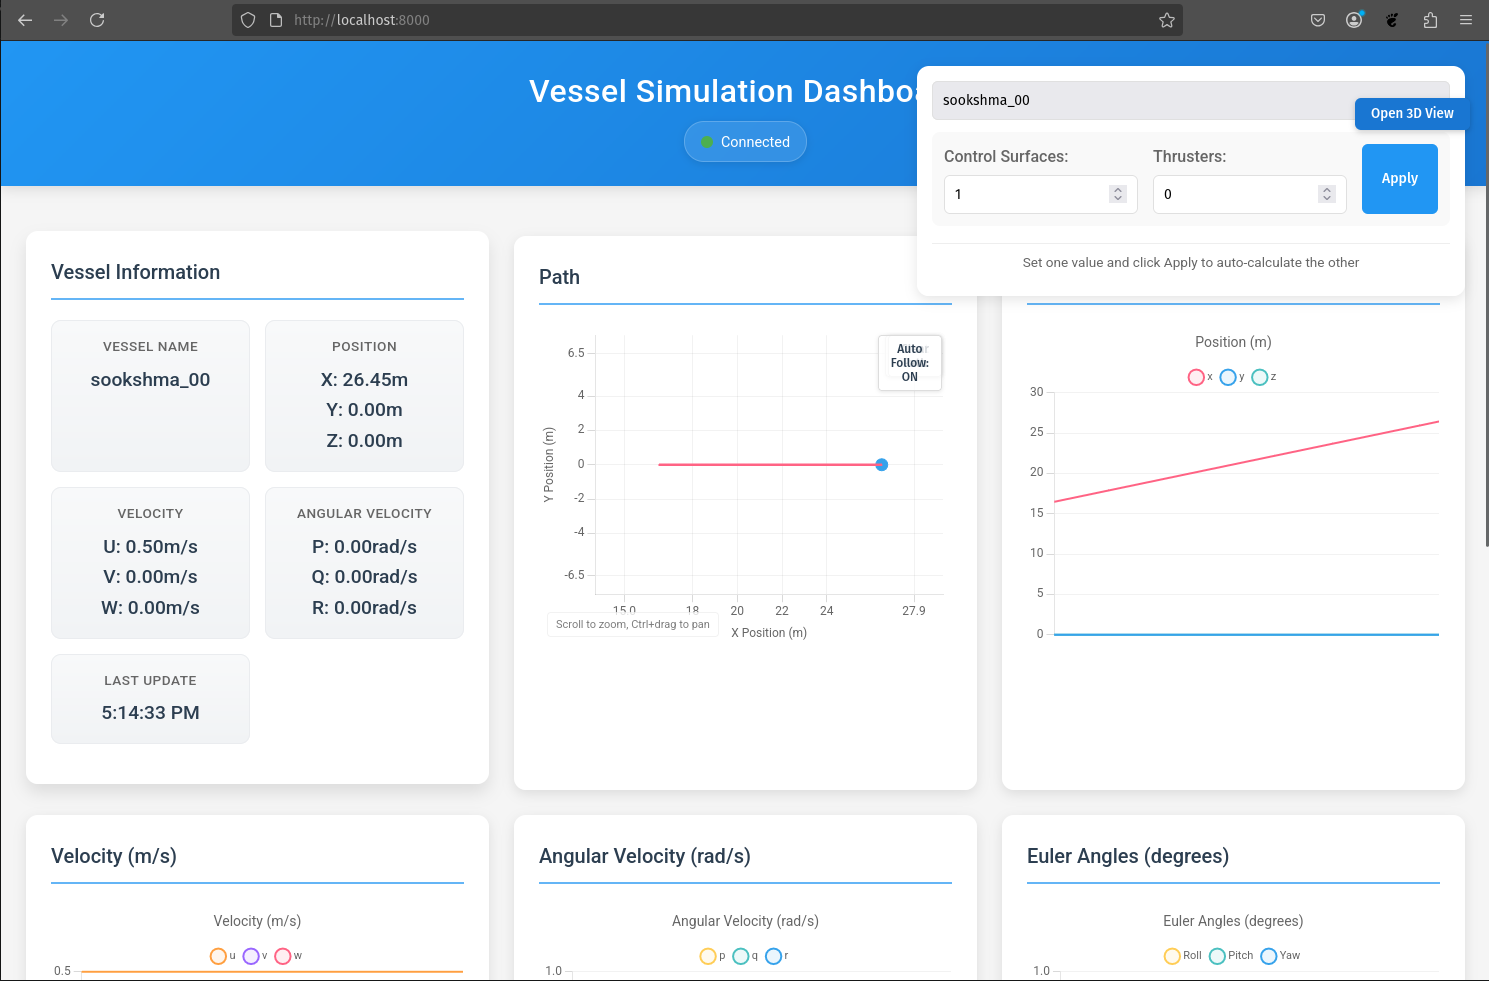
\includegraphics[keepaspectratio]{rawFiles/../images/simVis.png}}

}

\caption{Web-based visualization GUI}

\end{figure}%

This visualization GUI shows you the current state of the vessel,
including its position, velocity, orientation and actuator data.

You can also see the 6 DOF of the vessel via the ``Open 3D View''
button. A new window will appear showing you a box shaped vessel with
its position and orientation in the simulation.

\begin{figure}[H]

{\centering \pandocbounded{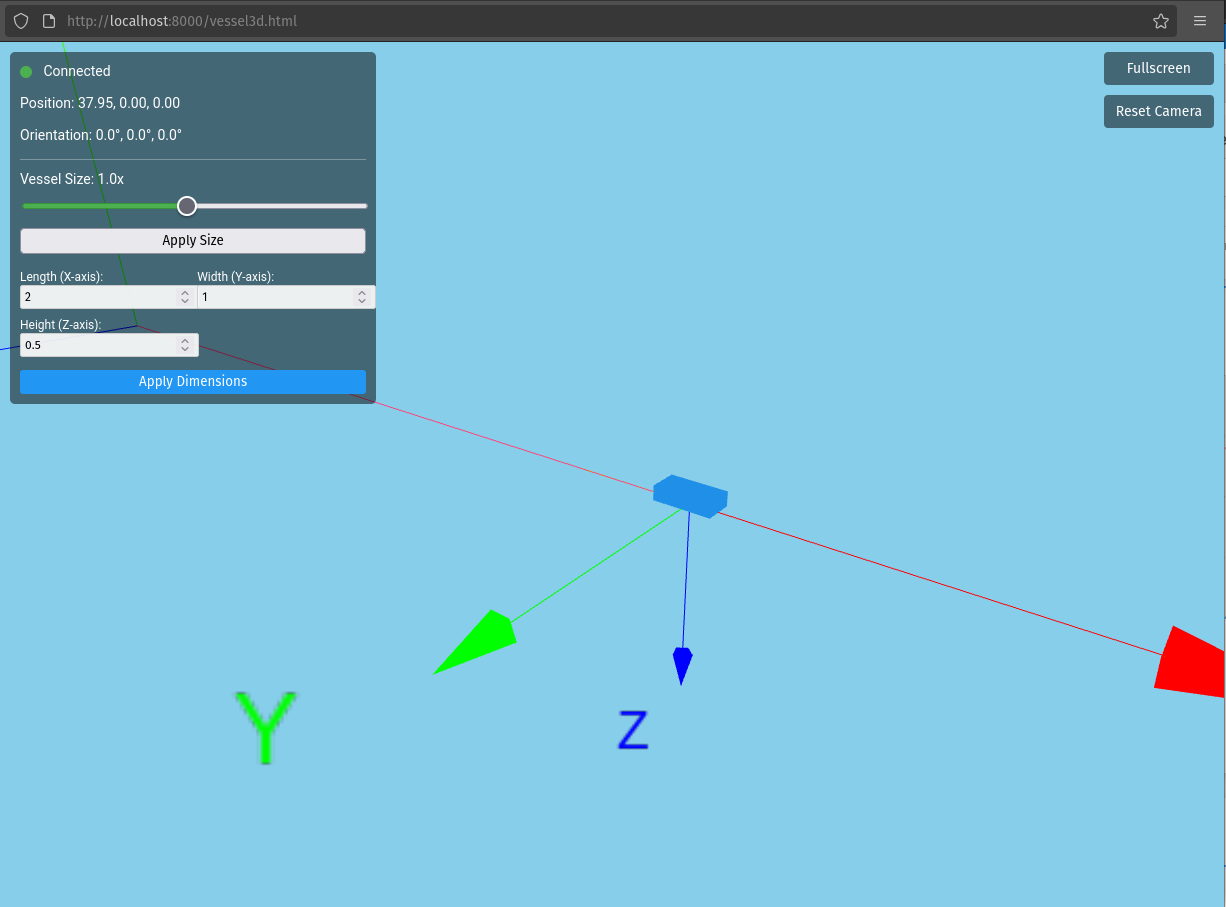
\includegraphics[keepaspectratio]{rawFiles/../images/threeDvis.png}}

}

\caption{3D View}

\end{figure}%

And that's it! The simulation is up and running and now you can start
any other ROS nodes to command the vessel actuators, perform Extended
Kalman Filtering, or anything else you want. We will be covering a
waypoint tracking example to show you how you can write your own ROS2
nodes to control your vessel.

\bookmarksetup{startatroot}

\chapter*{Kinematics}\label{kinematics}
\addcontentsline{toc}{chapter}{Kinematics}

\markboth{Kinematics}{Kinematics}

\section*{Overview}\label{overview-1}
\addcontentsline{toc}{section}{Overview}

\markright{Overview}

The Kinematics module (\texttt{module\_kinematics.py}) provides a
comprehensive set of mathematical functions for handling coordinate
transformations, rotation representations, and kinematic calculations
essential for marine vehicle simulation.

\begin{tcolorbox}[enhanced jigsaw, colback=white, toptitle=1mm, colframe=quarto-callout-tip-color-frame, rightrule=.15mm, breakable, title=\textcolor{quarto-callout-tip-color}{\faLightbulb}\hspace{0.5em}{Tip}, toprule=.15mm, opacitybacktitle=0.6, opacityback=0, coltitle=black, leftrule=.75mm, colbacktitle=quarto-callout-tip-color!10!white, arc=.35mm, titlerule=0mm, bottomtitle=1mm, bottomrule=.15mm, left=2mm]

This module serves as the mathematical foundation for all spatial
transformations in the simulator.

\end{tcolorbox}

\section*{Coordinate Frames}\label{coordinate-frames}
\addcontentsline{toc}{section}{Coordinate Frames}

\markright{Coordinate Frames}

The simulator utilizes several key coordinate frames:

\begin{enumerate}
\def\labelenumi{\arabic{enumi}.}
\tightlist
\item
  \textbf{Earth Centered Inertial (ECI) frame \{i\}}: An inertial frame
  with its origin at the Earth's center. It does not rotate with the
  Earth's rotation.
\item
  \textbf{Earth Centered Earth Fixed (ECEF) frame \{e\}}: Rotates with
  the Earth. Its origin is at the Earth's center. The x-axis passes
  through the intersection of the prime meridian and the equator, the
  z-axis aligns with the Earth's rotation axis, and the y-axis completes
  the right-handed system.
\item
  \textbf{North-East-Down (NED) frame \{n\}}: A local tangent frame
  fixed to a point on the Earth's surface (or a reference point). The
  x-axis points North, the y-axis points East, and the z-axis points
  Down, perpendicular to the Earth's ellipsoid surface. This is the
  primary navigation frame.
\item
  \textbf{Body frame \{b\}}: An orthogonal frame fixed to the vehicle.
  The x-axis points forward, the y-axis points right (starboard), and
  the z-axis points down.
\end{enumerate}

\section*{Function Categories}\label{function-categories}
\addcontentsline{toc}{section}{Function Categories}

\markright{Function Categories}

\subsection*{Rotation Representation
Conversions}\label{rotation-representation-conversions}
\addcontentsline{toc}{subsection}{Rotation Representation Conversions}

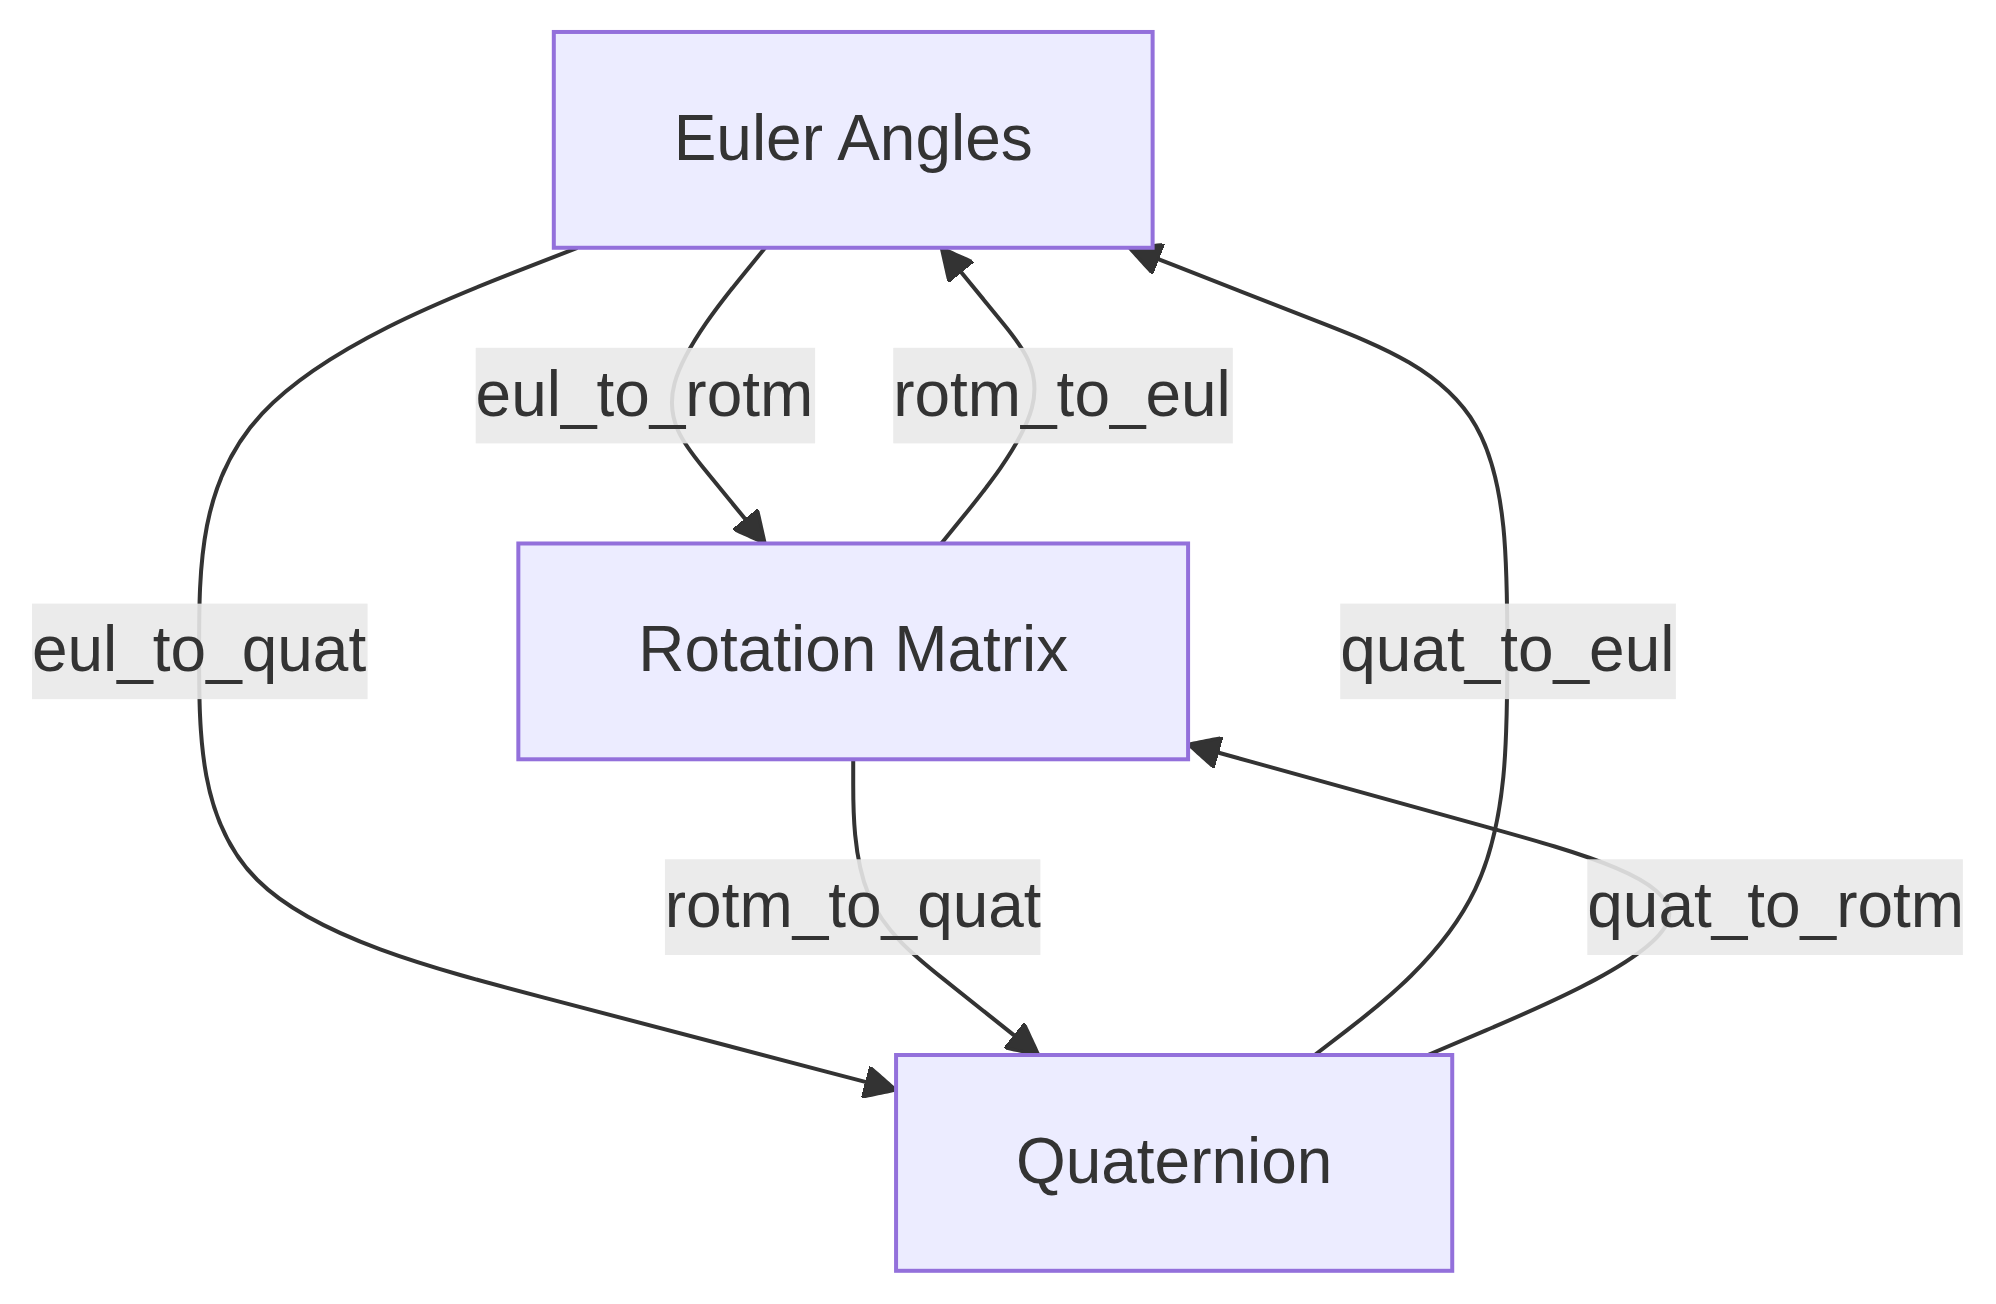
\includegraphics[width=5.2in,height=3.4in]{rawFiles/Kinematics/Kinematics_files/figure-latex/mermaid-figure-1.png}

\begin{longtable}[]{@{}
  >{\raggedright\arraybackslash}p{(\linewidth - 2\tabcolsep) * \real{0.4348}}
  >{\raggedright\arraybackslash}p{(\linewidth - 2\tabcolsep) * \real{0.5652}}@{}}
\toprule\noalign{}
\begin{minipage}[b]{\linewidth}\raggedright
Function
\end{minipage} & \begin{minipage}[b]{\linewidth}\raggedright
Description
\end{minipage} \\
\midrule\noalign{}
\endhead
\bottomrule\noalign{}
\endlastfoot
\texttt{eul\_to\_rotm(eul,\ order=\textquotesingle{}ZYX\textquotesingle{},\ deg=False)}
& Converts Euler angles (roll \(\phi\), pitch \(\theta\), yaw \(\psi\))
to a 3x3 rotation matrix that transforms vectors from the Body frame
\{b\} to the NED frame \{n\}. Assumes ZYX rotation order. Angles can be
in radians or degrees. \\
\texttt{rotm\_to\_eul(rotm,\ order=\textquotesingle{}ZYX\textquotesingle{},\ prev\_eul=None,\ deg=False,\ silent=True)}
& Converts a 3x3 rotation matrix back to Euler angles (roll \(\phi\),
pitch \(\theta\), yaw \(\psi\)). Handles potential ambiguities and
gimbal lock using previous Euler angles (\texttt{prev\_eul}) if
provided. Can output in radians or degrees. \\
\texttt{eul\_to\_quat(eul,\ order=\textquotesingle{}ZYX\textquotesingle{},\ deg=False)}
& Converts Euler angles (roll \(\phi\), pitch \(\theta\), yaw \(\psi\))
to a unit quaternion \([q_w, q_x, q_y, q_z]\). Assumes ZYX rotation
order. Angles can be in radians or degrees. \\
\texttt{quat\_to\_eul(quat,\ order=\textquotesingle{}ZYX\textquotesingle{},\ deg=False,\ prev\_quat=None,\ silent=True)}
& Converts a unit quaternion \([q_w, q_x, q_y, q_z]\) to Euler angles
(roll \(\phi\), pitch \(\theta\), yaw \(\psi\)). Handles potential
ambiguities using \texttt{prev\_quat} if provided. Can output in radians
or degrees. \\
\texttt{quat\_to\_rotm(quat)} & Converts a unit quaternion
\([q_w, q_x, q_y, q_z]\) to a 3x3 rotation matrix that transforms
vectors from the Body frame \{b\} to the NED frame \{n\}. \\
\texttt{rotm\_to\_quat(rotm)} & Converts a 3x3 rotation matrix (Body to
NED) to a unit quaternion \([q_w, q_x, q_y, q_z]\). \\
\end{longtable}

\subsection*{Quaternion Operations}\label{quaternion-operations}
\addcontentsline{toc}{subsection}{Quaternion Operations}

\begin{longtable}[]{@{}
  >{\raggedright\arraybackslash}p{(\linewidth - 2\tabcolsep) * \real{0.4348}}
  >{\raggedright\arraybackslash}p{(\linewidth - 2\tabcolsep) * \real{0.5652}}@{}}
\toprule\noalign{}
\begin{minipage}[b]{\linewidth}\raggedright
Function
\end{minipage} & \begin{minipage}[b]{\linewidth}\raggedright
Description
\end{minipage} \\
\midrule\noalign{}
\endhead
\bottomrule\noalign{}
\endlastfoot
\texttt{quat\_multiply(q1,\ q2)} & Multiplies two quaternions
\(\mathbf{q}_1 \otimes \mathbf{q}_2\). Order matters: represents
rotation \(\mathbf{q}_2\) followed by rotation \(\mathbf{q}_1\). \\
\texttt{quat\_conjugate(quat)} & Computes the conjugate of a quaternion
\(\mathbf{q}^* = [q_w, -q_x, -q_y, -q_z]^T\). \\
\texttt{rotate\_vec\_by\_quat(vec\_a,\ q\_a\_b)} & Rotates a 3D vector
\texttt{vec\_a} using the quaternion rotation \texttt{q\_a\_b}
(representing rotation from frame A to frame B) to get the vector in
frame B. Computes
\(\mathbf{v}_b' = \mathbf{q}_{a \to b} \otimes \mathbf{v}_a' \otimes \mathbf{q}_{a \to b}^*\). \\
\end{longtable}

\subsection*{Rate Calculations}\label{rate-calculations}
\addcontentsline{toc}{subsection}{Rate Calculations}

\begin{longtable}[]{@{}
  >{\raggedright\arraybackslash}p{(\linewidth - 2\tabcolsep) * \real{0.4348}}
  >{\raggedright\arraybackslash}p{(\linewidth - 2\tabcolsep) * \real{0.5652}}@{}}
\toprule\noalign{}
\begin{minipage}[b]{\linewidth}\raggedright
Function
\end{minipage} & \begin{minipage}[b]{\linewidth}\raggedright
Description
\end{minipage} \\
\midrule\noalign{}
\endhead
\bottomrule\noalign{}
\endlastfoot
\texttt{eul\_rate\_matrix(eul,\ order=\textquotesingle{}ZYX\textquotesingle{},\ deg=False)}
& Computes the 3x3 transformation matrix
\(\mathbf{T}(\boldsymbol{\eta})\) that relates body-frame angular
velocity \(\boldsymbol{\omega}^b\) to Euler angle rates
\(\dot{\boldsymbol{\eta}}\) via
\(\dot{\boldsymbol{\eta}} = \mathbf{T}(\boldsymbol{\eta}) \boldsymbol{\omega}^b\).
Assumes ZYX order. \\
\texttt{quat\_rate\_matrix(quat)} & Computes the 4x3 transformation
matrix \(\mathbf{E}(\mathbf{q})\) that relates body-frame angular
velocity \(\boldsymbol{\omega}^b\) to quaternion rates
\(\dot{\mathbf{q}}\) via
\(\dot{\mathbf{q}} = \frac{1}{2} \mathbf{E}(\mathbf{q}) \boldsymbol{\omega}^b\). \\
\texttt{eul\_rate(eul,\ w,\ order=\textquotesingle{}ZYX\textquotesingle{})}
& Calculates Euler angle rates
\([\dot{\phi}, \dot{\theta}, \dot{\psi}]\) given current Euler angles
\texttt{eul} and body-frame angular velocity \texttt{w} =
\([p, q, r]^T\). Uses \texttt{eul\_rate\_matrix}. \\
\texttt{quat\_rate(quat,\ w)} & Calculates quaternion rates
\([\dot{q}_w, \dot{q}_x, \dot{q}_y, \dot{q}_z]\) given the current
quaternion \texttt{quat} and body-frame angular velocity \texttt{w} =
\([p, q, r]^T\). Uses \texttt{quat\_rate\_matrix}. \\
\texttt{deul\_dquat(quat)} & Computes the 3x4 Jacobian matrix
\(\frac{\partial \boldsymbol{\eta}}{\partial \mathbf{q}}\), representing
the partial derivatives of Euler angles with respect to quaternion
components. \\
\texttt{dquat\_deul(quat)} & Computes the 4x3 Jacobian matrix
\(\frac{\partial \mathbf{q}}{\partial \boldsymbol{\eta}}\), representing
the partial derivatives of quaternion components with respect to Euler
angles. Requires converting \texttt{quat} to \texttt{eul} internally
first. \\
\end{longtable}

\subsection*{Navigation Functions}\label{navigation-functions}
\addcontentsline{toc}{subsection}{Navigation Functions}

\begin{longtable}[]{@{}
  >{\raggedright\arraybackslash}p{(\linewidth - 2\tabcolsep) * \real{0.4348}}
  >{\raggedright\arraybackslash}p{(\linewidth - 2\tabcolsep) * \real{0.5652}}@{}}
\toprule\noalign{}
\begin{minipage}[b]{\linewidth}\raggedright
Function
\end{minipage} & \begin{minipage}[b]{\linewidth}\raggedright
Description
\end{minipage} \\
\midrule\noalign{}
\endhead
\bottomrule\noalign{}
\endlastfoot
\texttt{ssa(ang,\ deg=False)} & Converts an angle (in radians or
degrees) to its smallest signed angle representation within the range
\((-\pi, \pi]\) radians or \((-180, 180]\) degrees. \\
\texttt{clip(value,\ threshold)} & Limits the input \texttt{value} to
the range \texttt{{[}-threshold,\ threshold{]}}. \\
\texttt{ned\_to\_llh(ned,\ llh0)} & Converts a position vector
\texttt{ned} = {[}North, East, Down{]} relative to a reference point
\texttt{llh0} = {[}lat0, lon0, h0{]} into absolute geodetic coordinates
\texttt{llh} = {[}latitude, longitude, height{]}. Uses WGS84 ellipsoid
model. \\
\texttt{llh\_to\_ned(llh,\ llh0)} & Converts an absolute geodetic
position \texttt{llh} = {[}lat, lon, h{]} into a local NED position
vector \texttt{ned} = {[}North, East, Down{]} relative to a reference
point \texttt{llh0} = {[}lat0, lon0, h0{]}. Uses WGS84 ellipsoid
model. \\
\texttt{generate\_waypoints()} & Generates a predefined sequence of
waypoints as LLH coordinates for a rectangular survey pattern relative
to a specific datum location (IITM lake). Returns a numpy array of
{[}lat, lon, height{]} waypoints. \\
\texttt{rotm\_ned\_to\_ecef(llh)} & Computes the 3x3 rotation matrix
\(\mathbf{R}_n^e\) that transforms vectors from the local NED frame
(defined at \texttt{llh}) to the ECEF frame. \\
\end{longtable}

\subsection*{Utility Functions}\label{utility-functions}
\addcontentsline{toc}{subsection}{Utility Functions}

\begin{longtable}[]{@{}
  >{\raggedright\arraybackslash}p{(\linewidth - 2\tabcolsep) * \real{0.4348}}
  >{\raggedright\arraybackslash}p{(\linewidth - 2\tabcolsep) * \real{0.5652}}@{}}
\toprule\noalign{}
\begin{minipage}[b]{\linewidth}\raggedright
Function
\end{minipage} & \begin{minipage}[b]{\linewidth}\raggedright
Description
\end{minipage} \\
\midrule\noalign{}
\endhead
\bottomrule\noalign{}
\endlastfoot
\texttt{Smat(vec)} & Creates the 3x3 skew-symmetric matrix
\(\mathbf{S}(\mathbf{v})\) corresponding to the input 3D vector
\texttt{vec}. Used for representing cross products as matrix
multiplications
(\(\mathbf{a} \times \mathbf{b} = \mathbf{S}(\mathbf{a}) \mathbf{b}\)). \\
\end{longtable}

\section*{Usage Examples}\label{usage-examples}
\addcontentsline{toc}{section}{Usage Examples}

\markright{Usage Examples}

\subsection*{Coordinate
Transformations}\label{coordinate-transformations}
\addcontentsline{toc}{subsection}{Coordinate Transformations}

\begin{Shaded}
\begin{Highlighting}[]
\ImportTok{import}\NormalTok{ numpy }\ImportTok{as}\NormalTok{ np}
\ImportTok{from}\NormalTok{ mav\_simulator.module\_kinematics }\ImportTok{import}\NormalTok{ eul\_to\_rotm, llh\_to\_ned}

\CommentTok{\# Convert Euler angles to rotation matrix}
\NormalTok{euler\_angles }\OperatorTok{=}\NormalTok{ np.array([}\FloatTok{0.1}\NormalTok{, }\FloatTok{0.2}\NormalTok{, }\FloatTok{0.3}\NormalTok{])  }\CommentTok{\# [roll, pitch, yaw] in radians}
\NormalTok{R }\OperatorTok{=}\NormalTok{ eul\_to\_rotm(euler\_angles)  }\CommentTok{\# Rotation matrix}

\CommentTok{\# Convert latitude, longitude, height to NED coordinates}
\NormalTok{reference\_point }\OperatorTok{=}\NormalTok{ np.array([}\FloatTok{60.0}\NormalTok{, }\FloatTok{10.0}\NormalTok{, }\FloatTok{0.0}\NormalTok{])  }\CommentTok{\# [lat, lon, height]}
\NormalTok{target\_point }\OperatorTok{=}\NormalTok{ np.array([}\FloatTok{60.001}\NormalTok{, }\FloatTok{10.001}\NormalTok{, }\FloatTok{10.0}\NormalTok{])  }\CommentTok{\# [lat, lon, height]}
\NormalTok{ned\_coords }\OperatorTok{=}\NormalTok{ llh\_to\_ned(target\_point, reference\_point)}
\end{Highlighting}
\end{Shaded}

\subsection*{Rotation Representations}\label{rotation-representations}
\addcontentsline{toc}{subsection}{Rotation Representations}

\begin{Shaded}
\begin{Highlighting}[]
\ImportTok{from}\NormalTok{ mav\_simulator.module\_kinematics }\ImportTok{import}\NormalTok{ eul\_to\_quat, quat\_to\_rotm}

\CommentTok{\# Convert from Euler angles to quaternion}
\NormalTok{euler\_angles }\OperatorTok{=}\NormalTok{ np.array([}\FloatTok{0.1}\NormalTok{, }\FloatTok{0.2}\NormalTok{, }\FloatTok{0.3}\NormalTok{])  }\CommentTok{\# [roll, pitch, yaw] in radians}
\NormalTok{quaternion }\OperatorTok{=}\NormalTok{ eul\_to\_quat(euler\_angles)}

\CommentTok{\# Convert from quaternion to rotation matrix}
\NormalTok{R }\OperatorTok{=}\NormalTok{ quat\_to\_rotm(quaternion)}
\end{Highlighting}
\end{Shaded}

\section*{Best Practices}\label{best-practices}
\addcontentsline{toc}{section}{Best Practices}

\markright{Best Practices}

\begin{itemize}
\tightlist
\item
  Use the \texttt{ssa()} function to normalize angles when working with
  Euler angles
\item
  Be consistent with the rotation order convention throughout your code
  (the default is `ZYX')
\item
  When transforming between frames, always keep track of the reference
  frames involved
\end{itemize}

\bookmarksetup{startatroot}

\chapter*{Dynamics}\label{dynamics}
\addcontentsline{toc}{chapter}{Dynamics}

\markboth{Dynamics}{Dynamics}

\section*{Overview}\label{overview-2}
\addcontentsline{toc}{section}{Overview}

\markright{Overview}

The Dynamics modules (\texttt{class\_vessel.py} and
\texttt{calculate\_hydrodynamics.py}) implement the mathematical
foundation for simulating the motion of marine vehicles through water.
The simulator uses Fossen's nonlinear 6-DOF equation of motion:

\[M\dot{\nu}+C(\nu)\nu+D(\nu)\nu+g(\eta) = \tau\]

where,

\begin{itemize}
\tightlist
\item
  \(M = M_{RB} + M_A\) is the mass matrix, combining rigid body mass
  \(M_{RB}\) and added mass \(M_A\)
\item
  \(C(\nu) = C_{RB}(\nu) + C_A(\nu)\) is the Coriolis and centripetal
  matrix
\item
  \(D(\nu)\) is the hydrodynamic damping matrix
\item
  \(g(\eta)\) is the gravitational and buoyancy force vector
\item
  \(\tau\) is the control force vector from thrusters and control
  surfaces
\item
  \(\nu = [u, v, w, p, q, r]^T\) is the velocity vector in the body
  frame
\item
  \(\eta = [x, y, z, \phi, \theta, \psi]^T\) is the position and
  orientation vector
\end{itemize}

\begin{tcolorbox}[enhanced jigsaw, colback=white, toptitle=1mm, colframe=quarto-callout-tip-color-frame, rightrule=.15mm, breakable, title=\textcolor{quarto-callout-tip-color}{\faLightbulb}\hspace{0.5em}{Tip}, toprule=.15mm, opacitybacktitle=0.6, opacityback=0, coltitle=black, leftrule=.75mm, colbacktitle=quarto-callout-tip-color!10!white, arc=.35mm, titlerule=0mm, bottomtitle=1mm, bottomrule=.15mm, left=2mm]

The dynamics modules serve as the core of the simulation, determining
how forces and moments translate into vessel motion through water.

\end{tcolorbox}

\section*{State Representation}\label{state-representation}
\addcontentsline{toc}{section}{State Representation}

\markright{State Representation}

The vessel state is represented as a vector combining velocities,
position, orientation, control surface angles, and thruster states:

\(\text{state} = [\nu^T, \eta_{pos}^T, \eta_{rot}^T, \delta^T, n^T]^T\)

Where:

\begin{itemize}
\tightlist
\item
  \(\nu = [u, v, w, p, q, r]^T\) are the linear and angular velocities
  in the body frame
\item
  \(\eta_{pos} = [x, y, z]^T\) is the position in the NED frame
\item
  \(\eta_{rot}\) is the orientation, either as Euler angles
  \([\phi, \theta, \psi]^T\) or quaternion \([q_0, q_1, q_2, q_3]^T\)
\item
  \(\delta\) is the vector of control surface angles
\item
  \(n\) is the vector of thruster rotational speeds (RPM)
\end{itemize}

\section*{Components of the Dynamic
Equation}\label{components-of-the-dynamic-equation}
\addcontentsline{toc}{section}{Components of the Dynamic Equation}

\markright{Components of the Dynamic Equation}

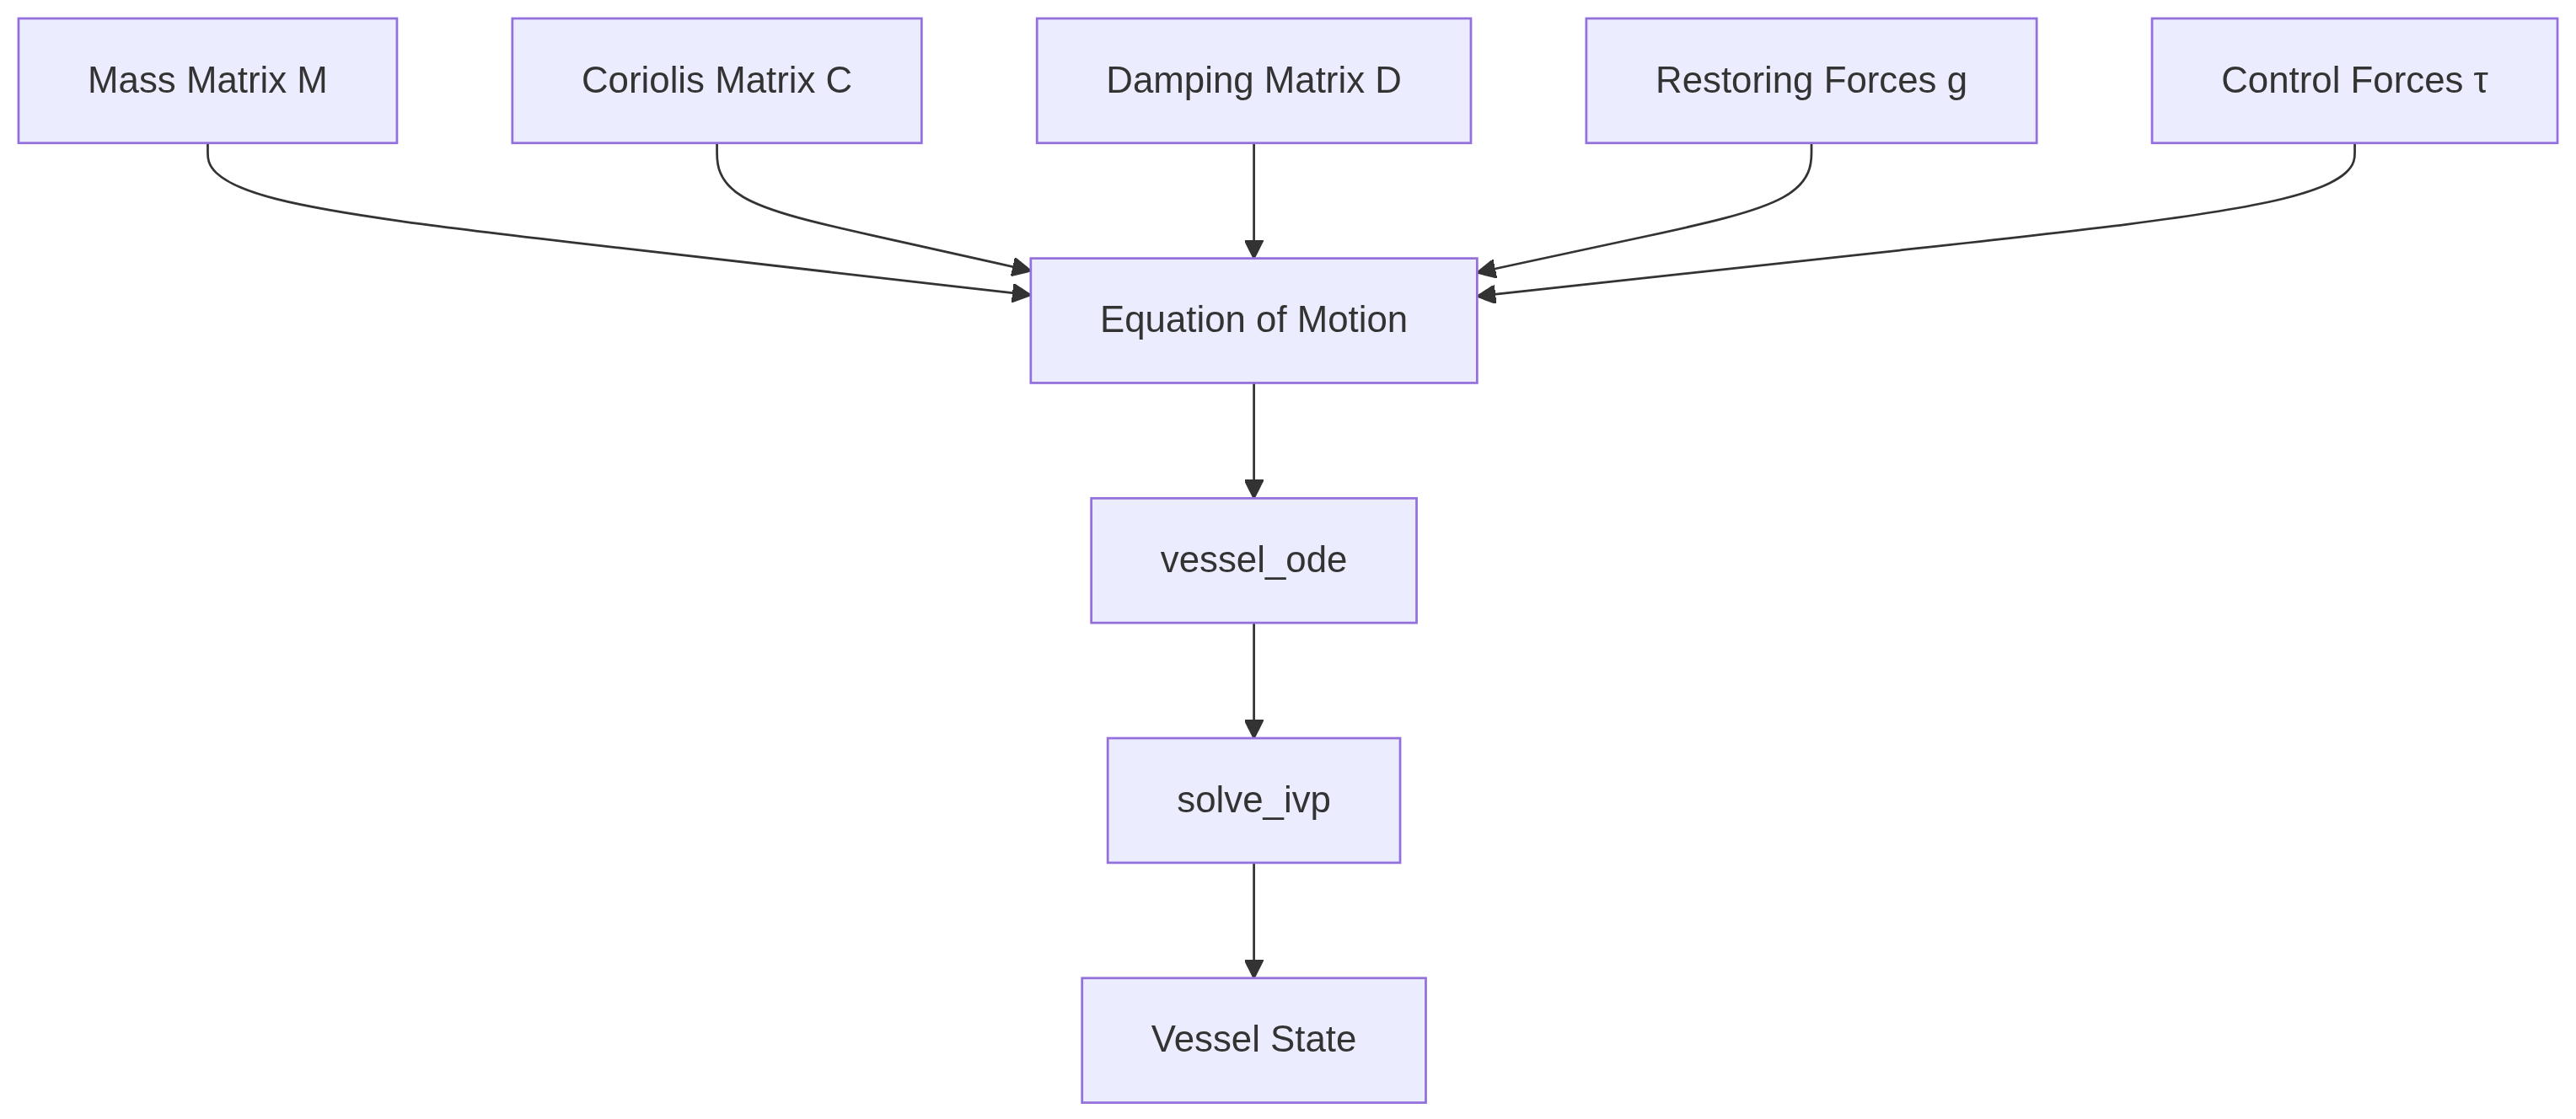
\includegraphics[width=11.63in,height=5.06in]{rawFiles/Dynamics/Dynamics_files/figure-latex/mermaid-figure-1.png}

\subsection*{\texorpdfstring{Mass Matrix
(\(M\))}{Mass Matrix (M)}}\label{mass-matrix-m}
\addcontentsline{toc}{subsection}{Mass Matrix (\(M\))}

The mass matrix \(M\) combines the rigid-body inertia matrix \(M_{RB}\)
and the added mass matrix \(M_A\):

\[M = M_{RB} + M_A\]

\subsubsection*{\texorpdfstring{Rigid-body Mass Matrix
(\(M_{RB}\))}{Rigid-body Mass Matrix (M\_\{RB\})}}\label{rigid-body-mass-matrix-m_rb}
\addcontentsline{toc}{subsubsection}{Rigid-body Mass Matrix
(\(M_{RB}\))}

The rigid-body mass matrix is generated in the
\texttt{\_generate\_mass\_matrix} method in
\texttt{calculate\_hydrodynamics.py}:

\[M_{RB} = \begin{bmatrix} m I_{3 \times 3} & -m S(r_G) \\ m S(r_G) & I_G \end{bmatrix}\]

Where:

\begin{itemize}
\tightlist
\item
  \(m\) is the vessel mass
\item
  \(I_{3 \times 3}\) is the 3×3 identity matrix
\item
  \(r_G\) is the center of gravity vector relative to the origin of the
  body frame
\item
  \(S(r_G)\) is the skew-symmetric matrix of \(r_G\) (implemented by
  \texttt{Smat()} in \texttt{module\_kinematics.py})
\item
  \(I_G\) is the inertia tensor calculated from the radii of gyration
\end{itemize}

\begin{Shaded}
\begin{Highlighting}[]
\KeywordTok{def}\NormalTok{ \_generate\_mass\_matrix(}\VariableTok{self}\NormalTok{, CG, mass, gyration):}
    \CommentTok{\# Calculate gyration tensor about vessel frame}
\NormalTok{    xprdct2 }\OperatorTok{=}\NormalTok{ np.diag(gyration)}\OperatorTok{**}\DecValTok{2} \OperatorTok{{-}}\NormalTok{ Smat(CG)}\OperatorTok{@}\NormalTok{Smat(CG)}
    
    \CommentTok{\# Generate the inertia matrix using radii of gyration}
\NormalTok{    inertia\_matrix }\OperatorTok{=}\NormalTok{ xprdct2 }\OperatorTok{*}\NormalTok{ mass}

    \CommentTok{\# Generate the mass matrix}
\NormalTok{    mass\_matrix }\OperatorTok{=}\NormalTok{ np.zeros((}\DecValTok{6}\NormalTok{,}\DecValTok{6}\NormalTok{))}
\NormalTok{    mass\_matrix[}\DecValTok{0}\NormalTok{:}\DecValTok{3}\NormalTok{][:, }\DecValTok{0}\NormalTok{:}\DecValTok{3}\NormalTok{] }\OperatorTok{=}\NormalTok{ mass }\OperatorTok{*}\NormalTok{ np.eye(}\DecValTok{3}\NormalTok{)}
\NormalTok{    mass\_matrix[}\DecValTok{3}\NormalTok{:}\DecValTok{6}\NormalTok{][:, }\DecValTok{3}\NormalTok{:}\DecValTok{6}\NormalTok{] }\OperatorTok{=}\NormalTok{ inertia\_matrix}
\NormalTok{    mass\_matrix[}\DecValTok{0}\NormalTok{:}\DecValTok{3}\NormalTok{][:, }\DecValTok{3}\NormalTok{:}\DecValTok{6}\NormalTok{] }\OperatorTok{=} \OperatorTok{{-}}\NormalTok{Smat(CG) }\OperatorTok{*}\NormalTok{ mass}
\NormalTok{    mass\_matrix[}\DecValTok{3}\NormalTok{:}\DecValTok{6}\NormalTok{][:, }\DecValTok{0}\NormalTok{:}\DecValTok{3}\NormalTok{] }\OperatorTok{=}\NormalTok{ Smat(CG) }\OperatorTok{*}\NormalTok{ mass}

    \ControlFlowTok{return}\NormalTok{ mass\_matrix}
\end{Highlighting}
\end{Shaded}

\subsubsection*{\texorpdfstring{Added Mass Matrix
(\(M_A\))}{Added Mass Matrix (M\_A)}}\label{added-mass-matrix-m_a}
\addcontentsline{toc}{subsubsection}{Added Mass Matrix (\(M_A\))}

The added mass matrix represents the added inertia due to accelerating
the surrounding fluid. It's calculated from hydrodynamic data obtained
from \href{https://hydra.hydratech.in/}{HydRA} (You can also enter
custom hydrodynamics added mass coefficients (example Y\_vd) in the
\texttt{hydrodynamics.yml} input file instead of using HydRA, as
discussed in the \href{../Inputs/inputs.qmd}{Inputs} section).

\[M_A = \begin{bmatrix} A_{11} & A_{12} \\ A_{21} & A_{22} \end{bmatrix}\]

\begin{longtable}[]{@{}
  >{\raggedright\arraybackslash}p{(\linewidth - 2\tabcolsep) * \real{0.4348}}
  >{\raggedright\arraybackslash}p{(\linewidth - 2\tabcolsep) * \real{0.5652}}@{}}
\toprule\noalign{}
\begin{minipage}[b]{\linewidth}\raggedright
Function
\end{minipage} & \begin{minipage}[b]{\linewidth}\raggedright
Description
\end{minipage} \\
\midrule\noalign{}
\endhead
\bottomrule\noalign{}
\endlastfoot
\texttt{calculate\_added\_mass\_from\_hydra(hydra\_file)} & Computes the
added mass matrix from HydRA data file containing frequency-dependent
hydrodynamic coefficients. Extracts zero-frequency added mass for most
terms, but computes heave, roll, and pitch terms at their natural
frequencies for better accuracy. \\
\end{longtable}

\begin{Shaded}
\begin{Highlighting}[]
\KeywordTok{def}\NormalTok{ calculate\_added\_mass\_from\_hydra(}\VariableTok{self}\NormalTok{, hydra\_file):}
    \CommentTok{\# Load hydrodynamic data}
    \ControlFlowTok{with} \BuiltInTok{open}\NormalTok{(hydra\_file, }\StringTok{\textquotesingle{}r\textquotesingle{}}\NormalTok{) }\ImportTok{as} \BuiltInTok{file}\NormalTok{:}
\NormalTok{        mdict }\OperatorTok{=}\NormalTok{ json.load(}\BuiltInTok{file}\NormalTok{)}
    
    \CommentTok{\# Extract arrays from data}
\NormalTok{    omg }\OperatorTok{=}\NormalTok{ np.array(mdict[}\StringTok{\textquotesingle{}w\textquotesingle{}}\NormalTok{])      }\CommentTok{\# Frequency array}
\NormalTok{    AM }\OperatorTok{=}\NormalTok{ np.array(mdict[}\StringTok{\textquotesingle{}AM\textquotesingle{}}\NormalTok{])      }\CommentTok{\# Added mass array}
    
    \CommentTok{\# Extract zero{-}frequency added mass}
\NormalTok{    A\_zero }\OperatorTok{=}\NormalTok{ AM[}\DecValTok{1}\NormalTok{, :, :, }\DecValTok{0}\NormalTok{, }\DecValTok{0}\NormalTok{]}
    
    \CommentTok{\# Calculate natural frequencies and}
    \CommentTok{\# interpolate added mass at those frequencies}
    \CommentTok{\# ...}
    
    \CommentTok{\# Return properly transformed added mass matrix}
    \ControlFlowTok{return}\NormalTok{ A}
\end{Highlighting}
\end{Shaded}

\begin{tcolorbox}[enhanced jigsaw, colback=white, toptitle=1mm, colframe=quarto-callout-note-color-frame, rightrule=.15mm, breakable, title=\textcolor{quarto-callout-note-color}{\faInfo}\hspace{0.5em}{Note}, toprule=.15mm, opacitybacktitle=0.6, opacityback=0, coltitle=black, leftrule=.75mm, colbacktitle=quarto-callout-note-color!10!white, arc=.35mm, titlerule=0mm, bottomtitle=1mm, bottomrule=.15mm, left=2mm]

The added mass calculated from HydRA is in ENU frame and so it is
converted to NED frame in the
\texttt{calculate\_added\_mass\_from\_hydra} function.

\end{tcolorbox}

\subsection*{Coriolis and Centripetal
Matrix}\label{coriolis-and-centripetal-matrix}
\addcontentsline{toc}{subsection}{Coriolis and Centripetal Matrix}

The Coriolis matrix (\(C(\nu)\)) accounts for forces arising from motion
in a rotating reference frame (Body frame is rotating with respect to
NED frame):

\[C(\nu) = C_{RB}(\nu) + C_A(\nu)\]

These matrices are calculated using:

\[C_{RB}(\nu) = \begin{bmatrix} 0_{3 \times 3} & -S(M_{11} v_1 + M_{12} v_2) \\ 
-S(M_{11} v_1 + M_{12} v_2) & -S(M_{21} v_1 + M_{22} v_2) \end{bmatrix}\]

\[C_A(\nu) = \begin{bmatrix} 0_{3 \times 3} & -S(A_{11} v_1 + A_{12} v_2) \\ 
-S(A_{11} v_1 + A_{12} v_2) & -S(A_{21} v_1 + A_{22} v_2) \end{bmatrix}\]

Where \(v_1 = [u, v, w]^T\) and \(v_2 = [p, q, r]^T\) are the linear and
angular velocity components of \(\nu\).

\begin{longtable}[]{@{}
  >{\raggedright\arraybackslash}p{(\linewidth - 2\tabcolsep) * \real{0.4348}}
  >{\raggedright\arraybackslash}p{(\linewidth - 2\tabcolsep) * \real{0.5652}}@{}}
\toprule\noalign{}
\begin{minipage}[b]{\linewidth}\raggedright
Function
\end{minipage} & \begin{minipage}[b]{\linewidth}\raggedright
Description
\end{minipage} \\
\midrule\noalign{}
\endhead
\bottomrule\noalign{}
\endlastfoot
\texttt{calculate\_coriolis\_matrices(vel)} & Computes the rigid body
and added mass Coriolis-centripetal matrices based on the current
velocity state. Returns a tuple of \((C_{RB}, C_A)\) matrices. \\
\end{longtable}

\subsection*{Damping Matrix}\label{damping-matrix}
\addcontentsline{toc}{subsection}{Damping Matrix}

The damping matrix (\(D(\nu)\)) represents hydrodynamic resistance
forces and is typically modeled as:

\[D(\nu) = D_{linear} + D_{nonlinear}(\nu)\]

In the implementation, damping is handled through hydrodynamic
coefficients (entered in the \texttt{hydrodynamics.yml} input file)
rather than an explicit matrix:

\begin{longtable}[]{@{}
  >{\raggedright\arraybackslash}p{(\linewidth - 2\tabcolsep) * \real{0.4348}}
  >{\raggedright\arraybackslash}p{(\linewidth - 2\tabcolsep) * \real{0.5652}}@{}}
\toprule\noalign{}
\begin{minipage}[b]{\linewidth}\raggedright
Function
\end{minipage} & \begin{minipage}[b]{\linewidth}\raggedright
Description
\end{minipage} \\
\midrule\noalign{}
\endhead
\bottomrule\noalign{}
\endlastfoot
\texttt{hydrodynamic\_forces(vel)} & Computes hydrodynamic damping
forces by applying coefficients to velocity components. Supports linear,
quadratic, and cross-terms. \\
\texttt{cross\_flow\_drag()} & Estimates sway-yaw damping coefficients
for surface vessels using strip theory and Hoerner's cross-flow drag. \\
\texttt{cross\_flow\_drag\_AUV()} & Similar to
\texttt{cross\_flow\_drag()} but includes heave-pitch calculations for
AUVs. \\
\texttt{hoerner()} & Implements Hoerner's method for computing 2D drag
coefficients based on section beam-to-draft ratio. \\
\end{longtable}

The coefficients follow a naming convention that indicates which
force/moment they affect and which velocity components are involved (you
can enter any custom hydrodynamic coefficients in the
\texttt{hydrodynamics.yml} input file and it will be handled by the
function for force calculations):

\begin{itemize}
\tightlist
\item
  Linear damping: \texttt{X\_u}, \texttt{Y\_v}, \texttt{Z\_w},
  \texttt{K\_p}, \texttt{M\_q}, \texttt{N\_r}
\item
  Quadratic damping: \texttt{X\_u\_au}, \texttt{Y\_v\_av},
  \texttt{Z\_w\_aw}, etc. (the \texttt{a} indicates absolute value)
\item
  Cross-coupling: \texttt{X\_vr}, \texttt{Y\_ur}, \texttt{N\_uv}, etc.
\end{itemize}

\begin{Shaded}
\begin{Highlighting}[]
\KeywordTok{def}\NormalTok{ hydrodynamic\_forces(}\VariableTok{self}\NormalTok{, vel):}
    \CommentTok{\# Extract velocities}
\NormalTok{    u, v, w, p, q, r }\OperatorTok{=}\NormalTok{ vel}
    
    \CommentTok{\# Initialize forces vector}
\NormalTok{    F }\OperatorTok{=}\NormalTok{ np.zeros(}\DecValTok{6}\NormalTok{)}
    
    \CommentTok{\# Map velocity components to values}
\NormalTok{    vel\_map }\OperatorTok{=}\NormalTok{ \{}\StringTok{\textquotesingle{}u\textquotesingle{}}\NormalTok{: u, }\StringTok{\textquotesingle{}v\textquotesingle{}}\NormalTok{: v, }\StringTok{\textquotesingle{}w\textquotesingle{}}\NormalTok{: w, }\StringTok{\textquotesingle{}p\textquotesingle{}}\NormalTok{: p, }\StringTok{\textquotesingle{}q\textquotesingle{}}\NormalTok{: q, }\StringTok{\textquotesingle{}r\textquotesingle{}}\NormalTok{: r\}}
    
    \CommentTok{\# Process each hydrodynamic coefficient}
    \ControlFlowTok{for}\NormalTok{ coeff\_name, coeff\_value }\KeywordTok{in} \VariableTok{self}\NormalTok{.hydrodynamics.items():}
        \ControlFlowTok{if}\NormalTok{ coeff\_value }\OperatorTok{==} \DecValTok{0}\NormalTok{: }\ControlFlowTok{continue}
        
\NormalTok{        parts }\OperatorTok{=}\NormalTok{ coeff\_name.split(}\StringTok{\textquotesingle{}\_\textquotesingle{}}\NormalTok{)}
\NormalTok{        force\_dir }\OperatorTok{=}\NormalTok{ parts[}\DecValTok{0}\NormalTok{]}
        \ControlFlowTok{if}\NormalTok{ force\_dir }\KeywordTok{not} \KeywordTok{in} \VariableTok{self}\NormalTok{.force\_indices: }\ControlFlowTok{continue}
        
        \CommentTok{\# Calculate force contribution}
\NormalTok{        force }\OperatorTok{=}\NormalTok{ coeff\_value}
        \ControlFlowTok{for}\NormalTok{ component }\KeywordTok{in}\NormalTok{ parts[}\DecValTok{1}\NormalTok{:]:}
            \ControlFlowTok{if}\NormalTok{ component.startswith(}\StringTok{\textquotesingle{}a\textquotesingle{}}\NormalTok{) }\KeywordTok{and} \BuiltInTok{len}\NormalTok{(component) }\OperatorTok{\textgreater{}} \DecValTok{1}\NormalTok{:}
                \CommentTok{\# Absolute value term (e.g., u|u|)}
\NormalTok{                v\_char }\OperatorTok{=}\NormalTok{ component[}\DecValTok{1}\NormalTok{:]}
\NormalTok{                force }\OperatorTok{*=} \BuiltInTok{abs}\NormalTok{(vel\_map[v\_char])}
            \ControlFlowTok{elif}\NormalTok{ component }\KeywordTok{in}\NormalTok{ vel\_map:}
                \CommentTok{\# Regular term}
\NormalTok{                force }\OperatorTok{*=}\NormalTok{ vel\_map[component]}
                
        \CommentTok{\# Add to force vector}
\NormalTok{        F[}\VariableTok{self}\NormalTok{.force\_indices[force\_dir]] }\OperatorTok{+=}\NormalTok{ force}
        
    \ControlFlowTok{return}\NormalTok{ F}
\end{Highlighting}
\end{Shaded}

\subsection*{Restoring Forces}\label{restoring-forces}
\addcontentsline{toc}{subsection}{Restoring Forces}

The restoring forces (\(g(\eta)\)) include gravitational and buoyancy
effects:

\[g(\eta) = \begin{bmatrix} 
(W - B) \sin \theta \\ 
-(W - B) \cos \theta \sin \phi \\ 
-(W - B) \cos \theta \cos \phi \\ 
-(y_G W - y_B B) \cos \theta \cos \phi + (z_G W - z_B B) \cos \theta \sin \phi \\ 
(z_G W - z_B B) \sin \theta + (x_G W - x_B B) \cos \theta \cos \phi \\ 
-(x_G W - x_B B) \cos \theta \sin \phi - (y_G W - y_B B) \sin \theta 
\end{bmatrix}\]

Where:

\begin{itemize}
\tightlist
\item
  \(W = mg\) is the weight
\item
  \(B = \rho g \nabla\) is the buoyancy force (with \(\nabla\) being the
  displaced volume)
\item
  \(r_G = [x_G, y_G, z_G]^T\) is the center of gravity mentioned in the
  \texttt{geometry.yml} input file
\item
  \(r_B = [x_B, y_B, z_B]^T\) is the center of buoyancy mentioned in the
  \texttt{geometry.yml} input file
\end{itemize}

\begin{longtable}[]{@{}
  >{\raggedright\arraybackslash}p{(\linewidth - 2\tabcolsep) * \real{0.4348}}
  >{\raggedright\arraybackslash}p{(\linewidth - 2\tabcolsep) * \real{0.5652}}@{}}
\toprule\noalign{}
\begin{minipage}[b]{\linewidth}\raggedright
Function
\end{minipage} & \begin{minipage}[b]{\linewidth}\raggedright
Description
\end{minipage} \\
\midrule\noalign{}
\endhead
\bottomrule\noalign{}
\endlastfoot
\texttt{gravitational\_forces(phi,\ theta)} & Computes the gravitational
and buoyancy forces and moments as a function of roll and pitch
angles. \\
\end{longtable}

\subsection*{Control Forces}\label{control-forces}
\addcontentsline{toc}{subsection}{Control Forces}

The control forces vector \(\tau\) represents the combined effect of
control surfaces and thrusters.\#\#\#\# Control Surface Forces

\begin{longtable}[]{@{}
  >{\raggedright\arraybackslash}p{(\linewidth - 2\tabcolsep) * \real{0.4348}}
  >{\raggedright\arraybackslash}p{(\linewidth - 2\tabcolsep) * \real{0.5652}}@{}}
\toprule\noalign{}
\begin{minipage}[b]{\linewidth}\raggedright
Function
\end{minipage} & \begin{minipage}[b]{\linewidth}\raggedright
Description
\end{minipage} \\
\midrule\noalign{}
\endhead
\bottomrule\noalign{}
\endlastfoot
\texttt{control\_forces(delta)} & Calculates forces and moments
generated by control surfaces (rudders, fins, etc.) based on their
deflection angles \(\delta\). Supports both hydrodynamic
coefficient-based and aerofoil-based calculation methods. \\
\end{longtable}

For hydrodynamic coefficient-based calculation: - Forces are calculated
as \(\tau_i = C_{i\delta} \delta\), where \(C_{i\delta}\) is the control
coefficient mentioned in the \texttt{control\_surface\_hydrodynamics} in
the \texttt{control\_surfaces.yml} input file

For aerofoil-based calculation:

\begin{itemize}
\tightlist
\item
  Local velocity at the control surface is calculated considering vessel
  motion (automatically done)
\item
  Angle of attack is determined from flow direction and surface
  deflection
\item
  Lift and drag forces are calculated using NACA airfoil data (path to
  the NACA file is mentioned in the \texttt{control\_surfaces.yml} input
  file)
\item
  Forces are transformed to the body frame and a generalized force
  vector is returned
\end{itemize}

\subsubsection*{Thruster Forces}\label{thruster-forces}
\addcontentsline{toc}{subsubsection}{Thruster Forces}

\begin{longtable}[]{@{}
  >{\raggedright\arraybackslash}p{(\linewidth - 2\tabcolsep) * \real{0.4348}}
  >{\raggedright\arraybackslash}p{(\linewidth - 2\tabcolsep) * \real{0.5652}}@{}}
\toprule\noalign{}
\begin{minipage}[b]{\linewidth}\raggedright
Function
\end{minipage} & \begin{minipage}[b]{\linewidth}\raggedright
Description
\end{minipage} \\
\midrule\noalign{}
\endhead
\bottomrule\noalign{}
\endlastfoot
\texttt{thruster\_forces(n\_prop)} & Calculates forces and moments from
propellers/thrusters based on their rotational speeds \(n\) in RPM.
Models thrust using propeller theory with advance ratio and thrust
coefficients. \\
\end{longtable}

The thrust calculation follows the form:
\[X_{prop} = K_T \rho D^4 |n| n\]

Where:

\begin{itemize}
\tightlist
\item
  \(K_T\) is the thrust coefficient (approximated as \(K_{T,J=0}(1-J)\)
  with \(J\) being the advance ratio)
\item
  \(\rho\) is the water density
\item
  \(D\) is the propeller diameter
\item
  \(n\) is the propeller speed in revolutions per second
\end{itemize}

\section*{Vessel ODE and Simulation}\label{vessel-ode-and-simulation}
\addcontentsline{toc}{section}{Vessel ODE and Simulation}

\markright{Vessel ODE and Simulation}

The vessel dynamics are implemented as an ordinary differential equation
(ODE) in the \texttt{vessel\_ode(t,\ state)} method, which computes the
state derivatives:

\begin{Shaded}
\begin{Highlighting}[]
\KeywordTok{def}\NormalTok{ vessel\_ode(}\VariableTok{self}\NormalTok{, t, state):}
    \CommentTok{\# Extract state components}
\NormalTok{    vel }\OperatorTok{=}\NormalTok{ state[}\DecValTok{0}\NormalTok{:}\DecValTok{6}\NormalTok{]  }\CommentTok{\# [u, v, w, p, q, r]}
\NormalTok{    pos }\OperatorTok{=}\NormalTok{ state[}\DecValTok{6}\NormalTok{:}\DecValTok{9}\NormalTok{]  }\CommentTok{\# [x, y, z]}
\NormalTok{    angles }\OperatorTok{=}\NormalTok{ state[}\DecValTok{9}\NormalTok{:attitude\_end]  }\CommentTok{\# [phi, theta, psi] or quaternion}
    
    \CommentTok{\# Calculate forces and moments}
\NormalTok{    F\_hyd }\OperatorTok{=} \VariableTok{self}\NormalTok{.hydrodynamic\_forces(vel)}
\NormalTok{    F\_control }\OperatorTok{=} \VariableTok{self}\NormalTok{.control\_forces(state[control\_start:thruster\_start])}
\NormalTok{    F\_thrust }\OperatorTok{=} \VariableTok{self}\NormalTok{.thruster\_forces(state[thruster\_start:])}
\NormalTok{    F\_g }\OperatorTok{=} \VariableTok{self}\NormalTok{.gravitational\_forces(angles[}\DecValTok{0}\NormalTok{], angles[}\DecValTok{1}\NormalTok{])}
    
    \ControlFlowTok{if} \VariableTok{self}\NormalTok{.coriolis\_flag:}
\NormalTok{        C\_RB, C\_A }\OperatorTok{=} \VariableTok{self}\NormalTok{.calculate\_coriolis\_matrices(vel)}
\NormalTok{        F\_C }\OperatorTok{=}\NormalTok{ (C\_RB }\OperatorTok{+}\NormalTok{ C\_A) }\OperatorTok{@}\NormalTok{ vel}
    \ControlFlowTok{else}\NormalTok{:}
\NormalTok{        F\_C }\OperatorTok{=}\NormalTok{ np.zeros(}\DecValTok{6}\NormalTok{)}
    
    \CommentTok{\# Total force}
\NormalTok{    F }\OperatorTok{=}\NormalTok{ F\_hyd }\OperatorTok{+}\NormalTok{ F\_control }\OperatorTok{+}\NormalTok{ F\_thrust }\OperatorTok{{-}}\NormalTok{ F\_g }\OperatorTok{{-}}\NormalTok{ F\_C}
    
    \CommentTok{\# Calculate velocity derivatives}
\NormalTok{    M }\OperatorTok{=} \VariableTok{self}\NormalTok{.mass\_matrix }\OperatorTok{+} \VariableTok{self}\NormalTok{.added\_mass\_matrix  }\CommentTok{\# Total mass matrix}
\NormalTok{    state\_dot[}\DecValTok{0}\NormalTok{:}\DecValTok{6}\NormalTok{] }\OperatorTok{=}\NormalTok{ np.linalg.inv(M) }\OperatorTok{@}\NormalTok{ F}
    
    \CommentTok{\# Calculate position and attitude derivatives}
    \CommentTok{\# ...}
    
    \ControlFlowTok{return}\NormalTok{ state\_dot}
\end{Highlighting}
\end{Shaded}

\begin{longtable}[]{@{}
  >{\raggedright\arraybackslash}p{(\linewidth - 2\tabcolsep) * \real{0.4348}}
  >{\raggedright\arraybackslash}p{(\linewidth - 2\tabcolsep) * \real{0.5652}}@{}}
\toprule\noalign{}
\begin{minipage}[b]{\linewidth}\raggedright
Function
\end{minipage} & \begin{minipage}[b]{\linewidth}\raggedright
Description
\end{minipage} \\
\midrule\noalign{}
\endhead
\bottomrule\noalign{}
\endlastfoot
\texttt{step()} & Advances the simulation by one time step by solving
the ODE using SciPy's \texttt{solve\_ivp}. \\
\texttt{simulate()} & Runs the full simulation by repeatedly calling
\texttt{step()} until the final time. \\
\texttt{reset()} & Resets the vessel to its initial state. \\
\end{longtable}

\section*{Helper Methods and
Utilities}\label{helper-methods-and-utilities}
\addcontentsline{toc}{section}{Helper Methods and Utilities}

\markright{Helper Methods and Utilities}

\subsection*{Dimensionalization}\label{dimensionalization}
\addcontentsline{toc}{subsection}{Dimensionalization}

Hydrodynamic coefficients can be provided in non-dimensional form and
converted to dimensional form:

\begin{longtable}[]{@{}
  >{\raggedright\arraybackslash}p{(\linewidth - 2\tabcolsep) * \real{0.4348}}
  >{\raggedright\arraybackslash}p{(\linewidth - 2\tabcolsep) * \real{0.5652}}@{}}
\toprule\noalign{}
\begin{minipage}[b]{\linewidth}\raggedright
Function
\end{minipage} & \begin{minipage}[b]{\linewidth}\raggedright
Description
\end{minipage} \\
\midrule\noalign{}
\endhead
\bottomrule\noalign{}
\endlastfoot
\texttt{\_dimensionalize\_coefficients(rho,\ L,\ U)} & Converts
non-dimensional hydrodynamic coefficients to dimensional form based on
density \(\rho\), length \(L\), and characteristic velocity \(U\)
(mentioned in the \texttt{simulation\_input.yml} file) \\
\end{longtable}

\subsection*{Hydrodynamic Coefficient
Calculation}\label{hydrodynamic-coefficient-calculation}
\addcontentsline{toc}{subsection}{Hydrodynamic Coefficient Calculation}

\begin{longtable}[]{@{}
  >{\raggedright\arraybackslash}p{(\linewidth - 2\tabcolsep) * \real{0.4348}}
  >{\raggedright\arraybackslash}p{(\linewidth - 2\tabcolsep) * \real{0.5652}}@{}}
\toprule\noalign{}
\begin{minipage}[b]{\linewidth}\raggedright
Function
\end{minipage} & \begin{minipage}[b]{\linewidth}\raggedright
Description
\end{minipage} \\
\midrule\noalign{}
\endhead
\bottomrule\noalign{}
\endlastfoot
\texttt{calculate\_added\_mass\_from\_hydra(hydra\_file)} & Calculates
the added mass matrix from HydRA data files. \\
\texttt{cross\_flow\_drag()} & Estimates sway-yaw hydrodynamic
coefficients using strip theory. \\
\texttt{cross\_flow\_drag\_AUV()} & Estimates both sway-yaw and
heave-pitch coefficients for underwater vehicles. \\
\texttt{hoerner()} & Implements Hoerner's method for 2D section drag
coefficient calculation. \\
\end{longtable}

\begin{tcolorbox}[enhanced jigsaw, colback=white, toptitle=1mm, colframe=quarto-callout-note-color-frame, rightrule=.15mm, breakable, title=\textcolor{quarto-callout-note-color}{\faInfo}\hspace{0.5em}{Note}, toprule=.15mm, opacitybacktitle=0.6, opacityback=0, coltitle=black, leftrule=.75mm, colbacktitle=quarto-callout-note-color!10!white, arc=.35mm, titlerule=0mm, bottomtitle=1mm, bottomrule=.15mm, left=2mm]

Understanding these dynamics components is essential for correctly
configuring vessel parameters and interpreting simulation results. The
implementation allows for flexible modeling of different vessel types by
adjusting the parameters and coefficients.

\end{tcolorbox}

\bookmarksetup{startatroot}

\chapter*{Sensors Simulation}\label{sensors-simulation}
\addcontentsline{toc}{chapter}{Sensors Simulation}

\markboth{Sensors Simulation}{Sensors Simulation}

\section*{Overview}\label{overview-3}
\addcontentsline{toc}{section}{Overview}

\markright{Overview}

The Panisim simulator provides realistic sensor simulations to enable
the development and testing of perception, estimation, and control
algorithms. The sensor system is designed to be:

\begin{itemize}
\tightlist
\item
  \textbf{Modular}: Each sensor is implemented as a separate class
\item
  \textbf{Configurable}: Sensors can be customized through YAML
  configuration files
\item
  \textbf{Realistic}: Includes appropriate noise models and physical
  placement effects
\item
  \textbf{Extensible}: New sensor types can be easily added
\end{itemize}

This document explains how sensors are simulated, configured, and how
you can create your own custom sensors.

\section*{Sensor Architecture}\label{sensor-architecture}
\addcontentsline{toc}{section}{Sensor Architecture}

\markright{Sensor Architecture}

All sensors in the simulator inherit from a common \texttt{BaseSensor}
class that handles basic functionality such as:

\begin{itemize}
\tightlist
\item
  Sensor identification and topic naming
\item
  Update rate management
\item
  Access to vessel state
\item
  Noise and covariance management
\end{itemize}

The sensor architecture follows this class hierarchy:

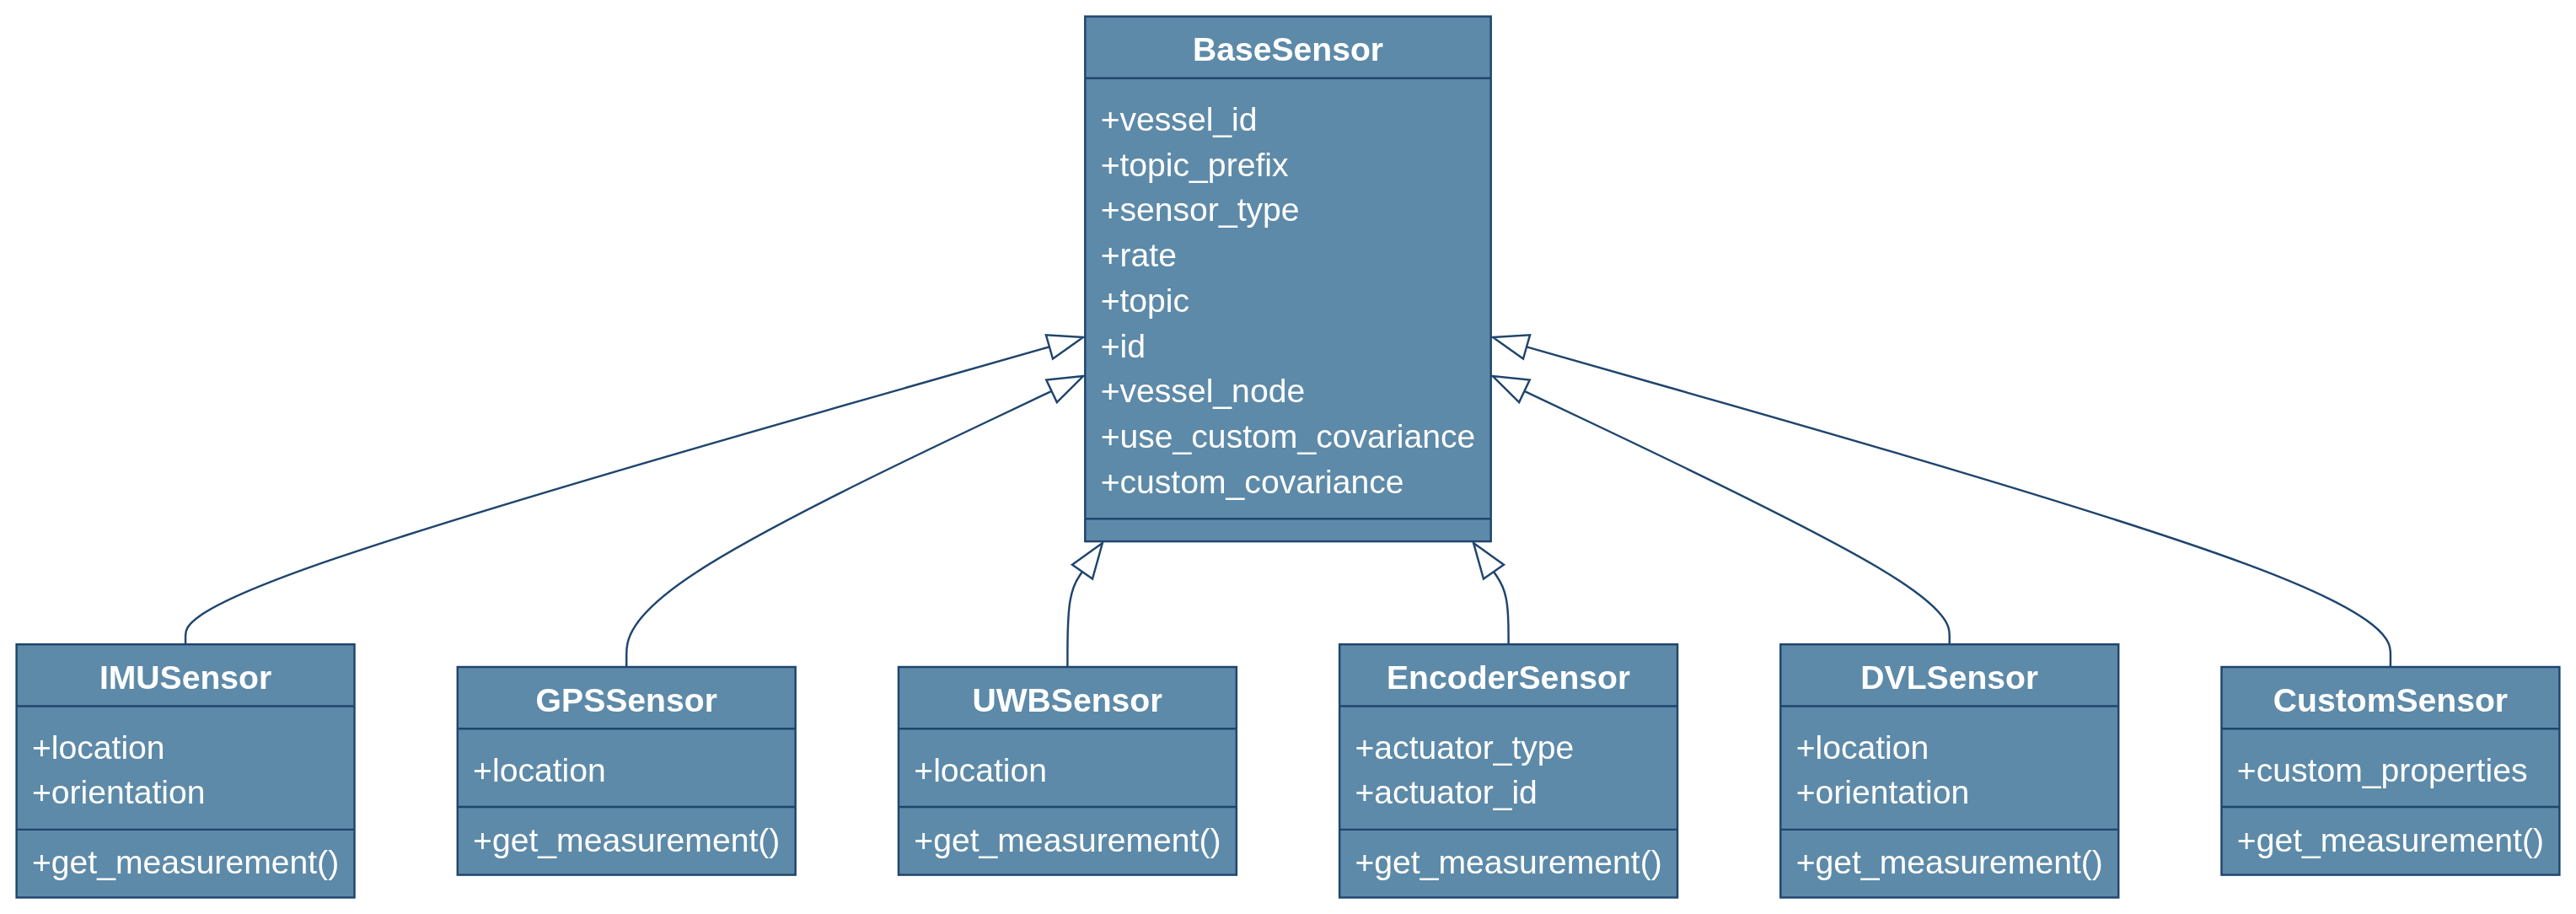
\includegraphics[width=13.02in,height=4.63in]{rawFiles/Navigation/sensors_files/figure-latex/mermaid-figure-1.png}

\section*{Sensor Types and
Simulation}\label{sensor-types-and-simulation}
\addcontentsline{toc}{section}{Sensor Types and Simulation}

\markright{Sensor Types and Simulation}

The simulator currently supports the following sensor types:

\subsection*{IMU (Inertial Measurement
Unit)}\label{imu-inertial-measurement-unit}
\addcontentsline{toc}{subsection}{IMU (Inertial Measurement Unit)}

IMU sensors measure:

\begin{itemize}
\tightlist
\item
  Orientation (quaternion)
\item
  Angular velocity (rad/s)
\item
  Linear acceleration (m/s²)
\end{itemize}

\textbf{Simulation details:}

The IMU simulation accounts for:

\begin{enumerate}
\def\labelenumi{\arabic{enumi}.}
\tightlist
\item
  Sensor placement relative to the vessel's center of mass
\item
  Sensor orientation relative to the vessel's body frame
\item
  Gravitational acceleration effects
\item
  Centripetal and tangential accelerations due to vessel rotation
\item
  Realistic noise models for all measurements
\end{enumerate}

\textbf{Noise model:}

\begin{itemize}
\tightlist
\item
  Orientation: Multivariate normal distribution applied to Euler angles
\item
  Angular velocity: Multivariate normal distribution
\item
  Linear acceleration: Multivariate normal distribution
\end{itemize}

The covariances are defined in the \texttt{sensors.yml} file.

\begin{Shaded}
\begin{Highlighting}[]
\CommentTok{\# Example of how IMU measurements are generated}
\KeywordTok{def}\NormalTok{ get\_measurement(}\VariableTok{self}\NormalTok{, quat}\OperatorTok{=}\VariableTok{False}\NormalTok{):}
\NormalTok{    state }\OperatorTok{=} \VariableTok{self}\NormalTok{.vessel\_node.vessel.current\_state}
\NormalTok{    state\_der }\OperatorTok{=} \VariableTok{self}\NormalTok{.vessel\_node.vessel.current\_state\_der}
    
    \CommentTok{\# Convert orientation and add noise}
\NormalTok{    q\_sensor }\OperatorTok{=}\NormalTok{ kin.rotm\_to\_quat(kin.quat\_to\_rotm(quat) }\OperatorTok{@}\NormalTok{ kin.quat\_to\_rotm(orientation\_quat))}
\NormalTok{    q\_sensor }\OperatorTok{=}\NormalTok{ kin.eul\_to\_quat(kin.quat\_to\_eul(q\_sensor) }\OperatorTok{+}\NormalTok{ np.random.multivariate\_normal(np.zeros(}\DecValTok{3}\NormalTok{), }\VariableTok{self}\NormalTok{.eul\_cov))}
    
    \CommentTok{\# Calculate acceleration including all effects}
\NormalTok{    acc\_bcs }\OperatorTok{=}\NormalTok{ state\_der[}\DecValTok{0}\NormalTok{:}\DecValTok{3}\NormalTok{] }\OperatorTok{+}\NormalTok{ np.cross(omg\_bcs, v\_bcs)}
\NormalTok{    acc\_s\_bcs }\OperatorTok{=}\NormalTok{ acc\_bcs }\OperatorTok{+}\NormalTok{ np.cross(alpha, }\VariableTok{self}\NormalTok{.location) }\OperatorTok{+}\NormalTok{ np.cross(omg\_bcs, np.cross(omg\_bcs, }\VariableTok{self}\NormalTok{.location))}
\NormalTok{    acc\_sensor }\OperatorTok{=}\NormalTok{ kin.quat\_to\_rotm(orientation\_quat).T }\OperatorTok{@}\NormalTok{ acc\_s\_bcs}
    
    \CommentTok{\# Add gravity and noise}
\NormalTok{    acc\_sensor }\OperatorTok{=}\NormalTok{ acc\_sensor }\OperatorTok{+}\NormalTok{ kin.quat\_to\_rotm(q\_sensor).T }\OperatorTok{@}\NormalTok{ np.array([}\DecValTok{0}\NormalTok{, }\DecValTok{0}\NormalTok{, }\OperatorTok{{-}}\VariableTok{self}\NormalTok{.vessel\_node.vessel.g])}
\NormalTok{    acc\_sensor }\OperatorTok{=}\NormalTok{ acc\_sensor }\OperatorTok{+}\NormalTok{ np.random.multivariate\_normal(np.zeros(}\DecValTok{3}\NormalTok{), }\VariableTok{self}\NormalTok{.lin\_acc\_cov)}

    \CommentTok{\# Calculate angular velocity with noise}
\NormalTok{    omg\_sensor }\OperatorTok{=}\NormalTok{ kin.quat\_to\_rotm(orientation\_quat).T }\OperatorTok{@}\NormalTok{ omg\_bcs}
\NormalTok{    omg\_sensor }\OperatorTok{=}\NormalTok{ omg\_sensor }\OperatorTok{+}\NormalTok{ np.random.multivariate\_normal(np.zeros(}\DecValTok{3}\NormalTok{), }\VariableTok{self}\NormalTok{.ang\_vel\_cov)}

    \ControlFlowTok{return}\NormalTok{ \{...\}  }\CommentTok{\# Return measurements and covariances}
\end{Highlighting}
\end{Shaded}

\subsection*{GPS (Global Positioning
System)}\label{gps-global-positioning-system}
\addcontentsline{toc}{subsection}{GPS (Global Positioning System)}

GPS sensors measure:

\begin{itemize}
\tightlist
\item
  Latitude (degrees)
\item
  Longitude (degrees)
\item
  Altitude (meters)
\end{itemize}

\textbf{Simulation details:}

The GPS simulation accounts for:

\begin{enumerate}
\def\labelenumi{\arabic{enumi}.}
\tightlist
\item
  Sensor placement on the vessel
\item
  Conversion between NED (North-East-Down) and LLH
  (Latitude-Longitude-Height) coordinates
\item
  Realistic position noise
\end{enumerate}

\textbf{Noise model:}

\begin{itemize}
\tightlist
\item
  Position: Multivariate normal distribution applied to NED coordinates
  before conversion to LLH
\end{itemize}

\begin{Shaded}
\begin{Highlighting}[]
\CommentTok{\# Example of how GPS measurements are generated}
\KeywordTok{def}\NormalTok{ get\_measurement(}\VariableTok{self}\NormalTok{, quat}\OperatorTok{=}\VariableTok{False}\NormalTok{):}
\NormalTok{    state }\OperatorTok{=} \VariableTok{self}\NormalTok{.vessel\_node.vessel.current\_state}
\NormalTok{    llh0 }\OperatorTok{=} \VariableTok{self}\NormalTok{.vessel\_node.vessel.gps\_datum}
    
    \CommentTok{\# Get position in NED, add sensor offset and noise}
\NormalTok{    ned }\OperatorTok{=}\NormalTok{ state[}\DecValTok{6}\NormalTok{:}\DecValTok{9}\NormalTok{] }\OperatorTok{+}\NormalTok{ kin.quat\_to\_rotm(orientation) }\OperatorTok{@} \VariableTok{self}\NormalTok{.location}
\NormalTok{    ned }\OperatorTok{=}\NormalTok{ ned }\OperatorTok{+}\NormalTok{ np.random.multivariate\_normal(np.zeros(}\DecValTok{3}\NormalTok{), }\VariableTok{self}\NormalTok{.gps\_cov)}
    
    \CommentTok{\# Convert to latitude{-}longitude{-}height}
\NormalTok{    llh }\OperatorTok{=}\NormalTok{ kin.ned\_to\_llh(ned, llh0)}

    \ControlFlowTok{return}\NormalTok{ \{...\}  }\CommentTok{\# Return latitude, longitude, altitude and covariance}
\end{Highlighting}
\end{Shaded}

\subsection*{UWB (Ultra-Wideband
Positioning)}\label{uwb-ultra-wideband-positioning}
\addcontentsline{toc}{subsection}{UWB (Ultra-Wideband Positioning)}

UWB sensors measure:

\begin{itemize}
\tightlist
\item
  Position in the NED frame (meters)
\end{itemize}

\textbf{Simulation details:}

The UWB simulation accounts for:

\begin{enumerate}
\def\labelenumi{\arabic{enumi}.}
\tightlist
\item
  Sensor placement on the vessel
\item
  Position in the NED coordinate frame
\item
  Realistic position noise (typically higher precision than GPS)
\end{enumerate}

\textbf{Noise model:}

\begin{itemize}
\tightlist
\item
  Position: Multivariate normal distribution applied to NED coordinates
\end{itemize}

\begin{Shaded}
\begin{Highlighting}[]
\CommentTok{\# Example of how UWB measurements are generated}
\KeywordTok{def}\NormalTok{ get\_measurement(}\VariableTok{self}\NormalTok{, quat}\OperatorTok{=}\VariableTok{False}\NormalTok{):}
\NormalTok{    state }\OperatorTok{=} \VariableTok{self}\NormalTok{.vessel\_node.vessel.current\_state}
\NormalTok{    ned }\OperatorTok{=}\NormalTok{ state[}\DecValTok{6}\NormalTok{:}\DecValTok{9}\NormalTok{]}
    
    \CommentTok{\# Get position and add sensor offset and noise}
\NormalTok{    r\_sen }\OperatorTok{=}\NormalTok{ ned }\OperatorTok{+}\NormalTok{ kin.quat\_to\_rotm(orientation) }\OperatorTok{@} \VariableTok{self}\NormalTok{.location}
\NormalTok{    r\_sen }\OperatorTok{=}\NormalTok{ r\_sen }\OperatorTok{+}\NormalTok{ np.random.multivariate\_normal(np.zeros(}\DecValTok{3}\NormalTok{), }\VariableTok{self}\NormalTok{.uwb\_cov)}

    \ControlFlowTok{return}\NormalTok{ \{...\}  }\CommentTok{\# Return position and covariance}
\end{Highlighting}
\end{Shaded}

\subsection*{Encoder Sensors}\label{encoder-sensors}
\addcontentsline{toc}{subsection}{Encoder Sensors}

Encoder sensors measure:

\begin{itemize}
\tightlist
\item
  Actuator position (degrees for control surfaces, RPM for thrusters)
\end{itemize}

\textbf{Simulation details:}

The encoder simulation accounts for:

\begin{enumerate}
\def\labelenumi{\arabic{enumi}.}
\tightlist
\item
  Specific actuator type (rudder, thruster, etc.)
\item
  Unit conversion from state vector to appropriate units
\item
  Actuator-specific noise characteristics
\end{enumerate}

\textbf{Noise model:}

\begin{itemize}
\tightlist
\item
  Actuator value: Normal distribution with specified RMS noise
\end{itemize}

\begin{Shaded}
\begin{Highlighting}[]
\CommentTok{\# Example of how Encoder measurements are generated}
\KeywordTok{def}\NormalTok{ get\_measurement(}\VariableTok{self}\NormalTok{):}
\NormalTok{    state }\OperatorTok{=} \VariableTok{self}\NormalTok{.vessel\_node.vessel.current\_state}
    
    \CommentTok{\# Get the specific actuator value from the state vector}
\NormalTok{    actuator\_value\_raw }\OperatorTok{=}\NormalTok{ state[}\VariableTok{self}\NormalTok{.state\_index]}
    
    \CommentTok{\# Apply unit conversion (e.g., rad to degrees, rad/s to RPM)}
\NormalTok{    actuator\_value\_converted }\OperatorTok{=}\NormalTok{ actuator\_value\_raw }\OperatorTok{*} \VariableTok{self}\NormalTok{.unit\_conversion}
    
    \CommentTok{\# Add noise to the converted measurement}
\NormalTok{    actuator\_value\_noisy }\OperatorTok{=}\NormalTok{ actuator\_value\_converted }\OperatorTok{+}\NormalTok{ np.random.normal(}\DecValTok{0}\NormalTok{, }\VariableTok{self}\NormalTok{.noise\_rms)}

    \ControlFlowTok{return}\NormalTok{ \{...\}  }\CommentTok{\# Return actuator value, name, and covariance}
\end{Highlighting}
\end{Shaded}

\subsection*{DVL (Doppler Velocity Log)}\label{dvl-doppler-velocity-log}
\addcontentsline{toc}{subsection}{DVL (Doppler Velocity Log)}

DVL sensors measure:

\begin{itemize}
\tightlist
\item
  Linear velocity in the body frame (m/s)
\end{itemize}

\textbf{Simulation details:}

The DVL simulation accounts for:

\begin{enumerate}
\def\labelenumi{\arabic{enumi}.}
\tightlist
\item
  Sensor placement and orientation
\item
  Body-frame velocity measurements
\item
  Realistic velocity noise
\end{enumerate}

\textbf{Noise model:}

\begin{itemize}
\tightlist
\item
  Velocity: Multivariate normal distribution applied to body-frame
  velocity
\end{itemize}

\begin{Shaded}
\begin{Highlighting}[]
\CommentTok{\# Example of how DVL measurements are generated}
\KeywordTok{def}\NormalTok{ get\_measurement(}\VariableTok{self}\NormalTok{, quat}\OperatorTok{=}\VariableTok{False}\NormalTok{):}
\NormalTok{    state }\OperatorTok{=} \VariableTok{self}\NormalTok{.vessel\_node.vessel.current\_state}
    
    \CommentTok{\# Get body{-}frame velocity and add noise}
\NormalTok{    v\_body }\OperatorTok{=}\NormalTok{ state[}\DecValTok{0}\NormalTok{:}\DecValTok{3}\NormalTok{]}
\NormalTok{    v\_body\_noisy }\OperatorTok{=}\NormalTok{ v\_body }\OperatorTok{+}\NormalTok{ np.random.multivariate\_normal(np.zeros(}\DecValTok{3}\NormalTok{), }\VariableTok{self}\NormalTok{.vel\_cov)}
    
    \ControlFlowTok{return}\NormalTok{ \{...\}  }\CommentTok{\# Return velocity and covariance}
\end{Highlighting}
\end{Shaded}

\section*{Sensor Configuration}\label{sensor-configuration}
\addcontentsline{toc}{section}{Sensor Configuration}

\markright{Sensor Configuration}

Sensors are configured through the YAML configuration files. Each sensor
definition includes:

\begin{itemize}
\tightlist
\item
  \textbf{sensor\_type}: The type of sensor (IMU, GPS, UWB, encoder,
  DVL)
\item
  \textbf{sensor\_topic}: ROS topic for publishing sensor data
\item
  \textbf{sensor\_location}: Position of the sensor in the body frame
  {[}x, y, z{]}
\item
  \textbf{sensor\_orientation}: Orientation of the sensor in the body
  frame {[}roll, pitch, yaw{]}
\item
  \textbf{publish\_rate}: Update frequency in Hz
\item
  \textbf{use\_custom\_covariance}: Boolean flag to use custom noise
  parameters
\item
  \textbf{custom\_covariance}: Custom noise covariance matrices for each
  measurement
\end{itemize}

Example configuration for an IMU sensor:

\begin{Shaded}
\begin{Highlighting}[]
\FunctionTok{sensors}\KeywordTok{:}
\AttributeTok{  }\KeywordTok{{-}}\AttributeTok{ }
\AttributeTok{    }\FunctionTok{sensor\_type}\KeywordTok{:}\AttributeTok{ IMU}
\AttributeTok{    }\FunctionTok{sensor\_topic}\KeywordTok{:}\AttributeTok{ /vessel\_01/imu/data}
\AttributeTok{    }\FunctionTok{sensor\_location}\KeywordTok{:}\AttributeTok{ }\KeywordTok{[}\FloatTok{0.0}\KeywordTok{,}\AttributeTok{ }\FloatTok{0.0}\KeywordTok{,}\AttributeTok{ }\FloatTok{0.1}\KeywordTok{]}
\AttributeTok{    }\FunctionTok{sensor\_orientation}\KeywordTok{:}\AttributeTok{ }\KeywordTok{[}\FloatTok{0.0}\KeywordTok{,}\AttributeTok{ }\FloatTok{0.0}\KeywordTok{,}\AttributeTok{ }\FloatTok{0.0}\KeywordTok{]}
\AttributeTok{    }\FunctionTok{publish\_rate}\KeywordTok{:}\AttributeTok{ }\DecValTok{100}
\AttributeTok{    }\FunctionTok{use\_custom\_covariance}\KeywordTok{:}\AttributeTok{ }\CharTok{true}
\AttributeTok{    }\FunctionTok{custom\_covariance}\KeywordTok{:}
\AttributeTok{      }\FunctionTok{orientation\_covariance}\KeywordTok{:}\AttributeTok{ }\KeywordTok{[}\FloatTok{0.001}\KeywordTok{,}\AttributeTok{ }\FloatTok{0.0}\KeywordTok{,}\AttributeTok{ }\FloatTok{0.0}\KeywordTok{,}\AttributeTok{ }\FloatTok{0.0}\KeywordTok{,}\AttributeTok{ }\FloatTok{0.001}\KeywordTok{,}\AttributeTok{ }\FloatTok{0.0}\KeywordTok{,}\AttributeTok{ }\FloatTok{0.0}\KeywordTok{,}\AttributeTok{ }\FloatTok{0.0}\KeywordTok{,}\AttributeTok{ }\FloatTok{0.001}\KeywordTok{]}
\AttributeTok{      }\FunctionTok{angular\_velocity\_covariance}\KeywordTok{:}\AttributeTok{ }\KeywordTok{[}\FloatTok{0.0001}\KeywordTok{,}\AttributeTok{ }\FloatTok{0.0}\KeywordTok{,}\AttributeTok{ }\FloatTok{0.0}\KeywordTok{,}\AttributeTok{ }\FloatTok{0.0}\KeywordTok{,}\AttributeTok{ }\FloatTok{0.0001}\KeywordTok{,}\AttributeTok{ }\FloatTok{0.0}\KeywordTok{,}\AttributeTok{ }\FloatTok{0.0}\KeywordTok{,}\AttributeTok{ }\FloatTok{0.0}\KeywordTok{,}\AttributeTok{ }\FloatTok{0.0001}\KeywordTok{]}
\AttributeTok{      }\FunctionTok{linear\_acceleration\_covariance}\KeywordTok{:}\AttributeTok{ }\KeywordTok{[}\FloatTok{0.01}\KeywordTok{,}\AttributeTok{ }\FloatTok{0.0}\KeywordTok{,}\AttributeTok{ }\FloatTok{0.0}\KeywordTok{,}\AttributeTok{ }\FloatTok{0.0}\KeywordTok{,}\AttributeTok{ }\FloatTok{0.01}\KeywordTok{,}\AttributeTok{ }\FloatTok{0.0}\KeywordTok{,}\AttributeTok{ }\FloatTok{0.0}\KeywordTok{,}\AttributeTok{ }\FloatTok{0.0}\KeywordTok{,}\AttributeTok{ }\FloatTok{0.01}\KeywordTok{]}
\end{Highlighting}
\end{Shaded}

\section*{Creating Custom Sensors}\label{creating-custom-sensors}
\addcontentsline{toc}{section}{Creating Custom Sensors}

\markright{Creating Custom Sensors}

To create your own custom sensor, follow these steps:

\subsection*{1. Create a new sensor
class}\label{create-a-new-sensor-class}
\addcontentsline{toc}{subsection}{1. Create a new sensor class}

Create a new class that inherits from \texttt{BaseSensor} and implements
the \texttt{get\_measurement()} method:

\begin{Shaded}
\begin{Highlighting}[]
\KeywordTok{class}\NormalTok{ CustomSensor(BaseSensor):}
    \KeywordTok{def} \FunctionTok{\_\_init\_\_}\NormalTok{(}\VariableTok{self}\NormalTok{, sensor\_config, vessel\_id, topic\_prefix, vessel\_node):}
        \BuiltInTok{super}\NormalTok{().}\FunctionTok{\_\_init\_\_}\NormalTok{(sensor\_config, vessel\_id, topic\_prefix, vessel\_node)}
        \CommentTok{\# Initialize sensor{-}specific properties}
        \VariableTok{self}\NormalTok{.location }\OperatorTok{=}\NormalTok{ np.array(sensor\_config[}\StringTok{\textquotesingle{}sensor\_location\textquotesingle{}}\NormalTok{])}
        \VariableTok{self}\NormalTok{.custom\_param }\OperatorTok{=}\NormalTok{ sensor\_config.get(}\StringTok{\textquotesingle{}custom\_param\textquotesingle{}}\NormalTok{, default\_value)}
        
        \CommentTok{\# Initialize noise parameters}
        \VariableTok{self}\NormalTok{.custom\_rms }\OperatorTok{=}\NormalTok{ np.array([}\FloatTok{0.1}\NormalTok{, }\FloatTok{0.1}\NormalTok{, }\FloatTok{0.1}\NormalTok{])}
        \VariableTok{self}\NormalTok{.custom\_cov }\OperatorTok{=}\NormalTok{ np.diag(}\VariableTok{self}\NormalTok{.custom\_rms }\OperatorTok{**} \DecValTok{2}\NormalTok{)}
        
        \CommentTok{\# Override with custom covariance if provided}
        \ControlFlowTok{if} \VariableTok{self}\NormalTok{.use\_custom\_covariance }\KeywordTok{and} \VariableTok{self}\NormalTok{.custom\_covariance:}
            \ControlFlowTok{if} \StringTok{\textquotesingle{}custom\_measurement\_covariance\textquotesingle{}} \KeywordTok{in} \VariableTok{self}\NormalTok{.custom\_covariance:}
                \VariableTok{self}\NormalTok{.custom\_cov }\OperatorTok{=}\NormalTok{ np.array(}\VariableTok{self}\NormalTok{.custom\_covariance[}\StringTok{\textquotesingle{}custom\_measurement\_covariance\textquotesingle{}}\NormalTok{]).reshape(}\DecValTok{3}\NormalTok{, }\DecValTok{3}\NormalTok{)}

    \KeywordTok{def}\NormalTok{ get\_measurement(}\VariableTok{self}\NormalTok{, quat}\OperatorTok{=}\VariableTok{False}\NormalTok{):}
        \CommentTok{\# Access vessel state}
\NormalTok{        state }\OperatorTok{=} \VariableTok{self}\NormalTok{.vessel\_node.vessel.current\_state}
        
        \CommentTok{\# Generate realistic measurements based on state}
        \CommentTok{\# Apply appropriate transformations, physics models, etc.}
        
        \CommentTok{\# Add noise to measurements}
\NormalTok{        measurement }\OperatorTok{=}\NormalTok{ calculated\_value }\OperatorTok{+}\NormalTok{ np.random.multivariate\_normal(np.zeros(}\DecValTok{3}\NormalTok{), }\VariableTok{self}\NormalTok{.custom\_cov)}
        
        \CommentTok{\# Return measurement as a dictionary}
        \ControlFlowTok{return}\NormalTok{ \{}
            \StringTok{\textquotesingle{}custom\_measurement\textquotesingle{}}\NormalTok{: measurement,}
            \StringTok{\textquotesingle{}covariance\textquotesingle{}}\NormalTok{: }\VariableTok{self}\NormalTok{.custom\_cov.flatten()}
\NormalTok{        \}}
\end{Highlighting}
\end{Shaded}

\subsection*{2. Register your sensor in the factory
function}\label{register-your-sensor-in-the-factory-function}
\addcontentsline{toc}{subsection}{2. Register your sensor in the factory
function}

Modify the \texttt{create\_sensor} function to include your new sensor
type:

\begin{Shaded}
\begin{Highlighting}[]
\KeywordTok{def}\NormalTok{ create\_sensor(sensor\_config, vessel\_id, topic\_prefix, vessel\_node):}
    \CommentTok{"""Factory function to create appropriate sensor object based on sensor type"""}
\NormalTok{    sensor\_type }\OperatorTok{=}\NormalTok{ sensor\_config[}\StringTok{\textquotesingle{}sensor\_type\textquotesingle{}}\NormalTok{]}
\NormalTok{    sensor\_classes }\OperatorTok{=}\NormalTok{ \{}
        \StringTok{\textquotesingle{}IMU\textquotesingle{}}\NormalTok{: IMUSensor,}
        \StringTok{\textquotesingle{}GPS\textquotesingle{}}\NormalTok{: GPSSensor,}
        \StringTok{\textquotesingle{}UWB\textquotesingle{}}\NormalTok{: UWBSensor,}
        \StringTok{\textquotesingle{}encoder\textquotesingle{}}\NormalTok{: EncoderSensor,}
        \StringTok{\textquotesingle{}DVL\textquotesingle{}}\NormalTok{: DVLSensor,}
        \StringTok{\textquotesingle{}CustomSensor\textquotesingle{}}\NormalTok{: CustomSensor  }\CommentTok{\# Add your custom sensor here}
\NormalTok{    \}}
    
    \ControlFlowTok{if}\NormalTok{ sensor\_type }\KeywordTok{not} \KeywordTok{in}\NormalTok{ sensor\_classes:}
        \ControlFlowTok{raise} \PreprocessorTok{ValueError}\NormalTok{(}\SpecialStringTok{f"Unknown sensor type: }\SpecialCharTok{\{}\NormalTok{sensor\_type}\SpecialCharTok{\}}\SpecialStringTok{"}\NormalTok{)}
        
    \ControlFlowTok{return}\NormalTok{ sensor\_classes[sensor\_type](sensor\_config, vessel\_id, topic\_prefix, vessel\_node)}
\end{Highlighting}
\end{Shaded}

\subsection*{3. Create a ROS publisher for your custom
sensor}\label{create-a-ros-publisher-for-your-custom-sensor}
\addcontentsline{toc}{subsection}{3. Create a ROS publisher for your
custom sensor}

In your vessel's ROS node, add a publisher for your custom sensor:

\begin{Shaded}
\begin{Highlighting}[]
\CommentTok{\# In the vessel ROS node initialization}
\ControlFlowTok{if}\NormalTok{ sensor.sensor\_type }\OperatorTok{==} \StringTok{\textquotesingle{}CustomSensor\textquotesingle{}}\NormalTok{:}
    \CommentTok{\# Create a publisher for your custom sensor}
    \CommentTok{\# Choose an appropriate message type or create a custom one}
    \ImportTok{from}\NormalTok{ your\_package.msg }\ImportTok{import}\NormalTok{ CustomSensorMsg}
    
\NormalTok{    publisher }\OperatorTok{=} \VariableTok{self}\NormalTok{.create\_publisher(}
\NormalTok{        CustomSensorMsg,}
        \SpecialStringTok{f\textquotesingle{}}\SpecialCharTok{\{}\VariableTok{self}\SpecialCharTok{.}\NormalTok{topic\_prefix}\SpecialCharTok{\}}\SpecialStringTok{/}\SpecialCharTok{\{}\NormalTok{sensor}\SpecialCharTok{.}\NormalTok{topic}\SpecialCharTok{\}}\SpecialStringTok{\textquotesingle{}}\NormalTok{,}
        \DecValTok{10}
\NormalTok{    )}
    
    \CommentTok{\# Add the publisher to the sensor publishers dictionary}
    \VariableTok{self}\NormalTok{.sensor\_publishers[sensor] }\OperatorTok{=}\NormalTok{ publisher}
    
\CommentTok{\# In the vessel ROS node update method}
\ControlFlowTok{if}\NormalTok{ sensor.sensor\_type }\OperatorTok{==} \StringTok{\textquotesingle{}CustomSensor\textquotesingle{}}\NormalTok{:}
    \CommentTok{\# Create a message for your custom sensor}
\NormalTok{    msg }\OperatorTok{=}\NormalTok{ CustomSensorMsg()}
    
    \CommentTok{\# Fill the message with sensor data}
\NormalTok{    measurement }\OperatorTok{=}\NormalTok{ sensor.get\_measurement()}
\NormalTok{    msg.data }\OperatorTok{=}\NormalTok{ measurement[}\StringTok{\textquotesingle{}custom\_measurement\textquotesingle{}}\NormalTok{]}
\NormalTok{    msg.covariance }\OperatorTok{=}\NormalTok{ measurement[}\StringTok{\textquotesingle{}covariance\textquotesingle{}}\NormalTok{]}
    
    \CommentTok{\# Add a timestamp}
\NormalTok{    msg.header.stamp }\OperatorTok{=} \VariableTok{self}\NormalTok{.get\_clock().now().to\_msg()}
    
    \CommentTok{\# Publish the message}
    \VariableTok{self}\NormalTok{.sensor\_publishers[sensor].publish(msg)}
\end{Highlighting}
\end{Shaded}

\subsection*{4. Configure your custom sensor in the YAML
file}\label{configure-your-custom-sensor-in-the-yaml-file}
\addcontentsline{toc}{subsection}{4. Configure your custom sensor in the
YAML file}

Add your custom sensor to the sensors configuration file:

\begin{Shaded}
\begin{Highlighting}[]
\FunctionTok{sensors}\KeywordTok{:}
\AttributeTok{  }\KeywordTok{{-}}\AttributeTok{ }
\AttributeTok{    }\FunctionTok{sensor\_type}\KeywordTok{:}\AttributeTok{ CustomSensor}
\AttributeTok{    }\FunctionTok{sensor\_topic}\KeywordTok{:}\AttributeTok{ /vessel\_01/custom\_sensor}
\AttributeTok{    }\FunctionTok{sensor\_location}\KeywordTok{:}\AttributeTok{ }\KeywordTok{[}\FloatTok{0.1}\KeywordTok{,}\AttributeTok{ }\FloatTok{0.0}\KeywordTok{,}\AttributeTok{ }\FloatTok{0.2}\KeywordTok{]}
\AttributeTok{    }\FunctionTok{sensor\_orientation}\KeywordTok{:}\AttributeTok{ }\KeywordTok{[}\FloatTok{0.0}\KeywordTok{,}\AttributeTok{ }\FloatTok{0.0}\KeywordTok{,}\AttributeTok{ }\FloatTok{0.0}\KeywordTok{]}
\AttributeTok{    }\FunctionTok{publish\_rate}\KeywordTok{:}\AttributeTok{ }\DecValTok{50}
\AttributeTok{    }\FunctionTok{custom\_param}\KeywordTok{:}\AttributeTok{ }\FloatTok{42.0}
\AttributeTok{    }\FunctionTok{use\_custom\_covariance}\KeywordTok{:}\AttributeTok{ }\CharTok{true}
\AttributeTok{    }\FunctionTok{custom\_covariance}\KeywordTok{:}
\AttributeTok{      }\FunctionTok{custom\_measurement\_covariance}\KeywordTok{:}\AttributeTok{ }\KeywordTok{[}\FloatTok{0.01}\KeywordTok{,}\AttributeTok{ }\FloatTok{0.0}\KeywordTok{,}\AttributeTok{ }\FloatTok{0.0}\KeywordTok{,}\AttributeTok{ }\FloatTok{0.0}\KeywordTok{,}\AttributeTok{ }\FloatTok{0.01}\KeywordTok{,}\AttributeTok{ }\FloatTok{0.0}\KeywordTok{,}\AttributeTok{ }\FloatTok{0.0}\KeywordTok{,}\AttributeTok{ }\FloatTok{0.0}\KeywordTok{,}\AttributeTok{ }\FloatTok{0.01}\KeywordTok{]}
\end{Highlighting}
\end{Shaded}

\section*{Best Practices for Sensor
Simulation}\label{best-practices-for-sensor-simulation}
\addcontentsline{toc}{section}{Best Practices for Sensor Simulation}

\markright{Best Practices for Sensor Simulation}

When working with sensors in the simulator, follow these guidelines:

\begin{enumerate}
\def\labelenumi{\arabic{enumi}.}
\item
  \textbf{Physical realism}:

  \begin{itemize}
  \tightlist
  \item
    Place sensors at realistic positions on the vessel
  \item
    Use realistic noise parameters based on actual sensor specifications
  \item
    Consider environmental effects if appropriate (e.g., GPS degradation
    underwater)
  \end{itemize}
\item
  \textbf{Computational efficiency}:

  \begin{itemize}
  \tightlist
  \item
    Set appropriate update rates based on real-world sensors
  \item
    Use optimized noise generation methods for high-frequency sensors
  \end{itemize}
\item
  \textbf{Sensor fusion testing}:

  \begin{itemize}
  \tightlist
  \item
    Configure multiple sensor types to test fusion algorithms
  \item
    Vary noise parameters to test robustness of estimation algorithms
  \end{itemize}
\item
  \textbf{Custom sensors}:

  \begin{itemize}
  \tightlist
  \item
    Follow the class structure of existing sensors
  \item
    Document physical models and assumptions clearly
  \item
    Use appropriate coordinate transformations
  \end{itemize}
\item
  \textbf{Topic naming}:

  \begin{itemize}
  \tightlist
  \item
    Use consistent naming conventions for sensors
  \item
    Include vessel ID in topic names for multi-vessel simulations
  \end{itemize}
\end{enumerate}

\bookmarksetup{startatroot}

\chapter*{Simualtion Inputs}\label{simualtion-inputs}
\addcontentsline{toc}{chapter}{Simualtion Inputs}

\markboth{Simualtion Inputs}{Simualtion Inputs}

\section*{Overview}\label{overview-4}
\addcontentsline{toc}{section}{Overview}

\markright{Overview}

The Panisim simulator uses a structured set of YAML configuration files
to define all aspects of the simulation environment, vessel properties,
sensor configurations and guidance. This modular approach allows for
easy customization and extension of simulation scenarios without
modifying the core simulation code. The input files are auto generated
via the interactive Web GUI, but can also be modified manually.

\begin{tcolorbox}[enhanced jigsaw, colback=white, toptitle=1mm, colframe=quarto-callout-tip-color-frame, rightrule=.15mm, breakable, title=\textcolor{quarto-callout-tip-color}{\faLightbulb}\hspace{0.5em}{Tip}, toprule=.15mm, opacitybacktitle=0.6, opacityback=0, coltitle=black, leftrule=.75mm, colbacktitle=quarto-callout-tip-color!10!white, arc=.35mm, titlerule=0mm, bottomtitle=1mm, bottomrule=.15mm, left=2mm]

All input files follow the YAML format, which is human-readable and easy
to edit.

\end{tcolorbox}

\section*{Input File Structure}\label{input-file-structure}
\addcontentsline{toc}{section}{Input File Structure}

\markright{Input File Structure}

The input file system follows a hierarchical structure (zoom in to see
the chart more clearly).

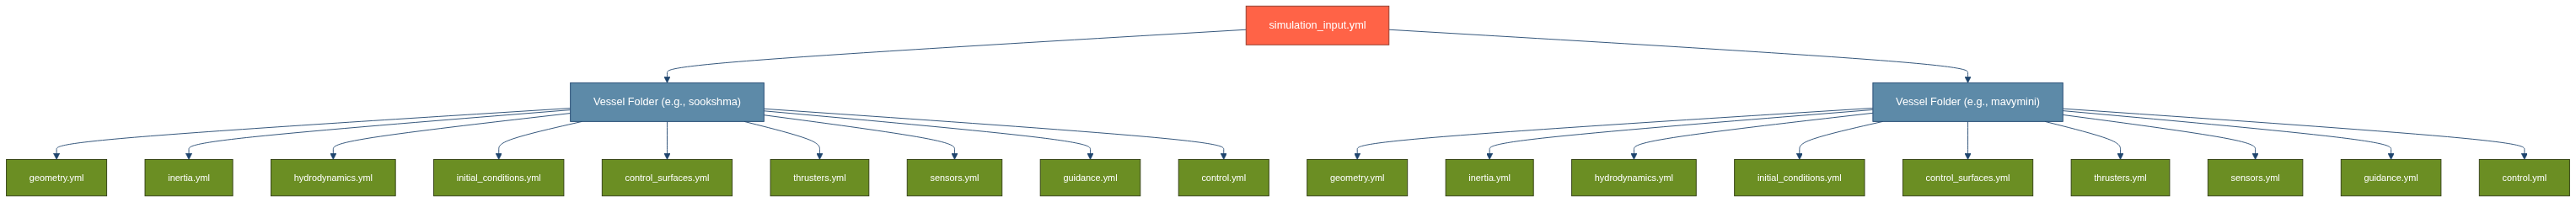
\includegraphics[width=35.06in,height=2.77in]{rawFiles/Inputs/inputs_files/figure-latex/mermaid-figure-1.png}

The top-level \texttt{simulation\_input.yml} file defines global
simulation parameters and references vessel-specific configuration files
stored in separate folders (one for each vessel type).

\section*{Main Configuration File}\label{main-configuration-file}
\addcontentsline{toc}{section}{Main Configuration File}

\markright{Main Configuration File}

The \texttt{simulation\_input.yml} file is the entry point for the
simulator configuration. It specifies global parameters and the list of
agents (vessels) to include in the simulation.

Example structure:

\begin{Shaded}
\begin{Highlighting}[]
\FunctionTok{sim\_time}\KeywordTok{:}\AttributeTok{ }\FloatTok{100.0}\CommentTok{               \# Total simulation time in seconds}
\FunctionTok{time\_step}\KeywordTok{:}\AttributeTok{ }\FloatTok{0.01}\CommentTok{               \# Simulation time step in seconds}
\FunctionTok{density}\KeywordTok{:}\AttributeTok{ }\FloatTok{1025.0}\CommentTok{               \# Water density (kg/m³)}
\FunctionTok{gravity}\KeywordTok{:}\AttributeTok{ }\FloatTok{9.80665}\CommentTok{              \# Gravitational acceleration (m/s²)}
\FunctionTok{world\_size}\KeywordTok{:}\AttributeTok{ }\KeywordTok{[}\DecValTok{1000}\KeywordTok{,}\AttributeTok{ }\DecValTok{1000}\KeywordTok{,}\AttributeTok{ }\DecValTok{100}\KeywordTok{]}\CommentTok{ \# Simulation world dimensions [x, y, z] in meters}
\FunctionTok{gps\_datum}\KeywordTok{:}\AttributeTok{ }\KeywordTok{[}\FloatTok{13.06}\KeywordTok{,}\AttributeTok{ }\FloatTok{80.28}\KeywordTok{,}\AttributeTok{ }\DecValTok{0}\KeywordTok{]}\CommentTok{  \# GPS reference point [latitude, longitude, height]}
\FunctionTok{nagents}\KeywordTok{:}\AttributeTok{ }\DecValTok{1}\CommentTok{                    \# Number of agents in the simulation}
\FunctionTok{geofence}\KeywordTok{:}\AttributeTok{ }\KeywordTok{[]}\CommentTok{                  \# Optional geofencing boundaries}

\FunctionTok{agents}\KeywordTok{:}
\AttributeTok{  }\KeywordTok{{-}}\AttributeTok{ }\FunctionTok{name}\KeywordTok{:}\AttributeTok{ }\StringTok{"sookshma"}\CommentTok{          \# Vessel name}
\AttributeTok{    }\FunctionTok{type}\KeywordTok{:}\AttributeTok{ }\StringTok{"usv"}\CommentTok{               \# Vessel type (usv, auv, etc.)}
\AttributeTok{    }\FunctionTok{active\_dof}\KeywordTok{:}\AttributeTok{ }\KeywordTok{[}\DecValTok{1}\KeywordTok{,}\AttributeTok{ }\DecValTok{1}\KeywordTok{,}\AttributeTok{ }\DecValTok{0}\KeywordTok{,}\AttributeTok{ }\DecValTok{0}\KeywordTok{,}\AttributeTok{ }\DecValTok{0}\KeywordTok{,}\AttributeTok{ }\DecValTok{1}\KeywordTok{]}\CommentTok{  \# Active degrees of freedom [u, v, w, p, q, r]}
\AttributeTok{    }\FunctionTok{U}\KeywordTok{:}\AttributeTok{ }\FloatTok{0.0}\CommentTok{                    \# Initial forward speed}
\AttributeTok{    }\FunctionTok{maintain\_speed}\KeywordTok{:}\AttributeTok{ }\CharTok{false}\CommentTok{     \# Whether to maintain constant forward speed}
\AttributeTok{    }
\CommentTok{    \# Paths to configuration files (relative or absolute)}
\CommentTok{    \# \{name\} will be replaced with the vessel name}
\AttributeTok{    }\FunctionTok{geometry}\KeywordTok{:}\AttributeTok{ }\StringTok{"inputs/\{name\}/geometry.yml"}
\AttributeTok{    }\FunctionTok{inertia}\KeywordTok{:}\AttributeTok{ }\StringTok{"inputs/\{name\}/inertia.yml"}
\AttributeTok{    }\FunctionTok{hydrodynamics}\KeywordTok{:}\AttributeTok{ }\StringTok{"inputs/\{name\}/hydrodynamics.yml"}
\AttributeTok{    }\FunctionTok{control\_surfaces}\KeywordTok{:}\AttributeTok{ }\StringTok{"inputs/\{name\}/control\_surfaces.yml"}
\AttributeTok{    }\FunctionTok{thrusters}\KeywordTok{:}\AttributeTok{ }\StringTok{"inputs/\{name\}/thrusters.yml"}
\AttributeTok{    }\FunctionTok{initial\_conditions}\KeywordTok{:}\AttributeTok{ }\StringTok{"inputs/\{name\}/initial\_conditions.yml"}
\AttributeTok{    }\FunctionTok{sensors}\KeywordTok{:}\AttributeTok{ }\StringTok{"inputs/\{name\}/sensors.yml"}
\AttributeTok{    }\FunctionTok{guidance}\KeywordTok{:}\AttributeTok{ }\StringTok{"inputs/\{name\}/guidance.yml"}
\AttributeTok{    }\FunctionTok{control}\KeywordTok{:}\AttributeTok{ }\StringTok{"inputs/\{name\}/control.yml"}
\end{Highlighting}
\end{Shaded}

\subsection*{Key Parameters}\label{key-parameters}
\addcontentsline{toc}{subsection}{Key Parameters}

\begin{longtable}[]{@{}
  >{\raggedright\arraybackslash}p{(\linewidth - 4\tabcolsep) * \real{0.3548}}
  >{\raggedright\arraybackslash}p{(\linewidth - 4\tabcolsep) * \real{0.4194}}
  >{\raggedright\arraybackslash}p{(\linewidth - 4\tabcolsep) * \real{0.2258}}@{}}
\toprule\noalign{}
\begin{minipage}[b]{\linewidth}\raggedright
Parameter
\end{minipage} & \begin{minipage}[b]{\linewidth}\raggedright
Description
\end{minipage} & \begin{minipage}[b]{\linewidth}\raggedright
Units
\end{minipage} \\
\midrule\noalign{}
\endhead
\bottomrule\noalign{}
\endlastfoot
\texttt{sim\_time} & Total simulation duration & seconds \\
\texttt{time\_step} & Simulation time step size & seconds \\
\texttt{density} & Water density & kg/m³ \\
\texttt{gravity} & Gravitational acceleration & m/s² \\
\texttt{world\_size} & Simulation world dimensions {[}x, y, z{]} &
meters \\
\texttt{gps\_datum} & Reference point for GPS coordinates {[}lat, lon,
height{]} & degrees, degrees, meters \\
\texttt{nagents} & Number of agents (vessels) in the simulation &
integer \\
\texttt{geofence} & Optional boundaries for the simulation area &
meters \\
\end{longtable}

\subsection*{Agent Configuration}\label{agent-configuration}
\addcontentsline{toc}{subsection}{Agent Configuration}

Each agent (vessel) in the \texttt{agents} list requires:

\begin{itemize}
\tightlist
\item
  \texttt{name}: Identifier for the vessel, used for file path
  resolution
\item
  \texttt{type}: Type of vessel (``usv'', ``auv'', etc.)
\item
  \texttt{active\_dof}: Array of 6 binary values indicating which
  degrees of freedom are active {[}surge, sway, heave, roll, pitch,
  yaw{]}
\item
  \texttt{U}: Initial/desired forward speed
\item
  \texttt{maintain\_speed}: Boolean flag to maintain constant forward
  speed
\end{itemize}

File paths can be absolute or relative (although we would recommend
using the same folder structure as the default). The special placeholder
\texttt{\{name\}} will be replaced with the vessel name, allowing for a
standardized folder structure.

\section*{Vessel-Specific Configuration
Files}\label{vessel-specific-configuration-files}
\addcontentsline{toc}{section}{Vessel-Specific Configuration Files}

\markright{Vessel-Specific Configuration Files}

Each vessel has its own set of configuration files that define its
physical properties, sensors, and control elements. This is defined in a
folder named after the vessel.

\subsection*{\texorpdfstring{Geometry Configuration
(\texttt{geometry.yml})}{Geometry Configuration (geometry.yml)}}\label{geometry-configuration-geometry.yml}
\addcontentsline{toc}{subsection}{Geometry Configuration
(\texttt{geometry.yml})}

The geometry file defines the vessel's physical dimensions and
coordinate frames.

Example from sookshma:

\begin{Shaded}
\begin{Highlighting}[]
\CommentTok{\# Dimensions of the box enclosing the vessel}
\FunctionTok{length}\KeywordTok{:}\AttributeTok{ }\DecValTok{1}
\FunctionTok{breadth}\KeywordTok{:}\AttributeTok{ }\FloatTok{0.24}
\FunctionTok{depth}\KeywordTok{:}\AttributeTok{ }\FloatTok{0.5}
\FunctionTok{Fn}\KeywordTok{:}\AttributeTok{ }\FloatTok{0.16}
\FunctionTok{gyration}\KeywordTok{:}\AttributeTok{ }\KeywordTok{[}\FloatTok{0.096}\KeywordTok{,}\AttributeTok{ }\FloatTok{0.25}\KeywordTok{,}\AttributeTok{ }\FloatTok{0.25}\KeywordTok{]}
\FunctionTok{CO}\KeywordTok{:}
\AttributeTok{  }\FunctionTok{position}\KeywordTok{:}\AttributeTok{ }\KeywordTok{[}\FloatTok{0.0}\KeywordTok{,}\AttributeTok{ }\FloatTok{0.0}\KeywordTok{,}\AttributeTok{ }\FloatTok{0.0}\KeywordTok{]}\CommentTok{ \# Relative to the origin of the 3d software}
\AttributeTok{  }\FunctionTok{orientation}\KeywordTok{:}\AttributeTok{ }\KeywordTok{[}\FloatTok{0.0}\KeywordTok{,}\AttributeTok{ }\FloatTok{0.0}\KeywordTok{,}\AttributeTok{ }\FloatTok{0.0}\KeywordTok{]}
\FunctionTok{CG}\KeywordTok{:}
\AttributeTok{  }\FunctionTok{position}\KeywordTok{:}\AttributeTok{ }\KeywordTok{[}\FloatTok{2.89415958e{-}02}\KeywordTok{,}\AttributeTok{ }\FloatTok{0.0}\KeywordTok{,}\AttributeTok{ }\FloatTok{1.62558889e{-}01}\KeywordTok{]}
\FunctionTok{CB}\KeywordTok{:}
\AttributeTok{  }\FunctionTok{position}\KeywordTok{:}\AttributeTok{ }\KeywordTok{[}\FloatTok{2.89415958e{-}02}\KeywordTok{,}\AttributeTok{ }\FloatTok{0.0}\KeywordTok{,}\AttributeTok{ }\FloatTok{1.36000000e{-}01}\KeywordTok{]}
\AttributeTok{  }
\FunctionTok{geometry\_file}\KeywordTok{:}\AttributeTok{ /workspaces/mavlab/inputs/sookshma/HydRA/input/sookshma.gdf}
\end{Highlighting}
\end{Shaded}

\subsubsection*{Key Parameters}\label{key-parameters-1}
\addcontentsline{toc}{subsubsection}{Key Parameters}

\begin{longtable}[]{@{}lll@{}}
\toprule\noalign{}
Parameter & Description & Units \\
\midrule\noalign{}
\endhead
\bottomrule\noalign{}
\endlastfoot
\texttt{length} & Overall length & meters \\
\texttt{breadth} & Overall width & meters \\
\texttt{depth} & Overall depth & meters \\
\texttt{Fn} & Froude number & dimensionless \\
\texttt{gyration} & Gyration radii {[}x, y, z{]} & meters \\
\texttt{CO} & Coordinate origin position and orientation & meters,
radians \\
\texttt{CG} & Center of gravity position and orientation & meters,
radians \\
\texttt{CB} & Center of buoyancy position and orientation & meters,
radians \\
\texttt{geometry\_file} & Path to 3D geometry file & string \\
\end{longtable}

\subsection*{\texorpdfstring{Inertia Configuration
(\texttt{inertia.yml})}{Inertia Configuration (inertia.yml)}}\label{inertia-configuration-inertia.yml}
\addcontentsline{toc}{subsection}{Inertia Configuration
(\texttt{inertia.yml})}

The inertia file defines the vessel's mass properties.

Example from sookshma:

\begin{Shaded}
\begin{Highlighting}[]
\FunctionTok{mass}\KeywordTok{:}\AttributeTok{ }\FloatTok{7.65}\CommentTok{ \# in kg}
\FunctionTok{buoyancy\_mass}\KeywordTok{:}\AttributeTok{ }\FloatTok{7.65}\CommentTok{ \# in kg}
\FunctionTok{inertia\_matrix}\KeywordTok{:}\AttributeTok{ None}\CommentTok{ \# in kg*m\^{}2}
\FunctionTok{added\_mass\_matrix}\KeywordTok{:}\AttributeTok{ None}\CommentTok{ \# in kg*m\^{}2/s}
\end{Highlighting}
\end{Shaded}

\subsubsection*{Key Parameters}\label{key-parameters-2}
\addcontentsline{toc}{subsubsection}{Key Parameters}

\begin{longtable}[]{@{}
  >{\raggedright\arraybackslash}p{(\linewidth - 4\tabcolsep) * \real{0.3548}}
  >{\raggedright\arraybackslash}p{(\linewidth - 4\tabcolsep) * \real{0.4194}}
  >{\raggedright\arraybackslash}p{(\linewidth - 4\tabcolsep) * \real{0.2258}}@{}}
\toprule\noalign{}
\begin{minipage}[b]{\linewidth}\raggedright
Parameter
\end{minipage} & \begin{minipage}[b]{\linewidth}\raggedright
Description
\end{minipage} & \begin{minipage}[b]{\linewidth}\raggedright
Units
\end{minipage} \\
\midrule\noalign{}
\endhead
\bottomrule\noalign{}
\endlastfoot
\texttt{mass} & Vessel mass & kg \\
\texttt{buoyancy\_mass} & Mass of displaced fluid (for neutral buoyancy,
equal to mass) & kg \\
\texttt{inertia\_matrix} & Optional explicit inertia matrix needs to be
6x6 (example:
\texttt{{[}{[}1,\ 0,\ 0,\ 0,\ 0,\ 0{]},\ {[}0,\ 1,\ 0,\ 0,\ 0,\ 0{]},\ {[}0,\ 0,\ 1,\ 0,\ 0,\ 0{]},\ {[}0,\ 0,\ 0,\ 1,\ 0,\ 0{]},\ {[}0,\ 0,\ 0,\ 0,\ 1,\ 0{]},\ {[}0,\ 0,\ 0,\ 0,\ 0,\ 1{]}{]}})
& kg·m² \\
\texttt{added\_mass\_matrix} & Optional explicit added mass matrix needs
to be 6x6 & kg, kg·m², kg·m \\
\end{longtable}

If the inertia matrix is not provided, it is calculated using the
gyration radii and the mass via the \texttt{\_generate\_mass\_matrix()}
function in the \texttt{calculate\_hydrodynamics.py} module. If the
added mass matrix is not provided, it will be calculated either using
the hydrodynamic derivatives or using the hydrodynamic coefficients from
the HydRA model.

\subsection*{\texorpdfstring{Hydrodynamics Configuration
(\texttt{hydrodynamics.yml})}{Hydrodynamics Configuration (hydrodynamics.yml)}}\label{hydrodynamics-configuration-hydrodynamics.yml}
\addcontentsline{toc}{subsection}{Hydrodynamics Configuration
(\texttt{hydrodynamics.yml})}

The hydrodynamics file contains coefficients for damping forces and
added mass.

Example from sookshma:

\begin{Shaded}
\begin{Highlighting}[]
\FunctionTok{hydra\_file}\KeywordTok{:}\AttributeTok{ /workspaces/mavlab/inputs/sookshma/HydRA/matlab/sookshma\_hydra.json}
\FunctionTok{dim\_flag}\KeywordTok{:}\AttributeTok{ }\CharTok{false}
\FunctionTok{cross\_flow\_drag}\KeywordTok{:}\AttributeTok{ }\CharTok{false}
\FunctionTok{coriolis\_flag}\KeywordTok{:}\AttributeTok{ }\CharTok{false}\CommentTok{ \# For linear dynamic model}

\CommentTok{\# Surge hydrodynamic derivatives}
\FunctionTok{X\_u}\KeywordTok{:}\AttributeTok{ }\FloatTok{{-}0.01}

\CommentTok{\# Sway hydrodynamic derivatives}
\FunctionTok{Y\_v}\KeywordTok{:}\AttributeTok{ }\FloatTok{{-}0.010659050686665396}
\FunctionTok{Y\_r}\KeywordTok{:}\AttributeTok{ }\FloatTok{0.0017799664706713543}

\CommentTok{\# Yaw hydrodynamic derivatives}
\FunctionTok{N\_v}\KeywordTok{:}\AttributeTok{ }\FloatTok{{-}0.0006242757399292063}
\FunctionTok{N\_r}\KeywordTok{:}\AttributeTok{ }\FloatTok{{-}0.001889456681929024}
\end{Highlighting}
\end{Shaded}

\subsubsection*{Key Parameters}\label{key-parameters-3}
\addcontentsline{toc}{subsubsection}{Key Parameters}

\begin{longtable}[]{@{}
  >{\raggedright\arraybackslash}p{(\linewidth - 4\tabcolsep) * \real{0.3548}}
  >{\raggedright\arraybackslash}p{(\linewidth - 4\tabcolsep) * \real{0.4194}}
  >{\raggedright\arraybackslash}p{(\linewidth - 4\tabcolsep) * \real{0.2258}}@{}}
\toprule\noalign{}
\begin{minipage}[b]{\linewidth}\raggedright
Parameter
\end{minipage} & \begin{minipage}[b]{\linewidth}\raggedright
Description
\end{minipage} & \begin{minipage}[b]{\linewidth}\raggedright
Units
\end{minipage} \\
\midrule\noalign{}
\endhead
\bottomrule\noalign{}
\endlastfoot
\texttt{hydra\_file} & Path to HydRA data file & string \\
\texttt{dim\_flag} & Whether coefficients are dimensional (true) or
non-dimensional (false) & boolean \\
\texttt{cross\_flow\_drag} & Whether to use cross-flow drag calculation
& boolean \\
\texttt{coriolis\_flag} & Whether to include Coriolis forces &
boolean \\
\end{longtable}

You can enter any combination of the hydrodynamic coefficients, and
it'll be handled by the simulator. They should be separated by
underscores. For example, \texttt{X\_u\_u} or \texttt{M\_r\_r}.

\subsection*{\texorpdfstring{Control Surfaces Configuration
(\texttt{control\_surfaces.yml})}{Control Surfaces Configuration (control\_surfaces.yml)}}\label{control-surfaces-configuration-control_surfaces.yml}
\addcontentsline{toc}{subsection}{Control Surfaces Configuration
(\texttt{control\_surfaces.yml})}

This file defines the vessel's control surfaces such as rudders, fins,
or foils.

Example from sookshma:

\begin{Shaded}
\begin{Highlighting}[]
\FunctionTok{naca\_number}\KeywordTok{:}\AttributeTok{ }\OtherTok{\&naca}\AttributeTok{ None}
\FunctionTok{naca\_file}\KeywordTok{:}\AttributeTok{ }\OtherTok{\&naca\_file}\AttributeTok{ None}
\FunctionTok{delta\_max}\KeywordTok{:}\AttributeTok{ }\OtherTok{\&dmax}\AttributeTok{ 35.0}
\FunctionTok{deltad\_max}\KeywordTok{:}\AttributeTok{ }\OtherTok{\&ddmax}\AttributeTok{ 1.0}
\FunctionTok{area}\KeywordTok{:}\AttributeTok{ }\OtherTok{\&area}\AttributeTok{ 0.1 }

\FunctionTok{control\_surfaces}\KeywordTok{:}
\AttributeTok{  }\KeywordTok{{-}}\AttributeTok{ }
\AttributeTok{    }\FunctionTok{control\_surface\_type}\KeywordTok{:}\AttributeTok{ Rudder}
\AttributeTok{    }\FunctionTok{control\_surface\_id}\KeywordTok{:}\AttributeTok{ }\DecValTok{1}
\AttributeTok{    }\FunctionTok{control\_surface\_location}\KeywordTok{:}\AttributeTok{ }\KeywordTok{[}\FloatTok{0.0}\KeywordTok{,}\AttributeTok{ }\FloatTok{0.0}\KeywordTok{,}\AttributeTok{ }\FloatTok{0.0}\KeywordTok{]}\CommentTok{    \# With respect to BODY frame}
\AttributeTok{    }\FunctionTok{control\_surface\_orientation}\KeywordTok{:}\AttributeTok{ }\KeywordTok{[}\FloatTok{0.0}\KeywordTok{,}\AttributeTok{ }\FloatTok{0.0}\KeywordTok{,}\AttributeTok{ }\FloatTok{0.0}\KeywordTok{]}\CommentTok{  \# With respect to BODY frame}
\AttributeTok{    }\FunctionTok{control\_surface\_area}\KeywordTok{:}\AttributeTok{ }\OtherTok{*area}
\AttributeTok{    }\FunctionTok{control\_surface\_NACA}\KeywordTok{:}\AttributeTok{ }\OtherTok{*naca}
\AttributeTok{    }\FunctionTok{control\_surface\_T}\KeywordTok{:}\AttributeTok{ }\FloatTok{0.1}
\AttributeTok{    }\FunctionTok{control\_surface\_delta\_max}\KeywordTok{:}\AttributeTok{ }\OtherTok{*dmax}
\AttributeTok{    }\FunctionTok{control\_surface\_deltad\_max}\KeywordTok{:}\AttributeTok{ }\OtherTok{*ddmax}
\AttributeTok{    }\FunctionTok{control\_surface\_hydrodynamics}\KeywordTok{:}
\AttributeTok{      }\FunctionTok{Y\_delta}\KeywordTok{:}\AttributeTok{ }\FloatTok{0.02100751285923063}
\AttributeTok{      }\FunctionTok{N\_delta}\KeywordTok{:}\AttributeTok{ }\FloatTok{{-}0.006813248905845932}
\AttributeTok{      }\FunctionTok{X\_delta}\KeywordTok{:}\AttributeTok{ }\FloatTok{0.0}
\end{Highlighting}
\end{Shaded}

\subsubsection*{Key Parameters}\label{key-parameters-4}
\addcontentsline{toc}{subsubsection}{Key Parameters}

\begin{longtable}[]{@{}
  >{\raggedright\arraybackslash}p{(\linewidth - 4\tabcolsep) * \real{0.3548}}
  >{\raggedright\arraybackslash}p{(\linewidth - 4\tabcolsep) * \real{0.4194}}
  >{\raggedright\arraybackslash}p{(\linewidth - 4\tabcolsep) * \real{0.2258}}@{}}
\toprule\noalign{}
\begin{minipage}[b]{\linewidth}\raggedright
Parameter
\end{minipage} & \begin{minipage}[b]{\linewidth}\raggedright
Description
\end{minipage} & \begin{minipage}[b]{\linewidth}\raggedright
Units
\end{minipage} \\
\midrule\noalign{}
\endhead
\bottomrule\noalign{}
\endlastfoot
\texttt{naca\_number} & NACA airfoil designation & string \\
\texttt{naca\_file} & Path to NACA airfoil data file & string \\
\texttt{delta\_max} & Maximum deflection angle & degrees \\
\texttt{deltad\_max} & Maximum deflection rate & degrees/s \\
\texttt{area} & Surface area & m² \\
\texttt{control\_surface\_type} & Type of control surface (e.g., Rudder,
Fin) & string \\
\texttt{control\_surface\_id} & Unique identifier & integer \\
\texttt{control\_surface\_location} & {[}x, y, z{]} position & meters \\
\texttt{control\_surface\_orientation} & {[}roll, pitch, yaw{]}
orientation & radians \\
\texttt{control\_surface\_T} & Actuation time constant & seconds \\
\texttt{control\_surface\_hydrodynamics} & Force coefficients for the
control surface & various \\
\end{longtable}

If \texttt{control\_surface\_hydrodynamics} is provided, the control
surface location, orientation and naca file will be ignored. And the
generalized force vector due to control surface will be calculated using
the hydrodynamic coefficients.

\subsection*{\texorpdfstring{Thruster Configuration
(\texttt{thrusters.yml})}{Thruster Configuration (thrusters.yml)}}\label{thruster-configuration-thrusters.yml}
\addcontentsline{toc}{subsection}{Thruster Configuration
(\texttt{thrusters.yml})}

This file defines the vessel's propulsion systems.

Example from sookshma (commented out):

\begin{Shaded}
\begin{Highlighting}[]
\AttributeTok{ }\FunctionTok{thrusters}\KeywordTok{:}\AttributeTok{ }
\AttributeTok{   }\KeywordTok{{-}}\AttributeTok{ }
\AttributeTok{     }\FunctionTok{thruster\_name}\KeywordTok{:}\AttributeTok{ back}
\AttributeTok{     }\FunctionTok{thruster\_id}\KeywordTok{:}\AttributeTok{ }\DecValTok{1}
\AttributeTok{     }\FunctionTok{thruster\_location}\KeywordTok{:}\AttributeTok{ }\KeywordTok{[}\FloatTok{0.0}\KeywordTok{,}\AttributeTok{ }\FloatTok{0.0}\KeywordTok{,}\AttributeTok{ }\FloatTok{0.0}\KeywordTok{]}\CommentTok{    \# With respect to BODY frame}
\AttributeTok{     }\FunctionTok{thruster\_orientation}\KeywordTok{:}\AttributeTok{ }\KeywordTok{[}\FloatTok{0.0}\KeywordTok{,}\AttributeTok{ }\FloatTok{0.0}\KeywordTok{,}\AttributeTok{ }\FloatTok{0.0}\KeywordTok{]}\CommentTok{  \# With respect to BODY frame}
\AttributeTok{     }\FunctionTok{T\_prop}\KeywordTok{:}\AttributeTok{ }\FloatTok{1.0}
\AttributeTok{     }\FunctionTok{D\_prop}\KeywordTok{:}\AttributeTok{ }\FloatTok{0.1}
\AttributeTok{     }\FunctionTok{tp}\KeywordTok{:}\AttributeTok{ }\FloatTok{0.1}
\AttributeTok{     }\FunctionTok{KT\_at\_J0}\KeywordTok{:}\AttributeTok{ }\FloatTok{0.0}\AttributeTok{ }
\AttributeTok{     }\FunctionTok{n\_max}\KeywordTok{:}\AttributeTok{ }\DecValTok{2668}\CommentTok{ \# in RPM}
\AttributeTok{     }\FunctionTok{J\_vs\_KT}\KeywordTok{:}\AttributeTok{ None}\CommentTok{ \# File path to J\_vs\_KT.csv, Not being used currently}
\end{Highlighting}
\end{Shaded}

\subsubsection*{Key Parameters}\label{key-parameters-5}
\addcontentsline{toc}{subsubsection}{Key Parameters}

\begin{longtable}[]{@{}
  >{\raggedright\arraybackslash}p{(\linewidth - 4\tabcolsep) * \real{0.3548}}
  >{\raggedright\arraybackslash}p{(\linewidth - 4\tabcolsep) * \real{0.4194}}
  >{\raggedright\arraybackslash}p{(\linewidth - 4\tabcolsep) * \real{0.2258}}@{}}
\toprule\noalign{}
\begin{minipage}[b]{\linewidth}\raggedright
Parameter
\end{minipage} & \begin{minipage}[b]{\linewidth}\raggedright
Description
\end{minipage} & \begin{minipage}[b]{\linewidth}\raggedright
Units
\end{minipage} \\
\midrule\noalign{}
\endhead
\bottomrule\noalign{}
\endlastfoot
\texttt{thruster\_name} & Descriptive name & string \\
\texttt{thruster\_id} & Unique identifier & integer \\
\texttt{thruster\_location} & {[}x, y, z{]} position & meters \\
\texttt{thruster\_orientation} & {[}roll, pitch, yaw{]} orientation &
radians \\
\texttt{T\_prop} & Propeller thrust coefficient & dimensionless \\
\texttt{D\_prop} & Propeller diameter & meters \\
\texttt{tp} & Thrust deduction coefficient & dimensionless \\
\texttt{KT\_at\_J0} & Thrust coefficient at zero advance ratio &
dimensionless \\
\texttt{n\_max} & Maximum RPM & RPM \\
\texttt{J\_vs\_KT} & Path to file with advance ratio vs thrust
coefficient data & string \\
\end{longtable}

\subsection*{\texorpdfstring{Initial Conditions Configuration
(\texttt{initial\_conditions.yml})}{Initial Conditions Configuration (initial\_conditions.yml)}}\label{initial-conditions-configuration-initial_conditions.yml}
\addcontentsline{toc}{subsection}{Initial Conditions Configuration
(\texttt{initial\_conditions.yml})}

This file defines the vessel's initial state for the simulation.

Example from sookshma:

\begin{Shaded}
\begin{Highlighting}[]
\FunctionTok{start\_location}\KeywordTok{:}\AttributeTok{ }\KeywordTok{[}\DecValTok{0}\KeywordTok{,}\AttributeTok{ }\DecValTok{0}\KeywordTok{,}\AttributeTok{ }\DecValTok{0}\KeywordTok{]}
\FunctionTok{start\_orientation}\KeywordTok{:}\AttributeTok{ }\KeywordTok{[}\DecValTok{0}\KeywordTok{,}\AttributeTok{ }\DecValTok{0}\KeywordTok{,}\AttributeTok{ }\DecValTok{0}\KeywordTok{]}
\FunctionTok{start\_velocity}\KeywordTok{:}\AttributeTok{ }\KeywordTok{[}\FloatTok{0.5}\KeywordTok{,}\AttributeTok{ }\DecValTok{0}\KeywordTok{,}\AttributeTok{ }\DecValTok{0}\KeywordTok{,}\AttributeTok{ }\DecValTok{0}\KeywordTok{,}\AttributeTok{ }\DecValTok{0}\KeywordTok{,}\AttributeTok{ }\DecValTok{0}\KeywordTok{]}
\FunctionTok{use\_quaternion}\KeywordTok{:}\AttributeTok{ }\CharTok{false}
\end{Highlighting}
\end{Shaded}

\subsubsection*{Key Parameters}\label{key-parameters-6}
\addcontentsline{toc}{subsubsection}{Key Parameters}

\begin{longtable}[]{@{}
  >{\raggedright\arraybackslash}p{(\linewidth - 4\tabcolsep) * \real{0.3548}}
  >{\raggedright\arraybackslash}p{(\linewidth - 4\tabcolsep) * \real{0.4194}}
  >{\raggedright\arraybackslash}p{(\linewidth - 4\tabcolsep) * \real{0.2258}}@{}}
\toprule\noalign{}
\begin{minipage}[b]{\linewidth}\raggedright
Parameter
\end{minipage} & \begin{minipage}[b]{\linewidth}\raggedright
Description
\end{minipage} & \begin{minipage}[b]{\linewidth}\raggedright
Units
\end{minipage} \\
\midrule\noalign{}
\endhead
\bottomrule\noalign{}
\endlastfoot
\texttt{start\_location} & Initial {[}x, y, z{]} position & meters \\
\texttt{start\_orientation} & Initial {[}roll, pitch, yaw{]} orientation
& radians \\
\texttt{start\_velocity} & Initial {[}u, v, w, p, q, r{]} velocity &
m/s, rad/s \\
\texttt{use\_quaternion} & Whether to use quaternions for orientation &
boolean \\
\end{longtable}

\subsection*{\texorpdfstring{Sensors Configuration
(\texttt{sensors.yml})}{Sensors Configuration (sensors.yml)}}\label{sensors-configuration-sensors.yml}
\addcontentsline{toc}{subsection}{Sensors Configuration
(\texttt{sensors.yml})}

This file defines the sensors attached to the vessel.

Example from sookshma:

\begin{Shaded}
\begin{Highlighting}[]
\CommentTok{\# Custom covariance flag is applicable only when using GNC}

\FunctionTok{sensors}\KeywordTok{:}
\AttributeTok{  }\KeywordTok{{-}}\AttributeTok{ }
\AttributeTok{    }\FunctionTok{sensor\_type}\KeywordTok{:}\AttributeTok{ IMU}
\AttributeTok{    }\FunctionTok{sensor\_topic}\KeywordTok{:}\AttributeTok{ /sookshma\_00/imu/data}
\AttributeTok{    }\FunctionTok{sensor\_location}\KeywordTok{:}\AttributeTok{ }\KeywordTok{[}\FloatTok{0.0}\KeywordTok{,}\AttributeTok{ }\FloatTok{0.0}\KeywordTok{,}\AttributeTok{ }\FloatTok{0.0}\KeywordTok{]}\AttributeTok{          }
\AttributeTok{    }\FunctionTok{sensor\_orientation}\KeywordTok{:}\AttributeTok{ }\KeywordTok{[}\FloatTok{0.0}\KeywordTok{,}\AttributeTok{ }\FloatTok{0.0}\KeywordTok{,}\AttributeTok{ }\FloatTok{0.0}\KeywordTok{]}
\AttributeTok{    }\FunctionTok{publish\_rate}\KeywordTok{:}\AttributeTok{ }\DecValTok{50}\AttributeTok{        }
\AttributeTok{    }\FunctionTok{use\_custom\_covariance}\KeywordTok{:}\AttributeTok{ }\CharTok{true}
\AttributeTok{    }\FunctionTok{custom\_covariance}\KeywordTok{:}
\AttributeTok{      }\FunctionTok{orientation\_covariance}\KeywordTok{:}\AttributeTok{ }\KeywordTok{[}\FloatTok{4.97116638e{-}07}\KeywordTok{,}\AttributeTok{ }\FloatTok{1.92100383e{-}07}\KeywordTok{,}\AttributeTok{ }\FloatTok{{-}5.37921803e{-}06}\KeywordTok{,}\AttributeTok{ }\FloatTok{1.92100383e{-}07}\KeywordTok{,}\AttributeTok{ }\FloatTok{4.19220441e{-}07}\KeywordTok{,}\AttributeTok{ }\FloatTok{{-}2.48717925e{-}06}\KeywordTok{,}\AttributeTok{ }\FloatTok{{-}5.37921803e{-}06}\KeywordTok{,}\AttributeTok{ }\FloatTok{{-}2.48717925e{-}06}\KeywordTok{,}\AttributeTok{ }\FloatTok{1.15176790e{-}04}\KeywordTok{]}
\AttributeTok{      }\FunctionTok{linear\_acceleration\_covariance}\KeywordTok{:}\AttributeTok{ }\KeywordTok{[}\FloatTok{0.01973958}\KeywordTok{,}\AttributeTok{ }\FloatTok{{-}0.01976063}\KeywordTok{,}\AttributeTok{ }\FloatTok{0.02346221}\KeywordTok{,}\AttributeTok{ }\FloatTok{{-}0.01976063}\KeywordTok{,}\AttributeTok{ }\FloatTok{0.0211394}\KeywordTok{,}\AttributeTok{ }\FloatTok{{-}0.02188356}\KeywordTok{,}\AttributeTok{ }\FloatTok{0.02346221}\KeywordTok{,}\AttributeTok{ }\FloatTok{{-}0.02188356}\KeywordTok{,}\AttributeTok{ }\FloatTok{0.03132967}\KeywordTok{]}
\AttributeTok{      }\FunctionTok{angular\_velocity\_covariance}\KeywordTok{:}\AttributeTok{ }\KeywordTok{[}\FloatTok{5.28022053e{-}05}\KeywordTok{,}\AttributeTok{ }\FloatTok{4.08840955e{-}05}\KeywordTok{,}\AttributeTok{ }\FloatTok{{-}1.15368805e{-}05}\KeywordTok{,}\AttributeTok{ }\FloatTok{4.08840955e{-}05}\KeywordTok{,}\AttributeTok{ }\FloatTok{3.58062060e{-}05}\KeywordTok{,}\AttributeTok{ }\FloatTok{{-}8.83069166e{-}06}\KeywordTok{,}\AttributeTok{ }\FloatTok{{-}1.15368805e{-}05}\KeywordTok{,}\AttributeTok{ }\FloatTok{{-}8.83069166e{-}06}\KeywordTok{,}\AttributeTok{ }\FloatTok{5.01080310e{-}06}\KeywordTok{]}
\AttributeTok{  }
\AttributeTok{  }\KeywordTok{{-}}
\AttributeTok{    }\FunctionTok{sensor\_type}\KeywordTok{:}\AttributeTok{ UWB}
\AttributeTok{    }\FunctionTok{sensor\_topic}\KeywordTok{:}\AttributeTok{ /sookshma\_00/uwb}
\AttributeTok{    }\FunctionTok{sensor\_location}\KeywordTok{:}\AttributeTok{ }\KeywordTok{[}\FloatTok{0.0}\KeywordTok{,}\AttributeTok{ }\FloatTok{0.0}\KeywordTok{,}\AttributeTok{ }\FloatTok{0.0}\KeywordTok{]}
\AttributeTok{    }\FunctionTok{sensor\_orientation}\KeywordTok{:}\AttributeTok{ }\KeywordTok{[}\FloatTok{0.0}\KeywordTok{,}\AttributeTok{ }\FloatTok{0.0}\KeywordTok{,}\AttributeTok{ }\FloatTok{0.0}\KeywordTok{]}\AttributeTok{   }
\AttributeTok{    }\FunctionTok{publish\_rate}\KeywordTok{:}\AttributeTok{ }\DecValTok{1}
\AttributeTok{    }\FunctionTok{use\_custom\_covariance}\KeywordTok{:}\AttributeTok{ }\CharTok{true}
\AttributeTok{    }\FunctionTok{custom\_covariance}\KeywordTok{:}
\AttributeTok{      }\FunctionTok{position\_covariance}\KeywordTok{:}\AttributeTok{ }\KeywordTok{[}\FloatTok{0.04533883}\KeywordTok{,}\AttributeTok{ }\FloatTok{{-}0.05014115}\KeywordTok{,}\AttributeTok{ }\FloatTok{0.0}\KeywordTok{,}\AttributeTok{ }\FloatTok{{-}0.05014115}\KeywordTok{,}\AttributeTok{ }\FloatTok{0.05869406}\KeywordTok{,}\AttributeTok{ }\FloatTok{0.0}\KeywordTok{,}\AttributeTok{ }\FloatTok{0.0}\KeywordTok{,}\AttributeTok{ }\FloatTok{0.0}\KeywordTok{,}\AttributeTok{ }\FloatTok{0.00000001}\KeywordTok{]}
\AttributeTok{    }
\AttributeTok{  }\KeywordTok{{-}}
\AttributeTok{    }\FunctionTok{sensor\_type}\KeywordTok{:}\AttributeTok{ encoder}
\AttributeTok{    }\FunctionTok{actuator\_type}\KeywordTok{:}\AttributeTok{ Rudder}
\AttributeTok{    }\FunctionTok{actuator\_id}\KeywordTok{:}\AttributeTok{ }\DecValTok{1}
\AttributeTok{    }\FunctionTok{sensor\_topic}\KeywordTok{:}\AttributeTok{ /sookshma\_00/Rudder\_1/encoder}
\AttributeTok{    }\FunctionTok{publish\_rate}\KeywordTok{:}\AttributeTok{ }\DecValTok{10}
\end{Highlighting}
\end{Shaded}

\subsubsection*{Key Parameters}\label{key-parameters-7}
\addcontentsline{toc}{subsubsection}{Key Parameters}

\begin{longtable}[]{@{}
  >{\raggedright\arraybackslash}p{(\linewidth - 4\tabcolsep) * \real{0.3548}}
  >{\raggedright\arraybackslash}p{(\linewidth - 4\tabcolsep) * \real{0.4194}}
  >{\raggedright\arraybackslash}p{(\linewidth - 4\tabcolsep) * \real{0.2258}}@{}}
\toprule\noalign{}
\begin{minipage}[b]{\linewidth}\raggedright
Parameter
\end{minipage} & \begin{minipage}[b]{\linewidth}\raggedright
Description
\end{minipage} & \begin{minipage}[b]{\linewidth}\raggedright
Units
\end{minipage} \\
\midrule\noalign{}
\endhead
\bottomrule\noalign{}
\endlastfoot
\texttt{sensor\_type} & Type of sensor (IMU, GPS, UWB, DVL, encoder,
etc.) & string \\
\texttt{sensor\_topic} & ROS topic for publishing sensor data &
string \\
\texttt{sensor\_location} & {[}x, y, z{]} position & meters \\
\texttt{sensor\_orientation} & {[}roll, pitch, yaw{]} orientation &
radians \\
\texttt{publish\_rate} & Data publication frequency & Hz \\
\texttt{use\_custom\_covariance} & Whether to use custom noise
covariance & boolean \\
\texttt{custom\_covariance} & Sensor-specific covariance matrices &
various \\
\texttt{actuator\_type} & For encoders, the type of actuator & string \\
\texttt{actuator\_id} & For encoders, the ID of the actuator &
integer \\
\end{longtable}

\subsection*{\texorpdfstring{Guidance Configuration
(\texttt{guidance.yml})}{Guidance Configuration (guidance.yml)}}\label{guidance-configuration-guidance.yml}
\addcontentsline{toc}{subsection}{Guidance Configuration
(\texttt{guidance.yml})}

This file defines waypoints and guidance parameters for autonomous
navigation as used in the PID Waypoint Tracking Example.

Example from sookshma:

\begin{Shaded}
\begin{Highlighting}[]
\FunctionTok{waypoints}\KeywordTok{:}
\KeywordTok{{-}}\AttributeTok{ }\KeywordTok{[}\DecValTok{0}\KeywordTok{,}\AttributeTok{ }\DecValTok{0}\KeywordTok{,}\AttributeTok{ }\DecValTok{0}\KeywordTok{]}
\KeywordTok{{-}}\AttributeTok{ }\KeywordTok{[}\DecValTok{{-}4}\KeywordTok{,}\AttributeTok{ }\DecValTok{{-}10}\KeywordTok{,}\AttributeTok{ }\DecValTok{0}\KeywordTok{]}
\KeywordTok{{-}}\AttributeTok{ }\KeywordTok{[}\DecValTok{8}\KeywordTok{,}\AttributeTok{ }\DecValTok{{-}5}\KeywordTok{,}\AttributeTok{ }\DecValTok{0}\KeywordTok{]}
\KeywordTok{{-}}\AttributeTok{ }\KeywordTok{[}\DecValTok{9}\KeywordTok{,}\AttributeTok{ }\DecValTok{9}\KeywordTok{,}\AttributeTok{ }\DecValTok{0}\KeywordTok{]}
\KeywordTok{{-}}\AttributeTok{ }\KeywordTok{[}\DecValTok{0}\KeywordTok{,}\AttributeTok{ }\DecValTok{0}\KeywordTok{,}\AttributeTok{ }\DecValTok{0}\KeywordTok{]}
\FunctionTok{waypoints\_type}\KeywordTok{:}\AttributeTok{ XYZ}
\end{Highlighting}
\end{Shaded}

\subsubsection*{Key Parameters}\label{key-parameters-8}
\addcontentsline{toc}{subsubsection}{Key Parameters}

\begin{longtable}[]{@{}
  >{\raggedright\arraybackslash}p{(\linewidth - 4\tabcolsep) * \real{0.3548}}
  >{\raggedright\arraybackslash}p{(\linewidth - 4\tabcolsep) * \real{0.4194}}
  >{\raggedright\arraybackslash}p{(\linewidth - 4\tabcolsep) * \real{0.2258}}@{}}
\toprule\noalign{}
\begin{minipage}[b]{\linewidth}\raggedright
Parameter
\end{minipage} & \begin{minipage}[b]{\linewidth}\raggedright
Description
\end{minipage} & \begin{minipage}[b]{\linewidth}\raggedright
Units
\end{minipage} \\
\midrule\noalign{}
\endhead
\bottomrule\noalign{}
\endlastfoot
\texttt{waypoints} & List of waypoint coordinates & meters \\
\texttt{waypoints\_type} & Coordinate system for waypoints (XYZ, LLA,
NED) & string \\
\texttt{lookahead\_distance} & Optional: Distance for lookahead-based
guidance & meters \\
\texttt{acceptance\_radius} & Optional: Radius to consider waypoint
reached & meters \\
\texttt{guidance\_type} & Optional: Type of guidance algorithm &
string \\
\end{longtable}

\subsection*{\texorpdfstring{NACA Airfoil Data (example:
\texttt{NACA0015.csv})}{NACA Airfoil Data (example: NACA0015.csv)}}\label{naca-airfoil-data-example-naca0015.csv}
\addcontentsline{toc}{subsection}{NACA Airfoil Data (example:
\texttt{NACA0015.csv})}

This file contains aerodynamic/hydrodynamic coefficients for the
NACA0015 airfoil profile, used for modeling control surfaces like
rudders. The file includes:

\begin{itemize}
\tightlist
\item
  \texttt{Alpha}: Angle of attack in degrees
\item
  \texttt{Cl}: Lift coefficient
\item
  \texttt{Cd}: Drag coefficient
\item
  \texttt{Cdp}: Pressure drag coefficient
\item
  \texttt{Cm}: Pitching moment coefficient
\item
  \texttt{Top\_Xtr}: Top surface transition location
\item
  \texttt{Bot\_Xtr}: Bottom surface transition location
\end{itemize}

Sample excerpt:

\begin{verbatim}
Alpha,Cl,Cd,Cdp,Cm,Top_Xtr,Bot_Xtr
-19.750,-1.2970,0.09858,0.09490,-0.0142,1.0000,0.0253
-19.500,-1.3072,0.09342,0.08964,-0.0166,1.0000,0.0255
...
0.000,0.0000,0.00632,0.00147,0.0000,0.6107,0.6107
...
19.750,1.2970,0.09858,0.09490,0.0142,0.0253,1.0000
\end{verbatim}

This data is used to calculate the forces and moments generated by
control surfaces at different angles of attack. This file is obtained
from \href{http://airfoiltools.com/airfoil/naca0015}{Airfoil Tools
website}.

\section*{Input File Processing}\label{input-file-processing}
\addcontentsline{toc}{section}{Input File Processing}

\markright{Input File Processing}

The \texttt{read\_input.py} module is responsible for loading and
processing all input files. The main function is \texttt{read\_input()},
which:

\begin{enumerate}
\def\labelenumi{\arabic{enumi}.}
\tightlist
\item
  Loads the main simulation configuration file
\item
  Extracts global simulation parameters
\item
  Processes each vessel's configuration files
\item
  Transforms component positions and orientations to be relative to the
  vessel's coordinate origin (CO)
\item
  Returns the processed simulation parameters and agent configurations
\end{enumerate}

\subsection*{Key Functions}\label{key-functions}
\addcontentsline{toc}{subsection}{Key Functions}

\subsubsection*{\texorpdfstring{\texttt{read\_input(input\_file)}}{read\_input(input\_file)}}\label{read_inputinput_file}
\addcontentsline{toc}{subsubsection}{\texttt{read\_input(input\_file)}}

The main entry point that reads the entire configuration:

\begin{Shaded}
\begin{Highlighting}[]
\KeywordTok{def}\NormalTok{ read\_input(input\_file: }\BuiltInTok{str} \OperatorTok{=} \VariableTok{None}\NormalTok{) }\OperatorTok{{-}\textgreater{}}\NormalTok{ Tuple[Dict, List[Dict]]:}
    \CommentTok{"""Read vessel parameters and configuration from input files.}
\CommentTok{    }
\CommentTok{    Args:}
\CommentTok{        input\_file: Path to the main simulation input file. If None, uses default.}
\CommentTok{        }
\CommentTok{    Returns:}
\CommentTok{        Tuple containing:}
\CommentTok{            sim\_params (Dict): Global simulation parameters}
\CommentTok{            agents (List[Dict]): List of agents, each containing vessel config and hydrodynamics}
\CommentTok{    """}
\end{Highlighting}
\end{Shaded}

\subsubsection*{\texorpdfstring{\texttt{load\_yaml(file\_path)}}{load\_yaml(file\_path)}}\label{load_yamlfile_path}
\addcontentsline{toc}{subsubsection}{\texttt{load\_yaml(file\_path)}}

Loads a YAML file and returns its contents:

\begin{Shaded}
\begin{Highlighting}[]
\KeywordTok{def}\NormalTok{ load\_yaml(file\_path: }\BuiltInTok{str}\NormalTok{) }\OperatorTok{{-}\textgreater{}}\NormalTok{ Dict:}
    \CommentTok{"""Load a YAML file and return its contents."""}
    \ControlFlowTok{with} \BuiltInTok{open}\NormalTok{(file\_path, }\StringTok{\textquotesingle{}r\textquotesingle{}}\NormalTok{) }\ImportTok{as} \BuiltInTok{file}\NormalTok{:}
        \ControlFlowTok{return}\NormalTok{ yaml.safe\_load(}\BuiltInTok{file}\NormalTok{)}
\end{Highlighting}
\end{Shaded}

\subsubsection*{\texorpdfstring{\texttt{resolve\_path(base\_path,\ file\_path,\ name)}}{resolve\_path(base\_path, file\_path, name)}}\label{resolve_pathbase_path-file_path-name}
\addcontentsline{toc}{subsubsection}{\texttt{resolve\_path(base\_path,\ file\_path,\ name)}}

Resolves file paths, replacing \texttt{\{name\}} with the actual vessel
name:

\begin{Shaded}
\begin{Highlighting}[]
\KeywordTok{def}\NormalTok{ resolve\_path(base\_path: }\BuiltInTok{str}\NormalTok{, file\_path: }\BuiltInTok{str}\NormalTok{, name: }\BuiltInTok{str}\NormalTok{) }\OperatorTok{{-}\textgreater{}} \BuiltInTok{str}\NormalTok{:}
    \CommentTok{"""Resolve a file path, replacing \{name\} with the actual vessel name."""}
\NormalTok{    resolved }\OperatorTok{=}\NormalTok{ file\_path.replace(}\StringTok{\textquotesingle{}}\SpecialCharTok{\{name\}}\StringTok{\textquotesingle{}}\NormalTok{, name)}
    \ControlFlowTok{if} \KeywordTok{not}\NormalTok{ os.path.isabs(resolved):}
\NormalTok{        resolved }\OperatorTok{=}\NormalTok{ os.path.join(base\_path, resolved)}
    \ControlFlowTok{return}\NormalTok{ resolved}
\end{Highlighting}
\end{Shaded}

\subsubsection*{\texorpdfstring{\texttt{transform\_to\_co\_frame(vessel\_config)}}{transform\_to\_co\_frame(vessel\_config)}}\label{transform_to_co_framevessel_config}
\addcontentsline{toc}{subsubsection}{\texttt{transform\_to\_co\_frame(vessel\_config)}}

Transforms all component positions and orientations to be relative to
the vessel's coordinate origin (CO):

\begin{Shaded}
\begin{Highlighting}[]
\KeywordTok{def}\NormalTok{ transform\_to\_co\_frame(vessel\_config: Dict) }\OperatorTok{{-}\textgreater{}}\NormalTok{ Dict:}
    \CommentTok{"""Transform all component positions and orientations to be relative to the CO frame."""}
    \CommentTok{\# Implementation details...}
\end{Highlighting}
\end{Shaded}

\subsection*{Cross-Flow Drag
Generation}\label{cross-flow-drag-generation}
\addcontentsline{toc}{subsection}{Cross-Flow Drag Generation}

The \texttt{read\_input} function also initializes a
\texttt{CrossFlowGenerator} to calculate cross-flow drag coefficients:

\begin{Shaded}
\begin{Highlighting}[]
\NormalTok{cross\_flow\_generator }\OperatorTok{=}\NormalTok{ CrossFlowGenerator(gdf\_file, hydra\_file, hydrodynamics\_file, }
\NormalTok{                                         initial\_conditions\_file, agent[}\StringTok{\textquotesingle{}type\textquotesingle{}}\NormalTok{])}
\NormalTok{cross\_flow\_generator.update\_yaml\_file()}
\end{Highlighting}
\end{Shaded}

This automatically computes and updates the hydrodynamic coefficients
for sway-yaw (and heave-pitch for AUVs) using strip theory and Hoerner's
cross-flow drag formulation. This happens if the
\texttt{cross\_flow\_drag} flag is set to \texttt{true} in the
\texttt{hydrodynamics.yml} file.

\section*{Common Customizations}\label{common-customizations}
\addcontentsline{toc}{section}{Common Customizations}

\markright{Common Customizations}

Here are some common customizations you might want to make to the input
files:

\subsection*{Changing Vessel Dynamics}\label{changing-vessel-dynamics}
\addcontentsline{toc}{subsection}{Changing Vessel Dynamics}

To adjust a vessel's dynamic behavior:

\begin{enumerate}
\def\labelenumi{\arabic{enumi}.}
\tightlist
\item
  Modify hydrodynamic coefficients in \texttt{hydrodynamics.yml}
\item
  Adjust mass and inertia properties in \texttt{inertia.yml}
\item
  Change the center of gravity or buoyancy in \texttt{geometry.yml}
\end{enumerate}

\subsection*{Adding or Modifying
Sensors}\label{adding-or-modifying-sensors}
\addcontentsline{toc}{subsection}{Adding or Modifying Sensors}

To add a new sensor:

\begin{enumerate}
\def\labelenumi{\arabic{enumi}.}
\tightlist
\item
  Add a new sensor configuration to \texttt{sensors.yml} with
  appropriate parameters
\item
  Set a realistic update rate and noise characteristics
\item
  Position the sensor at an appropriate location on the vessel
\end{enumerate}

\subsection*{Creating a New Vessel}\label{creating-a-new-vessel}
\addcontentsline{toc}{subsection}{Creating a New Vessel}

To create a new vessel type:

\begin{enumerate}
\def\labelenumi{\arabic{enumi}.}
\tightlist
\item
  Create a new folder with the vessel name
\item
  Copy and modify the configuration files from an existing vessel
\item
  Adjust all physical parameters to match the new vessel's
  characteristics
\item
  Add the new vessel to the \texttt{agents} list in
  \texttt{simulation\_input.yml}
\end{enumerate}

\section*{Example: Complete Vessel
Configuration}\label{example-complete-vessel-configuration}
\addcontentsline{toc}{section}{Example: Complete Vessel Configuration}

\markright{Example: Complete Vessel Configuration}

Here's an example of a complete vessel configuration for a surface
vessel:

\begin{enumerate}
\def\labelenumi{\arabic{enumi}.}
\tightlist
\item
  \textbf{simulation\_input.yml}:
\end{enumerate}

\begin{Shaded}
\begin{Highlighting}[]
\FunctionTok{sim\_time}\KeywordTok{:}\AttributeTok{ }\FloatTok{100.0}
\FunctionTok{time\_step}\KeywordTok{:}\AttributeTok{ }\FloatTok{0.01}
\FunctionTok{density}\KeywordTok{:}\AttributeTok{ }\FloatTok{1025.0}
\FunctionTok{gravity}\KeywordTok{:}\AttributeTok{ }\FloatTok{9.80665}
\FunctionTok{world\_size}\KeywordTok{:}\AttributeTok{ }\KeywordTok{[}\DecValTok{1000}\KeywordTok{,}\AttributeTok{ }\DecValTok{1000}\KeywordTok{,}\AttributeTok{ }\DecValTok{100}\KeywordTok{]}
\FunctionTok{gps\_datum}\KeywordTok{:}\AttributeTok{ }\KeywordTok{[}\FloatTok{13.06}\KeywordTok{,}\AttributeTok{ }\FloatTok{80.28}\KeywordTok{,}\AttributeTok{ }\DecValTok{0}\KeywordTok{]}
\FunctionTok{nagents}\KeywordTok{:}\AttributeTok{ }\DecValTok{1}

\FunctionTok{agents}\KeywordTok{:}
\AttributeTok{  }\KeywordTok{{-}}\AttributeTok{ }\FunctionTok{name}\KeywordTok{:}\AttributeTok{ }\StringTok{"example\_vessel"}
\AttributeTok{    }\FunctionTok{type}\KeywordTok{:}\AttributeTok{ }\StringTok{"usv"}
\AttributeTok{    }\FunctionTok{active\_dof}\KeywordTok{:}\AttributeTok{ }\KeywordTok{[}\DecValTok{1}\KeywordTok{,}\AttributeTok{ }\DecValTok{1}\KeywordTok{,}\AttributeTok{ }\DecValTok{0}\KeywordTok{,}\AttributeTok{ }\DecValTok{0}\KeywordTok{,}\AttributeTok{ }\DecValTok{0}\KeywordTok{,}\AttributeTok{ }\DecValTok{1}\KeywordTok{]}
\AttributeTok{    }\FunctionTok{U}\KeywordTok{:}\AttributeTok{ }\FloatTok{2.0}
\AttributeTok{    }\FunctionTok{maintain\_speed}\KeywordTok{:}\AttributeTok{ }\CharTok{false}
\AttributeTok{    }\FunctionTok{geometry}\KeywordTok{:}\AttributeTok{ }\StringTok{"inputs/\{name\}/geometry.yml"}
\AttributeTok{    }\FunctionTok{inertia}\KeywordTok{:}\AttributeTok{ }\StringTok{"inputs/\{name\}/inertia.yml"}
\AttributeTok{    }\FunctionTok{hydrodynamics}\KeywordTok{:}\AttributeTok{ }\StringTok{"inputs/\{name\}/hydrodynamics.yml"}
\AttributeTok{    }\FunctionTok{control\_surfaces}\KeywordTok{:}\AttributeTok{ }\StringTok{"inputs/\{name\}/control\_surfaces.yml"}
\AttributeTok{    }\FunctionTok{thrusters}\KeywordTok{:}\AttributeTok{ }\StringTok{"inputs/\{name\}/thrusters.yml"}
\AttributeTok{    }\FunctionTok{initial\_conditions}\KeywordTok{:}\AttributeTok{ }\StringTok{"inputs/\{name\}/initial\_conditions.yml"}
\AttributeTok{    }\FunctionTok{sensors}\KeywordTok{:}\AttributeTok{ }\StringTok{"inputs/\{name\}/sensors.yml"}
\AttributeTok{    }\FunctionTok{guidance}\KeywordTok{:}\AttributeTok{ }\StringTok{"inputs/\{name\}/guidance.yml"}
\end{Highlighting}
\end{Shaded}

\begin{enumerate}
\def\labelenumi{\arabic{enumi}.}
\setcounter{enumi}{1}
\tightlist
\item
  \textbf{geometry.yml}:
\end{enumerate}

\begin{Shaded}
\begin{Highlighting}[]
\FunctionTok{geometry\_file}\KeywordTok{:}\AttributeTok{ }\StringTok{"inputs/example\_vessel/geometry.gdf"}
\FunctionTok{length}\KeywordTok{:}\AttributeTok{ }\FloatTok{5.0}
\FunctionTok{breadth}\KeywordTok{:}\AttributeTok{ }\FloatTok{1.5}
\FunctionTok{depth}\KeywordTok{:}\AttributeTok{ }\FloatTok{1.0}

\FunctionTok{CO}\KeywordTok{:}
\AttributeTok{  }\FunctionTok{position}\KeywordTok{:}\AttributeTok{ }\KeywordTok{[}\FloatTok{0.0}\KeywordTok{,}\AttributeTok{ }\FloatTok{0.0}\KeywordTok{,}\AttributeTok{ }\FloatTok{0.0}\KeywordTok{]}
\AttributeTok{  }\FunctionTok{orientation}\KeywordTok{:}\AttributeTok{ }\KeywordTok{[}\FloatTok{0.0}\KeywordTok{,}\AttributeTok{ }\FloatTok{0.0}\KeywordTok{,}\AttributeTok{ }\FloatTok{0.0}\KeywordTok{]}

\FunctionTok{CG}\KeywordTok{:}
\AttributeTok{  }\FunctionTok{position}\KeywordTok{:}\AttributeTok{ }\KeywordTok{[}\FloatTok{0.0}\KeywordTok{,}\AttributeTok{ }\FloatTok{0.0}\KeywordTok{,}\AttributeTok{ }\FloatTok{0.2}\KeywordTok{]}
\AttributeTok{  }\FunctionTok{orientation}\KeywordTok{:}\AttributeTok{ }\KeywordTok{[}\FloatTok{0.0}\KeywordTok{,}\AttributeTok{ }\FloatTok{0.0}\KeywordTok{,}\AttributeTok{ }\FloatTok{0.0}\KeywordTok{]}

\FunctionTok{CB}\KeywordTok{:}
\AttributeTok{  }\FunctionTok{position}\KeywordTok{:}\AttributeTok{ }\KeywordTok{[}\FloatTok{0.0}\KeywordTok{,}\AttributeTok{ }\FloatTok{0.0}\KeywordTok{,}\AttributeTok{ }\FloatTok{{-}0.3}\KeywordTok{]}
\AttributeTok{  }\FunctionTok{orientation}\KeywordTok{:}\AttributeTok{ }\KeywordTok{[}\FloatTok{0.0}\KeywordTok{,}\AttributeTok{ }\FloatTok{0.0}\KeywordTok{,}\AttributeTok{ }\FloatTok{0.0}\KeywordTok{]}

\FunctionTok{gyration}\KeywordTok{:}\AttributeTok{ }\KeywordTok{[}\FloatTok{1.5}\KeywordTok{,}\AttributeTok{ }\FloatTok{1.5}\KeywordTok{,}\AttributeTok{ }\FloatTok{0.8}\KeywordTok{]}
\end{Highlighting}
\end{Shaded}

\begin{enumerate}
\def\labelenumi{\arabic{enumi}.}
\setcounter{enumi}{2}
\tightlist
\item
  \textbf{inertia.yml}:
\end{enumerate}

\begin{Shaded}
\begin{Highlighting}[]
\FunctionTok{mass}\KeywordTok{:}\AttributeTok{ }\FloatTok{1000.0}
\FunctionTok{buoyancy\_mass}\KeywordTok{:}\AttributeTok{ }\FloatTok{1000.0}
\FunctionTok{inertia\_matrix}\KeywordTok{:}\AttributeTok{ }\StringTok{"None"}
\FunctionTok{added\_mass\_matrix}\KeywordTok{:}\AttributeTok{ }\StringTok{"None"}
\end{Highlighting}
\end{Shaded}

\begin{enumerate}
\def\labelenumi{\arabic{enumi}.}
\setcounter{enumi}{3}
\tightlist
\item
  \textbf{hydrodynamics.yml}:
\end{enumerate}

\begin{Shaded}
\begin{Highlighting}[]
\FunctionTok{dim\_flag}\KeywordTok{:}\AttributeTok{ }\CharTok{false}
\FunctionTok{hydra\_file}\KeywordTok{:}\AttributeTok{ }\StringTok{"inputs/example\_vessel/hydrodynamics.json"}
\FunctionTok{coriolis\_flag}\KeywordTok{:}\AttributeTok{ }\CharTok{true}

\FunctionTok{X\_u}\KeywordTok{:}\AttributeTok{ }\FloatTok{{-}50.0}
\FunctionTok{X\_u\_au}\KeywordTok{:}\AttributeTok{ }\FloatTok{{-}100.0}
\FunctionTok{Y\_v}\KeywordTok{:}\AttributeTok{ }\FloatTok{{-}200.0}
\FunctionTok{Y\_v\_av}\KeywordTok{:}\AttributeTok{ }\FloatTok{{-}400.0}
\FunctionTok{Y\_r}\KeywordTok{:}\AttributeTok{ }\FloatTok{{-}50.0}
\FunctionTok{N\_v}\KeywordTok{:}\AttributeTok{ }\FloatTok{{-}50.0}
\FunctionTok{N\_r}\KeywordTok{:}\AttributeTok{ }\FloatTok{{-}300.0}
\FunctionTok{N\_r\_ar}\KeywordTok{:}\AttributeTok{ }\FloatTok{{-}400.0}
\end{Highlighting}
\end{Shaded}

\begin{enumerate}
\def\labelenumi{\arabic{enumi}.}
\setcounter{enumi}{4}
\tightlist
\item
  \textbf{control\_surfaces.yml}:
\end{enumerate}

\begin{Shaded}
\begin{Highlighting}[]
\FunctionTok{naca\_file}\KeywordTok{:}\AttributeTok{ }\StringTok{"inputs/naca0015.csv"}

\FunctionTok{control\_surfaces}\KeywordTok{:}
\AttributeTok{  }\KeywordTok{{-}}\AttributeTok{ }\FunctionTok{control\_surface\_id}\KeywordTok{:}\AttributeTok{ }\DecValTok{1}
\AttributeTok{    }\FunctionTok{control\_surface\_name}\KeywordTok{:}\AttributeTok{ }\StringTok{"Rudder"}
\AttributeTok{    }\FunctionTok{control\_surface\_location}\KeywordTok{:}\AttributeTok{ }\KeywordTok{[}\FloatTok{2.4}\KeywordTok{,}\AttributeTok{ }\FloatTok{0.0}\KeywordTok{,}\AttributeTok{ }\FloatTok{0.0}\KeywordTok{]}
\AttributeTok{    }\FunctionTok{control\_surface\_orientation}\KeywordTok{:}\AttributeTok{ }\KeywordTok{[}\DecValTok{0}\KeywordTok{,}\AttributeTok{ }\DecValTok{0}\KeywordTok{,}\AttributeTok{ }\FloatTok{1.57}\KeywordTok{]}
\AttributeTok{    }\FunctionTok{control\_surface\_area}\KeywordTok{:}\AttributeTok{ }\FloatTok{0.5}
\AttributeTok{    }\FunctionTok{control\_surface\_T}\KeywordTok{:}\AttributeTok{ }\FloatTok{0.5}
\AttributeTok{    }\FunctionTok{control\_surface\_delta\_max}\KeywordTok{:}\AttributeTok{ }\FloatTok{35.0}
\AttributeTok{    }\FunctionTok{control\_surface\_deltad\_max}\KeywordTok{:}\AttributeTok{ }\FloatTok{20.0}
\AttributeTok{    }\FunctionTok{control\_surface\_hydrodynamics}\KeywordTok{:}\AttributeTok{ }\StringTok{"None"}
\end{Highlighting}
\end{Shaded}

\begin{enumerate}
\def\labelenumi{\arabic{enumi}.}
\setcounter{enumi}{5}
\tightlist
\item
  \textbf{thrusters.yml}:
\end{enumerate}

\begin{Shaded}
\begin{Highlighting}[]
\FunctionTok{thrusters}\KeywordTok{:}
\AttributeTok{  }\KeywordTok{{-}}\AttributeTok{ }\FunctionTok{thruster\_id}\KeywordTok{:}\AttributeTok{ }\DecValTok{1}
\AttributeTok{    }\FunctionTok{thruster\_name}\KeywordTok{:}\AttributeTok{ }\StringTok{"Main Propeller"}
\AttributeTok{    }\FunctionTok{thruster\_location}\KeywordTok{:}\AttributeTok{ }\KeywordTok{[}\FloatTok{{-}2.4}\KeywordTok{,}\AttributeTok{ }\FloatTok{0.0}\KeywordTok{,}\AttributeTok{ }\FloatTok{0.0}\KeywordTok{]}
\AttributeTok{    }\FunctionTok{thruster\_orientation}\KeywordTok{:}\AttributeTok{ }\KeywordTok{[}\FloatTok{0.0}\KeywordTok{,}\AttributeTok{ }\FloatTok{0.0}\KeywordTok{,}\AttributeTok{ }\FloatTok{0.0}\KeywordTok{]}
\AttributeTok{    }\FunctionTok{D\_prop}\KeywordTok{:}\AttributeTok{ }\FloatTok{0.4}
\AttributeTok{    }\FunctionTok{KT\_at\_J0}\KeywordTok{:}\AttributeTok{ }\FloatTok{0.5}
\AttributeTok{    }\FunctionTok{n\_max}\KeywordTok{:}\AttributeTok{ }\DecValTok{1500}
\AttributeTok{    }\FunctionTok{tp}\KeywordTok{:}\AttributeTok{ }\FloatTok{0.05}
\end{Highlighting}
\end{Shaded}

\begin{enumerate}
\def\labelenumi{\arabic{enumi}.}
\setcounter{enumi}{6}
\tightlist
\item
  \textbf{initial\_conditions.yml}:
\end{enumerate}

\begin{Shaded}
\begin{Highlighting}[]
\FunctionTok{start\_location}\KeywordTok{:}\AttributeTok{ }\KeywordTok{[}\FloatTok{0.0}\KeywordTok{,}\AttributeTok{ }\FloatTok{0.0}\KeywordTok{,}\AttributeTok{ }\FloatTok{0.0}\KeywordTok{]}
\FunctionTok{start\_orientation}\KeywordTok{:}\AttributeTok{ }\KeywordTok{[}\FloatTok{0.0}\KeywordTok{,}\AttributeTok{ }\FloatTok{0.0}\KeywordTok{,}\AttributeTok{ }\FloatTok{0.0}\KeywordTok{]}
\FunctionTok{start\_velocity}\KeywordTok{:}\AttributeTok{ }\KeywordTok{[}\FloatTok{0.0}\KeywordTok{,}\AttributeTok{ }\FloatTok{0.0}\KeywordTok{,}\AttributeTok{ }\FloatTok{0.0}\KeywordTok{,}\AttributeTok{ }\FloatTok{0.0}\KeywordTok{,}\AttributeTok{ }\FloatTok{0.0}\KeywordTok{,}\AttributeTok{ }\FloatTok{0.0}\KeywordTok{]}
\FunctionTok{use\_quaternion}\KeywordTok{:}\AttributeTok{ }\CharTok{false}
\end{Highlighting}
\end{Shaded}

\begin{enumerate}
\def\labelenumi{\arabic{enumi}.}
\setcounter{enumi}{7}
\tightlist
\item
  \textbf{sensors.yml}:
\end{enumerate}

\begin{Shaded}
\begin{Highlighting}[]
\FunctionTok{sensors}\KeywordTok{:}
\AttributeTok{  }\KeywordTok{{-}}\AttributeTok{ }\FunctionTok{sensor\_type}\KeywordTok{:}\AttributeTok{ }\StringTok{"IMU"}
\AttributeTok{    }\FunctionTok{sensor\_topic}\KeywordTok{:}\AttributeTok{ }\StringTok{"/vessel/imu"}
\AttributeTok{    }\FunctionTok{sensor\_location}\KeywordTok{:}\AttributeTok{ }\KeywordTok{[}\FloatTok{0.0}\KeywordTok{,}\AttributeTok{ }\FloatTok{0.0}\KeywordTok{,}\AttributeTok{ }\FloatTok{0.1}\KeywordTok{]}
\AttributeTok{    }\FunctionTok{sensor\_orientation}\KeywordTok{:}\AttributeTok{ }\KeywordTok{[}\FloatTok{0.0}\KeywordTok{,}\AttributeTok{ }\FloatTok{0.0}\KeywordTok{,}\AttributeTok{ }\FloatTok{0.0}\KeywordTok{]}
\AttributeTok{    }\FunctionTok{publish\_rate}\KeywordTok{:}\AttributeTok{ }\DecValTok{100}
\AttributeTok{    }\FunctionTok{use\_custom\_covariance}\KeywordTok{:}\AttributeTok{ }\CharTok{true}
\AttributeTok{    }\FunctionTok{custom\_covariance}\KeywordTok{:}
\AttributeTok{      }\FunctionTok{orientation\_covariance}\KeywordTok{:}\AttributeTok{ }\KeywordTok{[}\FloatTok{0.01}\KeywordTok{,}\AttributeTok{ }\FloatTok{0.0}\KeywordTok{,}\AttributeTok{ }\FloatTok{0.0}\KeywordTok{,}\AttributeTok{ }\FloatTok{0.0}\KeywordTok{,}\AttributeTok{ }\FloatTok{0.01}\KeywordTok{,}\AttributeTok{ }\FloatTok{0.0}\KeywordTok{,}\AttributeTok{ }\FloatTok{0.0}\KeywordTok{,}\AttributeTok{ }\FloatTok{0.0}\KeywordTok{,}\AttributeTok{ }\FloatTok{0.01}\KeywordTok{]}
\AttributeTok{      }\FunctionTok{angular\_velocity\_covariance}\KeywordTok{:}\AttributeTok{ }\KeywordTok{[}\FloatTok{0.01}\KeywordTok{,}\AttributeTok{ }\FloatTok{0.0}\KeywordTok{,}\AttributeTok{ }\FloatTok{0.0}\KeywordTok{,}\AttributeTok{ }\FloatTok{0.0}\KeywordTok{,}\AttributeTok{ }\FloatTok{0.01}\KeywordTok{,}\AttributeTok{ }\FloatTok{0.0}\KeywordTok{,}\AttributeTok{ }\FloatTok{0.0}\KeywordTok{,}\AttributeTok{ }\FloatTok{0.0}\KeywordTok{,}\AttributeTok{ }\FloatTok{0.01}\KeywordTok{]}
\AttributeTok{      }\FunctionTok{linear\_acceleration\_covariance}\KeywordTok{:}\AttributeTok{ }\KeywordTok{[}\FloatTok{0.05}\KeywordTok{,}\AttributeTok{ }\FloatTok{0.0}\KeywordTok{,}\AttributeTok{ }\FloatTok{0.0}\KeywordTok{,}\AttributeTok{ }\FloatTok{0.0}\KeywordTok{,}\AttributeTok{ }\FloatTok{0.05}\KeywordTok{,}\AttributeTok{ }\FloatTok{0.0}\KeywordTok{,}\AttributeTok{ }\FloatTok{0.0}\KeywordTok{,}\AttributeTok{ }\FloatTok{0.0}\KeywordTok{,}\AttributeTok{ }\FloatTok{0.05}\KeywordTok{]}
\end{Highlighting}
\end{Shaded}

\begin{enumerate}
\def\labelenumi{\arabic{enumi}.}
\setcounter{enumi}{8}
\tightlist
\item
  \textbf{guidance.yml}:
\end{enumerate}

\begin{Shaded}
\begin{Highlighting}[]
\FunctionTok{waypoints}\KeywordTok{:}
\AttributeTok{  }\KeywordTok{{-}}\AttributeTok{ }\KeywordTok{[}\FloatTok{0.0}\KeywordTok{,}\AttributeTok{ }\FloatTok{0.0}\KeywordTok{,}\AttributeTok{ }\FloatTok{0.0}\KeywordTok{]}
\AttributeTok{  }\KeywordTok{{-}}\AttributeTok{ }\KeywordTok{[}\FloatTok{50.0}\KeywordTok{,}\AttributeTok{ }\FloatTok{0.0}\KeywordTok{,}\AttributeTok{ }\FloatTok{0.0}\KeywordTok{]}
\AttributeTok{  }\KeywordTok{{-}}\AttributeTok{ }\KeywordTok{[}\FloatTok{50.0}\KeywordTok{,}\AttributeTok{ }\FloatTok{50.0}\KeywordTok{,}\AttributeTok{ }\FloatTok{0.0}\KeywordTok{]}
\AttributeTok{  }\KeywordTok{{-}}\AttributeTok{ }\KeywordTok{[}\FloatTok{0.0}\KeywordTok{,}\AttributeTok{ }\FloatTok{50.0}\KeywordTok{,}\AttributeTok{ }\FloatTok{0.0}\KeywordTok{]}
\AttributeTok{  }\KeywordTok{{-}}\AttributeTok{ }\KeywordTok{[}\FloatTok{0.0}\KeywordTok{,}\AttributeTok{ }\FloatTok{0.0}\KeywordTok{,}\AttributeTok{ }\FloatTok{0.0}\KeywordTok{]}
\FunctionTok{waypoints\_type}\KeywordTok{:}\AttributeTok{ XYZ}
\end{Highlighting}
\end{Shaded}

\bookmarksetup{startatroot}

\chapter*{ROS2 Architecture}\label{ros2-architecture}
\addcontentsline{toc}{chapter}{ROS2 Architecture}

\markboth{ROS2 Architecture}{ROS2 Architecture}

\section*{Overview}\label{overview-5}
\addcontentsline{toc}{section}{Overview}

\markright{Overview}

The Panisim runs on the Robot Operating System 2 (ROS2), enabling
distributed simulation, external control, visualization, and data
recording. The ROS2 integration architecture follows a modular design
pattern that separates the simulation core from the communication layer.
The Docker container of the simlator runs ROS2 Humble.

\begin{tcolorbox}[enhanced jigsaw, colback=white, toptitle=1mm, colframe=quarto-callout-tip-color-frame, rightrule=.15mm, breakable, title=\textcolor{quarto-callout-tip-color}{\faLightbulb}\hspace{0.5em}{Tip}, toprule=.15mm, opacitybacktitle=0.6, opacityback=0, coltitle=black, leftrule=.75mm, colbacktitle=quarto-callout-tip-color!10!white, arc=.35mm, titlerule=0mm, bottomtitle=1mm, bottomrule=.15mm, left=2mm]

The ROS2 integration allows the Panisim to run completely isolated from
controllers or guidance systems, thus enabling you to code your own
controllers or guidance systems to interact with the simulator.

\end{tcolorbox}

\section*{Architecture}\label{architecture}
\addcontentsline{toc}{section}{Architecture}

\markright{Architecture}

The ROS2 integration consists of several key components that work
together to bridge the simulation with the ROS2 ecosystem:

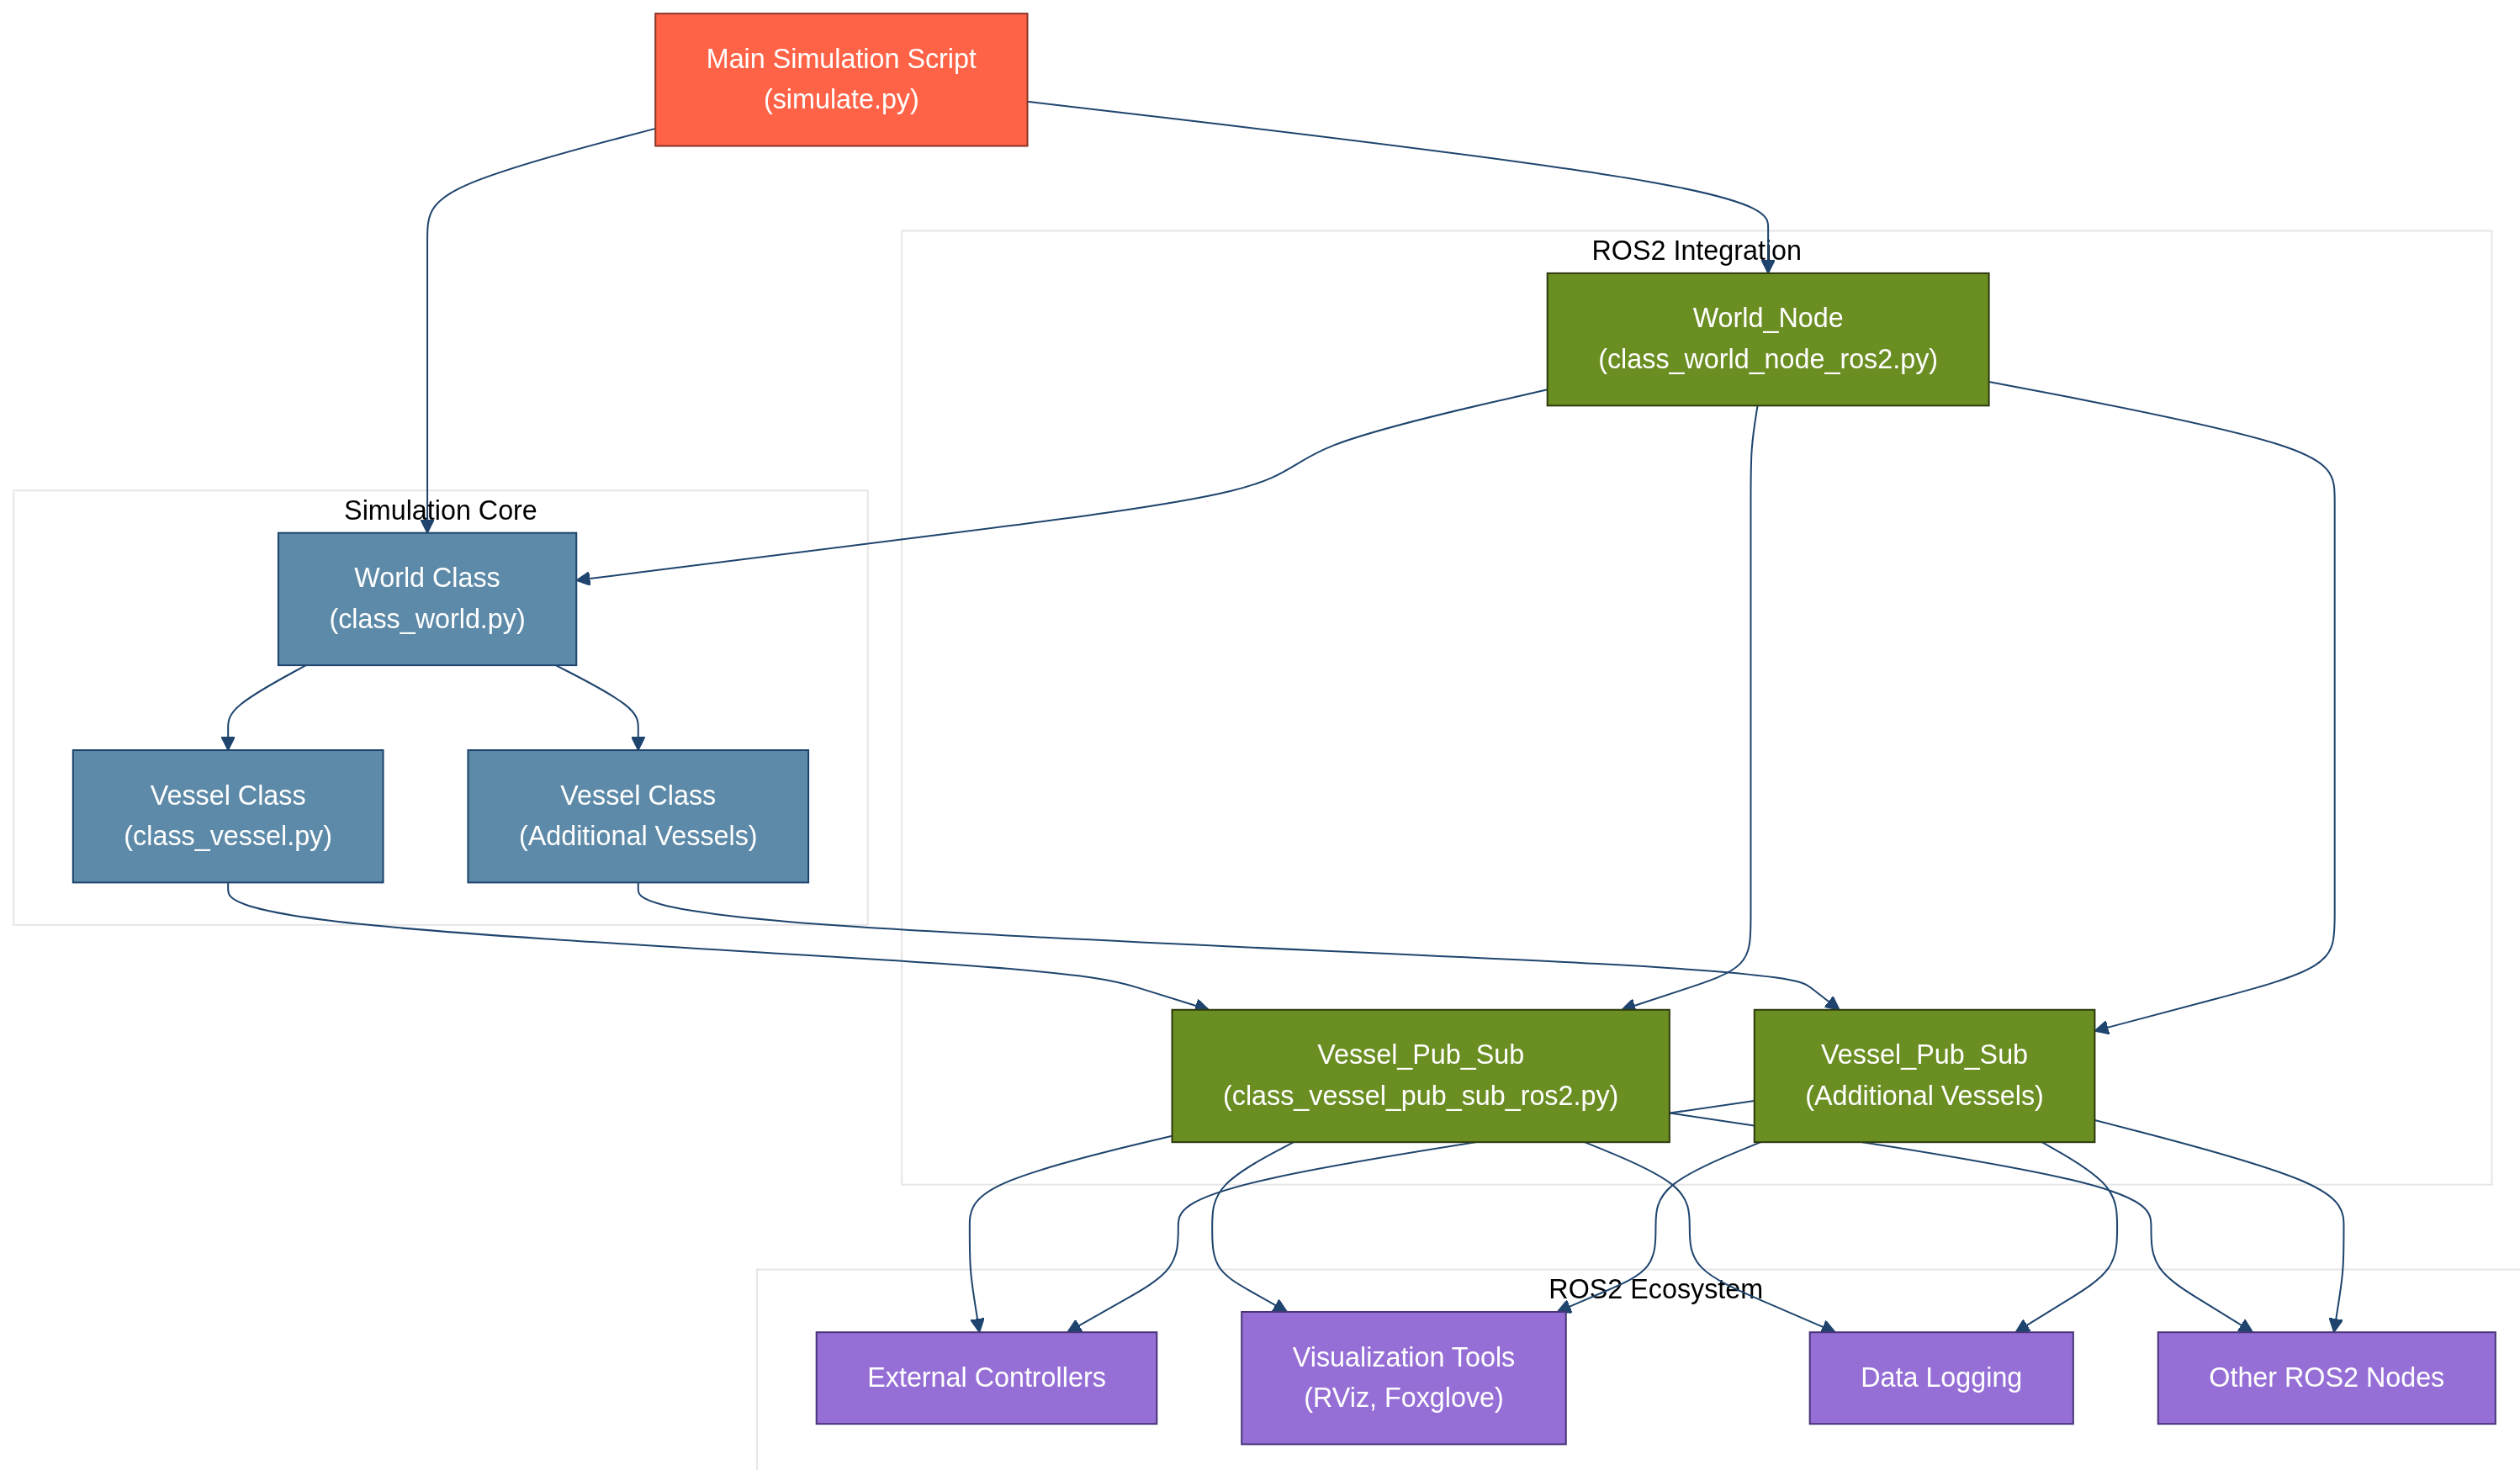
\includegraphics[width=15.76in,height=9.21in]{rawFiles/ROS2/ros2_files/figure-latex/mermaid-figure-1.png}

\textbf{Explanation of the Architecture Flow:}

\begin{itemize}
\tightlist
\item
  \textbf{Main Simulation Script (\texttt{simulate.py})}: Initiates the
  simulation by:

  \begin{itemize}
  \tightlist
  \item
    Calling \texttt{rclpy.init()} to initialize the ROS2 middleware
  \item
    Creating a \texttt{World} instance by calling
    \texttt{World(config\_file\_path)}
  \item
    Instantiating a \texttt{World\_Node} that wraps the simulation in
    ROS2
  \item
    Calling \texttt{world.start\_vessel\_ros\_nodes(world\_node)} to
    connect vessels to ROS2
  \end{itemize}
\item
  \textbf{World Class (\texttt{class\_world.py})}:

  \begin{itemize}
  \tightlist
  \item
    Maintains multiple vessel instances using
    \texttt{vessels\ =\ {[}{]}}
  \item
    Processes world input with
    \texttt{process\_world\_input(world\_file)}
  \item
    Creates vessels via
    \texttt{Vessel(vessel\_params,\ hydrodynamic\_data,\ vessel\_id)}
  \item
    Updates simulation state with \texttt{step()} method that calls
    \texttt{vessel.step()} for each vessel
  \end{itemize}
\item
  \textbf{World\_Node Class (\texttt{class\_world\_node\_ros2.py})}:

  \begin{itemize}
  \tightlist
  \item
    Inherits from ROS2 \texttt{Node} class
  \item
    Creates a timer with
    \texttt{create\_timer(1/self.rate,\ self.world.step)} to drive
    simulation
  \end{itemize}
\item
  \textbf{Vessel\_Pub\_Sub Class
  (\texttt{class\_vessel\_pub\_sub\_ros2.py})}:

  \begin{itemize}
  \tightlist
  \item
    Creates publishers, subscribers, and timers for each vessel
  \item
    Publishes vessel state and sensor data
  \item
    Handles actuator commands via subscribers
  \end{itemize}
\end{itemize}

\section*{Key Components}\label{key-components}
\addcontentsline{toc}{section}{Key Components}

\markright{Key Components}

\subsection*{\texorpdfstring{Main Simulation Script
(\texttt{simulate.py})}{Main Simulation Script (simulate.py)}}\label{main-simulation-script-simulate.py}
\addcontentsline{toc}{subsection}{Main Simulation Script
(\texttt{simulate.py})}

The entry point for running Panisim with ROS2 integration. This script:

\begin{enumerate}
\def\labelenumi{\arabic{enumi}.}
\tightlist
\item
  Initializes the ROS2 environment
\item
  Creates the World simulation instance
\item
  Sets up the World\_Node for ROS2 communication
\item
  Establishes connections between simulation and ROS2
\item
  Runs the ROS2 spin loop in a separate thread
\end{enumerate}

\begin{Shaded}
\begin{Highlighting}[]
\KeywordTok{def}\NormalTok{ main():}
    \CommentTok{\# Creates an object of class \textquotesingle{}World\textquotesingle{}}
\NormalTok{    rclpy.init()}
\NormalTok{    world }\OperatorTok{=}\NormalTok{ World(}\StringTok{\textquotesingle{}/workspaces/mavlab/inputs/simulation\_input.yml\textquotesingle{}}\NormalTok{)}
\NormalTok{    world\_node }\OperatorTok{=}\NormalTok{ World\_Node(world\_rate}\OperatorTok{=}\DecValTok{1}\OperatorTok{/}\NormalTok{world.dt)}
  
\NormalTok{    world.node }\OperatorTok{=}\NormalTok{ world\_node}
\NormalTok{    world.start\_vessel\_ros\_nodes(world\_node)}

    \CommentTok{\# Run ROS on a separate thread}
\NormalTok{    ros\_thread\_instance }\OperatorTok{=}\NormalTok{ threading.Thread(target}\OperatorTok{=}\NormalTok{ros\_thread, args}\OperatorTok{=}\NormalTok{(world\_node,))}
\NormalTok{    ros\_thread\_instance.start()}
    
    \CommentTok{\# Prints available ROS2 topics and usage information}
    \CommentTok{\# ...}
\end{Highlighting}
\end{Shaded}

The \texttt{ros\_thread} function is defined as:

\begin{Shaded}
\begin{Highlighting}[]
\KeywordTok{def}\NormalTok{ ros\_thread(node):}
\NormalTok{    rclpy.spin(node)}
\NormalTok{    rclpy.shutdown()}
\end{Highlighting}
\end{Shaded}

This function handles the ROS2 event loop, allowing callbacks to be
processed in the background while the main thread can perform other
tasks.

\subsection*{\texorpdfstring{World Class
(\texttt{class\_world.py})}{World Class (class\_world.py)}}\label{world-class-class_world.py}
\addcontentsline{toc}{subsection}{World Class
(\texttt{class\_world.py})}

The World class serves as the simulation environment container,
managing:

\begin{itemize}
\tightlist
\item
  Multiple vessel instances within a unified simulation
\item
  Initialization from configuration files
\item
  Simulation time stepping across all vessels
\item
  Global parameters like GPS datum and world boundaries
\end{itemize}

\begin{Shaded}
\begin{Highlighting}[]
\KeywordTok{class}\NormalTok{ World():}
\NormalTok{    terminate }\OperatorTok{=} \VariableTok{False}                   \CommentTok{\# Flag indicating simulation termination}
\NormalTok{    vessels }\OperatorTok{=}\NormalTok{ []                        }\CommentTok{\# List of Vessel objects}
\NormalTok{    nvessels }\OperatorTok{=} \DecValTok{0}                        \CommentTok{\# Number of vessels}
\NormalTok{    size }\OperatorTok{=}\NormalTok{ np.zeros(}\DecValTok{3}\NormalTok{)                  }\CommentTok{\# Size of the world (X{-}Y{-}Z)}
\NormalTok{    gps\_datum }\OperatorTok{=} \VariableTok{None}                    \CommentTok{\# GPS reference point}
\NormalTok{    node }\OperatorTok{=} \VariableTok{None}                         \CommentTok{\# ROS2 node reference}
\NormalTok{    dt }\OperatorTok{=} \FloatTok{0.01}                           \CommentTok{\# Simulation time step}

    \KeywordTok{def} \FunctionTok{\_\_init\_\_}\NormalTok{(}\VariableTok{self}\NormalTok{, world\_file}\OperatorTok{=}\VariableTok{None}\NormalTok{):}
        \CommentTok{"""Initialize the World object from configuration file"""}
        \ControlFlowTok{if}\NormalTok{ world\_file }\KeywordTok{is} \KeywordTok{not} \VariableTok{None}\NormalTok{:}
            \VariableTok{self}\NormalTok{.process\_world\_input(world\_file)}
    
    \KeywordTok{def}\NormalTok{ step(}\VariableTok{self}\NormalTok{):}
        \CommentTok{"""Advance the simulation by one time step"""}
        \ControlFlowTok{for}\NormalTok{ vessel }\KeywordTok{in} \VariableTok{self}\NormalTok{.vessels:}
\NormalTok{            vessel.step()}
\end{Highlighting}
\end{Shaded}

The \texttt{process\_world\_input} method reads the simulation
configuration from YAML files:

\begin{Shaded}
\begin{Highlighting}[]
\KeywordTok{def}\NormalTok{ process\_world\_input(}\VariableTok{self}\NormalTok{, world\_file}\OperatorTok{=}\VariableTok{None}\NormalTok{):}
    \ControlFlowTok{try}\NormalTok{:}
\NormalTok{        sim\_params, agents }\OperatorTok{=}\NormalTok{ read\_input(world\_file)}
        \VariableTok{self}\NormalTok{.size }\OperatorTok{=}\NormalTok{ np.array(sim\_params[}\StringTok{\textquotesingle{}world\_size\textquotesingle{}}\NormalTok{])}
        \VariableTok{self}\NormalTok{.nvessels }\OperatorTok{=}\NormalTok{ sim\_params[}\StringTok{\textquotesingle{}nagents\textquotesingle{}}\NormalTok{]}
        \VariableTok{self}\NormalTok{.gps\_datum }\OperatorTok{=}\NormalTok{ np.array(sim\_params[}\StringTok{\textquotesingle{}gps\_datum\textquotesingle{}}\NormalTok{])}
\NormalTok{        agent\_count }\OperatorTok{=} \DecValTok{0}
        \VariableTok{self}\NormalTok{.dt }\OperatorTok{=}\NormalTok{ sim\_params[}\StringTok{\textquotesingle{}time\_step\textquotesingle{}}\NormalTok{]}
        
        \ControlFlowTok{for}\NormalTok{ agent }\KeywordTok{in}\NormalTok{ agents[}\DecValTok{0}\NormalTok{:}\VariableTok{self}\NormalTok{.nvessels]:}
\NormalTok{            vessel\_config }\OperatorTok{=}\NormalTok{ agent[}\StringTok{\textquotesingle{}vessel\_config\textquotesingle{}}\NormalTok{]}
\NormalTok{            hydrodynamic\_data }\OperatorTok{=}\NormalTok{ agent[}\StringTok{\textquotesingle{}hydrodynamics\textquotesingle{}}\NormalTok{]}
            \VariableTok{self}\NormalTok{.vessels.append(Vessel(vessel\_params}\OperatorTok{=}\NormalTok{vessel\_config, }
\NormalTok{                                      hydrodynamic\_data}\OperatorTok{=}\NormalTok{hydrodynamic\_data, }
\NormalTok{                                      vessel\_id}\OperatorTok{=}\NormalTok{agent\_count))}
\NormalTok{            agent\_count }\OperatorTok{+=} \DecValTok{1}
    \ControlFlowTok{except}\NormalTok{ yaml.YAMLError }\ImportTok{as}\NormalTok{ exc:}
        \BuiltInTok{print}\NormalTok{(exc)}
\NormalTok{        exit()}
\end{Highlighting}
\end{Shaded}

The World class includes a method to start the ROS2 nodes for all
vessels:

\begin{Shaded}
\begin{Highlighting}[]
\KeywordTok{def}\NormalTok{ start\_vessel\_ros\_nodes(}\VariableTok{self}\NormalTok{, world\_node):}
    \CommentTok{"""Initialize ROS2 nodes for all vessels in the world"""}
    \ControlFlowTok{for}\NormalTok{ vessel }\KeywordTok{in} \VariableTok{self}\NormalTok{.vessels:}
\NormalTok{        vessel.vessel\_node }\OperatorTok{=}\NormalTok{ Vessel\_Pub\_Sub(vessel, world\_node)}
\end{Highlighting}
\end{Shaded}

\subsection*{\texorpdfstring{World\_Node Class
(\texttt{class\_world\_node\_ros2.py})}{World\_Node Class (class\_world\_node\_ros2.py)}}\label{world_node-class-class_world_node_ros2.py}
\addcontentsline{toc}{subsection}{World\_Node Class
(\texttt{class\_world\_node\_ros2.py})}

The World\_Node class is a ROS2 node wrapper for the World class:

\begin{Shaded}
\begin{Highlighting}[]
\KeywordTok{class}\NormalTok{ World\_Node(Node):}
\NormalTok{    rate }\OperatorTok{=} \VariableTok{None}
    \KeywordTok{def} \FunctionTok{\_\_init\_\_}\NormalTok{(}\VariableTok{self}\NormalTok{, world\_rate}\OperatorTok{=}\DecValTok{100}\NormalTok{, world\_file}\OperatorTok{=}\VariableTok{None}\NormalTok{):}
        \BuiltInTok{super}\NormalTok{().}\FunctionTok{\_\_init\_\_}\NormalTok{(}\StringTok{\textquotesingle{}world\textquotesingle{}}\NormalTok{)}
        \VariableTok{self}\NormalTok{.rate }\OperatorTok{=}\NormalTok{ world\_rate}
        \VariableTok{self}\NormalTok{.world }\OperatorTok{=}\NormalTok{ World(world\_file)}
        \VariableTok{self}\NormalTok{.create\_timer(}\DecValTok{1}\OperatorTok{/}\VariableTok{self}\NormalTok{.rate, callback}\OperatorTok{=}\VariableTok{self}\NormalTok{.world.step)}
\end{Highlighting}
\end{Shaded}

This class: - Inherits from the ROS2 Node class - Creates a timer that
triggers the simulation step function at a specified rate - Provides the
ROS2 context for the World class

The \texttt{create\_timer} method sets up a timer that calls the
\texttt{World.step()} method at regular intervals determined by
\texttt{world\_rate}. This is what drives the simulation forward in time
while maintaining synchronization with the ROS2 ecosystem.

\subsection*{\texorpdfstring{Vessel\_Pub\_Sub Class
(\texttt{class\_vessel\_pub\_sub\_ros2.py})}{Vessel\_Pub\_Sub Class (class\_vessel\_pub\_sub\_ros2.py)}}\label{vessel_pub_sub-class-class_vessel_pub_sub_ros2.py}
\addcontentsline{toc}{subsection}{Vessel\_Pub\_Sub Class
(\texttt{class\_vessel\_pub\_sub\_ros2.py})}

The Vessel\_Pub\_Sub class implements the ROS2 communication interface
for vessel objects:

\begin{Shaded}
\begin{Highlighting}[]
\KeywordTok{class}\NormalTok{ Vessel\_Pub\_Sub():}
    \KeywordTok{def} \FunctionTok{\_\_init\_\_}\NormalTok{(}\VariableTok{self}\NormalTok{, vessel, world\_node):}
        \CommentTok{"""Initialize the vessel interface"""}
        \VariableTok{self}\NormalTok{.world\_node }\OperatorTok{=}\NormalTok{ world\_node}
        \VariableTok{self}\NormalTok{.vessel }\OperatorTok{=}\NormalTok{ vessel}
        \VariableTok{self}\NormalTok{.vessel\_id }\OperatorTok{=}\NormalTok{ vessel.vessel\_id}
        \VariableTok{self}\NormalTok{.vessel\_name }\OperatorTok{=}\NormalTok{ vessel.vessel\_name}
        \VariableTok{self}\NormalTok{.topic\_prefix }\OperatorTok{=} \SpecialStringTok{f\textquotesingle{}}\SpecialCharTok{\{}\VariableTok{self}\SpecialCharTok{.}\NormalTok{vessel\_name}\SpecialCharTok{\}}\SpecialStringTok{\_}\SpecialCharTok{\{}\VariableTok{self}\SpecialCharTok{.}\NormalTok{vessel\_id}\SpecialCharTok{:02d\}}\SpecialStringTok{\textquotesingle{}}
        
        \CommentTok{\# Initialize publishers, subscribers, and timers}
        \CommentTok{\# ...}
\end{Highlighting}
\end{Shaded}

This class:

\begin{itemize}
\tightlist
\item
  Creates and manages ROS2 publishers for vessel state and sensor data
\item
  Sets up subscribers for actuator commands
\item
  Handles message conversion between simulator data and ROS2 messages
\item
  Manages sensor data publication at appropriate rates
\end{itemize}

Key initialization methods include:

\begin{itemize}
\tightlist
\item
  Setting up control surface and thruster mappings
\item
  Creating sensor objects and their publishers
\item
  Initializing odometry and vessel state publishers
\item
  Creating actuator command subscribers
\end{itemize}

\section*{Message Flow}\label{message-flow}
\addcontentsline{toc}{section}{Message Flow}

\markright{Message Flow}

The communication between simulation components and the ROS2 ecosystem
follows this message flow:

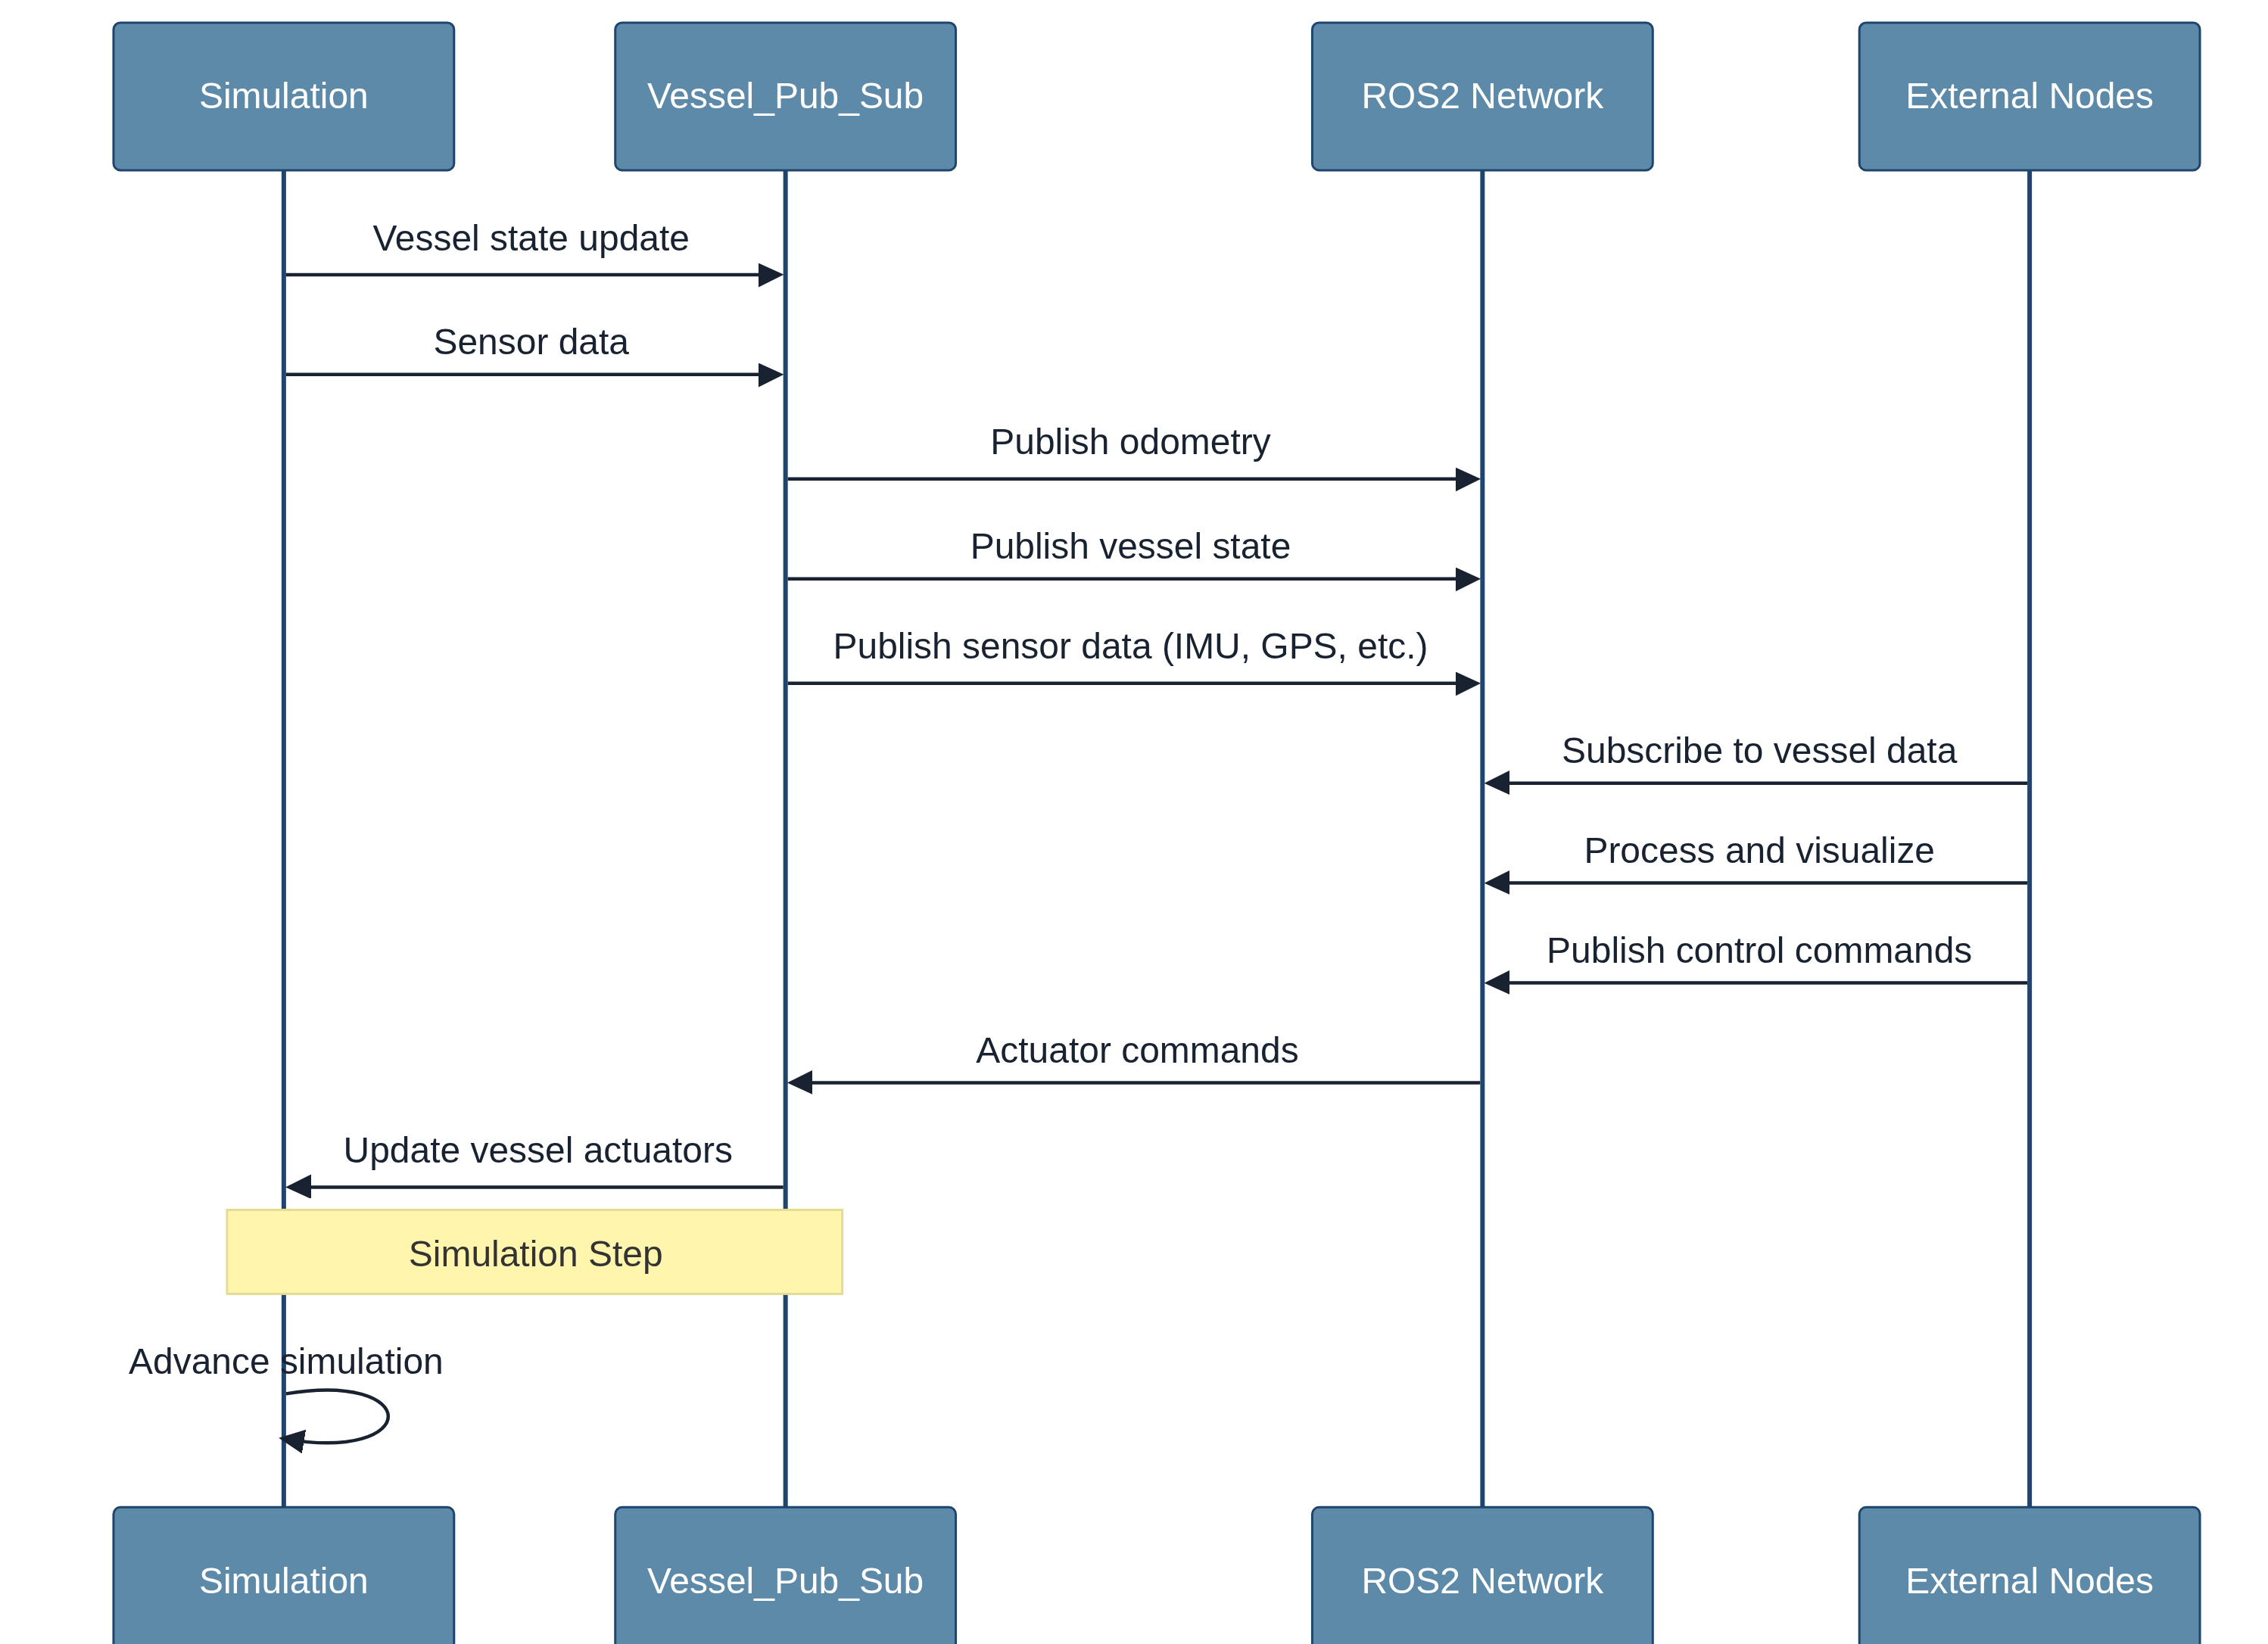
\includegraphics[width=10.61in,height=7.71in]{rawFiles/ROS2/ros2_files/figure-latex/mermaid-figure-5.png}

\textbf{Detailed Function Call Sequence:}

\begin{enumerate}
\def\labelenumi{\arabic{enumi}.}
\tightlist
\item
  \textbf{Vessel State Update}:

  \begin{itemize}
  \tightlist
  \item
    \texttt{vessel.step()} in \texttt{World.step()} updates the vessel
    state
  \item
    This updates \texttt{vessel.current\_state}, which is accessed by
    publishers
  \end{itemize}
\item
  \textbf{Sensor Data Generation}:

  \begin{itemize}
  \tightlist
  \item
    Sensor objects call \texttt{get\_measurement()} to generate
    simulated sensor readings based on vessel state
  \end{itemize}
\item
  \textbf{Publishing Data to ROS2}:

  \begin{itemize}
  \tightlist
  \item
    \texttt{publish\_odometry()} is called by a timer to publish vessel
    position and orientation
  \item
    \texttt{publish\_vessel\_state()} is called by a timer to publish
    complete state vector
  \item
    \texttt{\_publish\_sensor()} is called by sensor-specific timers to
    publish sensor data
  \end{itemize}
\item
  \textbf{External Nodes Subscribing}:

  \begin{itemize}
  \tightlist
  \item
    External ROS2 nodes subscribe to topics using
    \texttt{ros2\ topic\ echo} or programmatically
  \end{itemize}
\item
  \textbf{Control Commands}:

  \begin{itemize}
  \tightlist
  \item
    External nodes publish to
    \texttt{/\textless{}vessel\_name\textgreater{}\_\textless{}id\textgreater{}/actuator\_cmd}
  \item
    \texttt{actuator\_callback(msg)} processes these commands
  \end{itemize}
\item
  \textbf{Updating Actuator States}:

  \begin{itemize}
  \tightlist
  \item
    \texttt{vessel.delta\_c} (control surfaces) and \texttt{vessel.n\_c}
    (thrusters) are updated
  \item
    These affect the vessel dynamics in the next simulation step
  \end{itemize}
\item
  \textbf{Simulation Step}:

  \begin{itemize}
  \tightlist
  \item
    The timer in \texttt{World\_Node} triggers \texttt{world.step()}
  \item
    This advances all vessels' states using their dynamics models
  \end{itemize}
\end{enumerate}

\section*{Topics and Messages}\label{topics-and-messages}
\addcontentsline{toc}{section}{Topics and Messages}

\markright{Topics and Messages}

Each vessel in the simulation publishes data on several ROS2 topics:

\subsection*{Standard Topics}\label{standard-topics}
\addcontentsline{toc}{subsection}{Standard Topics}

\begin{longtable}[]{@{}
  >{\raggedright\arraybackslash}p{(\linewidth - 4\tabcolsep) * \real{0.2059}}
  >{\raggedright\arraybackslash}p{(\linewidth - 4\tabcolsep) * \real{0.4118}}
  >{\raggedright\arraybackslash}p{(\linewidth - 4\tabcolsep) * \real{0.3824}}@{}}
\toprule\noalign{}
\begin{minipage}[b]{\linewidth}\raggedright
Topic
\end{minipage} & \begin{minipage}[b]{\linewidth}\raggedright
Message Type
\end{minipage} & \begin{minipage}[b]{\linewidth}\raggedright
Description
\end{minipage} \\
\midrule\noalign{}
\endhead
\bottomrule\noalign{}
\endlastfoot
\texttt{/\textless{}vessel\_name\textgreater{}\_\textless{}id\textgreater{}/odometry\_sim}
& \texttt{nav\_msgs/Odometry} & Vessel position, orientation, and
velocities \\
\texttt{/\textless{}vessel\_name\textgreater{}\_\textless{}id\textgreater{}/vessel\_state}
& \texttt{std\_msgs/Float64MultiArray} & Complete vessel state including
actuators \\
\texttt{/\textless{}vessel\_name\textgreater{}\_\textless{}id\textgreater{}/actuator\_cmd}
& \texttt{interfaces/Actuator} & Commands for control surfaces and
thrusters \\
\end{longtable}

\subsection*{Sensor Topics}\label{sensor-topics}
\addcontentsline{toc}{subsection}{Sensor Topics}

Each sensor configured for a vessel publishes on its own topic:

\begin{longtable}[]{@{}
  >{\raggedright\arraybackslash}p{(\linewidth - 4\tabcolsep) * \real{0.2759}}
  >{\raggedright\arraybackslash}p{(\linewidth - 4\tabcolsep) * \real{0.2414}}
  >{\raggedright\arraybackslash}p{(\linewidth - 4\tabcolsep) * \real{0.4828}}@{}}
\toprule\noalign{}
\begin{minipage}[b]{\linewidth}\raggedright
Sensor
\end{minipage} & \begin{minipage}[b]{\linewidth}\raggedright
Topic
\end{minipage} & \begin{minipage}[b]{\linewidth}\raggedright
Message Type
\end{minipage} \\
\midrule\noalign{}
\endhead
\bottomrule\noalign{}
\endlastfoot
IMU &
\texttt{/\textless{}vessel\_name\textgreater{}\_\textless{}id\textgreater{}/imu}
& \texttt{sensor\_msgs/Imu} \\
GPS &
\texttt{/\textless{}vessel\_name\textgreater{}\_\textless{}id\textgreater{}/gps}
& \texttt{sensor\_msgs/NavSatFix} \\
DVL &
\texttt{/\textless{}vessel\_name\textgreater{}\_\textless{}id\textgreater{}/dvl}
& \texttt{interfaces/DVL} \\
UWB &
\texttt{/\textless{}vessel\_name\textgreater{}\_\textless{}id\textgreater{}/uwb}
& \texttt{geometry\_msgs/PoseWithCovarianceStamped} \\
\end{longtable}

\section*{Sensor Integration}\label{sensor-integration}
\addcontentsline{toc}{section}{Sensor Integration}

\markright{Sensor Integration}

Sensors are created and managed through the Vessel\_Pub\_Sub class:

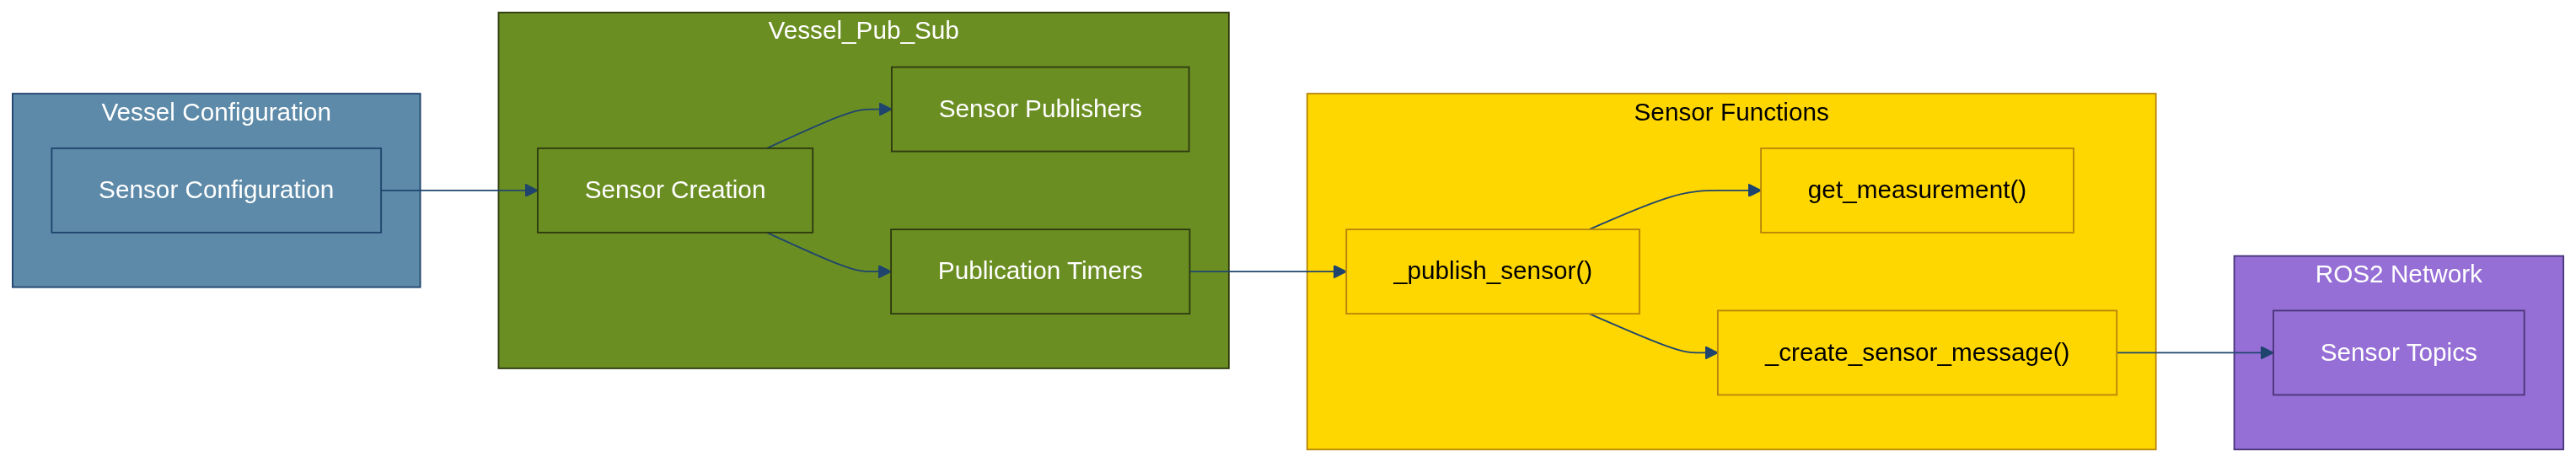
\includegraphics[width=17.13in,height=3.08in]{rawFiles/ROS2/ros2_files/figure-latex/mermaid-figure-4.png}

\textbf{Detailed Function Calls in Sensor Integration:}

\begin{enumerate}
\def\labelenumi{\arabic{enumi}.}
\tightlist
\item
  \textbf{SensorConfig to SensorCreation}:

  \begin{itemize}
  \tightlist
  \item
    During \texttt{Vessel\_Pub\_Sub} initialization, it reads sensor
    configurations from
    \texttt{vessel.vessel\_config{[}\textquotesingle{}sensors\textquotesingle{}{]}}
  \item
    For each sensor configuration, it calls
    \texttt{create\_sensor(sensor\_config,\ vessel\_id,\ topic\_prefix,\ self)}
  \end{itemize}
\item
  \textbf{SensorCreation to Publishers and Timers}:

  \begin{itemize}
  \item
    After creating a sensor object, \texttt{Vessel\_Pub\_Sub} creates a
    publisher using:

\begin{Shaded}
\begin{Highlighting}[]
\VariableTok{self}\NormalTok{.world\_node.create\_publisher(}\VariableTok{self}\NormalTok{.\_get\_msg\_type(sensor.sensor\_type), sensor\_topic, }\DecValTok{10}\NormalTok{)}
\end{Highlighting}
\end{Shaded}
  \item
    It also creates a timer for each sensor:

\begin{Shaded}
\begin{Highlighting}[]
\VariableTok{self}\NormalTok{.world\_node.create\_timer(}\DecValTok{1}\OperatorTok{/}\NormalTok{sensor.rate, }\KeywordTok{lambda}\NormalTok{ s}\OperatorTok{=}\NormalTok{sensor: }\VariableTok{self}\NormalTok{.\_publish\_sensor(s))}
\end{Highlighting}
\end{Shaded}
  \end{itemize}
\item
  \textbf{Timer to PublishSensor}:

  \begin{itemize}
  \tightlist
  \item
    Each timer periodically calls \texttt{\_publish\_sensor(sensor)} at
    the sensor's configured rate
  \end{itemize}
\item
  \textbf{PublishSensor to GetMeasurement}:

  \begin{itemize}
  \tightlist
  \item
    The \texttt{\_publish\_sensor} method calls
    \texttt{sensor.get\_measurement()} to obtain the latest sensor
    reading
  \item
    Each sensor type has its own implementation of
    \texttt{get\_measurement()}
  \end{itemize}
\item
  \textbf{PublishSensor to CreateMessage}:

  \begin{itemize}
  \tightlist
  \item
    After getting the measurement, \texttt{\_publish\_sensor} calls
    \texttt{\_create\_sensor\_message(sensor\_type,\ measurement)}
  \item
    This converts the measurement to the appropriate ROS2 message type
  \end{itemize}
\item
  \textbf{CreateMessage to Topics}:

  \begin{itemize}
  \item
    Finally, the message is published to the ROS2 network:

\begin{Shaded}
\begin{Highlighting}[]
\NormalTok{s[}\StringTok{\textquotesingle{}pub\textquotesingle{}}\NormalTok{].publish(msg)}
\end{Highlighting}
\end{Shaded}
  \end{itemize}
\end{enumerate}

The process for sensor integration:

\begin{enumerate}
\def\labelenumi{\arabic{enumi}.}
\tightlist
\item
  Sensor configurations are defined in the vessel parameters (input
  files \texttt{sensors.yml})
\item
  The Vessel\_Pub\_Sub class creates sensor objects using the
  \texttt{create\_sensor} factory function
\item
  For each sensor, a publisher and timer are created
\item
  The timer periodically calls the sensor's \texttt{get\_measurement()}
  method
\item
  Measurements are converted to ROS2 messages and published
\end{enumerate}

Key methods in the sensor integration:

\begin{Shaded}
\begin{Highlighting}[]
\KeywordTok{def}\NormalTok{ \_publish\_sensor(}\VariableTok{self}\NormalTok{, sensor):}
    \CommentTok{"""Publish sensor data."""}
\NormalTok{    measurement }\OperatorTok{=}\NormalTok{ sensor.get\_measurement()}
\NormalTok{    msg }\OperatorTok{=} \VariableTok{self}\NormalTok{.\_create\_sensor\_message(sensor.sensor\_type, measurement)}
    
    \CommentTok{\# Find the publisher for this sensor}
    \ControlFlowTok{for}\NormalTok{ s }\KeywordTok{in} \VariableTok{self}\NormalTok{.sensors:}
        \ControlFlowTok{if}\NormalTok{ s[}\StringTok{\textquotesingle{}sensor\textquotesingle{}}\NormalTok{] }\OperatorTok{==}\NormalTok{ sensor:}
\NormalTok{            s[}\StringTok{\textquotesingle{}pub\textquotesingle{}}\NormalTok{].publish(msg)}
            \ControlFlowTok{break}
\end{Highlighting}
\end{Shaded}

\begin{Shaded}
\begin{Highlighting}[]
\KeywordTok{def}\NormalTok{ \_create\_sensor\_message(}\VariableTok{self}\NormalTok{, sensor\_type, measurement):}
    \CommentTok{"""Create a ROS message for sensor data."""}
\NormalTok{    current\_time }\OperatorTok{=} \VariableTok{self}\NormalTok{.world\_node.get\_clock().now().to\_msg()}
    
    \CommentTok{\# Create appropriate message based on sensor type}
    \ControlFlowTok{if}\NormalTok{ sensor\_type }\OperatorTok{==} \StringTok{\textquotesingle{}IMU\textquotesingle{}}\NormalTok{:}
\NormalTok{        msg }\OperatorTok{=}\NormalTok{ Imu()}
        \CommentTok{\# Fill message fields}
    \ControlFlowTok{elif}\NormalTok{ sensor\_type }\OperatorTok{==} \StringTok{\textquotesingle{}GPS\textquotesingle{}}\NormalTok{:}
\NormalTok{        msg }\OperatorTok{=}\NormalTok{ NavSatFix()}
        \CommentTok{\# Fill message fields}
    \CommentTok{\# ... other sensor types}
    
    \ControlFlowTok{return}\NormalTok{ msg}
\end{Highlighting}
\end{Shaded}

\section*{Actuator Control}\label{actuator-control}
\addcontentsline{toc}{section}{Actuator Control}

\markright{Actuator Control}

Vessels can be controlled through ROS2 by sending actuator commands:

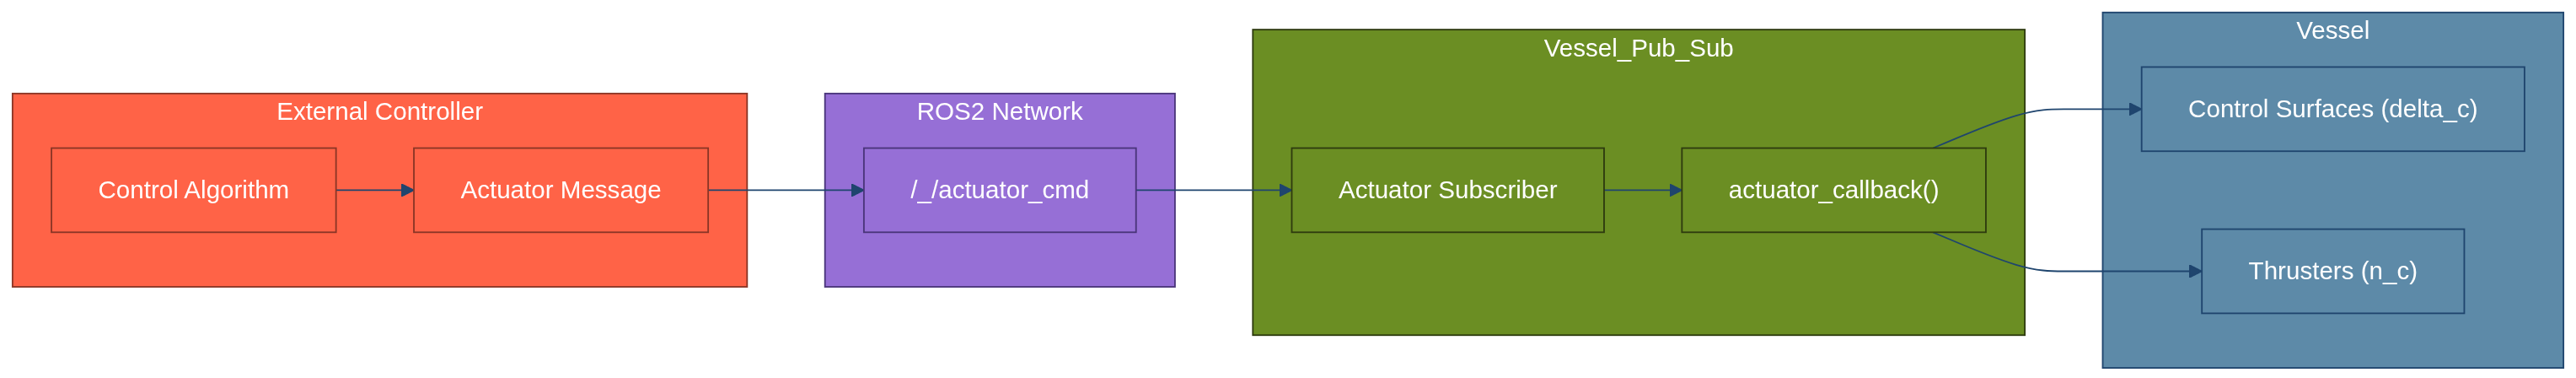
\includegraphics[width=17.23in,height=2.54in]{rawFiles/ROS2/ros2_files/figure-latex/mermaid-figure-3.png}

\textbf{Detailed Function Calls in Actuator Control:}

\begin{enumerate}
\def\labelenumi{\arabic{enumi}.}
\tightlist
\item
  \textbf{ControlAlgorithm to ActuatorMsg}:

  \begin{itemize}
  \tightlist
  \item
    External control algorithms compute desired actuator values
  \item
    They create an \texttt{Actuator} message with the desired values
  \end{itemize}
\item
  \textbf{ActuatorMsg to ActuatorTopic}:

  \begin{itemize}
  \tightlist
  \item
    The controller publishes the message to the actuator command topic
  \item
    This is done using ROS2's \texttt{publisher.publish(msg)} mechanism
  \end{itemize}
\item
  \textbf{ActuatorTopic to Subscriber}:

  \begin{itemize}
  \item
    The subscriber in \texttt{Vessel\_Pub\_Sub} receives the message
  \item
    This was set up during initialization with:

\begin{Shaded}
\begin{Highlighting}[]
\VariableTok{self}\NormalTok{.actuator\_sub }\OperatorTok{=} \VariableTok{self}\NormalTok{.world\_node.create\_subscription(}
\NormalTok{    Actuator, }
    \SpecialStringTok{f\textquotesingle{}}\SpecialCharTok{\{}\VariableTok{self}\SpecialCharTok{.}\NormalTok{topic\_prefix}\SpecialCharTok{\}}\SpecialStringTok{/actuator\_cmd\textquotesingle{}}\NormalTok{, }
    \VariableTok{self}\NormalTok{.actuator\_callback, }
    \DecValTok{1}
\NormalTok{)}
\end{Highlighting}
\end{Shaded}
  \end{itemize}
\item
  \textbf{Subscriber to Callback}:

  \begin{itemize}
  \tightlist
  \item
    The subscriber triggers \texttt{actuator\_callback(msg)} in
    \texttt{Vessel\_Pub\_Sub}
  \end{itemize}
\item
  \textbf{Callback to ControlSurfaces and Thrusters}:

  \begin{itemize}
  \item
    The callback parses the message and updates vessel control values:

\begin{Shaded}
\begin{Highlighting}[]
\CommentTok{\# For control surfaces}
\VariableTok{self}\NormalTok{.vessel.delta\_c[idx] }\OperatorTok{=}\NormalTok{ value }\OperatorTok{*}\NormalTok{ np.pi }\OperatorTok{/} \FloatTok{180.0}

\CommentTok{\# For thrusters}
\VariableTok{self}\NormalTok{.vessel.n\_c[idx] }\OperatorTok{=}\NormalTok{ value}
\end{Highlighting}
\end{Shaded}
  \end{itemize}
\end{enumerate}

\subsection*{\texorpdfstring{Actuator Message Structure
(\texttt{Actuator.msg})}{Actuator Message Structure (Actuator.msg)}}\label{actuator-message-structure-actuator.msg}
\addcontentsline{toc}{subsection}{Actuator Message Structure
(\texttt{Actuator.msg})}

The \texttt{Actuator.msg} is a custom message type used for controlling
vessel actuators. Its structure is:

\begin{verbatim}
std_msgs/Header header       # Standard header with timestamp
string[] actuator_names      # Array of actuator identifiers
float64[] actuator_values    # Array of corresponding values
\end{verbatim}

The actuator names use a prefixing convention: - \texttt{cs\_N} for
control surfaces (e.g., \texttt{cs\_1} for the first control surface) -
\texttt{th\_N} for thrusters (e.g., \texttt{th\_1} for the first
thruster)

Values for control surfaces are specified in \textbf{degrees} (converted
to radians internally) and values for thrusters are in \textbf{RPM}
(Revolutions Per Minute).

Example usage in \texttt{class\_vessel\_pub\_sub\_ros2.py}:

\begin{Shaded}
\begin{Highlighting}[]
\KeywordTok{def}\NormalTok{ actuator\_callback(}\VariableTok{self}\NormalTok{, msg):}
    \CommentTok{"""Handle actuator command messages."""}
    \ControlFlowTok{if} \BuiltInTok{len}\NormalTok{(msg.actuator\_names) }\OperatorTok{!=} \BuiltInTok{len}\NormalTok{(msg.actuator\_values):}
        \VariableTok{self}\NormalTok{.world\_node.get\_logger().warn(}\StringTok{\textquotesingle{}Mismatch between actuator IDs and values length\textquotesingle{}}\NormalTok{)}
        \ControlFlowTok{return}
        
    \ControlFlowTok{for}\NormalTok{ actuator\_id, value }\KeywordTok{in} \BuiltInTok{zip}\NormalTok{(msg.actuator\_names, msg.actuator\_values):}
        \ControlFlowTok{try}\NormalTok{:}
            \ControlFlowTok{if}\NormalTok{ actuator\_id.startswith(}\StringTok{\textquotesingle{}cs\_\textquotesingle{}}\NormalTok{):}
                \CommentTok{\# Handle control surface (convert degrees to radians)}
                \ControlFlowTok{if}\NormalTok{ actuator\_id }\KeywordTok{in} \VariableTok{self}\NormalTok{.control\_surface\_ids:}
\NormalTok{                    idx }\OperatorTok{=} \VariableTok{self}\NormalTok{.control\_surface\_ids[actuator\_id]}
                    \VariableTok{self}\NormalTok{.vessel.delta\_c[idx] }\OperatorTok{=}\NormalTok{ value }\OperatorTok{*}\NormalTok{ np.pi }\OperatorTok{/} \FloatTok{180.0}
                \ControlFlowTok{else}\NormalTok{:}
                    \VariableTok{self}\NormalTok{.world\_node.get\_logger().warn(}\SpecialStringTok{f\textquotesingle{}Unknown control surface ID: }\SpecialCharTok{\{}\NormalTok{actuator\_id}\SpecialCharTok{\}}\SpecialStringTok{\textquotesingle{}}\NormalTok{)}
                    
            \ControlFlowTok{elif}\NormalTok{ actuator\_id.startswith(}\StringTok{\textquotesingle{}th\_\textquotesingle{}}\NormalTok{):}
                \CommentTok{\# Handle thruster (RPM value)}
                \ControlFlowTok{if}\NormalTok{ actuator\_id }\KeywordTok{in} \VariableTok{self}\NormalTok{.thruster\_ids:}
\NormalTok{                    idx }\OperatorTok{=} \VariableTok{self}\NormalTok{.thruster\_ids[actuator\_id]}
                    \VariableTok{self}\NormalTok{.vessel.n\_c[idx] }\OperatorTok{=}\NormalTok{ value}
                \ControlFlowTok{else}\NormalTok{:}
                    \VariableTok{self}\NormalTok{.world\_node.get\_logger().warn(}\SpecialStringTok{f\textquotesingle{}Unknown thruster ID: }\SpecialCharTok{\{}\NormalTok{actuator\_id}\SpecialCharTok{\}}\SpecialStringTok{\textquotesingle{}}\NormalTok{)}
                    
            \ControlFlowTok{else}\NormalTok{:}
                \VariableTok{self}\NormalTok{.world\_node.get\_logger().warn(}\SpecialStringTok{f\textquotesingle{}Invalid actuator ID format: }\SpecialCharTok{\{}\NormalTok{actuator\_id}\SpecialCharTok{\}}\SpecialStringTok{. Must start with cs\_ or th\_\textquotesingle{}}\NormalTok{)}
        \ControlFlowTok{except}\NormalTok{ (}\PreprocessorTok{ValueError}\NormalTok{, }\PreprocessorTok{IndexError}\NormalTok{):}
            \VariableTok{self}\NormalTok{.world\_node.get\_logger().warn(}\SpecialStringTok{f\textquotesingle{}Unknown actuator ID: }\SpecialCharTok{\{}\NormalTok{actuator\_id}\SpecialCharTok{\}}\SpecialStringTok{\textquotesingle{}}\NormalTok{)}
\end{Highlighting}
\end{Shaded}

During initialization, \texttt{Vessel\_Pub\_Sub} builds mappings between
actuator IDs (as defined in \texttt{control\_surfaces.yml} and
\texttt{thrusters.yml}) and their indices:

\begin{Shaded}
\begin{Highlighting}[]
\CommentTok{\# Store actuator IDs with type prefixes}
\VariableTok{self}\NormalTok{.control\_surface\_ids }\OperatorTok{=}\NormalTok{ \{\}  }\CommentTok{\# Maps \textquotesingle{}cs\_id\textquotesingle{} to index}
\VariableTok{self}\NormalTok{.thruster\_ids }\OperatorTok{=}\NormalTok{ \{\}        }\CommentTok{\# Maps \textquotesingle{}th\_id\textquotesingle{} to index}
    
\ControlFlowTok{for}\NormalTok{ idx, cs }\KeywordTok{in} \BuiltInTok{enumerate}\NormalTok{(}\VariableTok{self}\NormalTok{.control\_surfaces):}
\NormalTok{    cs\_id }\OperatorTok{=}\NormalTok{ cs.get(}\StringTok{\textquotesingle{}control\_surface\_id\textquotesingle{}}\NormalTok{, idx}\OperatorTok{+}\DecValTok{1}\NormalTok{)}
    \VariableTok{self}\NormalTok{.control\_surface\_ids[}\SpecialStringTok{f\textquotesingle{}cs\_}\SpecialCharTok{\{}\NormalTok{cs\_id}\SpecialCharTok{\}}\SpecialStringTok{\textquotesingle{}}\NormalTok{] }\OperatorTok{=}\NormalTok{ idx}

\ControlFlowTok{for}\NormalTok{ idx, th }\KeywordTok{in} \BuiltInTok{enumerate}\NormalTok{(}\VariableTok{self}\NormalTok{.thrusters):}
\NormalTok{    th\_id }\OperatorTok{=}\NormalTok{ th.get(}\StringTok{\textquotesingle{}thruster\_id\textquotesingle{}}\NormalTok{, idx}\OperatorTok{+}\DecValTok{1}\NormalTok{)}
    \VariableTok{self}\NormalTok{.thruster\_ids[}\SpecialStringTok{f\textquotesingle{}th\_}\SpecialCharTok{\{}\NormalTok{th\_id}\SpecialCharTok{\}}\SpecialStringTok{\textquotesingle{}}\NormalTok{] }\OperatorTok{=}\NormalTok{ idx}
\end{Highlighting}
\end{Shaded}

These mappings ensure that actuator commands are properly routed to the
correct control surfaces and thrusters in the vessel's internal state.

\section*{World and Vessel
Population}\label{world-and-vessel-population}
\addcontentsline{toc}{section}{World and Vessel Population}

\markright{World and Vessel Population}

The process of populating the world with vessels follows these steps:

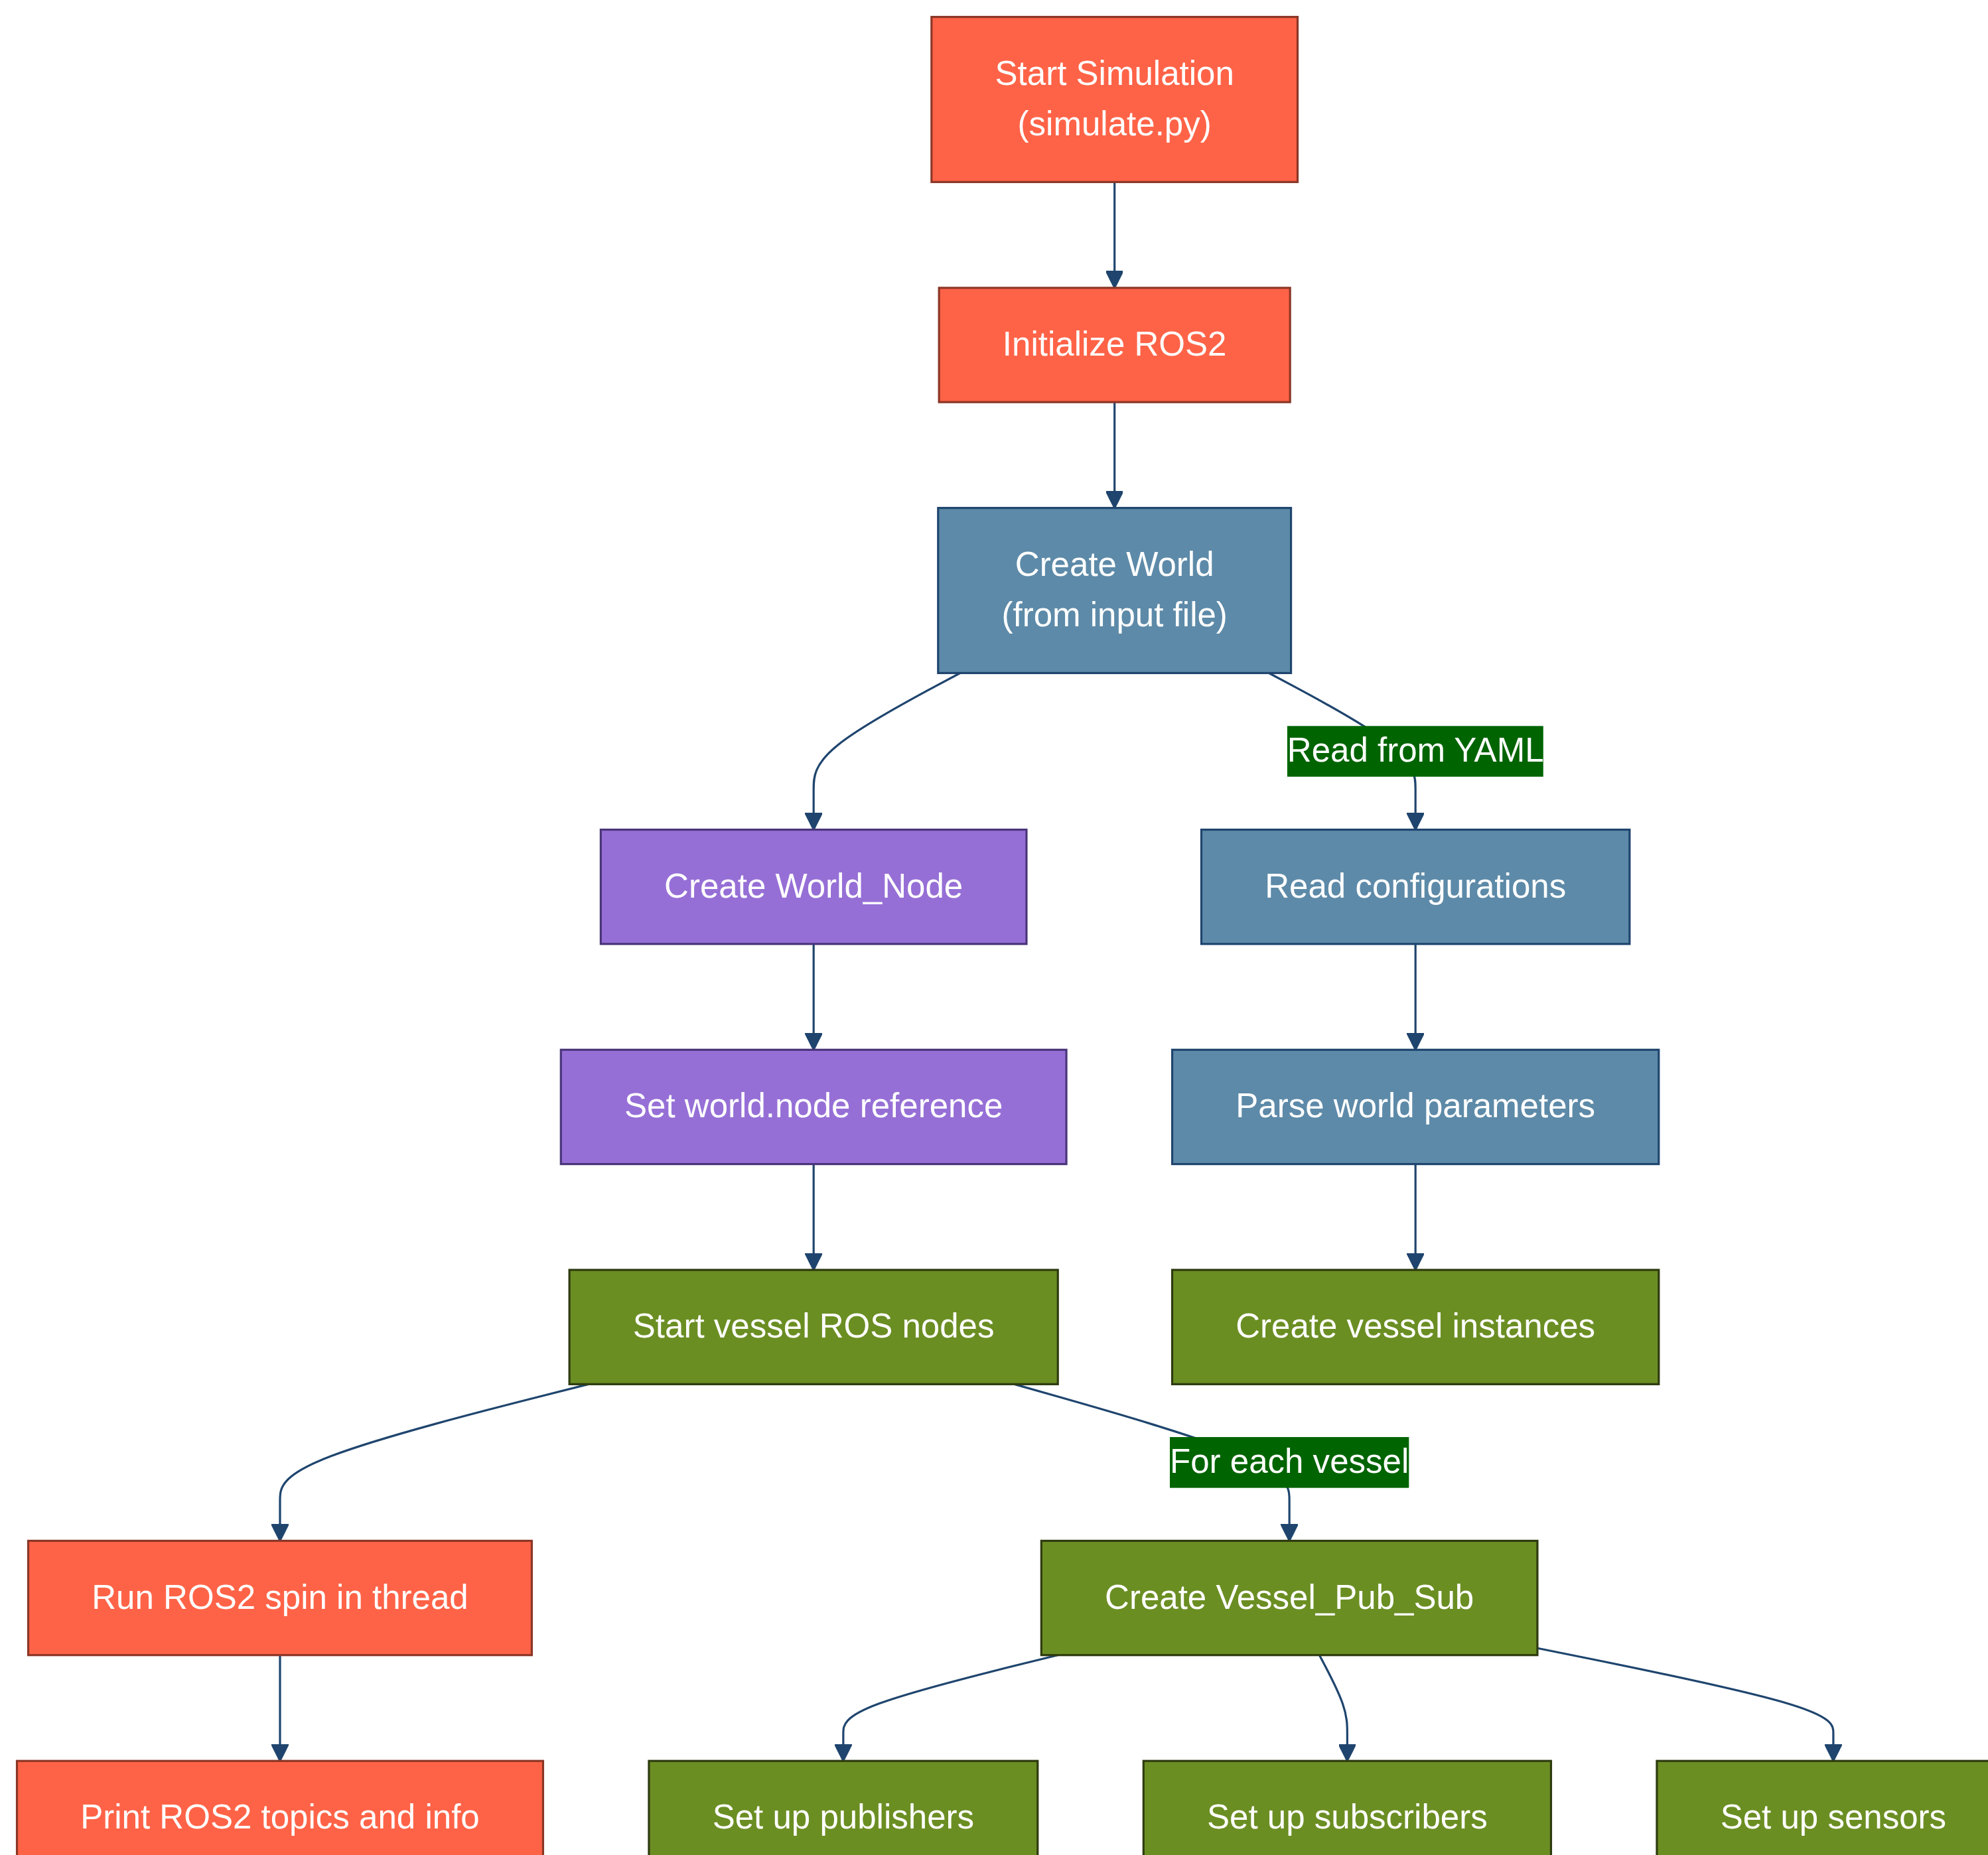
\includegraphics[width=9.97in,height=9.31in]{rawFiles/ROS2/ros2_files/figure-latex/mermaid-figure-2.png}

\textbf{Detailed Function Calls in World and Vessel Population:}

\begin{enumerate}
\def\labelenumi{\arabic{enumi}.}
\tightlist
\item
  \textbf{Start to Init}:

  \begin{itemize}
  \tightlist
  \item
    \texttt{simulate.py} starts and calls \texttt{rclpy.init()} to
    initialize the ROS2 middleware
  \item
    This initializes the ROS2 context for the application
  \end{itemize}
\item
  \textbf{Init to CreateWorld}:

  \begin{itemize}
  \tightlist
  \item
    \texttt{World(\textquotesingle{}/workspaces/mavlab/inputs/simulation\_input.yml\textquotesingle{})}
    is called
  \item
    This creates the World instance and loads configuration
  \end{itemize}
\item
  \textbf{CreateWorld to ReadConfig}:

  \begin{itemize}
  \tightlist
  \item
    \texttt{World.\_\_init\_\_} calls
    \texttt{self.process\_world\_input(world\_file)}
  \item
    \texttt{process\_world\_input} calls
    \texttt{read\_input(world\_file)} to parse YAML
  \end{itemize}
\item
  \textbf{ReadConfig to ParseWorld}:

  \begin{itemize}
  \tightlist
  \item
    \texttt{process\_world\_input} extracts world parameters like:

    \begin{itemize}
    \tightlist
    \item
      \texttt{self.size\ =\ np.array(sim\_params{[}\textquotesingle{}world\_size\textquotesingle{}{]})}
    \item
      \texttt{self.nvessels\ =\ sim\_params{[}\textquotesingle{}nagents\textquotesingle{}{]}}
    \item
      \texttt{self.gps\_datum\ =\ np.array(sim\_params{[}\textquotesingle{}gps\_datum\textquotesingle{}{]})}
    \end{itemize}
  \end{itemize}
\item
  \textbf{ParseWorld to CreateVessels}:

  \begin{itemize}
  \item
    \texttt{process\_world\_input} creates vessel instances:

\begin{Shaded}
\begin{Highlighting}[]
\VariableTok{self}\NormalTok{.vessels.append(Vessel(vessel\_params}\OperatorTok{=}\NormalTok{vessel\_config,}
\NormalTok{                          hydrodynamic\_data}\OperatorTok{=}\NormalTok{hydrodynamic\_data,}
\NormalTok{                          vessel\_id}\OperatorTok{=}\NormalTok{agent\_count))}
\end{Highlighting}
\end{Shaded}
  \end{itemize}
\item
  \textbf{CreateWorld to CreateNode}:

  \begin{itemize}
  \tightlist
  \item
    \texttt{World\_Node(world\_rate=1/world.dt)} is called
  \item
    This creates a ROS2 node wrapper for the World
  \end{itemize}
\item
  \textbf{SetNode to StartVessels}:

  \begin{itemize}
  \tightlist
  \item
    \texttt{world.start\_vessel\_ros\_nodes(world\_node)} is called
  \item
    This iterates through vessels and creates ROS2 interfaces
  \end{itemize}
\item
  \textbf{StartVessels to CreateVesselPubSub}:

  \begin{itemize}
  \tightlist
  \item
    \texttt{Vessel\_Pub\_Sub(vessel,\ world\_node)} is called for each
    vessel
  \item
    Each vessel gets its own ROS2 communication interface
  \end{itemize}
\item
  \textbf{CreateVesselPubSub to SetupPublishers}:

  \begin{itemize}
  \item
    Publishers are created for each vessel's odometry and state:

\begin{Shaded}
\begin{Highlighting}[]
\VariableTok{self}\NormalTok{.odometry }\OperatorTok{=}\NormalTok{ \{}
    \StringTok{\textquotesingle{}pub\textquotesingle{}}\NormalTok{: }\VariableTok{self}\NormalTok{.world\_node.create\_publisher(Odometry, }\SpecialStringTok{f\textquotesingle{}}\SpecialCharTok{\{}\VariableTok{self}\SpecialCharTok{.}\NormalTok{topic\_prefix}\SpecialCharTok{\}}\SpecialStringTok{/odometry\_sim\textquotesingle{}}\NormalTok{, }\DecValTok{10}\NormalTok{),}
    \StringTok{\textquotesingle{}timer\textquotesingle{}}\NormalTok{: }\VariableTok{self}\NormalTok{.world\_node.create\_timer(}\VariableTok{self}\NormalTok{.vessel.vessel\_config[}\StringTok{\textquotesingle{}time\_step\textquotesingle{}}\NormalTok{], }\VariableTok{self}\NormalTok{.publish\_odometry)}
\NormalTok{\}}
\end{Highlighting}
\end{Shaded}
  \end{itemize}
\item
  \textbf{CreateVesselPubSub to SetupSubscribers}:

  \begin{itemize}
  \item
    Subscribers are created for actuator commands:

\begin{Shaded}
\begin{Highlighting}[]
\VariableTok{self}\NormalTok{.actuator\_sub }\OperatorTok{=} \VariableTok{self}\NormalTok{.world\_node.create\_subscription(}
\NormalTok{    Actuator, }
    \SpecialStringTok{f\textquotesingle{}}\SpecialCharTok{\{}\VariableTok{self}\SpecialCharTok{.}\NormalTok{topic\_prefix}\SpecialCharTok{\}}\SpecialStringTok{/actuator\_cmd\textquotesingle{}}\NormalTok{, }
    \VariableTok{self}\NormalTok{.actuator\_callback, }
    \DecValTok{1}
\NormalTok{)}
\end{Highlighting}
\end{Shaded}
  \end{itemize}
\item
  \textbf{CreateVesselPubSub to SetupSensors}:

  \begin{itemize}
  \item
    Sensors are created and configured based on vessel configuration:

\begin{Shaded}
\begin{Highlighting}[]
\NormalTok{sensor }\OperatorTok{=}\NormalTok{ create\_sensor(sensor\_config, }\VariableTok{self}\NormalTok{.vessel\_id, }\VariableTok{self}\NormalTok{.topic\_prefix, }\VariableTok{self}\NormalTok{)}
\VariableTok{self}\NormalTok{.sensors.append(\{}
    \StringTok{\textquotesingle{}sensor\textquotesingle{}}\NormalTok{: sensor,}
    \StringTok{\textquotesingle{}pub\textquotesingle{}}\NormalTok{: }\VariableTok{self}\NormalTok{.world\_node.create\_publisher(}\VariableTok{self}\NormalTok{.\_get\_msg\_type(sensor.sensor\_type), sensor\_topic, }\DecValTok{10}\NormalTok{),}
    \StringTok{\textquotesingle{}timer\textquotesingle{}}\NormalTok{: }\VariableTok{self}\NormalTok{.world\_node.create\_timer(}\DecValTok{1}\OperatorTok{/}\NormalTok{sensor.rate, }\KeywordTok{lambda}\NormalTok{ s}\OperatorTok{=}\NormalTok{sensor: }\VariableTok{self}\NormalTok{.\_publish\_sensor(s))}
\NormalTok{\})}
\end{Highlighting}
\end{Shaded}
  \end{itemize}
\item
  \textbf{StartVessels to SpinThread}:

  \begin{itemize}
  \tightlist
  \item
    \texttt{threading.Thread(target=ros\_thread,\ args=(world\_node,))}
    is created and started
  \item
    This runs \texttt{rclpy.spin(node)} in a separate thread
  \end{itemize}
\item
  \textbf{SpinThread to PrintInfo}:

  \begin{itemize}
  \tightlist
  \item
    Available ROS2 topics are listed and helpful usage information is
    printed
  \end{itemize}
\end{enumerate}

Key steps in this process:

\begin{enumerate}
\def\labelenumi{\arabic{enumi}.}
\tightlist
\item
  The simulation begins in \texttt{simulate.py}
\item
  ROS2 is initialized
\item
  A World object is created from the input configuration file
\item
  A World\_Node is created and linked to the World object
\item
  Vessel ROS nodes are started for each vessel in the world
\item
  For each vessel, a Vessel\_Pub\_Sub object is created, which:

  \begin{itemize}
  \tightlist
  \item
    Sets up publishers for odometry and vessel state
  \item
    Sets up subscribers for actuator commands
  \item
    Creates sensor objects based on the vessel configuration
  \item
    Sets up timers for publishing sensor data
  \end{itemize}
\end{enumerate}

\section*{Running the Simulation}\label{running-the-simulation}
\addcontentsline{toc}{section}{Running the Simulation}

\markright{Running the Simulation}

To run the MAV simulator with ROS2 integration:

\begin{Shaded}
\begin{Highlighting}[]
\CommentTok{\# Navigate to the workspace}
\BuiltInTok{cd}\NormalTok{ /path/to/makara}

\CommentTok{\# Build ROS2 packages}
\ExtensionTok{colcon}\NormalTok{ build}

\CommentTok{\# Source the workspace}
\BuiltInTok{source}\NormalTok{ install/setup.bash}

\CommentTok{\# Run the simulator}
\ExtensionTok{ros2}\NormalTok{ run mav\_simulator simulate}
\end{Highlighting}
\end{Shaded}

After starting the simulation, you can interact with it using standard
ROS2 commands:

\begin{Shaded}
\begin{Highlighting}[]
\CommentTok{\# List all available topics}
\ExtensionTok{ros2}\NormalTok{ topic list}

\CommentTok{\# Subscribe to vessel odometry}
\ExtensionTok{ros2}\NormalTok{ topic echo /}\OperatorTok{\textless{}}\NormalTok{vessel\_name}\OperatorTok{\textgreater{}}\NormalTok{\_}\OperatorTok{\textless{}}\NormalTok{id}\OperatorTok{\textgreater{}}\NormalTok{/odometry\_sim}

\CommentTok{\# Publish control commands}
\ExtensionTok{ros2}\NormalTok{ topic pub /}\OperatorTok{\textless{}}\NormalTok{vessel\_name}\OperatorTok{\textgreater{}}\NormalTok{\_}\OperatorTok{\textless{}}\NormalTok{id}\OperatorTok{\textgreater{}}\NormalTok{/actuator\_cmd interfaces/Actuator }\DataTypeTok{\textbackslash{}}
\StringTok{"\{header: \{stamp: \{sec: 0\}\}, actuator\_names: [\textquotesingle{}cs\_1\textquotesingle{}, \textquotesingle{}th\_1\textquotesingle{}], actuator\_values: [15.0, 1200.0]\}"}
\end{Highlighting}
\end{Shaded}

\section*{Best Practices}\label{best-practices-1}
\addcontentsline{toc}{section}{Best Practices}

\markright{Best Practices}

\begin{itemize}
\tightlist
\item
  \textbf{Launch Files}: Create launch files for different simulation
  scenarios. There are some example launch files in the
  \texttt{/workspace/mavlab/ros2\_ws/src/mav\_simulator/mav\_simulator/launch}
  folder.
\end{itemize}

\bookmarksetup{startatroot}

\chapter*{Vessel Configurator}\label{vessel-configurator}
\addcontentsline{toc}{chapter}{Vessel Configurator}

\markboth{Vessel Configurator}{Vessel Configurator}

\section*{Overview}\label{overview-6}
\addcontentsline{toc}{section}{Overview}

\markright{Overview}

The Vessel Configurator is a light weight web-based application that
provides an intuitive interface for configuring, and generating input
files for the Panisim simulator. This tool eliminates the need to
manually create YAML configuration files, offering instead a visual
approach to visualize a vessel in 3D and configure its components.

Previosly, without the web GUI, one would have to manually enter entries
into the YAML files, which was very time consuming and error prone. The
major parameters entered in the YAML files are the position and
orientation of the various components such as thrusters, control
surfaces, sensors etc. With the Web GUI, you simply load a FBX file into
the configurator, select your components and the software logs the
position and orientation of the components automatically still allowing
you to make modifications. You can select the Centre of Buoyancy, Centre
of Gravity and Body Centre visually and Panisim takes care of the frame
of reference conversion (to the body frame) automatically.

\begin{figure}[H]

{\centering \pandocbounded{\includegraphics[keepaspectratio]{rawFiles/WebConfigurator/../../images/vesselConfigurator.png}}

}

\caption{An example configuration in the vessel configurator}

\end{figure}%

\begin{tcolorbox}[enhanced jigsaw, colback=white, toptitle=1mm, colframe=quarto-callout-tip-color-frame, rightrule=.15mm, breakable, title=\textcolor{quarto-callout-tip-color}{\faLightbulb}\hspace{0.5em}{Tip}, toprule=.15mm, opacitybacktitle=0.6, opacityback=0, coltitle=black, leftrule=.75mm, colbacktitle=quarto-callout-tip-color!10!white, arc=.35mm, titlerule=0mm, bottomtitle=1mm, bottomrule=.15mm, left=2mm]

The vessel configurator was largely built using AI!

\end{tcolorbox}

\begin{tcolorbox}[enhanced jigsaw, colback=white, toptitle=1mm, colframe=quarto-callout-note-color-frame, rightrule=.15mm, breakable, title=\textcolor{quarto-callout-note-color}{\faInfo}\hspace{0.5em}{Note}, toprule=.15mm, opacitybacktitle=0.6, opacityback=0, coltitle=black, leftrule=.75mm, colbacktitle=quarto-callout-note-color!10!white, arc=.35mm, titlerule=0mm, bottomtitle=1mm, bottomrule=.15mm, left=2mm]

The configurator is still needs development and some features may be
unstable. The \texttt{guidance.yml} and \texttt{control.yml} files will
still need to be manually edited.

\end{tcolorbox}

\section*{Tutorial}\label{tutorial}
\addcontentsline{toc}{section}{Tutorial}

\markright{Tutorial}

To Quickstart and playaround, you can load the pre-configured
\texttt{mavymini\_config.json} vessel model in the
\texttt{/inputs/example\ configurations} folder. Or follow the step
below to configure your own vessel.

\subsection*{Step 1: Load a Vessel
Model}\label{step-1-load-a-vessel-model}
\addcontentsline{toc}{subsection}{Step 1: Load a Vessel Model}

\begin{enumerate}
\def\labelenumi{\arabic{enumi}.}
\tightlist
\item
  Open the vessel configurator in your web browser
\item
  Click on the ``Choose Vessel'' button
\item
  Select the FBX file of the vessel model you want to configure
\end{enumerate}

Now you should see the vessel model in the 3D view.

\begin{figure}[H]

{\centering \pandocbounded{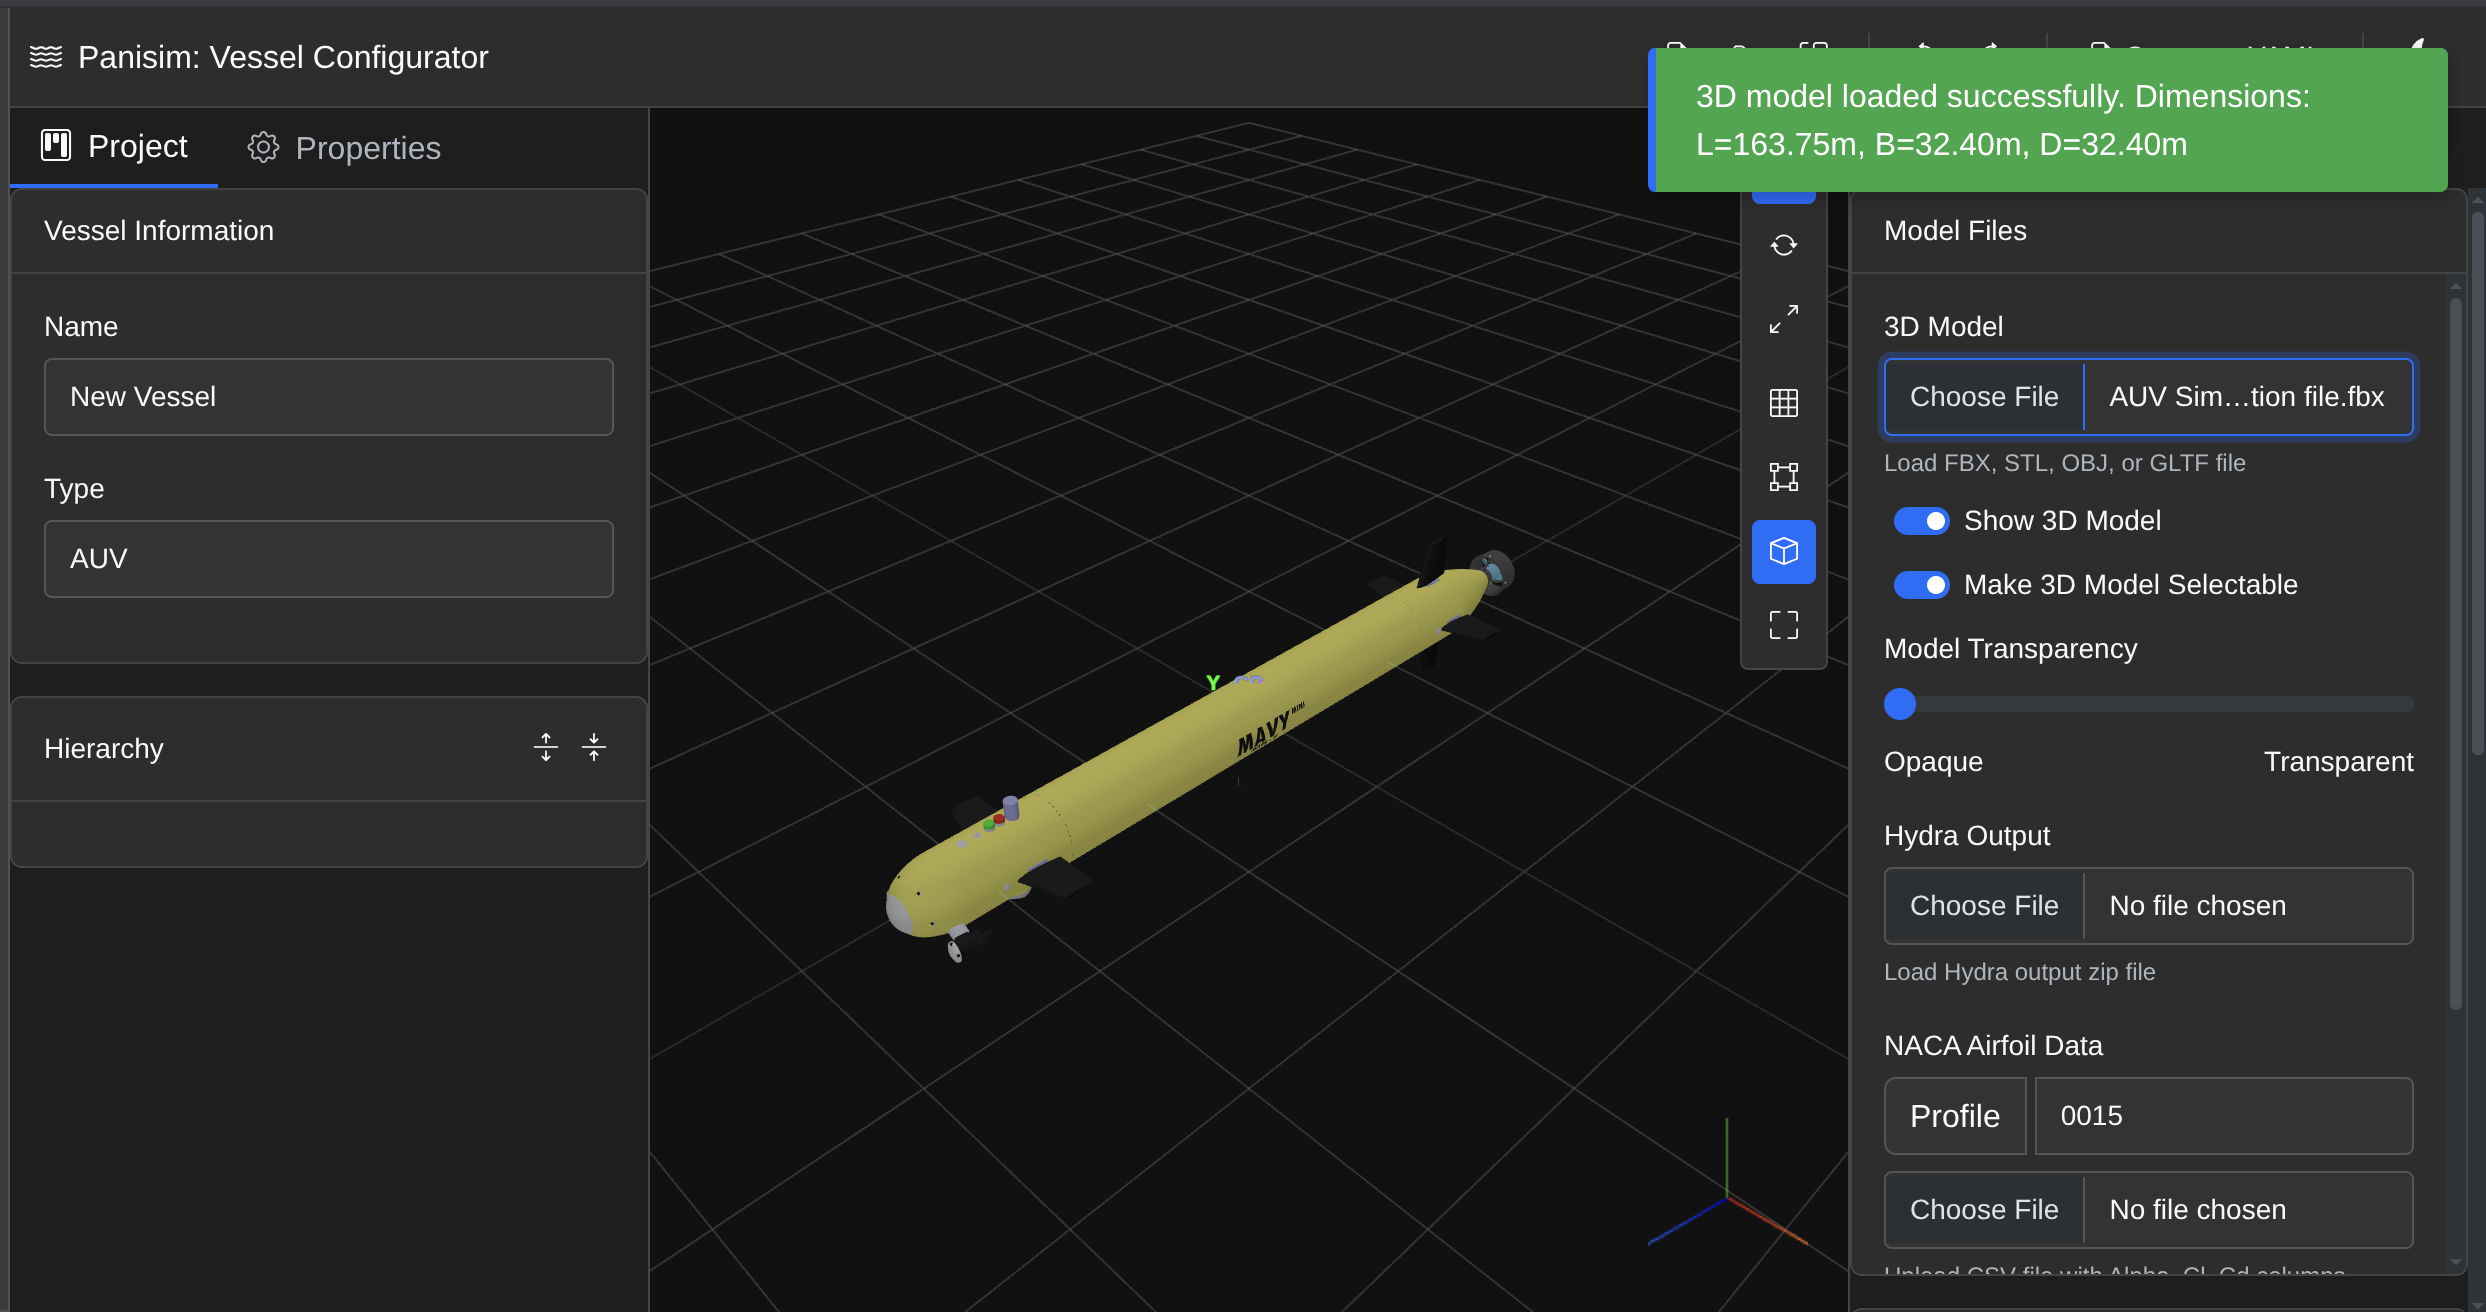
\includegraphics[keepaspectratio]{rawFiles/WebConfigurator/../../images/vesselLoad.png}}

}

\caption{Loaded Vessel}

\end{figure}%

\begin{tcolorbox}[enhanced jigsaw, colback=white, toptitle=1mm, colframe=quarto-callout-tip-color-frame, rightrule=.15mm, breakable, title=\textcolor{quarto-callout-tip-color}{\faLightbulb}\hspace{0.5em}{Tip}, toprule=.15mm, opacitybacktitle=0.6, opacityback=0, coltitle=black, leftrule=.75mm, colbacktitle=quarto-callout-tip-color!10!white, arc=.35mm, titlerule=0mm, bottomtitle=1mm, bottomrule=.15mm, left=2mm]

The software automatically calculates the length, breadth and depth of
the vessel from the FBX file via a bounding box. if possible, you should
have your vessel in the configuration used in marine vessels, i.e X axis
along the length of the vessel pointing forward, Y axis along the
breadth pointing to the starboard and Z axis along the depth pointing
downwards.

\end{tcolorbox}

\subsection*{Step 2: Configure the
Vessel}\label{step-2-configure-the-vessel}
\addcontentsline{toc}{subsection}{Step 2: Configure the Vessel}

\begin{enumerate}
\def\labelenumi{\arabic{enumi}.}
\tightlist
\item
  Select the component (Control Surfaces, Thrusters, or Sensors) you
  want to configure. It will be slightly highlighted on selection.
\end{enumerate}

\begin{figure}[H]

{\centering \pandocbounded{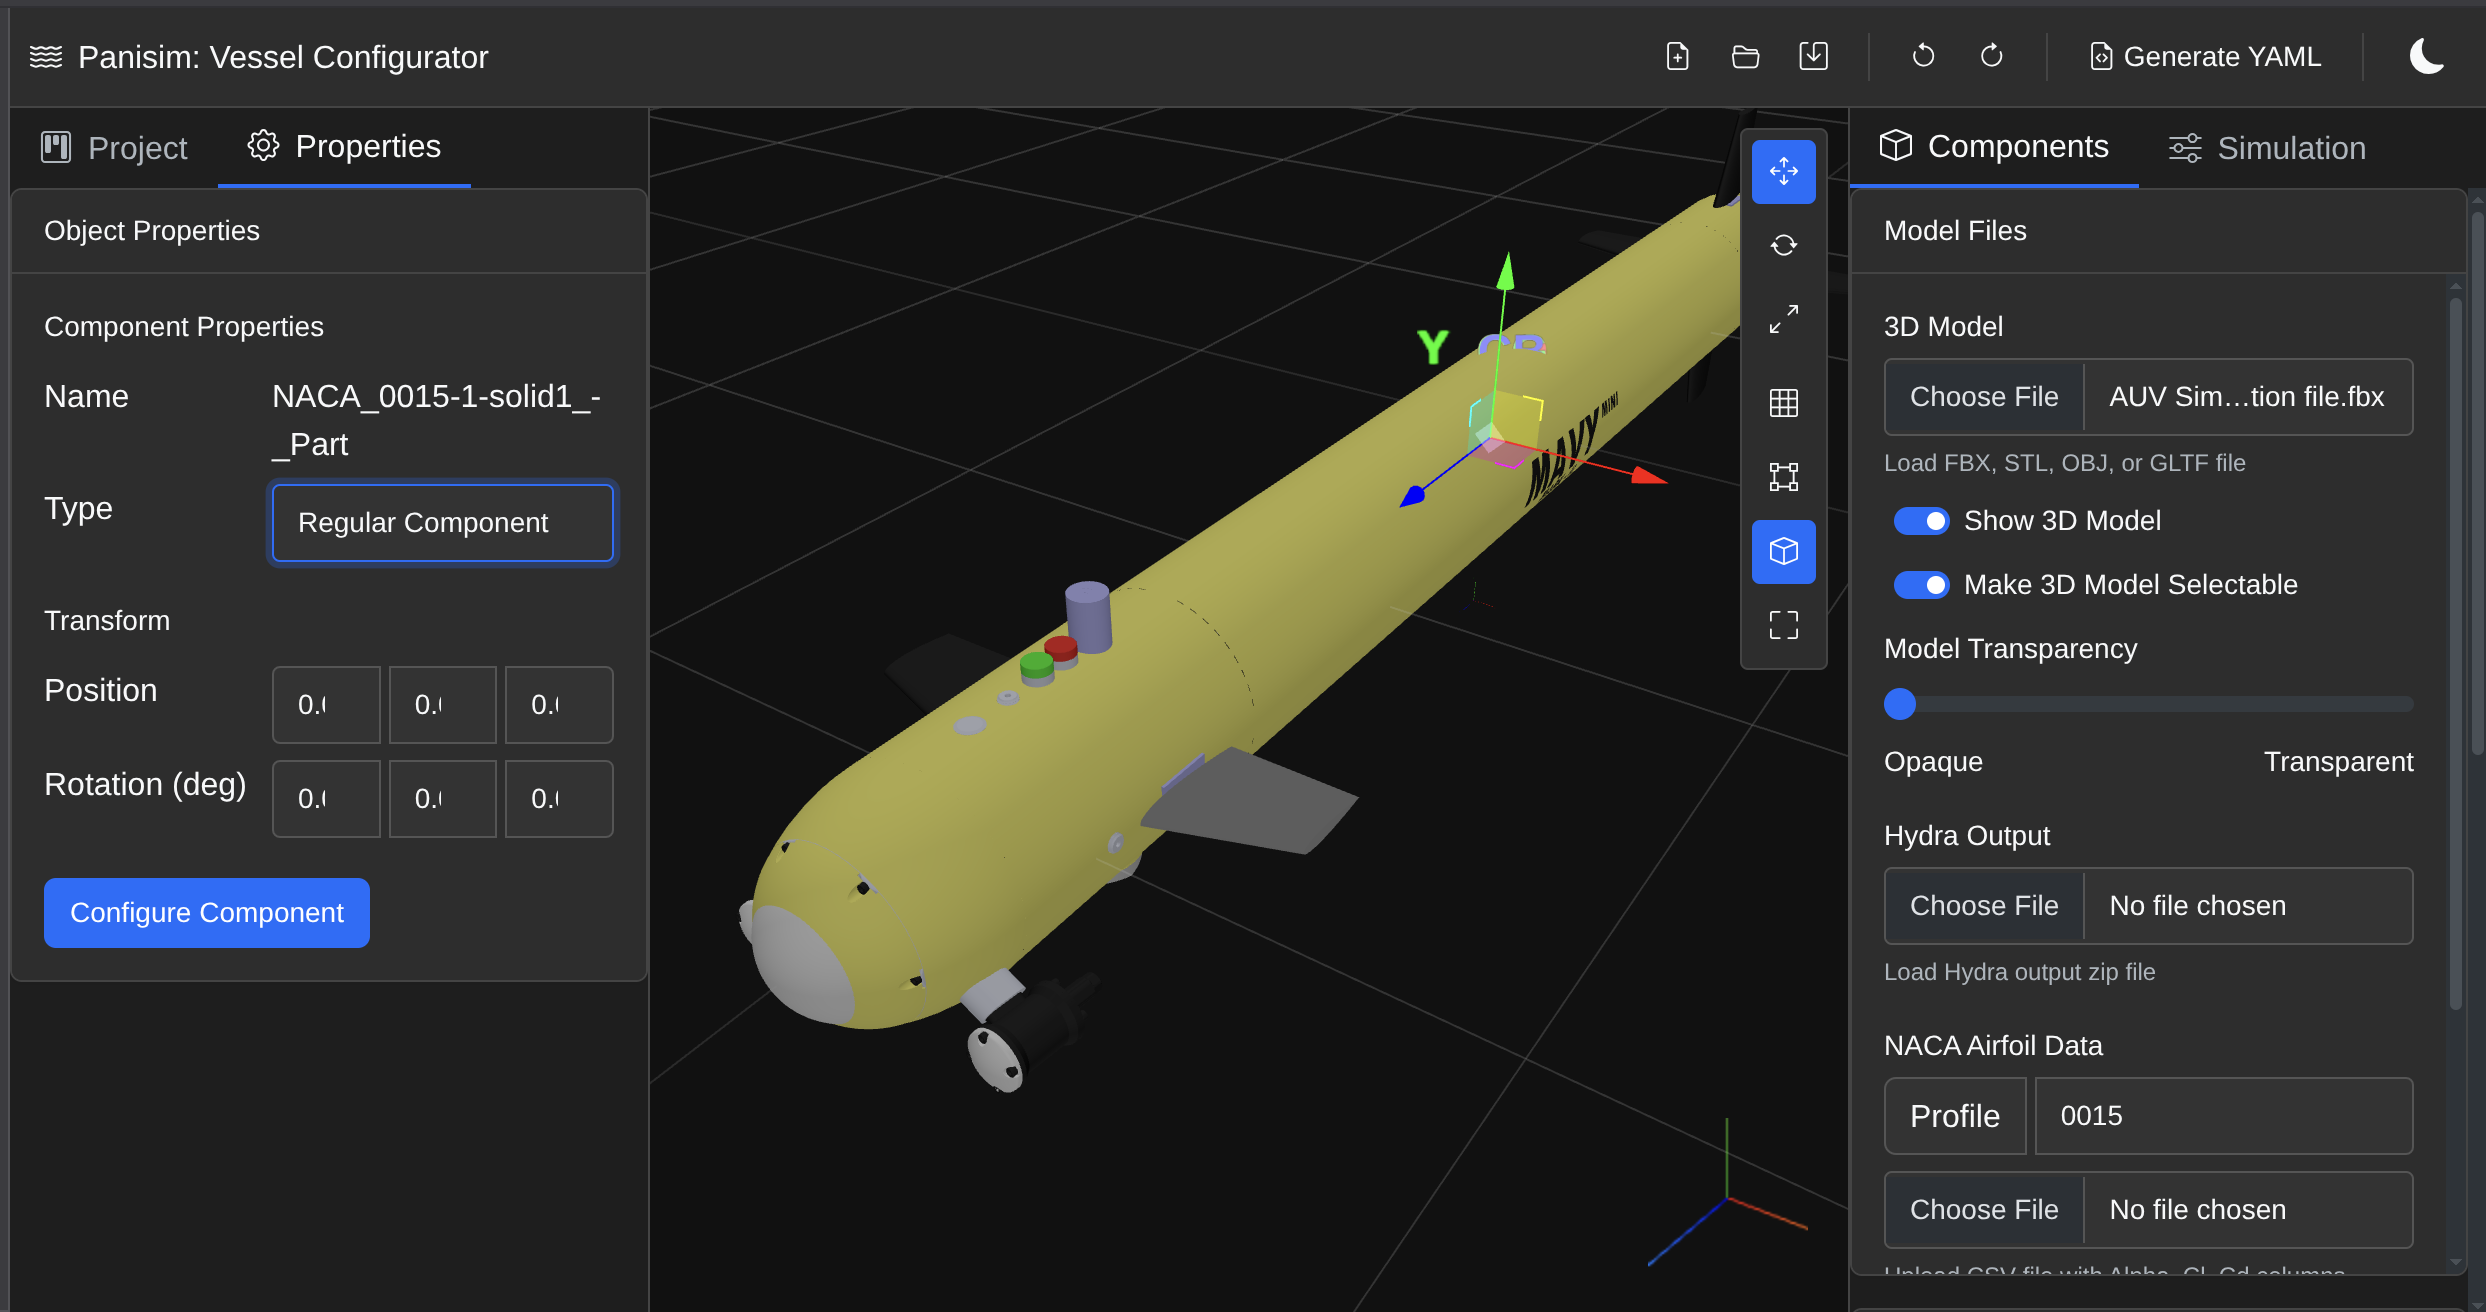
\includegraphics[keepaspectratio]{rawFiles/WebConfigurator/../../images/componentConfig.png}}

}

\caption{Selected Component}

\end{figure}%

\begin{enumerate}
\def\labelenumi{\arabic{enumi}.}
\setcounter{enumi}{1}
\tightlist
\item
  From the left sidebar, switch to the Properties tab and select the
  component type.
\item
  Configuration modal would appear on selecting the component type.
\end{enumerate}

\begin{figure}[H]

{\centering \pandocbounded{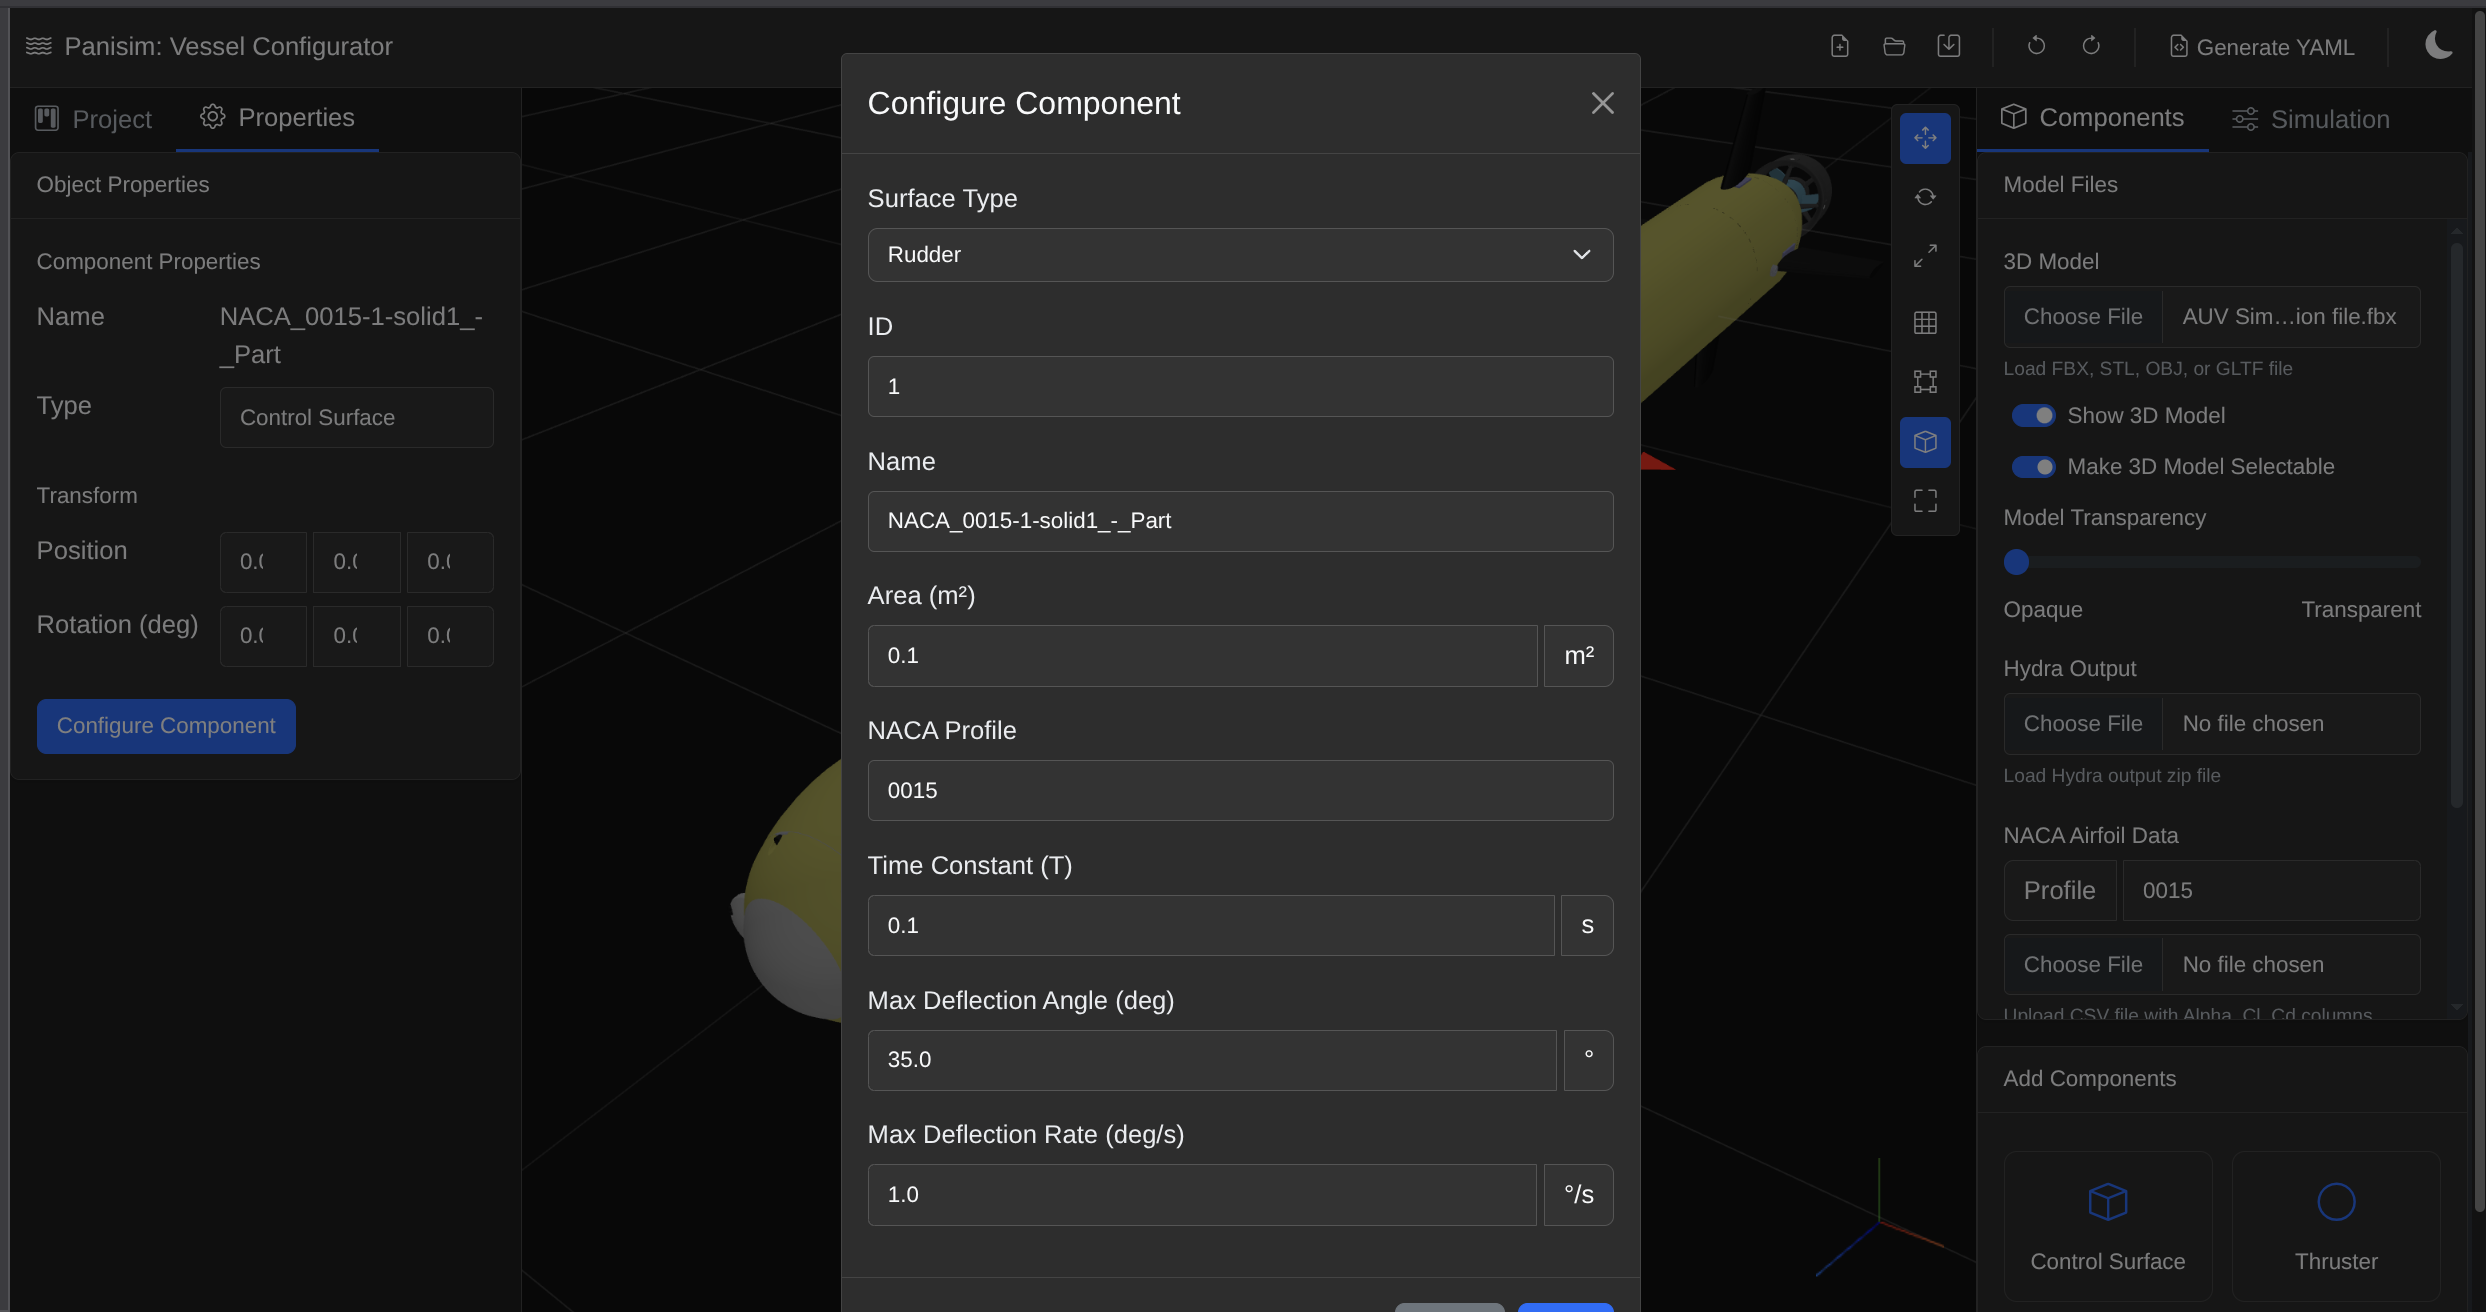
\includegraphics[keepaspectratio]{rawFiles/WebConfigurator/../../images/componentConfig2.png}}

}

\caption{Component Configuration Modal}

\end{figure}%

\begin{enumerate}
\def\labelenumi{\arabic{enumi}.}
\setcounter{enumi}{3}
\tightlist
\item
  Enter the required parameters and click on the ``Apply'' button.
\item
  The component will then be configured. This can be confirmed if you
  see a coordinate system assigned to your vessel.
\end{enumerate}

\begin{figure}[H]

{\centering \pandocbounded{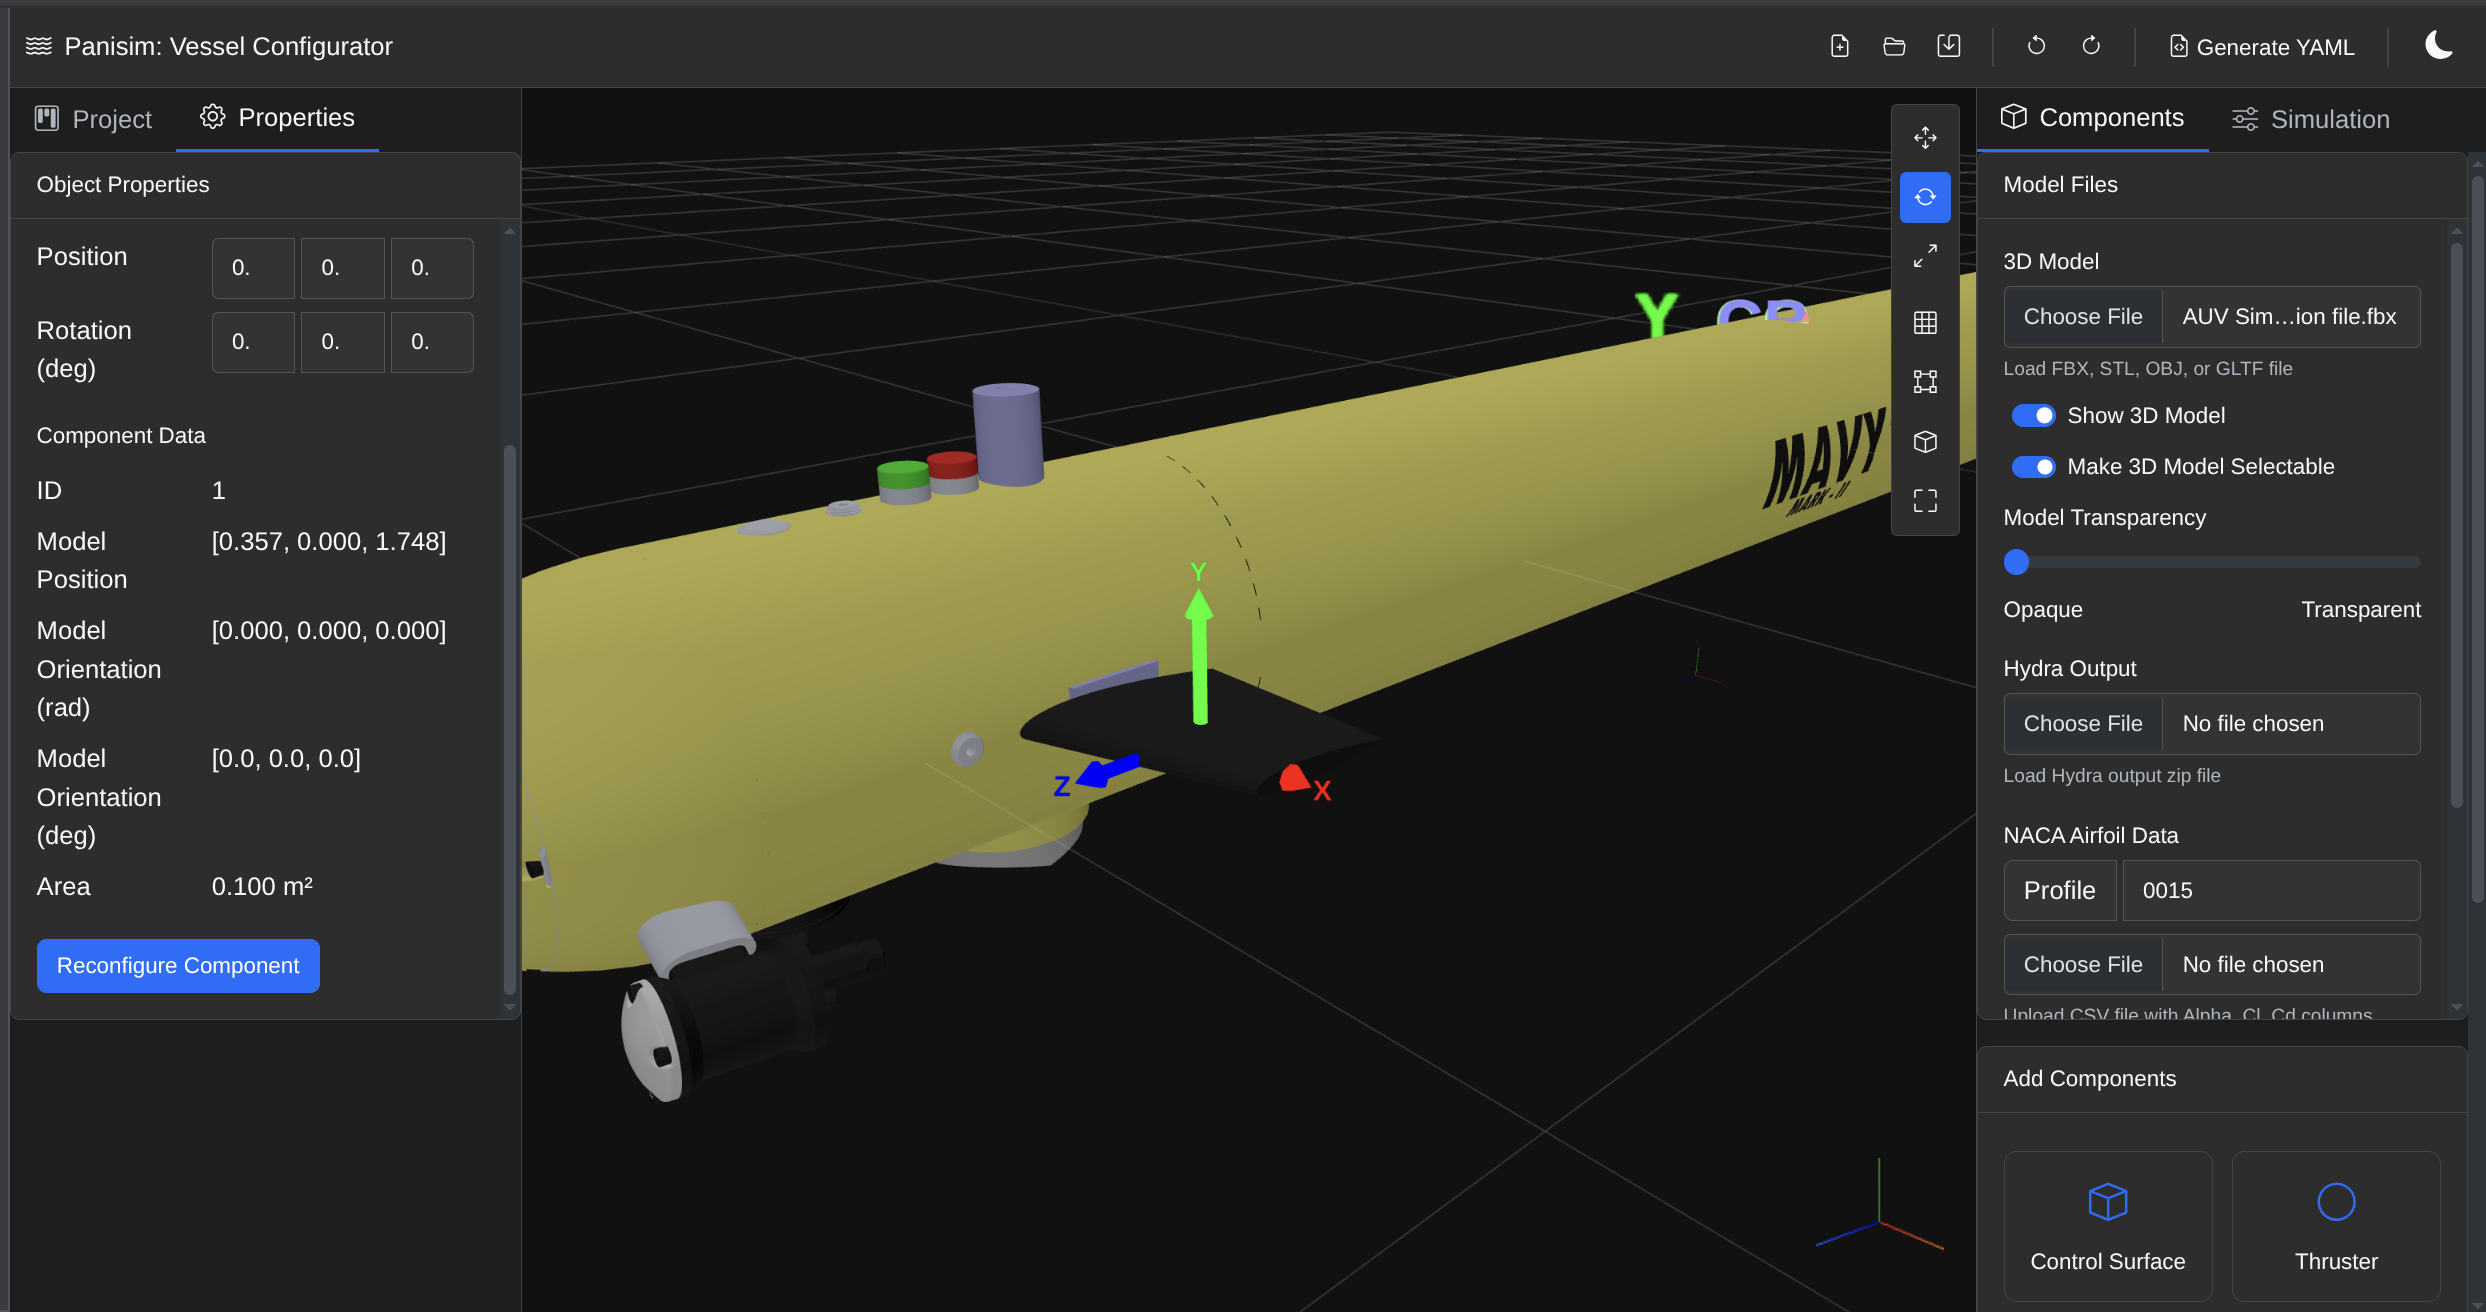
\includegraphics[keepaspectratio]{rawFiles/WebConfigurator/../../images/configuredConfig.png}}

}

\caption{Component Configured}

\end{figure}%

\begin{enumerate}
\def\labelenumi{\arabic{enumi}.}
\setcounter{enumi}{5}
\tightlist
\item
  You should see the position and orientation in the properties tab.
\item
  You can select the coordinate and transform it in the 3D view based on
  where you want to place it.
\end{enumerate}

\begin{figure}[H]

{\centering \pandocbounded{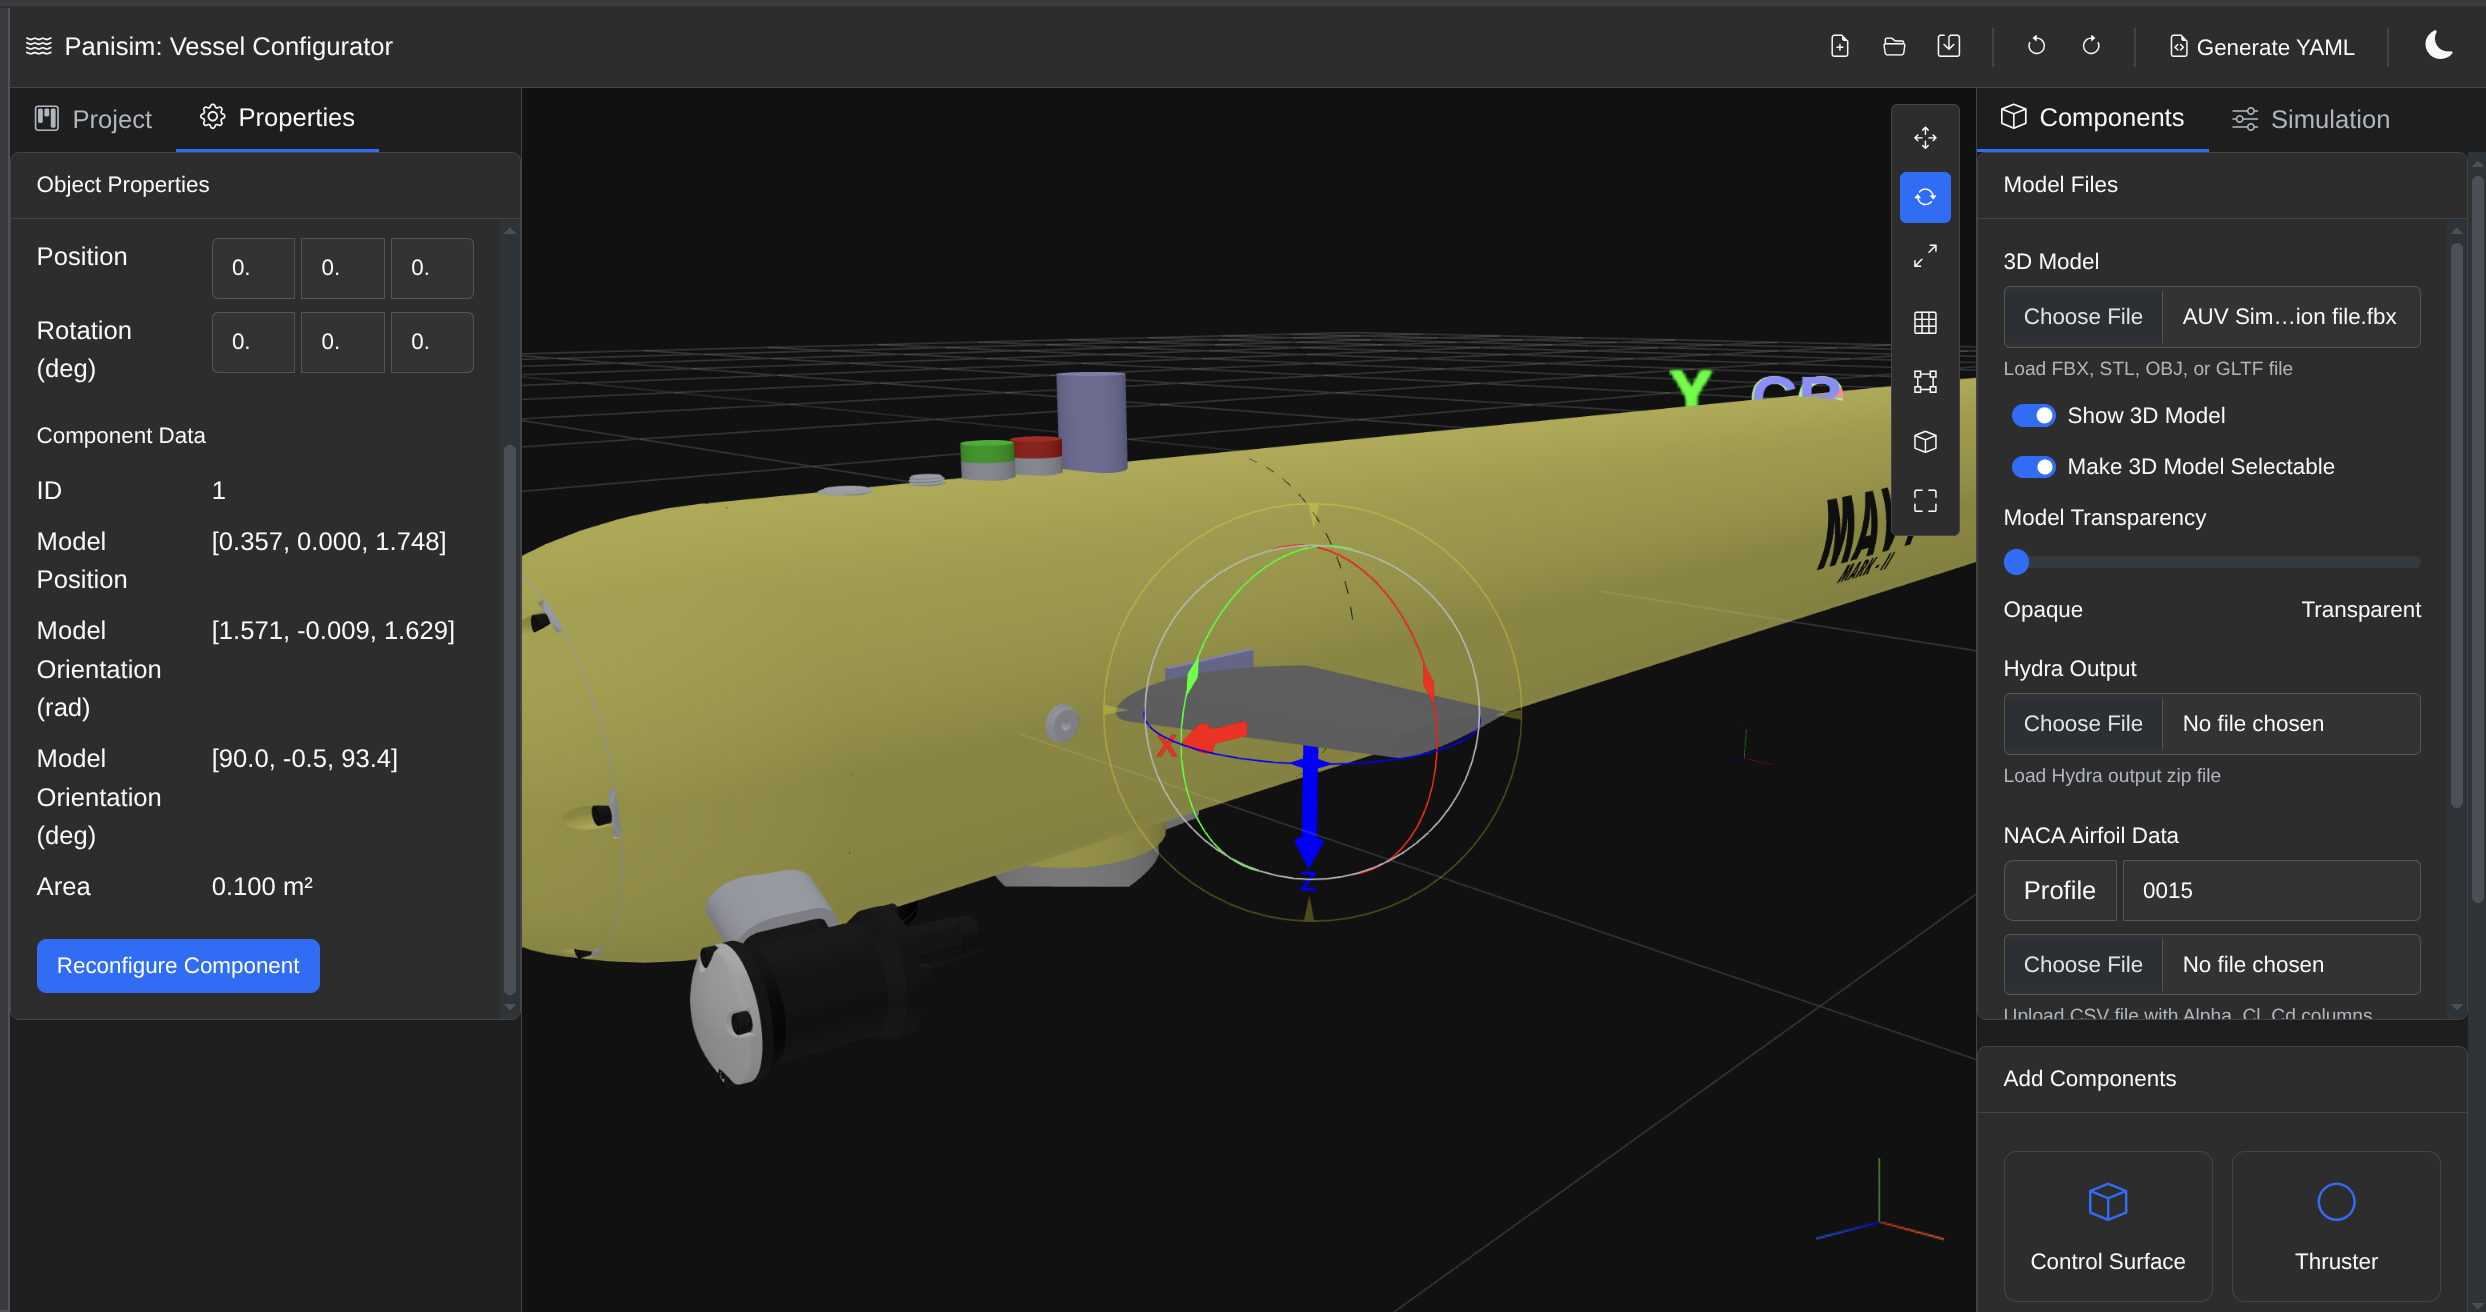
\includegraphics[keepaspectratio]{rawFiles/WebConfigurator/../../images/transformComponent.png}}

}

\caption{Component Configured}

\end{figure}%

For sensors, the orientation have to be how you have mounted it on the
vessel.

For control surfaces, the X axis needs to be along the chord, Y axis
pointing along the span inwards to the vessel and Z axis completing the
right hand coordinate system.

\begin{figure}[H]

{\centering \pandocbounded{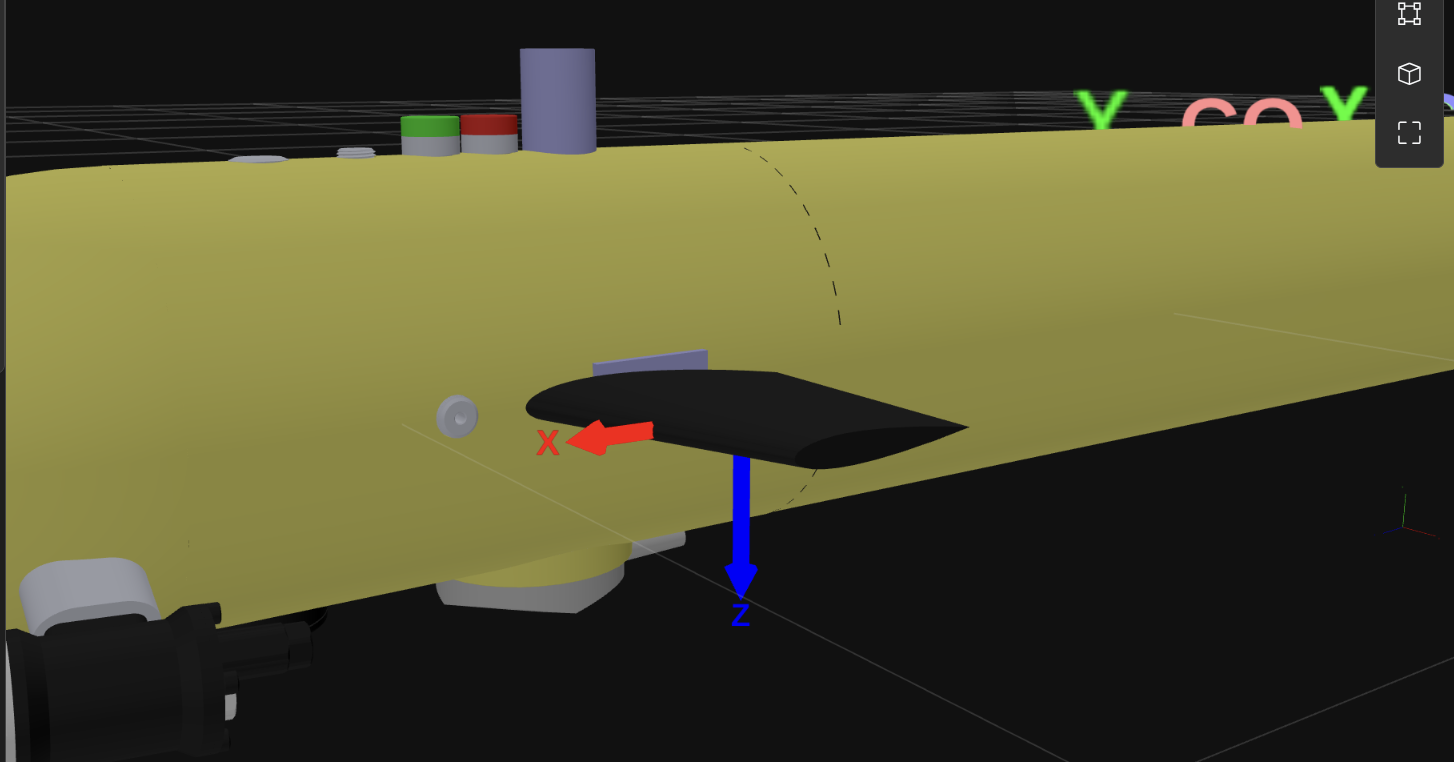
\includegraphics[keepaspectratio]{rawFiles/WebConfigurator/../../images/controlSurfaceConfig.png}}

}

\caption{Control Surface}

\end{figure}%

For thrusters, the X axis needs to be along the axis of the thruster, Y
axis pointing towards the starboard and Z axis completing the right hand
coordinate system.

Everything follows the NED (North, East, Down) coordinate system.

\subsection*{Step 3: Placing the vessel center
points}\label{step-3-placing-the-vessel-center-points}
\addcontentsline{toc}{subsection}{Step 3: Placing the vessel center
points}

\begin{enumerate}
\def\labelenumi{\arabic{enumi}.}
\tightlist
\item
  Make the vessel transparent to see the inside. And untoggle the ``Make
  3D Model Selectable'' option. This will allow you to select the centre
  points and transform them.
\end{enumerate}

\begin{figure}[H]

{\centering \pandocbounded{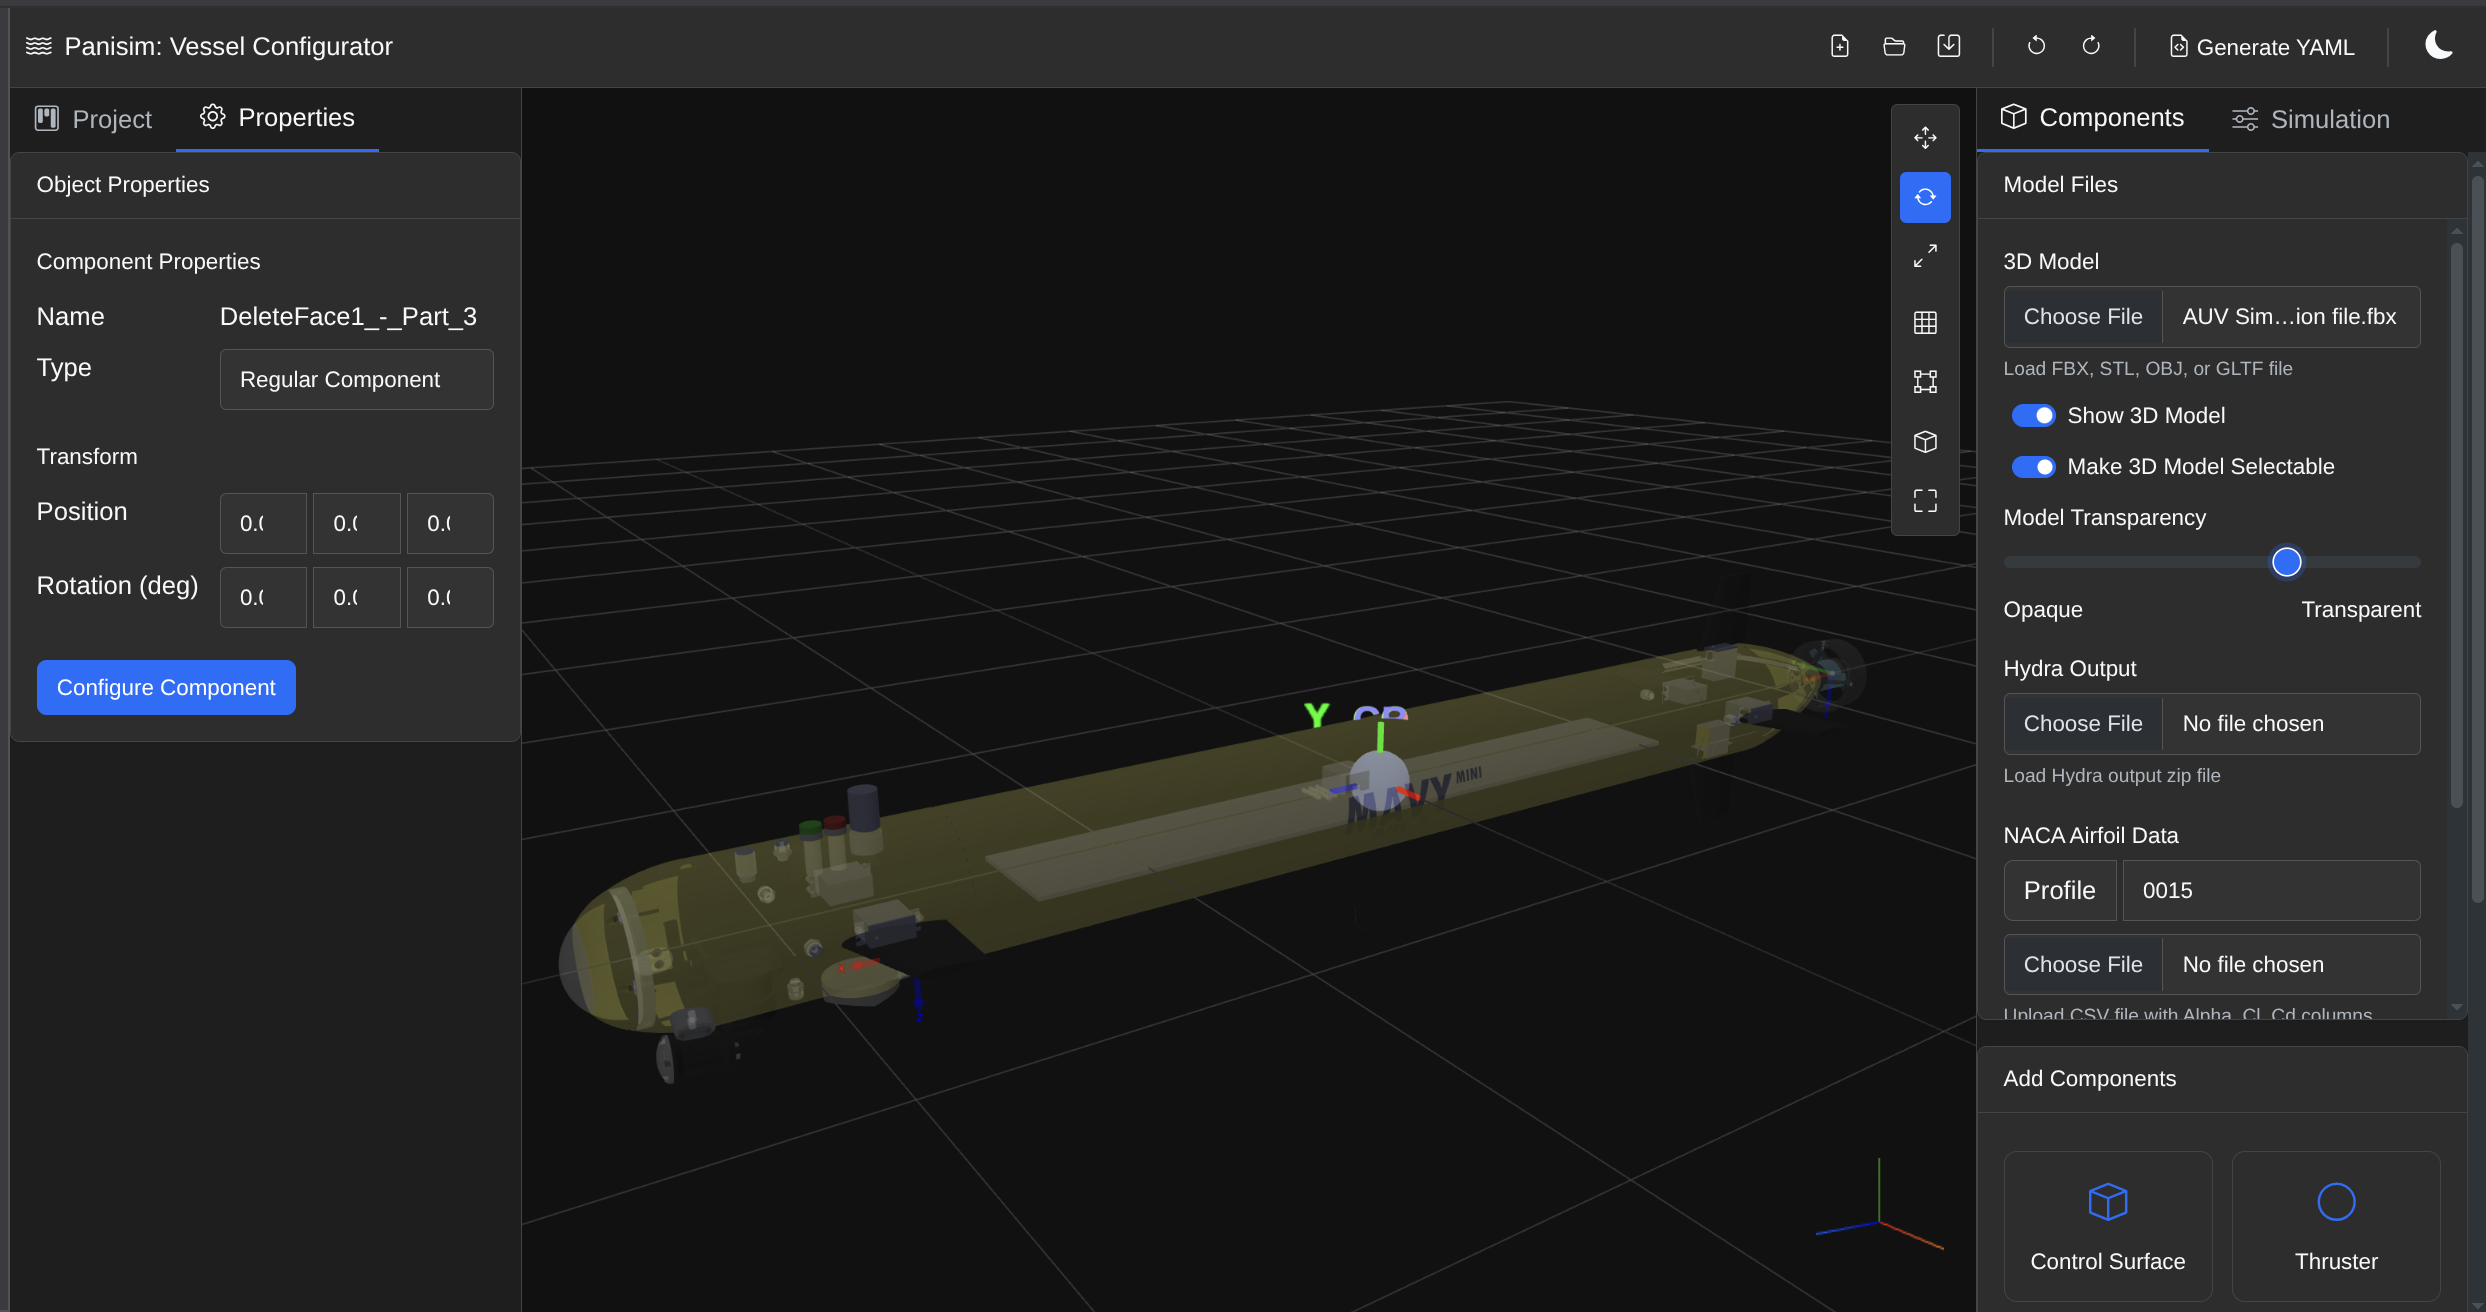
\includegraphics[keepaspectratio]{rawFiles/WebConfigurator/../../images/transparentModel.png}}

}

\caption{Transparent Vessel}

\end{figure}%

\begin{enumerate}
\def\labelenumi{\arabic{enumi}.}
\setcounter{enumi}{1}
\tightlist
\item
  You can select each of the center points and transform them to the
  desired location.
\item
  You can also manually enter the coordinates in the
  \texttt{Edit\ Geometry\ Parameters} in the right sidebar components
  tab.
\item
  The Body Centre {[}CO{]}, is the point with respect to which all other
  coordinates are defined. And therefore it must be placed in the NED
  configuration.
\end{enumerate}

\subsection*{Step 4: Edit Hydrodynamic
Coefficients}\label{step-4-edit-hydrodynamic-coefficients}
\addcontentsline{toc}{subsection}{Step 4: Edit Hydrodynamic
Coefficients}

\begin{enumerate}
\def\labelenumi{\arabic{enumi}.}
\tightlist
\item
  Edit the hydrodynamic coefficients in the
  \texttt{Edit\ Hydrodynamic\ Coefficients} in the right sidebar
  components tab. Follow the instructions in the modal to enter the
  hydrodynamic coefficients.
\end{enumerate}

\begin{figure}[H]

{\centering \pandocbounded{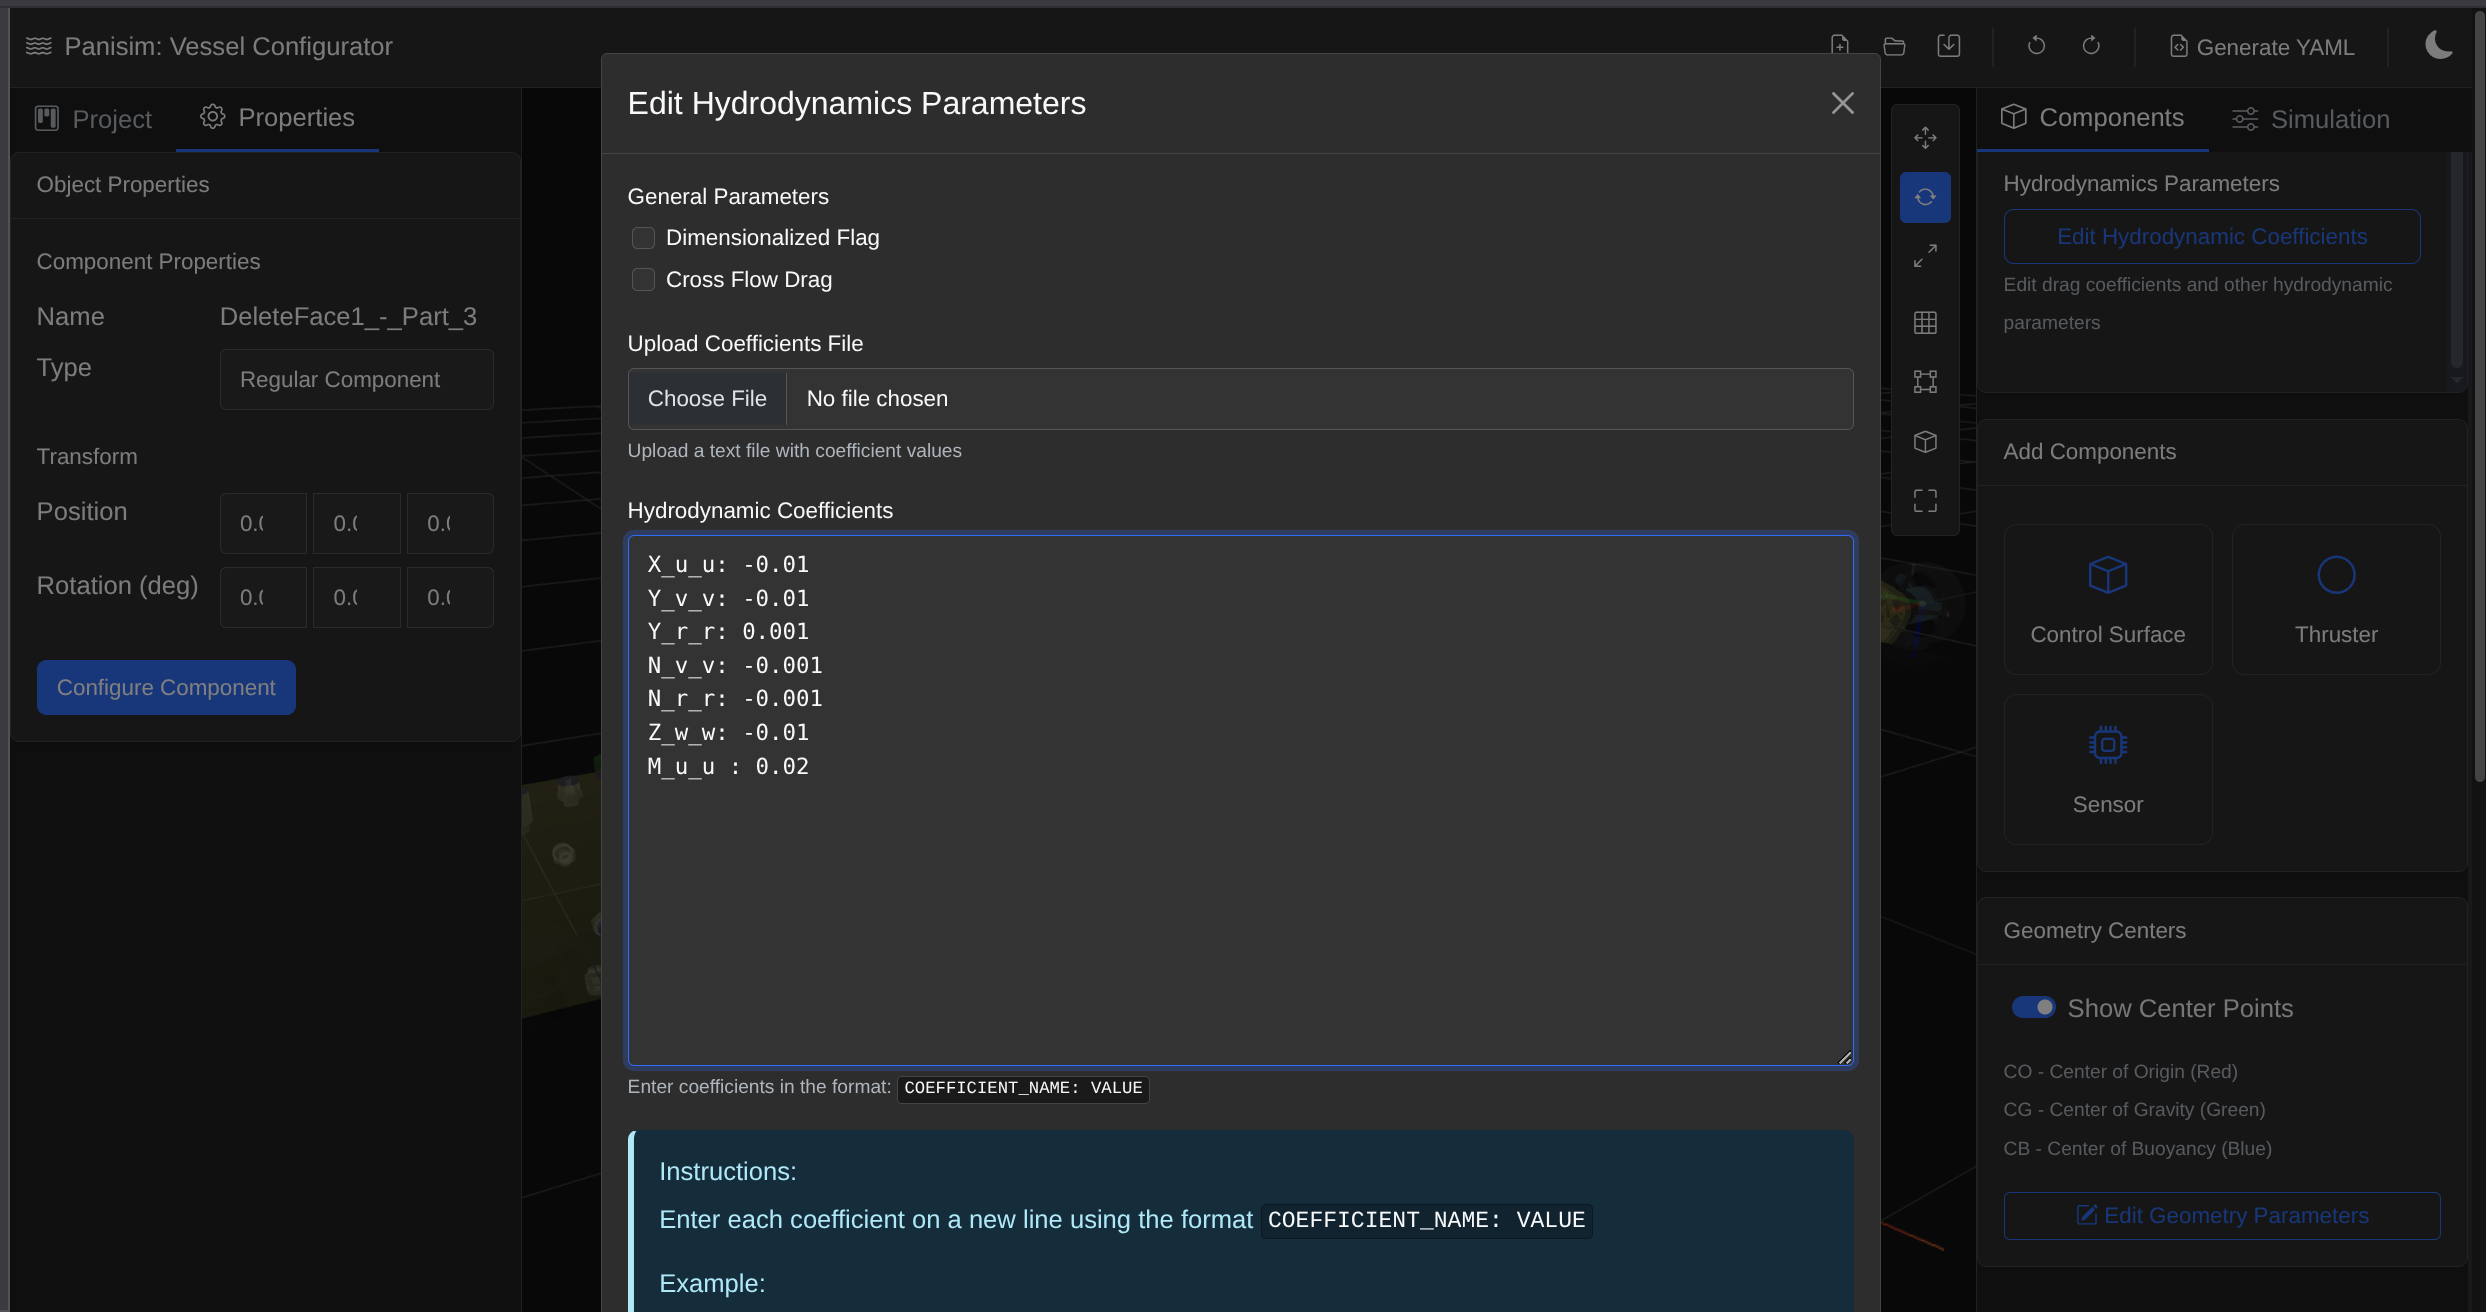
\includegraphics[keepaspectratio]{rawFiles/WebConfigurator/../../images/hydroConfig.png}}

}

\caption{Hydrodynamic Coefficients}

\end{figure}%

\subsection*{Step 5: Simulation
settings}\label{step-5-simulation-settings}
\addcontentsline{toc}{subsection}{Step 5: Simulation settings}

\begin{enumerate}
\def\labelenumi{\arabic{enumi}.}
\tightlist
\item
  Edit all the parameters in the \texttt{Simulation} tab in the right
  sidebar.
\end{enumerate}

\begin{tcolorbox}[enhanced jigsaw, colback=white, toptitle=1mm, colframe=quarto-callout-note-color-frame, rightrule=.15mm, breakable, title=\textcolor{quarto-callout-note-color}{\faInfo}\hspace{0.5em}{Note}, toprule=.15mm, opacitybacktitle=0.6, opacityback=0, coltitle=black, leftrule=.75mm, colbacktitle=quarto-callout-note-color!10!white, arc=.35mm, titlerule=0mm, bottomtitle=1mm, bottomrule=.15mm, left=2mm]

In the \texttt{Advanced\ Simualtion\ Parameters}, you can visually
select the geofence boundaries. This also can be further extended to
select waypoints in a future release.

\end{tcolorbox}

\begin{figure}[H]

{\centering \pandocbounded{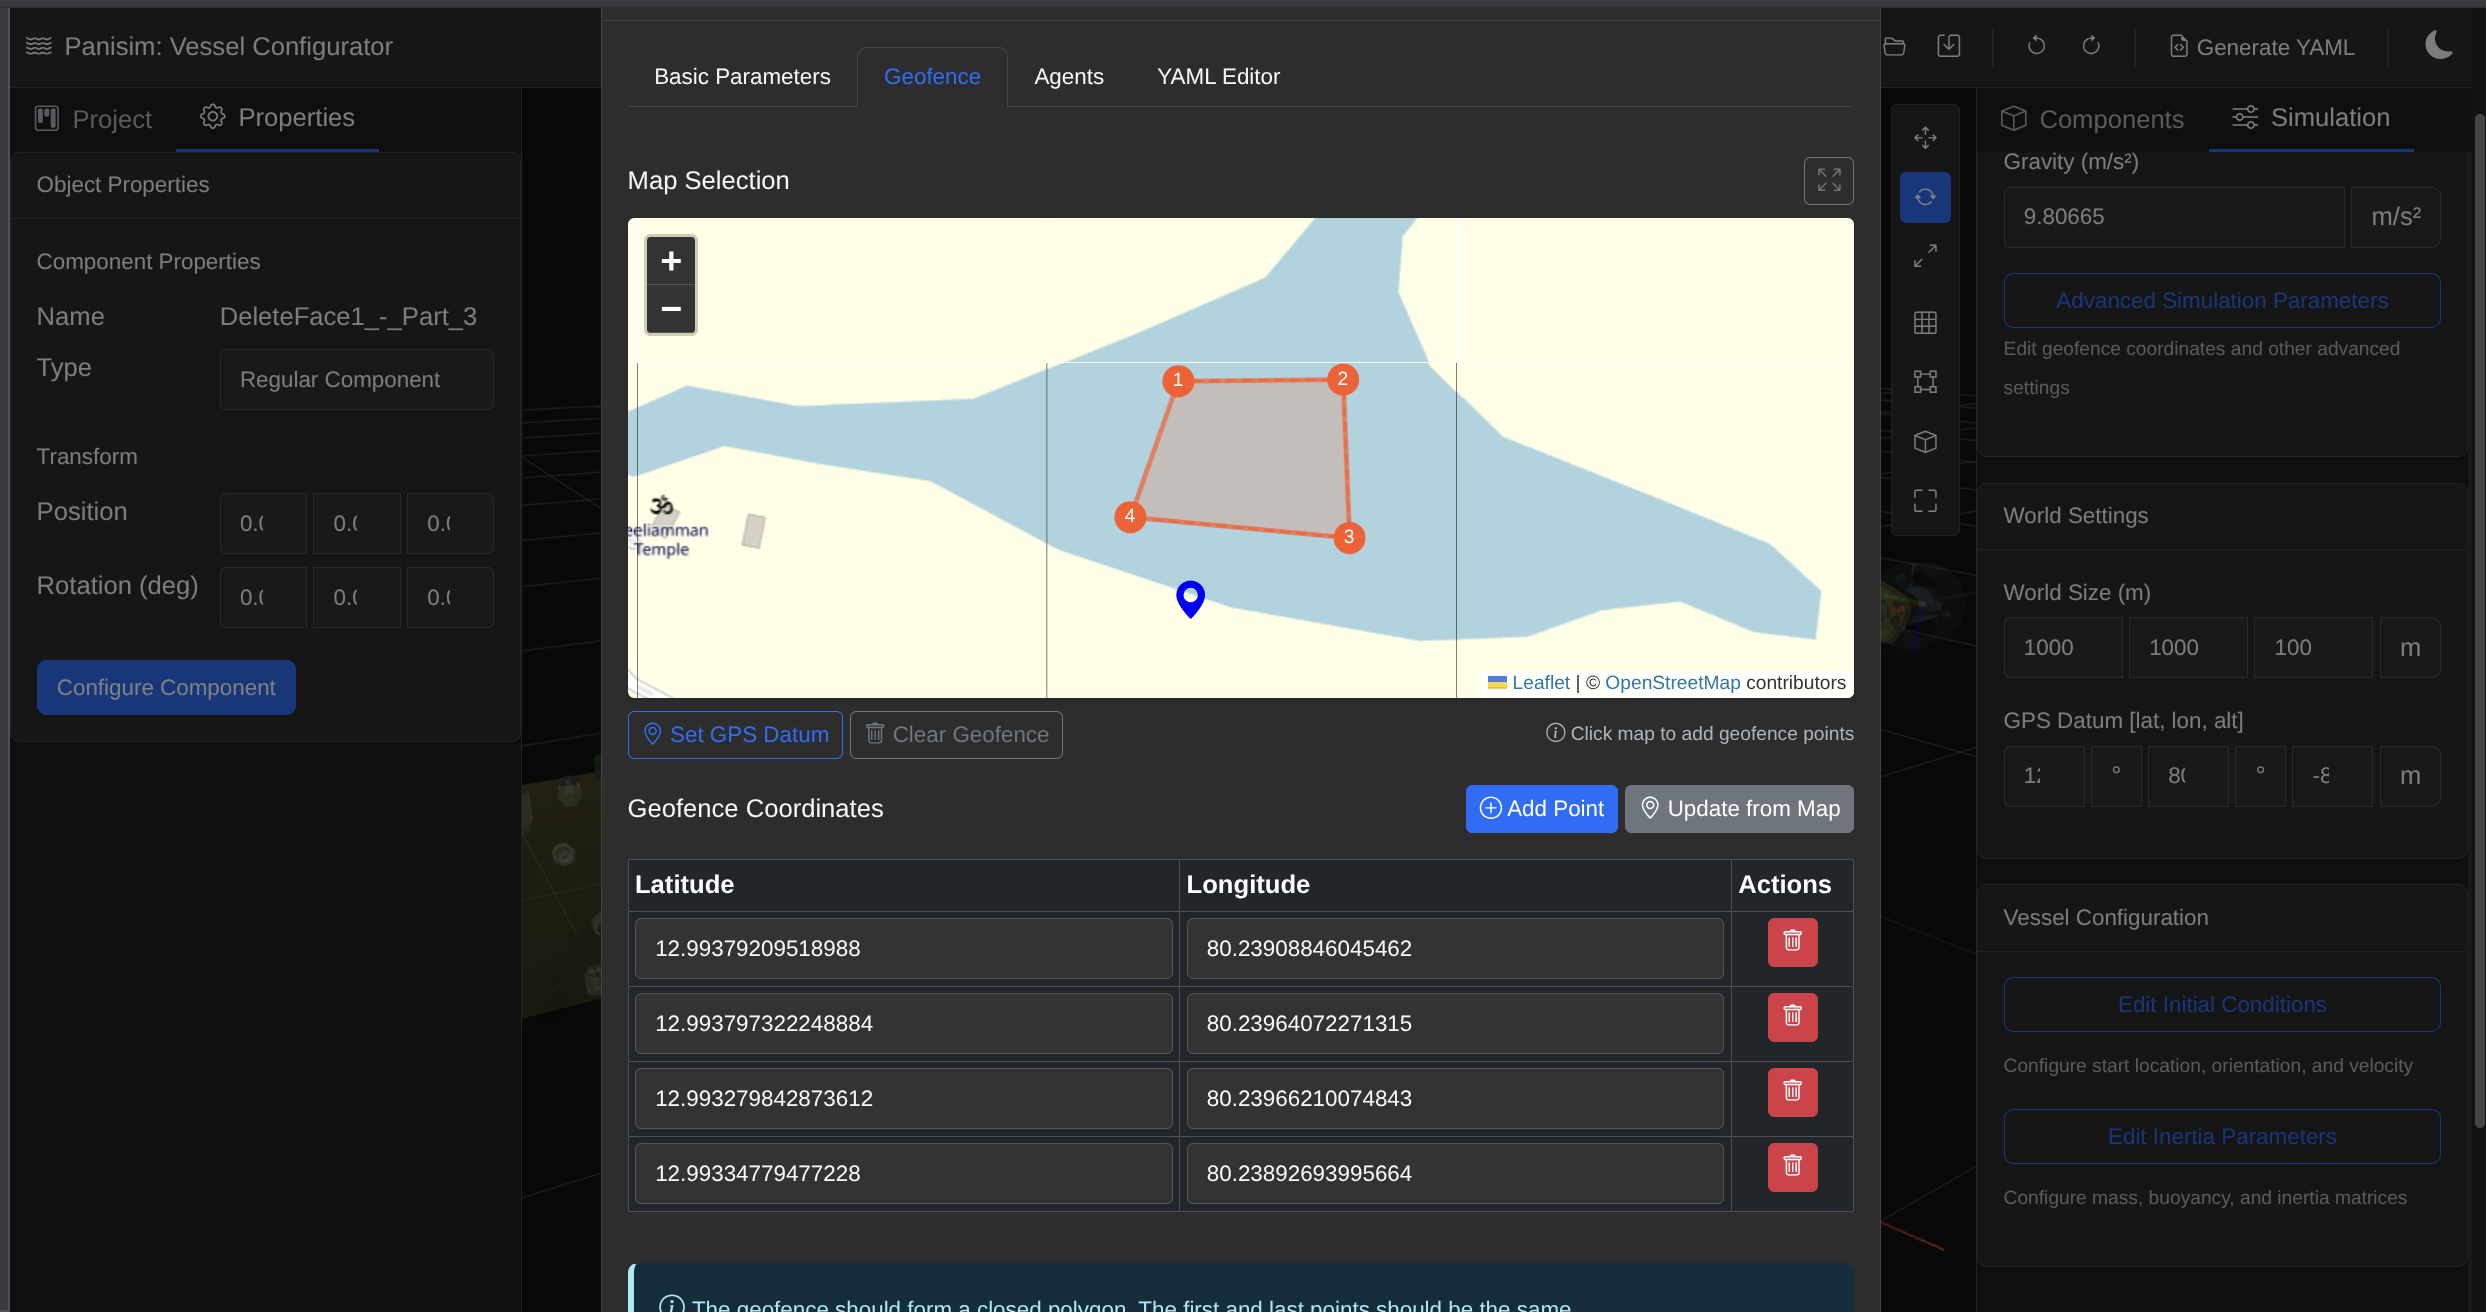
\includegraphics[keepaspectratio]{rawFiles/WebConfigurator/../../images/GeofenceConfig.png}}

}

\caption{Geofence}

\end{figure}%

\subsection*{Step 6: Upload the Hydra output file (optional, if you are
not using cross-flow
drag)}\label{step-6-upload-the-hydra-output-file-optional-if-you-are-not-using-cross-flow-drag}
\addcontentsline{toc}{subsection}{Step 6: Upload the Hydra output file
(optional, if you are not using cross-flow drag)}

You can get your Hydra output file from the \href{}{HydRA website}. And
upload the zip folder in the web gui. The generated input file will then
contain your Hydra file with correct path.

\subsection*{Step 7: Generate the YAML
files}\label{step-7-generate-the-yaml-files}
\addcontentsline{toc}{subsection}{Step 7: Generate the YAML files}

\begin{enumerate}
\def\labelenumi{\arabic{enumi}.}
\tightlist
\item
  Click on the ``Generate YAML'' button in the toolbar.
\item
  The YAML files will be generated and downloaded as a zip file.
\item
  Unzip the file and place it in the \texttt{inputs} directory.
\end{enumerate}

And there you have it! You have successfully configured your vessel and
generated the required input files for the Panisim simulator. Some
configuration file may require manual edits. Feel free to play around
with the Web GUI and extend its functionality.

\section*{Software Architecture}\label{software-architecture}
\addcontentsline{toc}{section}{Software Architecture}

\markright{Software Architecture}

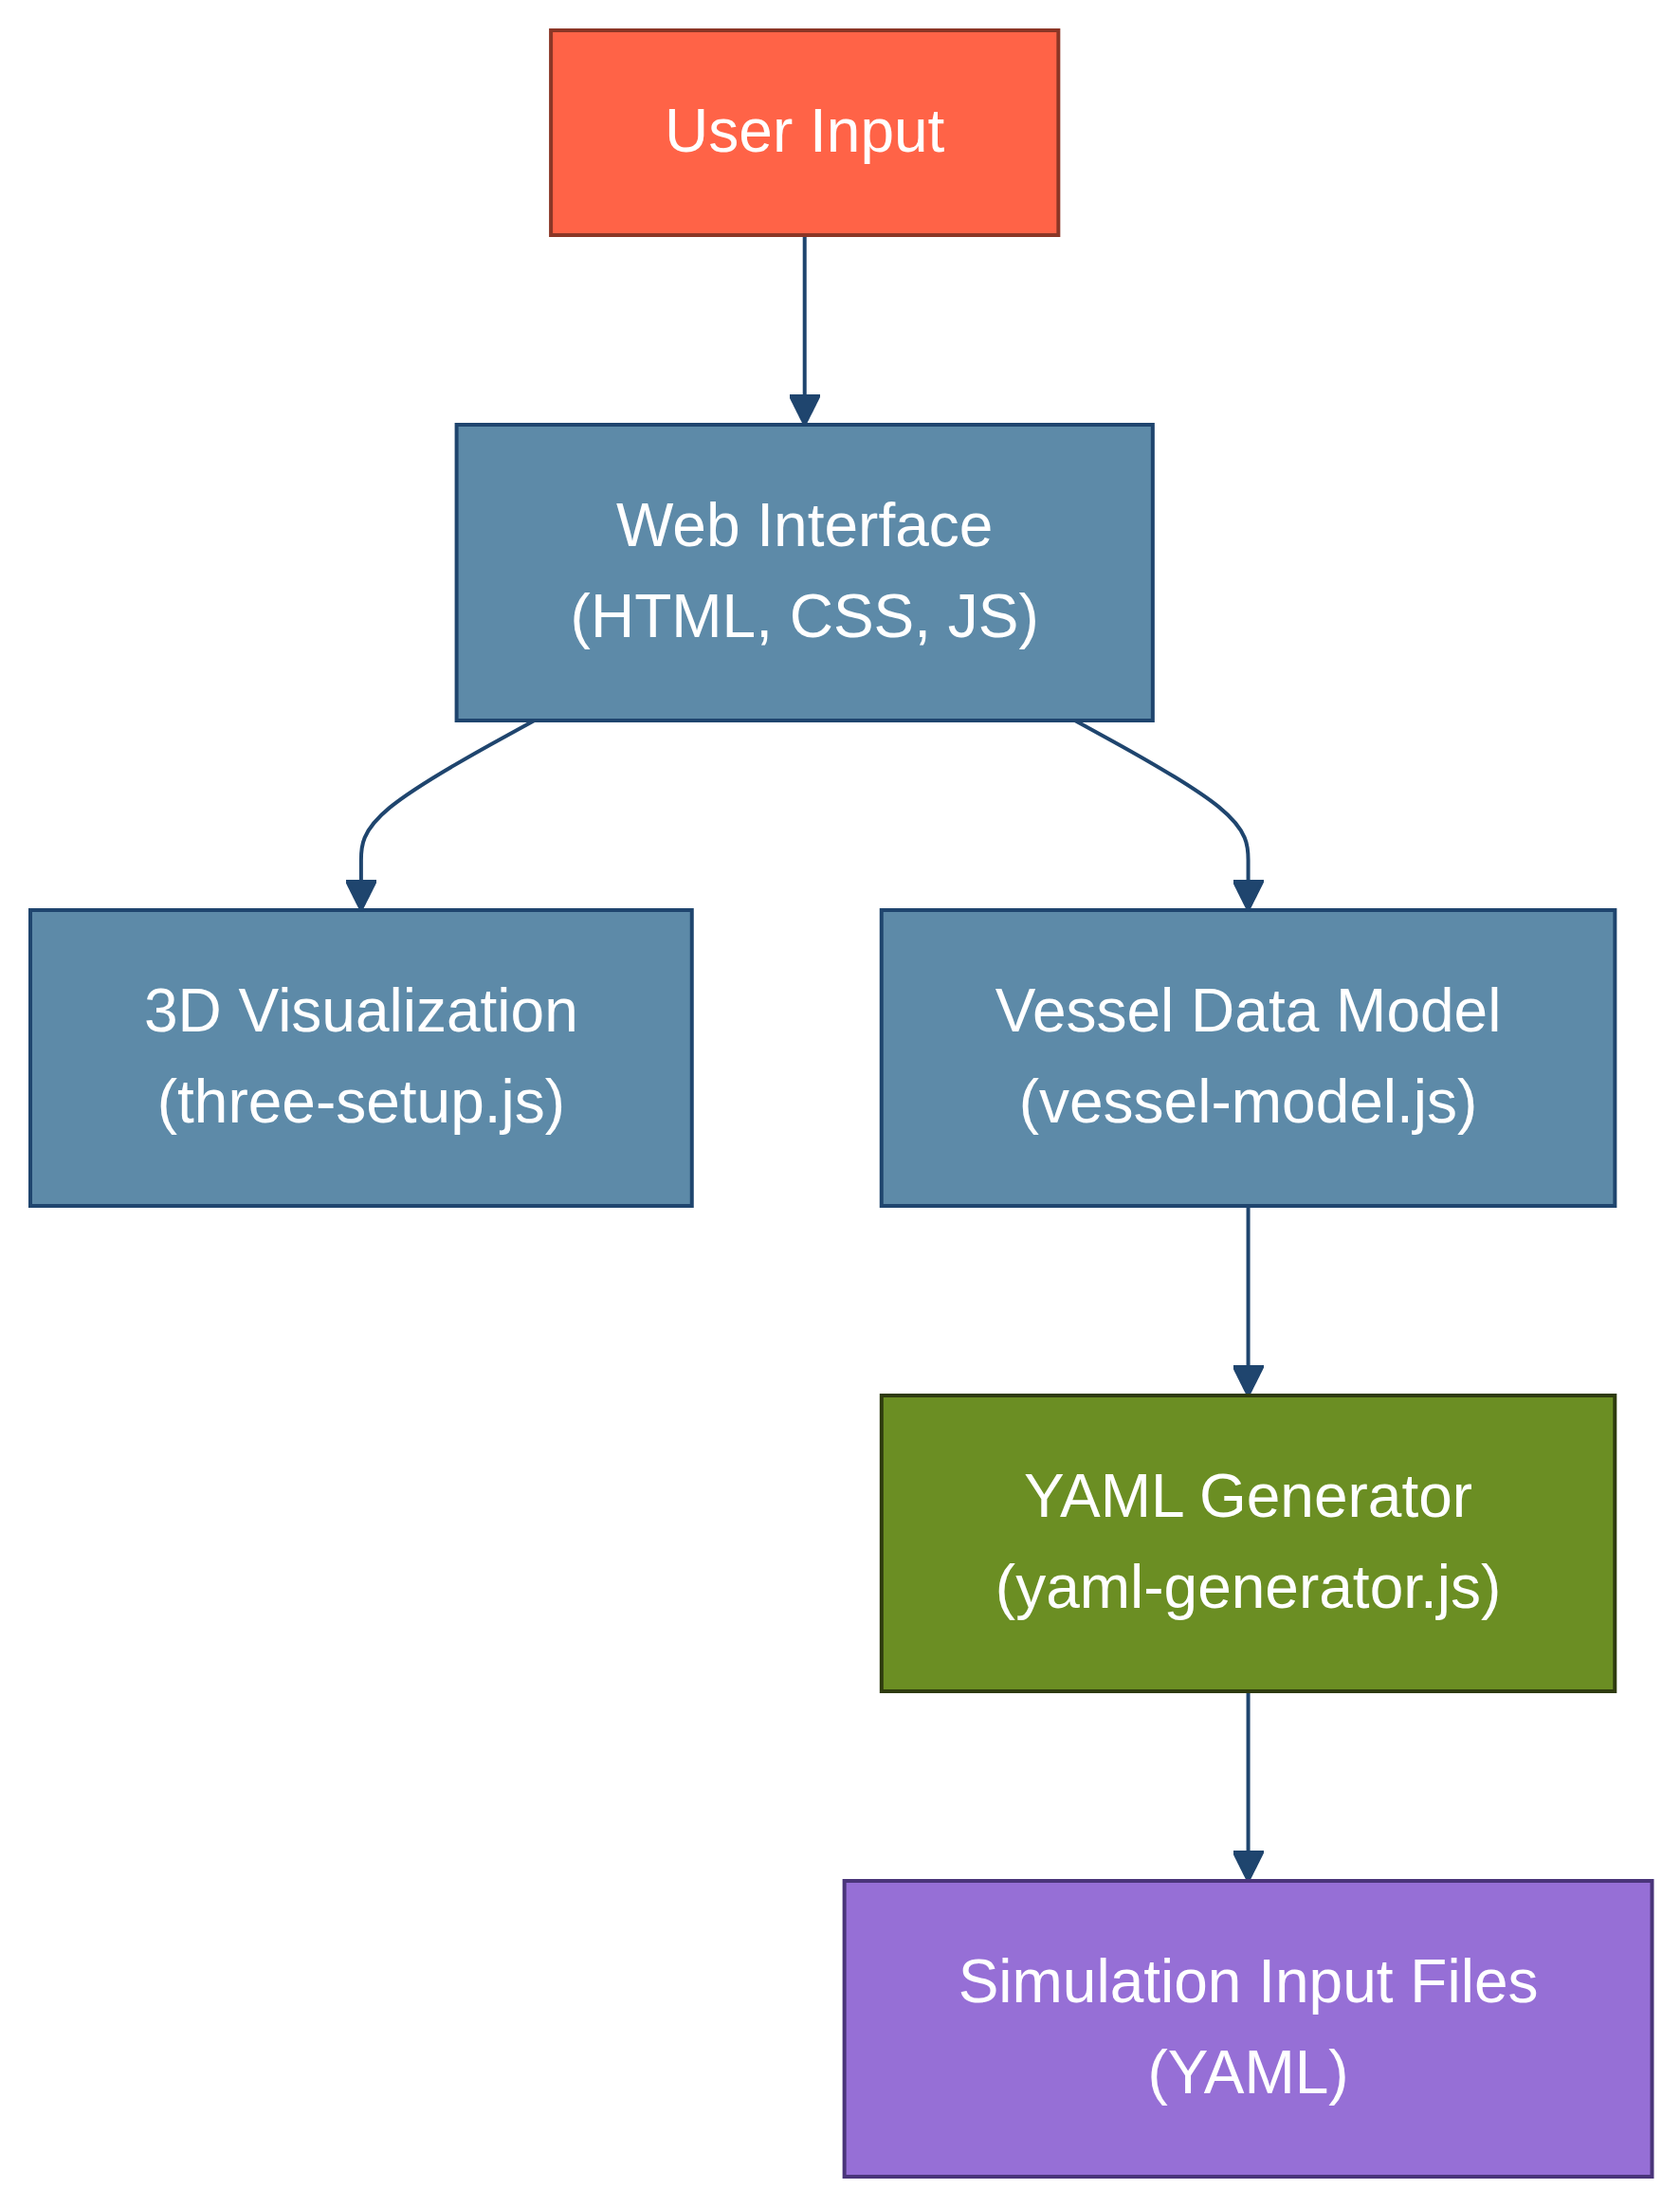
\includegraphics[width=4.62in,height=6.06in]{rawFiles/WebConfigurator/web_configurator_files/figure-latex/mermaid-figure-1.png}

The Vessel Configurator provides a complete workflow for creating and
configuring marine vessels with the following key features:

\begin{itemize}
\tightlist
\item
  \textbf{Parameter Configuration}: Intuitive interfaces for setting
  physical properties and simulation parameters, GPS waypoints.
\item
  \textbf{Component Management}: Add, edit, and position thrusters,
  control surfaces, and sensors
\item
  \textbf{YAML Generation}: Automatic generation of properly formatted
  configuration files for the simulator
\item
  \textbf{Validation}: Built-in checks to ensure valid component ID
  configuration
\end{itemize}

\subsection*{Core Components}\label{core-components}
\addcontentsline{toc}{subsection}{Core Components}

\begin{enumerate}
\def\labelenumi{\arabic{enumi}.}
\tightlist
\item
  \textbf{User Interface (\texttt{index.html}, \texttt{styles.css},
  \texttt{themes.css})}

  \begin{itemize}
  \tightlist
  \item
    Implements a responsive, CAD-style interface with Bootstrap 5.3.2
    framework integration
  \item
    Features a component hierarchy with:

    \begin{itemize}
    \tightlist
    \item
      Primary toolbar containing application controls
      (new/load/save/undo/redo)
    \item
      Split-pane workspace with resizable panels using Split.js
    \item
      Left sidebar with tabbed project explorer and properties inspector
    \item
      3D viewport with transform controls and visualization options
    \item
      Right sidebar with component addition and configuration panels
    \item
      Modal dialogs for advanced configuration options and YAML preview
    \end{itemize}
  \item
    Supports context-sensitive property editing with dynamic form
    generation
  \item
    Implements theme switching functionality with CSS variables for
    light/dark modes
  \item
    Maintains responsive layout through Bootstrap grid system and custom
    flex containers
  \end{itemize}
\item
  \textbf{3D Visualization Engine (\texttt{three-setup.js})}

  \begin{itemize}
  \tightlist
  \item
    Implements a Three.js-based rendering system with WebGL acceleration
  \item
    Configures high-performance renderer with antialiasing, physically
    correct lighting, and shadow mapping
  \item
    Manages scene graph with hierarchical component structure and
    parent-child relationships
  \item
    Features multiple coordinate systems (world, vessel-local,
    component-local)
  \item
    Implements interactive controls with:

    \begin{itemize}
    \tightlist
    \item
      OrbitControls for camera navigation (pan, rotate, zoom)
    \item
      TransformControls for direct manipulation (translate, rotate,
      scale)
    \item
      Raycaster-based object selection with visual feedback
    \end{itemize}
  \item
    Provides real-time synchronization between 3D objects and data model
    properties
  \item
    Implements custom visual feedback systems including:

    \begin{itemize}
    \tightlist
    \item
      Color-coded component highlighting for selection state
    \item
      Local axes visualization for component orientation
    \item
      Text sprite labeling for identification and measurements
    \item
      Dynamic material updates for selection and hover states
    \end{itemize}
  \item
    Optimizes rendering performance using:

    \begin{itemize}
    \tightlist
    \item
      Request animation frame with conditional rendering
    \item
      Efficient mesh creation with geometry instancing
    \item
      Adaptive resolution scaling based on device capabilities
    \item
      Conditional shadow casting based on object importance
    \end{itemize}
  \end{itemize}
\item
  \textbf{Vessel Data Model (\texttt{vessel-model.js})}

  \begin{itemize}
  \tightlist
  \item
    Implements a comprehensive object-oriented data structure with 1156+
    lines of structured code
  \item
    Maintains vessel configuration as a deeply nested JavaScript object
    with strong typing conventions
  \item
    Organizes data in specialized subsystems:

    \begin{itemize}
    \tightlist
    \item
      Physical properties (dimensions, mass, centers)
    \item
      Hydrodynamic coefficients (added mass, damping, restoring forces)
    \item
      Component collections (control surfaces, thrusters, sensors)
    \item
      Simulation parameters (time step, environment, boundary
      conditions)
    \end{itemize}
  \item
    Provides transaction-based modification methods with validation:

    \begin{itemize}
    \tightlist
    \item
      Addition, update, and removal operations for all component types
    \item
      Auto-incrementing ID allocation for component tracking
    \item
      Reference integrity management between components
    \item
      Unit conversion and normalization for consistent data
      representation
    \end{itemize}
  \item
    Implements bidirectional mapping between model data and 3D objects
    using UUID tracking
  \item
    Maintains persistence through JSON serialization/deserialization
    with state version control
  \item
    Supports incremental updates through partial property modification
    methods
  \end{itemize}
\item
  \textbf{YAML Generator (\texttt{yaml-generator.js})}

  \begin{itemize}
  \tightlist
  \item
    Implements specialized transformation engine for converting vessel
    model to simulation-compatible YAML
  \item
    Features robust numerical formatting with:

    \begin{itemize}
    \tightlist
    \item
      Configurable precision control (4-6 decimal places based on
      parameter type)
    \item
      Unit annotation through comments
    \item
      Scientific notation for small coefficient values
    \item
      Array formatting with dimension-appropriate representation
    \end{itemize}
  \item
    Organizes output into standard simulation file hierarchy:

    \begin{itemize}
    \tightlist
    \item
      \texttt{geometry.yml} with vessel dimensions and center points
    \item
      \texttt{hydrodynamics.yml} with coefficient grouping by motion
      direction (X/Y/Z/K/M/N)
    \item
      \texttt{inertia.yml} with mass matrix and added mass coefficients
    \item
      \texttt{control\_surfaces.yml} with NACA profile properties and
      dynamics
    \item
      \texttt{thrusters.yml} with propulsion characteristics and
      placement
    \item
      \texttt{initial\_conditions.yml} with startup position and
      velocity
    \item
      \texttt{sensors.yml} with instrumentation configuration and noise
      models
    \end{itemize}
  \item
    Generates Docker-compatible file paths for simulator integration
    (\texttt{/workspaces/mavlab/inputs/...})
  \item
    Performs semantic validation with appropriate warning generation
  \item
    Uses JSZip library for creating multi-file archives with proper
    directory structure
  \end{itemize}
\item
  \textbf{Utility Modules}

  \begin{itemize}
  \tightlist
  \item
    \texttt{gdf-loader.js}: Implements parser for Geometric Data Files
    (GDF) with:

    \begin{itemize}
    \tightlist
    \item
      Triangulated mesh conversion
    \item
      Hydrodynamic coefficient extraction
    \item
      Center of buoyancy calculation from mesh geometry
    \end{itemize}
  \item
    \texttt{controls.js}: Extends Three.js transform controls with:

    \begin{itemize}
    \tightlist
    \item
      Custom snapping behavior for precise positioning
    \item
      Event handling for synchronized model updates
    \item
      Specialized axis constraints for different component types
    \end{itemize}
  \item
    External library integration:

    \begin{itemize}
    \tightlist
    \item
      Three.js (r128) for 3D visualization
    \item
      JSZip (3.10.1) for configuration packaging
    \item
      js-yaml (4.1.0) for YAML parsing/generation
    \item
      Bootstrap (5.3.2) for UI components
    \item
      Leaflet (1.9.4) for geofencing and waypoint mapping
    \item
      FileSaver (2.0.5) for client-side file downloads
    \end{itemize}
  \end{itemize}
\end{enumerate}

\bookmarksetup{startatroot}

\chapter*{Simulation Visualization
Dashboard}\label{simulation-visualization-dashboard}
\addcontentsline{toc}{chapter}{Simulation Visualization Dashboard}

\markboth{Simulation Visualization Dashboard}{Simulation Visualization
Dashboard}

\section*{Overview}\label{overview-7}
\addcontentsline{toc}{section}{Overview}

\markright{Overview}

Panisim provides a web-based visualization dashboard to monitor vessel
simulation in real-time. The dashboard offers a comprehensive interface
for monitoring vessel state, visualizing trajectories, viewing sensor
data, and interacting with the simulation.

The visualization system consists of two main components:

\begin{enumerate}
\def\labelenumi{\arabic{enumi}.}
\tightlist
\item
  \textbf{2D Dashboard} - A data-rich interface showing vessel state,
  charts, and control inputs
\item
  \textbf{3D Visualization} - A three-dimensional view of the vessel in
  its environment with position and orientation
\end{enumerate}

\begin{figure}[H]

{\centering \pandocbounded{\includegraphics[keepaspectratio]{rawFiles/WebVisualization/../../images/simulation2.png}}

}

\caption{Way-point trackingSimulation Visualization}

\end{figure}%

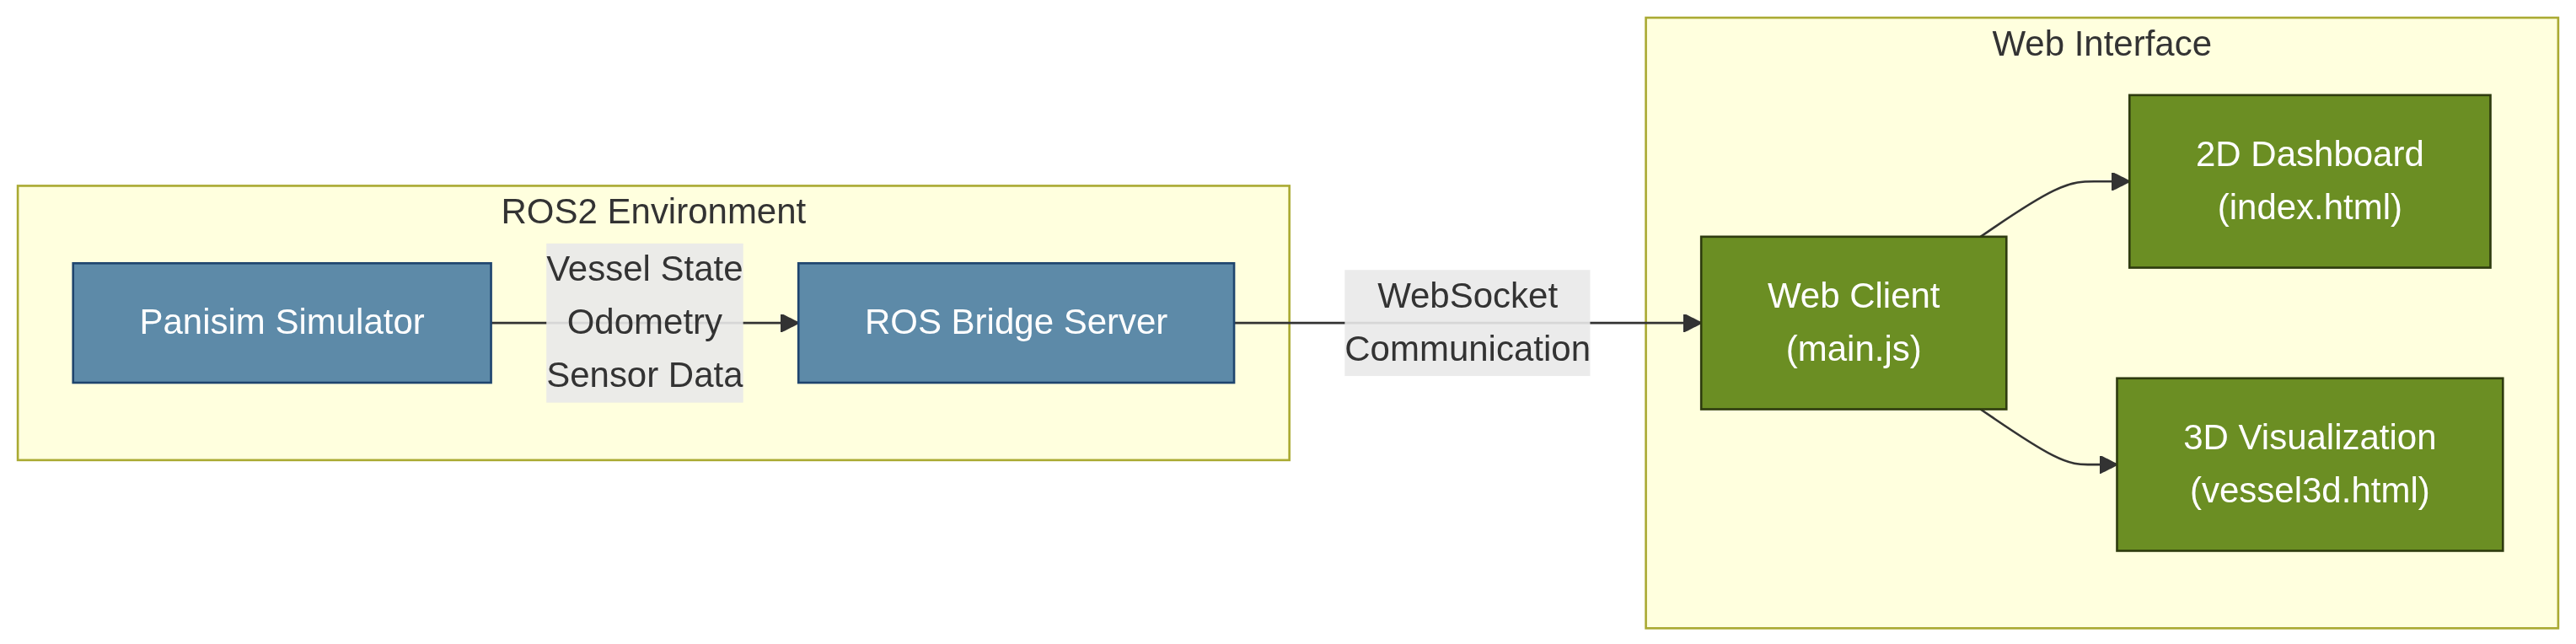
\includegraphics[width=12.13in,height=3.04in]{rawFiles/WebVisualization/web_visualization_files/figure-latex/mermaid-figure-1.png}

\section*{Starting the Visualization}\label{starting-the-visualization}
\addcontentsline{toc}{section}{Starting the Visualization}

\markright{Starting the Visualization}

The web interface is automatically started when launching the Panisim
simulator. It uses:

\begin{enumerate}
\def\labelenumi{\arabic{enumi}.}
\tightlist
\item
  A lightweight HTTP server to host the web files
\item
  The ROS Bridge server for WebSocket communication with ROS2
\end{enumerate}

The visualization launches when running the simulation:

\begin{Shaded}
\begin{Highlighting}[]
\ExtensionTok{ros2}\NormalTok{ launch gnc gnc\_launch.py}
\end{Highlighting}
\end{Shaded}

Once started, you can access the dashboard by opening your web browser:

\begin{itemize}
\tightlist
\item
  \textbf{Main Dashboard}: \texttt{http://localhost:8000/}
\item
  \textbf{3D Visualization}:
  \texttt{http://localhost:8000/vessel3d.html}
\end{itemize}

\section*{Main Dashboard}\label{main-dashboard}
\addcontentsline{toc}{section}{Main Dashboard}

\markright{Main Dashboard}

The main dashboard (index.html) provides a comprehensive overview of the
vessel's state, sensor data, and control inputs.

\subsection*{Key Features}\label{key-features-1}
\addcontentsline{toc}{subsection}{Key Features}

\begin{enumerate}
\def\labelenumi{\arabic{enumi}.}
\tightlist
\item
  \textbf{Vessel Selection}: Switch between different vessels in the
  simulation
\item
  \textbf{Connection Status}: Real-time display of connectivity to the
  ROS2 environment
\item
  \textbf{Vessel Information}: Display of key vessel parameters
  (position, velocity, orientation)
\item
  \textbf{Data Visualizations}: Real-time charts for:

  \begin{itemize}
  \tightlist
  \item
    Vessel path and trajectory
  \item
    Velocities (linear and angular)
  \item
    Orientation (roll, pitch, yaw)
  \item
    Control surface positions
  \item
    Thruster states
  \end{itemize}
\end{enumerate}

\subsection*{Dashboard Layout}\label{dashboard-layout}
\addcontentsline{toc}{subsection}{Dashboard Layout}

The dashboard is organized in a responsive grid layout with cards for
different data categories:

\begin{longtable}[]{@{}
  >{\raggedright\arraybackslash}p{(\linewidth - 2\tabcolsep) * \real{0.4091}}
  >{\raggedright\arraybackslash}p{(\linewidth - 2\tabcolsep) * \real{0.5909}}@{}}
\toprule\noalign{}
\begin{minipage}[b]{\linewidth}\raggedright
Section
\end{minipage} & \begin{minipage}[b]{\linewidth}\raggedright
Description
\end{minipage} \\
\midrule\noalign{}
\endhead
\bottomrule\noalign{}
\endlastfoot
\textbf{Vessel Info} & Basic vessel parameters including position,
velocities, and orientation \\
\textbf{Path Visualization} & 2D trajectory visualization showing vessel
movement in X-Y plane \\
\textbf{Vessel Velocities} & Charts for surge (u), sway (v), and heave
(w) velocities \\
\textbf{Vessel Angular Rates} & Charts for roll rate (p), pitch rate
(q), and yaw rate (r) \\
\textbf{Orientation} & Charts for roll (ϕ), pitch (θ), and yaw (ψ)
angles \\
\textbf{Control Surfaces} & Visual representation of control surface
positions \\
\textbf{Thrusters} & Visual representation of thruster RPMs \\
\end{longtable}

\subsection*{Real-time Data Updates}\label{real-time-data-updates}
\addcontentsline{toc}{subsection}{Real-time Data Updates}

The dashboard updates in real-time with configurable update rates. Data
collection begins automatically when connecting to a vessel and
includes:

\begin{itemize}
\tightlist
\item
  Subscribe to \texttt{/{[}vessel\_name{]}/odometry\_sim} for position
  and velocity data
\item
  Subscribe to \texttt{/{[}vessel\_name{]}/vessel\_state} for complete
  vessel state including actuators
\item
  Optional subscription to additional sensor topics
\end{itemize}

\section*{3D Visualization}\label{d-visualization}
\addcontentsline{toc}{section}{3D Visualization}

\markright{3D Visualization}

The 3D visualization (vessel3d.html) provides an interactive
three-dimensional view of the vessel in its environment.

\subsection*{Key Features}\label{key-features-2}
\addcontentsline{toc}{subsection}{Key Features}

\begin{enumerate}
\def\labelenumi{\arabic{enumi}.}
\tightlist
\item
  \textbf{Real-time Movement}: The vessel model moves and rotates
  according to simulation data
\item
  \textbf{Trajectory Path}: A colored trail showing the vessel's path
  through the environment
\item
  \textbf{Customizable View}: Camera controls for rotating, panning, and
  zooming
\item
  \textbf{Vessel Dimensions}: Adjustable vessel size and proportions to
  match different vessel types
\item
  \textbf{Full-screen Mode}: Expand the visualization to utilize the
  entire screen
\end{enumerate}

\subsection*{Controls}\label{controls}
\addcontentsline{toc}{subsection}{Controls}

The 3D view offers several interactive controls:

\begin{itemize}
\tightlist
\item
  \textbf{Orbit}: Click and drag to rotate the camera around the vessel
\item
  \textbf{Pan}: Right-click and drag (or middle-click and drag) to move
  the camera
\item
  \textbf{Zoom}: Scroll wheel to zoom in and out
\item
  \textbf{Reset Camera}: Button to restore the default camera position
\item
  \textbf{Fullscreen}: Button to toggle fullscreen mode
\end{itemize}

\subsection*{Vessel Model
Customization}\label{vessel-model-customization}
\addcontentsline{toc}{subsection}{Vessel Model Customization}

You can adjust the vessel's appearance through the control panel:

\begin{itemize}
\tightlist
\item
  \textbf{Vessel Size}: Overall scaling of the vessel model
\item
  \textbf{Dimensions}: Individual control over length, width, and height
  proportions
\item
  \textbf{Apply Changes}: Button to update the model with the new
  dimensions
\end{itemize}

\section*{Integration with ROS2}\label{integration-with-ros2}
\addcontentsline{toc}{section}{Integration with ROS2}

\markright{Integration with ROS2}

The visualization dashboard communicates with ROS2 using the ROS Bridge
Server, which provides WebSocket connectivity between the ROS2
environment and web clients.

\subsection*{Communication Flow}\label{communication-flow}
\addcontentsline{toc}{subsection}{Communication Flow}

\begin{enumerate}
\def\labelenumi{\arabic{enumi}.}
\tightlist
\item
  \textbf{ROS2 Topics to WebSockets}: The ROS Bridge Server converts
  ROS2 topic messages to WebSocket messages
\item
  \textbf{Web Client Processing}: JavaScript code processes the
  WebSocket messages and updates the visualizations
\item
  \textbf{Bidirectional Communication}: The system supports both
  subscribing to and publishing ROS2 topics
\end{enumerate}

\subsection*{Required ROS2 Components}\label{required-ros2-components}
\addcontentsline{toc}{subsection}{Required ROS2 Components}

To enable the visualization, the launch file includes:

\begin{Shaded}
\begin{Highlighting}[]
\CommentTok{\# HTTP server for web files}
\NormalTok{ExecuteProcess(}
\NormalTok{    cmd}\OperatorTok{=}\NormalTok{[}\StringTok{\textquotesingle{}python3\textquotesingle{}}\NormalTok{, }\StringTok{\textquotesingle{}{-}m\textquotesingle{}}\NormalTok{, }\StringTok{\textquotesingle{}http.server\textquotesingle{}}\NormalTok{, }\StringTok{\textquotesingle{}8000\textquotesingle{}}\NormalTok{, }\StringTok{\textquotesingle{}{-}{-}directory\textquotesingle{}}\NormalTok{, web\_build\_dir],}
\NormalTok{    name}\OperatorTok{=}\StringTok{\textquotesingle{}http\_server\textquotesingle{}}\NormalTok{,}
\NormalTok{    output}\OperatorTok{=}\StringTok{\textquotesingle{}screen\textquotesingle{}}
\NormalTok{),}

\CommentTok{\# ROS Bridge server for WebSocket communication}
\NormalTok{IncludeLaunchDescription(}
\NormalTok{    AnyLaunchDescriptionSource(rosbridge\_launch)}
\NormalTok{),}
\end{Highlighting}
\end{Shaded}

\subsection*{Topic Subscriptions}\label{topic-subscriptions}
\addcontentsline{toc}{subsection}{Topic Subscriptions}

The visualization automatically discovers vessel topics by querying
available ROS2 topics. It looks for the following patterns:

\begin{itemize}
\tightlist
\item
  \texttt{/\textless{}vessel\_name\textgreater{}/odometry\_sim}: For
  vessel position and velocity
\item
  \texttt{/\textless{}vessel\_name\textgreater{}/vessel\_state}: For
  complete vessel state including actuators
\end{itemize}

\section*{Implementation Details}\label{implementation-details}
\addcontentsline{toc}{section}{Implementation Details}

\markright{Implementation Details}

The visualization dashboard is built using modern web technologies:

\begin{itemize}
\tightlist
\item
  \textbf{Chart.js}: For responsive, interactive data visualization
\item
  \textbf{three.js}: For 3D rendering of the vessel
\item
  \textbf{roslibjs}: For ROS2 communication via WebSockets
\item
  \textbf{Responsive Design}: Automatically adapts to different screen
  sizes
\end{itemize}

\subsection*{Key JavaScript Components}\label{key-javascript-components}
\addcontentsline{toc}{subsection}{Key JavaScript Components}

The system is organized into the following components:

\begin{enumerate}
\def\labelenumi{\arabic{enumi}.}
\tightlist
\item
  \textbf{VesselManager}: Handles vessel discovery, selection, and
  configuration
\item
  \textbf{VesselVisualizer}: Manages data collection, processing, and
  visualization
\item
  \textbf{3D Rendering}: Handles the three-dimensional visualization of
  vessels
\end{enumerate}

\subsection*{Vessel State
Representation}\label{vessel-state-representation}
\addcontentsline{toc}{subsection}{Vessel State Representation}

The dashboard visualizes the complete vessel state model:

\begin{itemize}
\tightlist
\item
  \textbf{Position}: x, y, z (in meters)
\item
  \textbf{Linear Velocity}: u, v, w (in m/s)
\item
  \textbf{Angular Velocity}: p, q, r (in rad/s)
\item
  \textbf{Orientation}: ϕ, θ, ψ (in degrees)
\item
  \textbf{Actuators}: Control surface angles (in degrees) and thruster
  RPMs
\end{itemize}

\section*{Customization Options}\label{customization-options}
\addcontentsline{toc}{section}{Customization Options}

\markright{Customization Options}

The visualization can be customized in several ways:

\begin{enumerate}
\def\labelenumi{\arabic{enumi}.}
\tightlist
\item
  \textbf{Update Rates}: Chart refresh rates can be adjusted
\item
  \textbf{Data Window}: The amount of historical data displayed in
  charts
\item
  \textbf{Vessel Configuration}: The number of control surfaces and
  thrusters displayed
\item
  \textbf{3D Model}: Vessel dimensions and appearance
\item
  \textbf{Chart Scaling}: Auto-rescaling and manual zoom/pan on charts
\end{enumerate}

\section*{Troubleshooting}\label{troubleshooting-1}
\addcontentsline{toc}{section}{Troubleshooting}

\markright{Troubleshooting}

\subsection*{Connection Issues}\label{connection-issues}
\addcontentsline{toc}{subsection}{Connection Issues}

If the dashboard shows ``Disconnected'' status:

\begin{enumerate}
\def\labelenumi{\arabic{enumi}.}
\tightlist
\item
  Ensure the ROS Bridge server is running
\item
  Check that WebSocket port 9090 is accessible
\item
  Verify the simulator is publishing required topics
\end{enumerate}

\subsection*{Missing Vessel Data}\label{missing-vessel-data}
\addcontentsline{toc}{subsection}{Missing Vessel Data}

If vessel data isn't displaying:

\begin{enumerate}
\def\labelenumi{\arabic{enumi}.}
\item
  Select a vessel from the dropdown menu
\item
  Check ROS2 topics are being published:

\begin{Shaded}
\begin{Highlighting}[]
\ExtensionTok{ros2}\NormalTok{ topic list }\KeywordTok{|} \FunctionTok{grep}\NormalTok{ vessel}
\end{Highlighting}
\end{Shaded}
\item
  Verify message publication with:

\begin{Shaded}
\begin{Highlighting}[]
\ExtensionTok{ros2}\NormalTok{ topic echo /}\OperatorTok{\textless{}}\NormalTok{vessel\_name}\OperatorTok{\textgreater{}}\NormalTok{/odometry\_sim}
\end{Highlighting}
\end{Shaded}
\end{enumerate}

\subsection*{Browser Compatibility}\label{browser-compatibility}
\addcontentsline{toc}{subsection}{Browser Compatibility}

The visualization works best with modern browsers:

\begin{itemize}
\tightlist
\item
  Google Chrome
\item
  Mozilla Firefox\\
\item
  Microsoft Edge
\item
  Brave Browser
\end{itemize}

\section*{Conclusion}\label{conclusion}
\addcontentsline{toc}{section}{Conclusion}

\markright{Conclusion}

The Panisim visualization dashboard provides a comprehensive interface
for monitoring and interacting with simulated vessels. With its
real-time updates, interactive charts, and 3D visualization, it offers a
powerful tool for understanding vessel behavior and validating custom
control or guidance algorithms.

\bookmarksetup{startatroot}

\chapter*{Example - Creating a ROS2 Waypoint Tracking
Controller}\label{example---creating-a-ros2-waypoint-tracking-controller}
\addcontentsline{toc}{chapter}{Example - Creating a ROS2 Waypoint
Tracking Controller}

\markboth{Example - Creating a ROS2 Waypoint Tracking
Controller}{Example - Creating a ROS2 Waypoint Tracking Controller}

\section*{Overview}\label{overview-8}
\addcontentsline{toc}{section}{Overview}

\markright{Overview}

This example demonstrates how to create a custom ROS2 package to
interact with the Panisim simulator. We'll build a Guidance, Navigation,
and Control (GNC) package that implements a waypoint tracking PID
controller for marine vessels. This example covers:

\begin{enumerate}
\def\labelenumi{\arabic{enumi}.}
\tightlist
\item
  Creating a ROS2 package structure
\item
  Implementing core controller logic
\item
  Setting up ROS2 nodes to interface with the simulator
\item
  Building and launching the complete system
\end{enumerate}

\begin{tcolorbox}[enhanced jigsaw, colback=white, toptitle=1mm, colframe=quarto-callout-tip-color-frame, rightrule=.15mm, breakable, title=\textcolor{quarto-callout-tip-color}{\faLightbulb}\hspace{0.5em}{Tip}, toprule=.15mm, opacitybacktitle=0.6, opacityback=0, coltitle=black, leftrule=.75mm, colbacktitle=quarto-callout-tip-color!10!white, arc=.35mm, titlerule=0mm, bottomtitle=1mm, bottomrule=.15mm, left=2mm]

All the below codes and folders are already implemented in the
Repository. This example is only for the reference and to show how you
can configure your own ROS2 package to interact with the Panisim
simulator.

\end{tcolorbox}

\section*{Creating the ROS2 Package}\label{creating-the-ros2-package}
\addcontentsline{toc}{section}{Creating the ROS2 Package}

\markright{Creating the ROS2 Package}

\subsection*{1. Package Structure}\label{package-structure}
\addcontentsline{toc}{subsection}{1. Package Structure}

First, let's create a new ROS2 package called \texttt{gnc} in the
\texttt{ros2\_ws/src} directory:

\begin{Shaded}
\begin{Highlighting}[]
\BuiltInTok{cd}\NormalTok{ ros2\_ws/src}
\ExtensionTok{ros2}\NormalTok{ pkg create }\AttributeTok{{-}{-}build{-}type}\NormalTok{ ament\_python gnc }\AttributeTok{{-}{-}dependencies}\NormalTok{ rclpy nav\_msgs geometry\_msgs interfaces}
\end{Highlighting}
\end{Shaded}

This creates a basic package structure:

\begin{verbatim}
gnc/
├── gnc/
│   └── __init__.py
├── package.xml
├── setup.py
└── setup.cfg
\end{verbatim}

\subsection*{2. Update Package
Dependencies}\label{update-package-dependencies}
\addcontentsline{toc}{subsection}{2. Update Package Dependencies}

Edit \texttt{package.xml} to include all required dependencies:

\begin{Shaded}
\begin{Highlighting}[]
\FunctionTok{\textless{}?xml}\OtherTok{ version=}\StringTok{"1.0"}\FunctionTok{?\textgreater{}}
\FunctionTok{\textless{}?xml{-}model}\NormalTok{ href="http://download.ros.org/schema/package\_format3.xsd" schematypens="http://www.w3.org/2001/XMLSchema"}\FunctionTok{?\textgreater{}}
\NormalTok{\textless{}}\KeywordTok{package}\OtherTok{ format=}\StringTok{"3"}\NormalTok{\textgreater{}}
\NormalTok{  \textless{}}\KeywordTok{name}\NormalTok{\textgreater{}gnc\textless{}/}\KeywordTok{name}\NormalTok{\textgreater{}}
\NormalTok{  \textless{}}\KeywordTok{version}\NormalTok{\textgreater{}0.0.1\textless{}/}\KeywordTok{version}\NormalTok{\textgreater{}}
\NormalTok{  \textless{}}\KeywordTok{description}\NormalTok{\textgreater{}Guidance, Navigation and Control package for Panisim\textless{}/}\KeywordTok{description}\NormalTok{\textgreater{}}
\NormalTok{  \textless{}}\KeywordTok{maintainer}\OtherTok{ email=}\StringTok{"example@example.com"}\NormalTok{\textgreater{}user\textless{}/}\KeywordTok{maintainer}\NormalTok{\textgreater{}}
\NormalTok{  \textless{}}\KeywordTok{license}\NormalTok{\textgreater{}Apache License 2.0\textless{}/}\KeywordTok{license}\NormalTok{\textgreater{}}

\NormalTok{  \textless{}}\KeywordTok{depend}\NormalTok{\textgreater{}rclpy\textless{}/}\KeywordTok{depend}\NormalTok{\textgreater{}}
\NormalTok{  \textless{}}\KeywordTok{depend}\NormalTok{\textgreater{}nav\_msgs\textless{}/}\KeywordTok{depend}\NormalTok{\textgreater{}}
\NormalTok{  \textless{}}\KeywordTok{depend}\NormalTok{\textgreater{}geometry\_msgs\textless{}/}\KeywordTok{depend}\NormalTok{\textgreater{}}
\NormalTok{  \textless{}}\KeywordTok{depend}\NormalTok{\textgreater{}std\_msgs\textless{}/}\KeywordTok{depend}\NormalTok{\textgreater{}}
\NormalTok{  \textless{}}\KeywordTok{depend}\NormalTok{\textgreater{}interfaces\textless{}/}\KeywordTok{depend}\NormalTok{\textgreater{}}
\NormalTok{  \textless{}}\KeywordTok{depend}\NormalTok{\textgreater{}mav\_simulator\textless{}/}\KeywordTok{depend}\NormalTok{\textgreater{}}
  
\NormalTok{  \textless{}}\KeywordTok{exec\_depend}\NormalTok{\textgreater{}ros2launch\textless{}/}\KeywordTok{exec\_depend}\NormalTok{\textgreater{}}

\NormalTok{  \textless{}}\KeywordTok{export}\NormalTok{\textgreater{}}
\NormalTok{    \textless{}}\KeywordTok{build\_type}\NormalTok{\textgreater{}ament\_python\textless{}/}\KeywordTok{build\_type}\NormalTok{\textgreater{}}
\NormalTok{  \textless{}/}\KeywordTok{export}\NormalTok{\textgreater{}}
\NormalTok{\textless{}/}\KeywordTok{package}\NormalTok{\textgreater{}}
\end{Highlighting}
\end{Shaded}

\subsection*{3. Configure Setup Scripts}\label{configure-setup-scripts}
\addcontentsline{toc}{subsection}{3. Configure Setup Scripts}

Update \texttt{setup.py} to include our entry points and specify
dependencies:

\begin{Shaded}
\begin{Highlighting}[]
\ImportTok{from}\NormalTok{ setuptools }\ImportTok{import}\NormalTok{ setup}
\ImportTok{import}\NormalTok{ os}
\ImportTok{from}\NormalTok{ glob }\ImportTok{import}\NormalTok{ glob}

\NormalTok{package\_name }\OperatorTok{=} \StringTok{\textquotesingle{}gnc\textquotesingle{}}

\NormalTok{setup(}
\NormalTok{    name}\OperatorTok{=}\NormalTok{package\_name,}
\NormalTok{    version}\OperatorTok{=}\StringTok{\textquotesingle{}0.0.1\textquotesingle{}}\NormalTok{,}
\NormalTok{    packages}\OperatorTok{=}\NormalTok{[package\_name],}
\NormalTok{    data\_files}\OperatorTok{=}\NormalTok{[}
\NormalTok{        (}\StringTok{\textquotesingle{}share/ament\_index/resource\_index/packages\textquotesingle{}}\NormalTok{,}
\NormalTok{            [}\StringTok{\textquotesingle{}resource/\textquotesingle{}} \OperatorTok{+}\NormalTok{ package\_name]),}
\NormalTok{        (}\StringTok{\textquotesingle{}share/\textquotesingle{}} \OperatorTok{+}\NormalTok{ package\_name, [}\StringTok{\textquotesingle{}package.xml\textquotesingle{}}\NormalTok{]),}
\NormalTok{        (os.path.join(}\StringTok{\textquotesingle{}share\textquotesingle{}}\NormalTok{, package\_name, }\StringTok{\textquotesingle{}launch\textquotesingle{}}\NormalTok{), glob(}\StringTok{\textquotesingle{}launch/*.py\textquotesingle{}}\NormalTok{)),}
\NormalTok{        (os.path.join(}\StringTok{\textquotesingle{}share\textquotesingle{}}\NormalTok{, package\_name, }\StringTok{\textquotesingle{}web\textquotesingle{}}\NormalTok{), glob(}\StringTok{\textquotesingle{}web/**/*\textquotesingle{}}\NormalTok{, recursive}\OperatorTok{=}\VariableTok{True}\NormalTok{)),}
\NormalTok{    ],}
\NormalTok{    install\_requires}\OperatorTok{=}\NormalTok{[}\StringTok{\textquotesingle{}setuptools\textquotesingle{}}\NormalTok{],}
\NormalTok{    zip\_safe}\OperatorTok{=}\VariableTok{True}\NormalTok{,}
\NormalTok{    maintainer}\OperatorTok{=}\StringTok{\textquotesingle{}user\textquotesingle{}}\NormalTok{,}
\NormalTok{    maintainer\_email}\OperatorTok{=}\StringTok{\textquotesingle{}example@example.com\textquotesingle{}}\NormalTok{,}
\NormalTok{    description}\OperatorTok{=}\StringTok{\textquotesingle{}Guidance, Navigation and Control package for Panisim\textquotesingle{}}\NormalTok{,}
\NormalTok{    license}\OperatorTok{=}\StringTok{\textquotesingle{}Apache License 2.0\textquotesingle{}}\NormalTok{,}
\NormalTok{    tests\_require}\OperatorTok{=}\NormalTok{[}\StringTok{\textquotesingle{}pytest\textquotesingle{}}\NormalTok{],}
\NormalTok{    entry\_points}\OperatorTok{=}\NormalTok{\{}
        \StringTok{\textquotesingle{}console\_scripts\textquotesingle{}}\NormalTok{: [}
            \StringTok{\textquotesingle{}gc = gnc.guidance\_control:main\textquotesingle{}}\NormalTok{,}
            \StringTok{\textquotesingle{}nav = gnc.navigation:main\textquotesingle{}}\NormalTok{,}
\NormalTok{        ],}
\NormalTok{    \},}
\NormalTok{)}
\end{Highlighting}
\end{Shaded}

\subsection*{4. Create Directory
Structure}\label{create-directory-structure}
\addcontentsline{toc}{subsection}{4. Create Directory Structure}

Set up the complete directory structure:

\begin{Shaded}
\begin{Highlighting}[]
\FunctionTok{mkdir} \AttributeTok{{-}p}\NormalTok{ gnc/launch}
\FunctionTok{mkdir} \AttributeTok{{-}p}\NormalTok{ gnc/web}
\end{Highlighting}
\end{Shaded}

\section*{Implementing the Controller
Logic}\label{implementing-the-controller-logic}
\addcontentsline{toc}{section}{Implementing the Controller Logic}

\markright{Implementing the Controller Logic}

\subsection*{1. Control Module}\label{control-module}
\addcontentsline{toc}{subsection}{1. Control Module}

First, create \texttt{module\_control.py} in the gnc package to
implement the PID control logic:

\begin{Shaded}
\begin{Highlighting}[]
\CommentTok{\# ros2\_ws/src/gnc/gnc/module\_control.py}
\ImportTok{import}\NormalTok{ numpy }\ImportTok{as}\NormalTok{ np}

\CommentTok{"""}
\CommentTok{Rudder control module for vessel simulation.}

\CommentTok{This module provides rudder control strategies for vessel steering with PID controllers.}
\CommentTok{"""}

\KeywordTok{def}\NormalTok{ ssa(ang, deg}\OperatorTok{=}\VariableTok{False}\NormalTok{):}
    \CommentTok{"""}
\CommentTok{    Smallest signed angle that lies between {-}pi and pi.}
\CommentTok{    If deg is True, the angle is assumed to be in degrees and is converted to radians.}
\CommentTok{    If deg is False, the angle is assumed to be in radians.}
\CommentTok{    """}
    \ControlFlowTok{if}\NormalTok{ deg:}
\NormalTok{        ang }\OperatorTok{=}\NormalTok{ (ang }\OperatorTok{+} \DecValTok{180}\NormalTok{) }\OperatorTok{\%}\NormalTok{ (}\FloatTok{360.0}\NormalTok{) }\OperatorTok{{-}} \FloatTok{180.0}
    \ControlFlowTok{else}\NormalTok{:}
\NormalTok{        ang }\OperatorTok{=}\NormalTok{ (ang }\OperatorTok{+}\NormalTok{ np.pi) }\OperatorTok{\%}\NormalTok{ (}\DecValTok{2} \OperatorTok{*}\NormalTok{ np.pi) }\OperatorTok{{-}}\NormalTok{ np.pi}
    \ControlFlowTok{return}\NormalTok{ ang}

\KeywordTok{def}\NormalTok{ clip(val, min\_val, max\_val):}
    \CommentTok{"""}
\CommentTok{    Clip a value to a range.}
\CommentTok{    """}
    \ControlFlowTok{return} \BuiltInTok{max}\NormalTok{(min\_val, }\BuiltInTok{min}\NormalTok{(val, max\_val))}

\KeywordTok{def}\NormalTok{ pid\_control(t, state, waypoints, waypoint\_idx, ye\_int}\OperatorTok{=}\FloatTok{0.0}\NormalTok{):}
    \CommentTok{"""}
\CommentTok{    Implement a PID control strategy to follow the waypoints. }
\CommentTok{    }
\CommentTok{    Args:}
\CommentTok{        t (float): Current simulation time [s]}
\CommentTok{        state (ndarray): Current vessel state vector}
\CommentTok{        waypoints (ndarray): Waypoints array}
\CommentTok{        waypoint\_idx (int): Current waypoint index}
\CommentTok{        ye\_int (float): Integral term of cross{-}track error}
\CommentTok{        }
\CommentTok{    Returns:}
\CommentTok{        float: Commanded rudder angle in radians}
\CommentTok{        float: Cross{-}track error}
\CommentTok{        int: Next waypoint index}
\CommentTok{    """}

    \CommentTok{\# Check if we have reached the last waypoint}
    \ControlFlowTok{if}\NormalTok{ waypoint\_idx }\OperatorTok{==} \BuiltInTok{len}\NormalTok{(waypoints):}
        \ControlFlowTok{return} \FloatTok{0.0}\NormalTok{, }\FloatTok{0.0}\NormalTok{, waypoint\_idx}

    \CommentTok{\# Current state}
\NormalTok{    u, v, r }\OperatorTok{=}\NormalTok{ state[}\DecValTok{3}\NormalTok{], state[}\DecValTok{4}\NormalTok{], state[}\DecValTok{5}\NormalTok{]}
\NormalTok{    x, y, psi }\OperatorTok{=}\NormalTok{ state[}\DecValTok{6}\NormalTok{], state[}\DecValTok{7}\NormalTok{], state[}\DecValTok{11}\NormalTok{]}
    
    \CommentTok{\# Current and previous waypoints}
\NormalTok{    wp\_xn, wp\_yn, \_ }\OperatorTok{=}\NormalTok{ waypoints[waypoint\_idx]}
\NormalTok{    wp\_xn1, wp\_yn1, \_ }\OperatorTok{=}\NormalTok{ waypoints[waypoint\_idx }\OperatorTok{{-}} \DecValTok{1}\NormalTok{]}

    \CommentTok{\# Calculate path line equation: ax + by + c = 0}
\NormalTok{    a }\OperatorTok{=} \OperatorTok{{-}}\NormalTok{(wp\_yn1 }\OperatorTok{{-}}\NormalTok{ wp\_yn)}
\NormalTok{    b }\OperatorTok{=}\NormalTok{ (wp\_xn1 }\OperatorTok{{-}}\NormalTok{ wp\_xn)}
\NormalTok{    c }\OperatorTok{=} \OperatorTok{{-}}\NormalTok{wp\_yn1}\OperatorTok{*}\NormalTok{b}\OperatorTok{{-}}\NormalTok{a}\OperatorTok{*}\NormalTok{wp\_xn1}
    
    \CommentTok{\# Path direction unit vector}
\NormalTok{    wp\_unit\_vec }\OperatorTok{=}\NormalTok{ np.array([wp\_xn }\OperatorTok{{-}}\NormalTok{ wp\_xn1, wp\_yn }\OperatorTok{{-}}\NormalTok{ wp\_yn1, }\FloatTok{0.0}\NormalTok{])}
\NormalTok{    wp\_unit\_vec }\OperatorTok{=}\NormalTok{ wp\_unit\_vec }\OperatorTok{/}\NormalTok{ np.linalg.norm(wp\_unit\_vec)}

    \CommentTok{\# Calculate cross{-}track error}
\NormalTok{    ye }\OperatorTok{=} \OperatorTok{{-}}\NormalTok{(a}\OperatorTok{*}\NormalTok{x }\OperatorTok{+}\NormalTok{ b}\OperatorTok{*}\NormalTok{y }\OperatorTok{+}\NormalTok{ c)}\OperatorTok{/}\NormalTok{np.sqrt(a}\OperatorTok{**}\DecValTok{2} \OperatorTok{+}\NormalTok{ b}\OperatorTok{**}\DecValTok{2}\NormalTok{)}
    
    \CommentTok{\# Path direction angle}
\NormalTok{    pi\_p }\OperatorTok{=}\NormalTok{ np.angle(wp\_unit\_vec[}\DecValTok{0}\NormalTok{] }\OperatorTok{+} \OtherTok{1j} \OperatorTok{*}\NormalTok{ wp\_unit\_vec[}\DecValTok{1}\NormalTok{]) }

    \CommentTok{\# Outer loop PID gains}
\NormalTok{    Kpo }\OperatorTok{=} \FloatTok{0.6}  \CommentTok{\# Proportional gain}
\NormalTok{    Kio }\OperatorTok{=} \FloatTok{0.05} \CommentTok{\# Integral gain}
    
    \CommentTok{\# Desired heading (outer loop control)}
\NormalTok{    psid }\OperatorTok{=}\NormalTok{ pi\_p }\OperatorTok{+}\NormalTok{ Kpo}\OperatorTok{*}\NormalTok{(}\OperatorTok{{-}}\NormalTok{ye) }\OperatorTok{+}\NormalTok{ Kio}\OperatorTok{*}\NormalTok{(}\OperatorTok{{-}}\NormalTok{ye\_int)}
   
    \CommentTok{\# Inner loop PID gains}
\NormalTok{    Kpi }\OperatorTok{=} \FloatTok{0.7}  \CommentTok{\# Proportional gain}
\NormalTok{    Kdi }\OperatorTok{=} \FloatTok{0.5}  \CommentTok{\# Derivative gain}
    
    \CommentTok{\# Rudder command (inner loop control)}
\NormalTok{    delta\_c }\OperatorTok{=}\NormalTok{ Kpi}\OperatorTok{*}\NormalTok{ssa(psid }\OperatorTok{{-}}\NormalTok{ psi) }\OperatorTok{+}\NormalTok{ Kdi}\OperatorTok{*}\NormalTok{(}\DecValTok{0} \OperatorTok{{-}}\NormalTok{ r)}
    
    \CommentTok{\# Clip the rudder angle}
\NormalTok{    delta\_c }\OperatorTok{=}\NormalTok{ clip(delta\_c, }\OperatorTok{{-}}\DecValTok{35}\OperatorTok{*}\NormalTok{np.pi}\OperatorTok{/}\DecValTok{180}\NormalTok{, }\DecValTok{35}\OperatorTok{*}\NormalTok{np.pi}\OperatorTok{/}\DecValTok{180}\NormalTok{)}

    \CommentTok{\# Distance to waypoint}
\NormalTok{    wp\_dist }\OperatorTok{=}\NormalTok{ np.linalg.norm(np.array([x }\OperatorTok{{-}}\NormalTok{ wp\_xn, y }\OperatorTok{{-}}\NormalTok{ wp\_yn, }\FloatTok{0.0}\NormalTok{]))}
    \ControlFlowTok{if}\NormalTok{ wp\_dist }\OperatorTok{\textless{}} \FloatTok{0.5}\NormalTok{:  }\CommentTok{\# 0.5m threshold}
\NormalTok{        waypoint\_idx }\OperatorTok{+=} \DecValTok{1}

    \CommentTok{\# Return negative delta\_c (due to sign convention of rudder angle)}
    \ControlFlowTok{return} \OperatorTok{{-}}\NormalTok{delta\_c, ye, waypoint\_idx}
\end{Highlighting}
\end{Shaded}

\subsection*{2. Guidance Control Node
Class}\label{guidance-control-node-class}
\addcontentsline{toc}{subsection}{2. Guidance Control Node Class}

Next, create \texttt{class\_guidance\_control.py} to implement the ROS2
node class:

\begin{Shaded}
\begin{Highlighting}[]
\CommentTok{\# ros2\_ws/src/gnc/gnc/class\_guidance\_control.py}
\ImportTok{from}\NormalTok{ rclpy.node }\ImportTok{import}\NormalTok{ Node}
\ImportTok{from}\NormalTok{ nav\_msgs.msg }\ImportTok{import}\NormalTok{ Odometry}
\ImportTok{from}\NormalTok{ interfaces.msg }\ImportTok{import}\NormalTok{ Actuator}
\ImportTok{from}\NormalTok{ geometry\_msgs.msg }\ImportTok{import}\NormalTok{ PoseArray, Pose}
\ImportTok{from}\NormalTok{ mav\_simulator.module\_kinematics }\ImportTok{import}\NormalTok{ quat\_to\_eul}
\ImportTok{import}\NormalTok{ gnc.module\_control }\ImportTok{as}\NormalTok{ con}
\ImportTok{import}\NormalTok{ numpy }\ImportTok{as}\NormalTok{ np}

\KeywordTok{class}\NormalTok{ GuidanceControl(Node):}
    \KeywordTok{def} \FunctionTok{\_\_init\_\_}\NormalTok{(}\VariableTok{self}\NormalTok{, vessel):}
        \BuiltInTok{super}\NormalTok{().}\FunctionTok{\_\_init\_\_}\NormalTok{(}\StringTok{\textquotesingle{}guidance\_controller\textquotesingle{}}\NormalTok{)}

        \VariableTok{self}\NormalTok{.vessel }\OperatorTok{=}\NormalTok{ vessel}
        
        \CommentTok{\# Configure topics based on vessel name and ID}
        \VariableTok{self}\NormalTok{.odom\_topic }\OperatorTok{=} \SpecialStringTok{f\textquotesingle{}}\SpecialCharTok{\{}\VariableTok{self}\SpecialCharTok{.}\NormalTok{vessel}\SpecialCharTok{.}\NormalTok{vessel\_name}\SpecialCharTok{\}}\SpecialStringTok{\_}\SpecialCharTok{\{}\VariableTok{self}\SpecialCharTok{.}\NormalTok{vessel}\SpecialCharTok{.}\NormalTok{vessel\_id}\SpecialCharTok{:02d\}}\SpecialStringTok{/odometry\_sim\textquotesingle{}}
        \VariableTok{self}\NormalTok{.actuator\_topic }\OperatorTok{=} \SpecialStringTok{f\textquotesingle{}}\SpecialCharTok{\{}\VariableTok{self}\SpecialCharTok{.}\NormalTok{vessel}\SpecialCharTok{.}\NormalTok{vessel\_name}\SpecialCharTok{\}}\SpecialStringTok{\_}\SpecialCharTok{\{}\VariableTok{self}\SpecialCharTok{.}\NormalTok{vessel}\SpecialCharTok{.}\NormalTok{vessel\_id}\SpecialCharTok{:02d\}}\SpecialStringTok{/actuator\_cmd\textquotesingle{}}
        \VariableTok{self}\NormalTok{.waypoints\_topic }\OperatorTok{=} \SpecialStringTok{f\textquotesingle{}}\SpecialCharTok{\{}\VariableTok{self}\SpecialCharTok{.}\NormalTok{vessel}\SpecialCharTok{.}\NormalTok{vessel\_name}\SpecialCharTok{\}}\SpecialStringTok{\_}\SpecialCharTok{\{}\VariableTok{self}\SpecialCharTok{.}\NormalTok{vessel}\SpecialCharTok{.}\NormalTok{vessel\_id}\SpecialCharTok{:02d\}}\SpecialStringTok{/waypoints\textquotesingle{}}
        
        \CommentTok{\# Create subscriber for odometry}
        \VariableTok{self}\NormalTok{.odom\_sub }\OperatorTok{=} \VariableTok{self}\NormalTok{.create\_subscription(}
\NormalTok{            Odometry,}
            \VariableTok{self}\NormalTok{.odom\_topic,}
            \VariableTok{self}\NormalTok{.odom\_callback,}
            \DecValTok{10}\NormalTok{)}
            
        \CommentTok{\# Create publisher for rudder command}
        \VariableTok{self}\NormalTok{.actuator\_pub }\OperatorTok{=} \VariableTok{self}\NormalTok{.create\_publisher(}
\NormalTok{            Actuator,}
            \VariableTok{self}\NormalTok{.actuator\_topic,}
            \DecValTok{10}\NormalTok{)}
        
        \CommentTok{\# Create publisher for waypoints}
        \VariableTok{self}\NormalTok{.waypoints\_pub }\OperatorTok{=} \VariableTok{self}\NormalTok{.create\_publisher(}
\NormalTok{            PoseArray,}
            \VariableTok{self}\NormalTok{.waypoints\_topic,}
            \DecValTok{10}\NormalTok{)}
        
        \CommentTok{\# Set up timer to publish waypoints}
        \VariableTok{self}\NormalTok{.timer }\OperatorTok{=} \VariableTok{self}\NormalTok{.create\_timer(}\FloatTok{1.0}\NormalTok{, }\VariableTok{self}\NormalTok{.publish\_waypoints)}
        
        \CommentTok{\# Read waypoints from vessel configuration}
        \VariableTok{self}\NormalTok{.waypoints }\OperatorTok{=}\NormalTok{ np.array(}\VariableTok{self}\NormalTok{.vessel.vessel\_config[}\StringTok{\textquotesingle{}guidance\textquotesingle{}}\NormalTok{][}\StringTok{\textquotesingle{}waypoints\textquotesingle{}}\NormalTok{])}
        \VariableTok{self}\NormalTok{.waypoints\_type }\OperatorTok{=} \VariableTok{self}\NormalTok{.vessel.vessel\_config[}\StringTok{\textquotesingle{}guidance\textquotesingle{}}\NormalTok{][}\StringTok{\textquotesingle{}waypoints\_type\textquotesingle{}}\NormalTok{]}
        \VariableTok{self}\NormalTok{.waypoint\_idx }\OperatorTok{=} \DecValTok{1}

        \VariableTok{self}\NormalTok{.waypoints\_data }\OperatorTok{=}\NormalTok{ \{}
            \StringTok{\textquotesingle{}waypoints\textquotesingle{}}\NormalTok{: }\VariableTok{self}\NormalTok{.waypoints,}
            \StringTok{\textquotesingle{}waypoints\_type\textquotesingle{}}\NormalTok{: }\VariableTok{self}\NormalTok{.waypoints\_type}
\NormalTok{        \}}
        
        \CommentTok{\# Initialize time}
        \VariableTok{self}\NormalTok{.start\_time }\OperatorTok{=} \VariableTok{self}\NormalTok{.get\_clock().now()}

        \CommentTok{\# Initialize integrator}
        \VariableTok{self}\NormalTok{.ye\_int }\OperatorTok{=} \FloatTok{0.0}
        \VariableTok{self}\NormalTok{.te\_int }\OperatorTok{=} \FloatTok{0.0}
        
        \CommentTok{\# Select control mode}
        \VariableTok{self}\NormalTok{.control\_mode }\OperatorTok{=}\NormalTok{ con.pid\_control}
        
        \VariableTok{self}\NormalTok{.get\_logger().info(}\StringTok{\textquotesingle{}Guidance Controller initialized\textquotesingle{}}\NormalTok{)}

    \KeywordTok{def}\NormalTok{ publish\_waypoints(}\VariableTok{self}\NormalTok{):}
        \CommentTok{"""Publish waypoints for visualization"""}
        \ControlFlowTok{if} \KeywordTok{not} \VariableTok{self}\NormalTok{.waypoints\_data:}
            \ControlFlowTok{return}
            
\NormalTok{        pose\_array }\OperatorTok{=}\NormalTok{ PoseArray()}
\NormalTok{        pose\_array.header.stamp }\OperatorTok{=} \VariableTok{self}\NormalTok{.get\_clock().now().to\_msg()}
\NormalTok{        pose\_array.header.frame\_id }\OperatorTok{=} \StringTok{"map"}
        
        \ControlFlowTok{for}\NormalTok{ waypoint }\KeywordTok{in} \VariableTok{self}\NormalTok{.waypoints\_data.get(}\StringTok{\textquotesingle{}waypoints\textquotesingle{}}\NormalTok{, []):}
\NormalTok{            pose }\OperatorTok{=}\NormalTok{ Pose()}
\NormalTok{            pose.position.x }\OperatorTok{=} \BuiltInTok{float}\NormalTok{(waypoint[}\DecValTok{0}\NormalTok{])}
\NormalTok{            pose.position.y }\OperatorTok{=} \BuiltInTok{float}\NormalTok{(waypoint[}\DecValTok{1}\NormalTok{])}
\NormalTok{            pose.position.z }\OperatorTok{=} \BuiltInTok{float}\NormalTok{(waypoint[}\DecValTok{2}\NormalTok{])}
\NormalTok{            pose\_array.poses.append(pose)}
        
        \VariableTok{self}\NormalTok{.waypoints\_pub.publish(pose\_array)}
    
    \KeywordTok{def}\NormalTok{ odom\_callback(}\VariableTok{self}\NormalTok{, msg):}
        \CommentTok{"""Process odometry data and calculate control commands"""}
        \CommentTok{\# Get current time in seconds}
\NormalTok{        current\_time }\OperatorTok{=} \VariableTok{self}\NormalTok{.get\_clock().now()}
\NormalTok{        t }\OperatorTok{=}\NormalTok{ (current\_time }\OperatorTok{{-}} \VariableTok{self}\NormalTok{.start\_time).nanoseconds }\OperatorTok{/} \FloatTok{1e9}

        \CommentTok{\# Extract orientation quaternion}
\NormalTok{        quat }\OperatorTok{=}\NormalTok{ np.array([}
\NormalTok{            msg.pose.pose.orientation.w,}
\NormalTok{            msg.pose.pose.orientation.x,}
\NormalTok{            msg.pose.pose.orientation.y,}
\NormalTok{            msg.pose.pose.orientation.z}
\NormalTok{        ])}

        \CommentTok{\# Convert quaternion to Euler angles}
\NormalTok{        eul }\OperatorTok{=}\NormalTok{ quat\_to\_eul(quat, order}\OperatorTok{=}\StringTok{\textquotesingle{}ZYX\textquotesingle{}}\NormalTok{)}
        
        \CommentTok{\# Create state vector from odometry}
\NormalTok{        state }\OperatorTok{=}\NormalTok{ np.array([            }
\NormalTok{            msg.twist.twist.linear.x,}
\NormalTok{            msg.twist.twist.linear.y,}
\NormalTok{            msg.twist.twist.linear.z,}
\NormalTok{            msg.twist.twist.angular.x,}
\NormalTok{            msg.twist.twist.angular.y,}
\NormalTok{            msg.twist.twist.angular.z,}
\NormalTok{            msg.pose.pose.position.x,}
\NormalTok{            msg.pose.pose.position.y,}
\NormalTok{            msg.pose.pose.position.z,}
\NormalTok{            eul[}\DecValTok{0}\NormalTok{],}
\NormalTok{            eul[}\DecValTok{1}\NormalTok{],}
\NormalTok{            eul[}\DecValTok{2}\NormalTok{],}
            \FloatTok{0.0} \CommentTok{\# rudder angle}
\NormalTok{        ])}

        \CommentTok{\# Calculate control command}
\NormalTok{        rudder\_cmd, ye, wp\_indx }\OperatorTok{=} \VariableTok{self}\NormalTok{.control\_mode(t, state, }\VariableTok{self}\NormalTok{.waypoints, }\VariableTok{self}\NormalTok{.waypoint\_idx, }\VariableTok{self}\NormalTok{.ye\_int)}

        \CommentTok{\# Handle waypoint transitions}
        \ControlFlowTok{if}\NormalTok{ wp\_indx }\OperatorTok{!=} \VariableTok{self}\NormalTok{.waypoint\_idx:}
            \VariableTok{self}\NormalTok{.get\_logger().info(}\SpecialStringTok{f\textquotesingle{}Waypoint }\SpecialCharTok{\{}\VariableTok{self}\SpecialCharTok{.}\NormalTok{waypoint\_idx}\SpecialCharTok{\}}\SpecialStringTok{ reached\textquotesingle{}}\NormalTok{)}
            \VariableTok{self}\NormalTok{.waypoint\_idx }\OperatorTok{=}\NormalTok{ wp\_indx}
            \VariableTok{self}\NormalTok{.ye\_int }\OperatorTok{=} \FloatTok{0.0}  \CommentTok{\# Reset integral term}

            \CommentTok{\# Loop back to first waypoint when all are visited}
            \ControlFlowTok{if} \VariableTok{self}\NormalTok{.waypoint\_idx }\OperatorTok{\textgreater{}=} \BuiltInTok{len}\NormalTok{(}\VariableTok{self}\NormalTok{.waypoints):}
                \VariableTok{self}\NormalTok{.get\_logger().info(}\StringTok{\textquotesingle{}***All waypoints reached***\textquotesingle{}}\NormalTok{)}
                \VariableTok{self}\NormalTok{.waypoint\_idx }\OperatorTok{=} \DecValTok{1}

        \CommentTok{\# Calculate time difference for integration}
\NormalTok{        dt }\OperatorTok{=}\NormalTok{ t }\OperatorTok{{-}} \VariableTok{self}\NormalTok{.te\_int}
        \ControlFlowTok{if}\NormalTok{ dt }\OperatorTok{\textgreater{}} \DecValTok{0}\NormalTok{:  }\CommentTok{\# Avoid division by zero or negative time}
            \CommentTok{\# Update the integral term}
            \VariableTok{self}\NormalTok{.ye\_int }\OperatorTok{+=}\NormalTok{ ye }\OperatorTok{*}\NormalTok{ dt}
            \VariableTok{self}\NormalTok{.te\_int }\OperatorTok{=}\NormalTok{ t}
        
        \CommentTok{\# Publish actuator command}
\NormalTok{        cmd\_msg }\OperatorTok{=}\NormalTok{ Actuator()}
\NormalTok{        cmd\_msg.actuator\_values }\OperatorTok{=}\NormalTok{ [}\BuiltInTok{float}\NormalTok{(rudder\_cmd }\OperatorTok{*} \DecValTok{180} \OperatorTok{/}\NormalTok{ np.pi)]  }\CommentTok{\# Convert to degrees}
\NormalTok{        cmd\_msg.actuator\_names }\OperatorTok{=}\NormalTok{ [}\StringTok{\textquotesingle{}cs\_1\textquotesingle{}}\NormalTok{]  }\CommentTok{\# Control surface 1}
\NormalTok{        cmd\_msg.covariance }\OperatorTok{=}\NormalTok{ [}\FloatTok{0.0}\NormalTok{]}
        \VariableTok{self}\NormalTok{.actuator\_pub.publish(cmd\_msg)}
\end{Highlighting}
\end{Shaded}

\subsection*{3. Main Entry Point}\label{main-entry-point}
\addcontentsline{toc}{subsection}{3. Main Entry Point}

Create \texttt{guidance\_control.py} to serve as the entry point for the
ROS2 node:

\begin{Shaded}
\begin{Highlighting}[]
\CommentTok{\# ros2\_ws/src/gnc/gnc/guidance\_control.py}
\ImportTok{import}\NormalTok{ rclpy}
\ImportTok{from}\NormalTok{ gnc.class\_guidance\_control }\ImportTok{import}\NormalTok{ GuidanceControl}
\ImportTok{from}\NormalTok{ mav\_simulator.class\_world }\ImportTok{import}\NormalTok{ World}
\ImportTok{from}\NormalTok{ rclpy.executors }\ImportTok{import}\NormalTok{ MultiThreadedExecutor}

\KeywordTok{def}\NormalTok{ main():}
    \CommentTok{\# Initialize ROS2}
\NormalTok{    rclpy.init()}
    
    \CommentTok{\# Load world and vessels from configuration}
\NormalTok{    world }\OperatorTok{=}\NormalTok{ World(}\StringTok{\textquotesingle{}/workspaces/mavlab/inputs/simulation\_input.yml\textquotesingle{}}\NormalTok{)}
\NormalTok{    vessels }\OperatorTok{=}\NormalTok{ world.vessels}
    
    \CommentTok{\# Create multi{-}threaded executor}
\NormalTok{    executor }\OperatorTok{=}\NormalTok{ MultiThreadedExecutor()}
    
    \CommentTok{\# Initialize guidance controllers for all vessels}
\NormalTok{    gcs }\OperatorTok{=}\NormalTok{ []}
    \ControlFlowTok{for}\NormalTok{ vessel }\KeywordTok{in}\NormalTok{ vessels:}
\NormalTok{        gcs.append(GuidanceControl(vessel))}
\NormalTok{        executor.add\_node(gcs[}\OperatorTok{{-}}\DecValTok{1}\NormalTok{])}
    
    \ControlFlowTok{try}\NormalTok{: }
        \CommentTok{\# Start spinning the nodes}
\NormalTok{        executor.spin()}

    \ControlFlowTok{finally}\NormalTok{:}
        \CommentTok{\# Clean up on shutdown}
\NormalTok{        executor.shutdown()}
        
        \ControlFlowTok{for}\NormalTok{ gc }\KeywordTok{in}\NormalTok{ gcs:}
\NormalTok{            gc.destroy\_node()}
        
\NormalTok{        rclpy.shutdown()}

\ControlFlowTok{if} \VariableTok{\_\_name\_\_} \OperatorTok{==} \StringTok{\textquotesingle{}\_\_main\_\_\textquotesingle{}}\NormalTok{:}
\NormalTok{    main()}
\end{Highlighting}
\end{Shaded}

\subsection*{4. Create a Navigation Node
Placeholder}\label{create-a-navigation-node-placeholder}
\addcontentsline{toc}{subsection}{4. Create a Navigation Node
Placeholder}

Add a simple placeholder for the navigation node to satisfy the launch
file requirements:

\begin{Shaded}
\begin{Highlighting}[]
\CommentTok{\# ros2\_ws/src/gnc/gnc/navigation.py}
\ImportTok{import}\NormalTok{ rclpy}
\ImportTok{from}\NormalTok{ rclpy.node }\ImportTok{import}\NormalTok{ Node}

\KeywordTok{class}\NormalTok{ Navigation(Node):}
    \KeywordTok{def} \FunctionTok{\_\_init\_\_}\NormalTok{(}\VariableTok{self}\NormalTok{):}
        \BuiltInTok{super}\NormalTok{().}\FunctionTok{\_\_init\_\_}\NormalTok{(}\StringTok{\textquotesingle{}navigation\textquotesingle{}}\NormalTok{)}
        \VariableTok{self}\NormalTok{.get\_logger().info(}\StringTok{\textquotesingle{}Navigation node started\textquotesingle{}}\NormalTok{)}

\KeywordTok{def}\NormalTok{ main():}
\NormalTok{    rclpy.init()}
\NormalTok{    node }\OperatorTok{=}\NormalTok{ Navigation()}
\NormalTok{    rclpy.spin(node)}
\NormalTok{    rclpy.shutdown()}

\ControlFlowTok{if} \VariableTok{\_\_name\_\_} \OperatorTok{==} \StringTok{\textquotesingle{}\_\_main\_\_\textquotesingle{}}\NormalTok{:}
\NormalTok{    main()}
\end{Highlighting}
\end{Shaded}

\section*{Creating the Launch File}\label{creating-the-launch-file}
\addcontentsline{toc}{section}{Creating the Launch File}

\markright{Creating the Launch File}

Create a launch file to start all components of the system:

\begin{Shaded}
\begin{Highlighting}[]
\CommentTok{\# ros2\_ws/src/gnc/launch/gnc\_launch.py}
\ImportTok{import}\NormalTok{ os}
\ImportTok{from}\NormalTok{ launch }\ImportTok{import}\NormalTok{ LaunchDescription}
\ImportTok{from}\NormalTok{ launch\_ros.actions }\ImportTok{import}\NormalTok{ Node}
\ImportTok{from}\NormalTok{ launch }\ImportTok{import}\NormalTok{ LaunchDescription}
\ImportTok{from}\NormalTok{ launch.actions }\ImportTok{import}\NormalTok{ ExecuteProcess, IncludeLaunchDescription}
\ImportTok{from}\NormalTok{ launch.launch\_description\_sources }\ImportTok{import}\NormalTok{ AnyLaunchDescriptionSource}
\ImportTok{from}\NormalTok{ launch\_ros.substitutions }\ImportTok{import}\NormalTok{ FindPackageShare}
\ImportTok{from}\NormalTok{ launch.substitutions }\ImportTok{import}\NormalTok{ PathJoinSubstitution}
\ImportTok{from}\NormalTok{ launch\_ros.actions }\ImportTok{import}\NormalTok{ Node}
\ImportTok{from}\NormalTok{ mav\_simulator.class\_world }\ImportTok{import}\NormalTok{ World}
\ImportTok{from}\NormalTok{ launch.substitutions }\ImportTok{import}\NormalTok{ LaunchConfiguration}
\ImportTok{from}\NormalTok{ launch.actions }\ImportTok{import}\NormalTok{ GroupAction}
\ImportTok{from}\NormalTok{ launch.launch\_description\_sources }\ImportTok{import}\NormalTok{ PythonLaunchDescriptionSource}
\ImportTok{from}\NormalTok{ launch\_ros.actions }\ImportTok{import}\NormalTok{ PushRosNamespace}

\KeywordTok{def}\NormalTok{ generate\_launch\_description():}

\NormalTok{    rosbridge\_launch }\OperatorTok{=}\NormalTok{ PathJoinSubstitution([}
\NormalTok{        FindPackageShare(}\StringTok{\textquotesingle{}rosbridge\_server\textquotesingle{}}\NormalTok{),}
        \StringTok{\textquotesingle{}launch\textquotesingle{}}\NormalTok{,}
        \StringTok{\textquotesingle{}rosbridge\_websocket\_launch.xml\textquotesingle{}}
\NormalTok{    ])}

    \CommentTok{\# Path to the web directory in gnc package}
\NormalTok{    web\_dir }\OperatorTok{=}\NormalTok{ PathJoinSubstitution([}
\NormalTok{        FindPackageShare(}\StringTok{\textquotesingle{}gnc\textquotesingle{}}\NormalTok{),}
        \StringTok{\textquotesingle{}web\textquotesingle{}}
\NormalTok{    ])}

\NormalTok{    web\_build\_dir }\OperatorTok{=} \StringTok{\textquotesingle{}/workspaces/mavlab/ros2\_ws/src/mav\_simulator/web\textquotesingle{}}

    \ControlFlowTok{return}\NormalTok{ LaunchDescription([}
\NormalTok{        Node(}
\NormalTok{            package}\OperatorTok{=}\StringTok{\textquotesingle{}mav\_simulator\textquotesingle{}}\NormalTok{,  }\CommentTok{\# Replace with your package name}
\NormalTok{            executable}\OperatorTok{=}\StringTok{\textquotesingle{}simulate\textquotesingle{}}\NormalTok{,  }\CommentTok{\# Replace with your script name}
\NormalTok{            name}\OperatorTok{=}\StringTok{\textquotesingle{}mavsim\textquotesingle{}}\NormalTok{,}
\NormalTok{            output}\OperatorTok{=}\StringTok{\textquotesingle{}screen\textquotesingle{}}
\NormalTok{        ),}
\NormalTok{        Node(}
\NormalTok{            package}\OperatorTok{=}\StringTok{\textquotesingle{}gnc\textquotesingle{}}\NormalTok{,}
\NormalTok{            executable}\OperatorTok{=}\StringTok{\textquotesingle{}nav\textquotesingle{}}\NormalTok{,}
\NormalTok{            name}\OperatorTok{=}\StringTok{\textquotesingle{}nav\textquotesingle{}}\NormalTok{,}
\NormalTok{            output}\OperatorTok{=}\StringTok{\textquotesingle{}screen\textquotesingle{}}
\NormalTok{        ),}
\NormalTok{        Node(}
\NormalTok{            package}\OperatorTok{=}\StringTok{\textquotesingle{}gnc\textquotesingle{}}\NormalTok{,}
\NormalTok{            executable}\OperatorTok{=}\StringTok{\textquotesingle{}gc\textquotesingle{}}\NormalTok{,}
\NormalTok{            name}\OperatorTok{=}\StringTok{\textquotesingle{}gc\textquotesingle{}}\NormalTok{,}
\NormalTok{            output}\OperatorTok{=}\StringTok{\textquotesingle{}screen\textquotesingle{}}
\NormalTok{        ),        }
        \CommentTok{\# Start the HTTP server to serve the web interface}
\NormalTok{        ExecuteProcess(}
\NormalTok{            cmd}\OperatorTok{=}\NormalTok{[}\StringTok{\textquotesingle{}python3\textquotesingle{}}\NormalTok{, }\StringTok{\textquotesingle{}{-}m\textquotesingle{}}\NormalTok{, }\StringTok{\textquotesingle{}http.server\textquotesingle{}}\NormalTok{, }\StringTok{\textquotesingle{}8000\textquotesingle{}}\NormalTok{, }\StringTok{\textquotesingle{}{-}{-}directory\textquotesingle{}}\NormalTok{, web\_build\_dir],}
\NormalTok{            name}\OperatorTok{=}\StringTok{\textquotesingle{}http\_server\textquotesingle{}}\NormalTok{,}
\NormalTok{            output}\OperatorTok{=}\StringTok{\textquotesingle{}screen\textquotesingle{}}
\NormalTok{        ),}
        \CommentTok{\# Start the rosbridge server}
\NormalTok{        IncludeLaunchDescription(}
\NormalTok{            AnyLaunchDescriptionSource(rosbridge\_launch)}
\NormalTok{        )}
\NormalTok{    ])}
\end{Highlighting}
\end{Shaded}

\section*{Building and Launching the
Package}\label{building-and-launching-the-package}
\addcontentsline{toc}{section}{Building and Launching the Package}

\markright{Building and Launching the Package}

With all the files in place, you can build and launch your custom ROS2
package:

\subsection*{1. Build the Package}\label{build-the-package}
\addcontentsline{toc}{subsection}{1. Build the Package}

\begin{Shaded}
\begin{Highlighting}[]
\BuiltInTok{cd}\NormalTok{ /workspaces/mavlab/ros2\_ws}
\ExtensionTok{colcon}\NormalTok{ build }\AttributeTok{{-}{-}packages{-}select}\NormalTok{ gnc}
\BuiltInTok{source}\NormalTok{ install/setup.bash}
\end{Highlighting}
\end{Shaded}

\subsection*{2. Launch the System}\label{launch-the-system}
\addcontentsline{toc}{subsection}{2. Launch the System}

\begin{Shaded}
\begin{Highlighting}[]
\ExtensionTok{ros2}\NormalTok{ launch gnc gnc\_launch.py}
\end{Highlighting}
\end{Shaded}

This will start: 1. The Panisim simulator 2. The navigation node 3. The
guidance control node with waypoint tracking

\section*{Configuring Waypoints}\label{configuring-waypoints}
\addcontentsline{toc}{section}{Configuring Waypoints}

\markright{Configuring Waypoints}

Waypoints for vessel navigation are defined in the
\texttt{guidance.yaml} input file:

\begin{Shaded}
\begin{Highlighting}[]
\FunctionTok{waypoints\_type}\KeywordTok{:}\AttributeTok{ XYZ}
\FunctionTok{waypoints}\KeywordTok{:}
\KeywordTok{{-}}\AttributeTok{ }\KeywordTok{[}\FloatTok{0.0}\KeywordTok{,}\AttributeTok{ }\FloatTok{0.0}\KeywordTok{,}\AttributeTok{ }\FloatTok{0.0}\KeywordTok{]}\CommentTok{     \# Starting point}
\KeywordTok{{-}}\AttributeTok{ }\KeywordTok{[}\FloatTok{10.0}\KeywordTok{,}\AttributeTok{ }\FloatTok{0.0}\KeywordTok{,}\AttributeTok{ }\FloatTok{0.0}\KeywordTok{]}\CommentTok{    \# First waypoint}
\KeywordTok{{-}}\AttributeTok{ }\KeywordTok{[}\FloatTok{10.0}\KeywordTok{,}\AttributeTok{ }\FloatTok{10.0}\KeywordTok{,}\AttributeTok{ }\FloatTok{0.0}\KeywordTok{]}\CommentTok{   \# Second waypoint}
\KeywordTok{{-}}\AttributeTok{ }\KeywordTok{[}\FloatTok{0.0}\KeywordTok{,}\AttributeTok{ }\FloatTok{10.0}\KeywordTok{,}\AttributeTok{ }\FloatTok{0.0}\KeywordTok{]}\CommentTok{    \# Third waypoint}
\KeywordTok{{-}}\AttributeTok{ }\KeywordTok{[}\FloatTok{0.0}\KeywordTok{,}\AttributeTok{ }\FloatTok{0.0}\KeywordTok{,}\AttributeTok{ }\FloatTok{0.0}\KeywordTok{]}\CommentTok{     \# Return to start}
\end{Highlighting}
\end{Shaded}

\section*{Monitoring System
Performance}\label{monitoring-system-performance}
\addcontentsline{toc}{section}{Monitoring System Performance}

\markright{Monitoring System Performance}

Once the system is running, you can monitor various aspects of the
waypoint tracking:

\begin{Shaded}
\begin{Highlighting}[]
\CommentTok{\# View odometry data}
\ExtensionTok{ros2}\NormalTok{ topic echo /}\OperatorTok{\textless{}}\NormalTok{vessel\_name}\OperatorTok{\textgreater{}}\NormalTok{\_}\OperatorTok{\textless{}}\NormalTok{id}\OperatorTok{\textgreater{}}\NormalTok{/odometry\_sim}

\CommentTok{\# View actuator commands}
\ExtensionTok{ros2}\NormalTok{ topic echo /}\OperatorTok{\textless{}}\NormalTok{vessel\_name}\OperatorTok{\textgreater{}}\NormalTok{\_}\OperatorTok{\textless{}}\NormalTok{id}\OperatorTok{\textgreater{}}\NormalTok{/actuator\_cmd}

\CommentTok{\# View waypoints}
\ExtensionTok{ros2}\NormalTok{ topic echo /}\OperatorTok{\textless{}}\NormalTok{vessel\_name}\OperatorTok{\textgreater{}}\NormalTok{\_}\OperatorTok{\textless{}}\NormalTok{id}\OperatorTok{\textgreater{}}\NormalTok{/waypoints}
\end{Highlighting}
\end{Shaded}

You can also visualize the vessel's movement in the web interface at
\texttt{http://localhost:8000}.

\bookmarksetup{startatroot}

\chapter*{Running the simulator without
ROS2}\label{running-the-simulator-without-ros2}
\addcontentsline{toc}{chapter}{Running the simulator without ROS2}

\markboth{Running the simulator without ROS2}{Running the simulator
without ROS2}

\section*{Overview}\label{overview-9}
\addcontentsline{toc}{section}{Overview}

\markright{Overview}

Panisim provides a standalone mode that allows you to run simulations
without requiring the ROS2 middleware. This lightweight mode is ideal
for quick testing, development, and scenarios where the full ROS2
ecosystem is not needed.

The non-ROS mode:

\begin{itemize}
\tightlist
\item
  Eliminates ROS2 dependencies and overhead
\item
  Provides terminal-based feedback
\item
  Supports the full vessel dynamics model
\item
  Allows custom controller implementation
\item
  Simplifies debugging of core simulation components
\end{itemize}

\section*{Implementation Details}\label{implementation-details-1}
\addcontentsline{toc}{section}{Implementation Details}

\markright{Implementation Details}

The non-ROS mode is implemented through two key components:

\begin{enumerate}
\def\labelenumi{\arabic{enumi}.}
\tightlist
\item
  \textbf{\texttt{simulate\_noros.py}}: A standalone script that
  initializes and runs the simulation
\item
  \textbf{\texttt{class\_vessel.py}}: The core vessel class with a
  \texttt{ros\_flag} parameter that controls ROS-specific behavior
\end{enumerate}

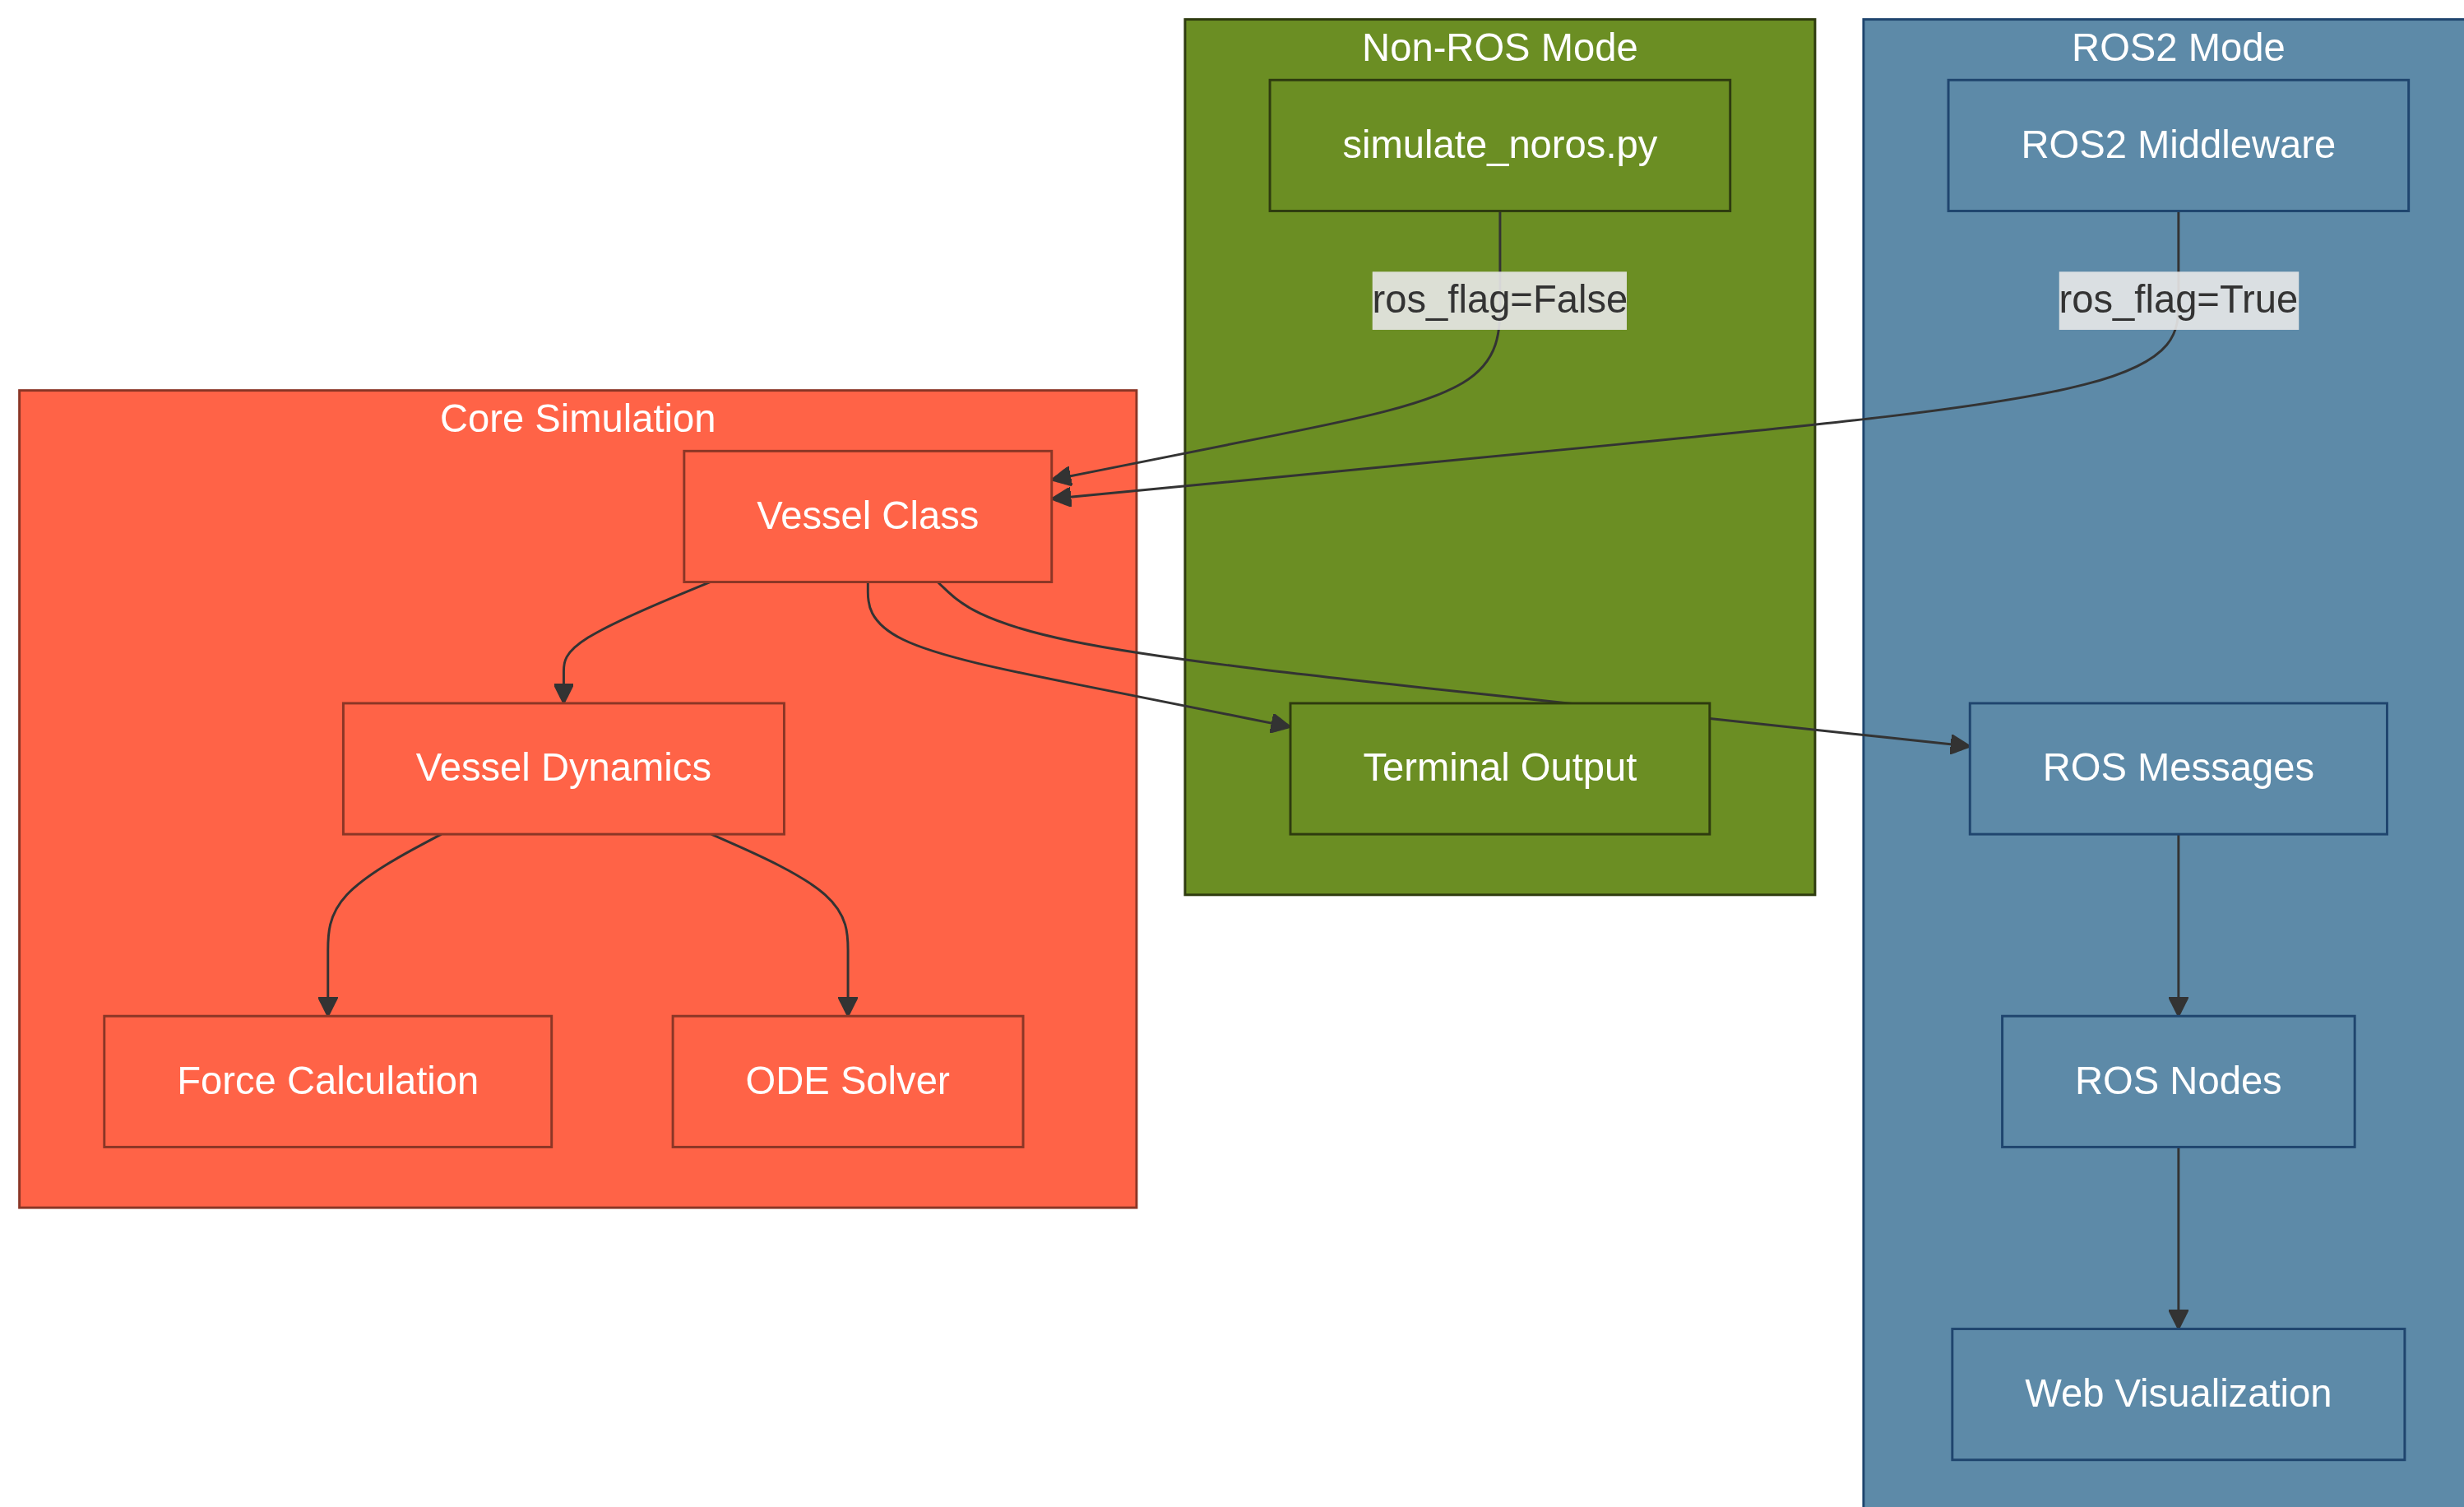
\includegraphics[width=10.8in,height=6.61in]{rawFiles/NoROS/noros_files/figure-latex/mermaid-figure-1.png}

\subsection*{\texorpdfstring{The \texttt{ros\_flag}
Parameter}{The ros\_flag Parameter}}\label{the-ros_flag-parameter}
\addcontentsline{toc}{subsection}{The \texttt{ros\_flag} Parameter}

The \texttt{ros\_flag} parameter in the \texttt{Vessel} class
constructor determines whether the vessel should use ROS2-specific
functionality:

\begin{Shaded}
\begin{Highlighting}[]
\KeywordTok{def} \FunctionTok{\_\_init\_\_}\NormalTok{(}\VariableTok{self}\NormalTok{, vessel\_params: Dict, hydrodynamic\_data: Dict, vessel\_id: }\BuiltInTok{int}\NormalTok{, ros\_flag: }\BuiltInTok{bool} \OperatorTok{=} \VariableTok{True}\NormalTok{):}
    \CommentTok{"""Initialize vessel with parameters and hydrodynamic data.}
\CommentTok{    }
\CommentTok{    Args:}
\CommentTok{        vessel\_params: Dictionary containing vessel parameters}
\CommentTok{        hydrodynamic\_data: Dictionary containing hydrodynamic coefficients}
\CommentTok{        vessel\_id: Unique identifier for the vessel}
\CommentTok{        ros\_flag: Flag indicating whether to use ROS2 functionality}
\CommentTok{    """}
    \VariableTok{self}\NormalTok{.ros\_flag }\OperatorTok{=}\NormalTok{ ros\_flag}
    \CommentTok{\# ... rest of initialization}
\end{Highlighting}
\end{Shaded}

When \texttt{ros\_flag} is set to \texttt{False}:

\begin{enumerate}
\def\labelenumi{\arabic{enumi}.}
\tightlist
\item
  No ROS2 node is created for the vessel
\item
  No publishers or subscribers are established
\item
  Command inputs must be set directly in code or through custom control
  logic
\item
  Simulation data is displayed in the terminal instead of through ROS2
  topics
\end{enumerate}

\section*{Running the Non-ROS
Simulator}\label{running-the-non-ros-simulator}
\addcontentsline{toc}{section}{Running the Non-ROS Simulator}

\markright{Running the Non-ROS Simulator}

To run Panisim without ROS2:

\begin{enumerate}
\def\labelenumi{\arabic{enumi}.}
\tightlist
\item
  Navigate to the makara directory
\item
  Run the \texttt{simulate\_noros.py} script:
\end{enumerate}

\begin{Shaded}
\begin{Highlighting}[]
\BuiltInTok{cd}\NormalTok{ /workspaces/mavlab/ros2\_ws/src/mav\_simulator/mav\_simulator}
\ExtensionTok{python3}\NormalTok{ simulate\_noros.py}
\end{Highlighting}
\end{Shaded}

The simulation will use the same configuration files as the ROS2
version, loading vessel parameters, hydrodynamics, and initial
conditions from the input files.

\subsection*{Simulation Output}\label{simulation-output}
\addcontentsline{toc}{subsection}{Simulation Output}

The non-ROS simulator provides detailed terminal output showing:

\begin{itemize}
\tightlist
\item
  Simulation time
\item
  Vessel position and orientation
\item
  Linear and angular velocities
\item
  Forces acting on the vessel, including:

  \begin{itemize}
  \tightlist
  \item
    Hydrodynamic forces
  \item
    Gravitational forces
  \item
    Control surface forces
  \item
    Thruster forces
  \end{itemize}
\item
  Control surface angles
\item
  Thruster RPMs
\end{itemize}

Example output:

\begin{verbatim}
Starting simulation...
Time [s] | Position [x, y, z] | Velocity [u, v, w]
------------------------------------------------------------

Time:   0.00
Position [x, y, z]: [  0.00,   0.00,   0.00]
Velocity [u, v, w]: [  0.50,   0.00,   0.00]
Orientation [phi, theta, psi] (deg): [  0.00,   0.00,   0.00]
Hydrodynamic forces: [ -0.40,   0.00,   0.00,   0.00,   0.00,   0.00]
Gravitational forces: [  0.00,   0.00,   0.00,   0.00,   0.00,   0.00]
Control surface forces: [  0.00,   0.00,   0.00,   0.00,   0.00,   0.00]
Thruster forces: [  0.00,   0.00,   0.00,   0.00,   0.00,   0.00]
Control surface angles [deg]: []
Thruster RPMs: []

Time:   0.01
Position [x, y, z]: [  0.01,   0.00,   0.00]
Velocity [u, v, w]: [  0.50,   0.00,   0.00]
...
\end{verbatim}

\section*{Implementing Custom
Controllers}\label{implementing-custom-controllers}
\addcontentsline{toc}{section}{Implementing Custom Controllers}

\markright{Implementing Custom Controllers}

One of the key advantages of the non-ROS mode is the ability to easily
implement custom controllers directly in the code. The
\texttt{vessel\_ode} method in \texttt{class\_vessel.py} contains a
section specifically for non-ROS mode:

\begin{Shaded}
\begin{Highlighting}[]
\ControlFlowTok{if} \KeywordTok{not} \VariableTok{self}\NormalTok{.ros\_flag:}
    \CommentTok{\#\# }\AlertTok{TODO}\CommentTok{: Implement your controller logic here to get the actuator commands}
    
    \CommentTok{\#\# example}
    \CommentTok{\# if self.control\_surface\_control\_type == \textquotesingle{}fixed\_rudder\textquotesingle{}:}
    \CommentTok{\#     self.delta\_c = con.fixed\_rudder(t, state, n\_control\_surfaces, 10.0) \#Enter rudder angle here}
    \CommentTok{\# elif self.control\_surface\_control\_type == \textquotesingle{}switching\_rudder\textquotesingle{}:}
    \CommentTok{\#     self.delta\_c = con.switching\_rudder(t, state, n\_control\_surfaces)}
    \CommentTok{\# else:}
    \CommentTok{\#     raise ValueError(f"Invalid control surface control type: \{self.control\_surface\_control\_type\}")}
        
    \CommentTok{\# \# Get thruster commands}
    \CommentTok{\# if self.thruster\_control\_type == \textquotesingle{}fixed\_rpm\textquotesingle{}:}
    \CommentTok{\#     self.n\_c = con.fixed\_thrust(t, state, n\_thrusters,1000.0) \#Enter RPM here}
    \CommentTok{\# else:}
    \CommentTok{\#     raise ValueError(f"Invalid thruster control type: \{self.thruster\_control\_type\}")}
    \ControlFlowTok{pass}
\end{Highlighting}
\end{Shaded}

To implement your own controller:

\begin{enumerate}
\def\labelenumi{\arabic{enumi}.}
\tightlist
\item
  Create a controller module (e.g., \texttt{my\_controller.py}) with
  your control algorithms
\item
  Import your controller module in \texttt{simulate\_noros.py}
\item
  Modify the \texttt{vessel\_ode} method to use your controller:
\end{enumerate}

\begin{Shaded}
\begin{Highlighting}[]
\CommentTok{\# In vessel\_ode method of class\_vessel.py}
\ControlFlowTok{if} \KeywordTok{not} \VariableTok{self}\NormalTok{.ros\_flag:}
    \CommentTok{\# Custom controller implementation}
    \ControlFlowTok{if} \BuiltInTok{hasattr}\NormalTok{(}\VariableTok{self}\NormalTok{, }\StringTok{\textquotesingle{}control\_surface\_control\_type\textquotesingle{}}\NormalTok{):}
        \ControlFlowTok{if} \VariableTok{self}\NormalTok{.control\_surface\_control\_type }\OperatorTok{==} \StringTok{\textquotesingle{}my\_controller\textquotesingle{}}\NormalTok{:}
            \VariableTok{self}\NormalTok{.delta\_c }\OperatorTok{=}\NormalTok{ my\_controller.calculate\_rudder(t, state, }\VariableTok{self}\NormalTok{.n\_control\_surfaces)}
\end{Highlighting}
\end{Shaded}

\subsection*{Example: Adding a Simple PID
Controller}\label{example-adding-a-simple-pid-controller}
\addcontentsline{toc}{subsection}{Example: Adding a Simple PID
Controller}

Here's an example of how to add a simple PID heading controller:

\begin{enumerate}
\def\labelenumi{\arabic{enumi}.}
\tightlist
\item
  Create a controller module:
\end{enumerate}

\begin{Shaded}
\begin{Highlighting}[]
\CommentTok{\# my\_controller.py}
\ImportTok{import}\NormalTok{ numpy }\ImportTok{as}\NormalTok{ np}

\KeywordTok{def}\NormalTok{ pid\_heading\_controller(t, state, n\_surfaces, desired\_heading}\OperatorTok{=}\FloatTok{0.0}\NormalTok{):}
    \CommentTok{"""Simple PID heading controller.}
\CommentTok{    }
\CommentTok{    Args:}
\CommentTok{        t: Current time}
\CommentTok{        state: Vessel state vector}
\CommentTok{        n\_surfaces: Number of control surfaces}
\CommentTok{        desired\_heading: Target heading in radians}
\CommentTok{        }
\CommentTok{    Returns:}
\CommentTok{        numpy.ndarray: Control surface angles in radians}
\CommentTok{    """}
    \CommentTok{\# Extract current heading}
\NormalTok{    current\_heading }\OperatorTok{=}\NormalTok{ state[}\DecValTok{11}\NormalTok{]  }\CommentTok{\# psi is at index 11}
    
    \CommentTok{\# Calculate heading error}
\NormalTok{    heading\_error }\OperatorTok{=}\NormalTok{ desired\_heading }\OperatorTok{{-}}\NormalTok{ current\_heading}
    
    \CommentTok{\# Normalize to {-}pi to pi}
\NormalTok{    heading\_error }\OperatorTok{=}\NormalTok{ (heading\_error }\OperatorTok{+}\NormalTok{ np.pi) }\OperatorTok{\%}\NormalTok{ (}\DecValTok{2} \OperatorTok{*}\NormalTok{ np.pi) }\OperatorTok{{-}}\NormalTok{ np.pi}
    
    \CommentTok{\# PID gains}
\NormalTok{    Kp }\OperatorTok{=} \FloatTok{0.5}
\NormalTok{    Ki }\OperatorTok{=} \FloatTok{0.01}
\NormalTok{    Kd }\OperatorTok{=} \FloatTok{0.1}
    
    \CommentTok{\# Calculate PID terms (simplified {-} would need integral and derivative state)}
\NormalTok{    p\_term }\OperatorTok{=}\NormalTok{ Kp }\OperatorTok{*}\NormalTok{ heading\_error}
    
    \CommentTok{\# Calculate rudder command (assume first surface is main rudder)}
\NormalTok{    rudder\_angle }\OperatorTok{=}\NormalTok{ np.clip(p\_term, }\OperatorTok{{-}}\NormalTok{np.pi}\OperatorTok{/}\DecValTok{4}\NormalTok{, np.pi}\OperatorTok{/}\DecValTok{4}\NormalTok{)}
    
    \CommentTok{\# Create control surface command array}
\NormalTok{    delta\_c }\OperatorTok{=}\NormalTok{ np.zeros(n\_surfaces)}
    \ControlFlowTok{if}\NormalTok{ n\_surfaces }\OperatorTok{\textgreater{}} \DecValTok{0}\NormalTok{:}
\NormalTok{        delta\_c[}\DecValTok{0}\NormalTok{] }\OperatorTok{=}\NormalTok{ rudder\_angle}
    
    \ControlFlowTok{return}\NormalTok{ delta\_c}
\end{Highlighting}
\end{Shaded}

\begin{enumerate}
\def\labelenumi{\arabic{enumi}.}
\setcounter{enumi}{1}
\tightlist
\item
  Modify the \texttt{vessel\_ode} method in \texttt{class\_vessel.py}:
\end{enumerate}

\begin{Shaded}
\begin{Highlighting}[]
\ControlFlowTok{if} \KeywordTok{not} \VariableTok{self}\NormalTok{.ros\_flag:}
    \CommentTok{\# Import controller at the top of the file}
    \ImportTok{import}\NormalTok{ my\_controller}
    
    \CommentTok{\# Use controller for rudder commands}
    \VariableTok{self}\NormalTok{.delta\_c }\OperatorTok{=}\NormalTok{ my\_controller.pid\_heading\_controller(}
\NormalTok{        t, state, }\VariableTok{self}\NormalTok{.n\_control\_surfaces, desired\_heading}\OperatorTok{=}\NormalTok{np.pi}\OperatorTok{/}\DecValTok{4}\NormalTok{)  }\CommentTok{\# 45 degrees}
    
    \CommentTok{\# Set thruster commands if needed}
    \ControlFlowTok{if} \VariableTok{self}\NormalTok{.n\_thrusters }\OperatorTok{\textgreater{}} \DecValTok{0}\NormalTok{:}
        \VariableTok{self}\NormalTok{.n\_c }\OperatorTok{=}\NormalTok{ np.ones(}\VariableTok{self}\NormalTok{.n\_thrusters) }\OperatorTok{*} \FloatTok{1000.0}  \CommentTok{\# Fixed RPM}
\end{Highlighting}
\end{Shaded}

\section*{Customizing the Non-ROS
Simulator}\label{customizing-the-non-ros-simulator}
\addcontentsline{toc}{section}{Customizing the Non-ROS Simulator}

\markright{Customizing the Non-ROS Simulator}

\subsection*{Modifying Simulation
Parameters}\label{modifying-simulation-parameters}
\addcontentsline{toc}{subsection}{Modifying Simulation Parameters}

You can customize the simulation by modifying the
\texttt{simulate\_noros.py} file:

\begin{enumerate}
\def\labelenumi{\arabic{enumi}.}
\item
  \textbf{Change input file path}:

\begin{Shaded}
\begin{Highlighting}[]
\NormalTok{sim\_params, agents }\OperatorTok{=}\NormalTok{ read\_input(}\StringTok{"/path/to/your/custom\_input.yml"}\NormalTok{)}
\end{Highlighting}
\end{Shaded}
\item
  \textbf{Modify output format}:

\begin{Shaded}
\begin{Highlighting}[]
\CommentTok{\# Customize the print statements in the simulation loop}
\BuiltInTok{print}\NormalTok{(}\SpecialStringTok{f"Custom format: time=}\SpecialCharTok{\{}\NormalTok{vessel}\SpecialCharTok{.}\NormalTok{t}\SpecialCharTok{:6.2f\}}\SpecialStringTok{, position=[}\SpecialCharTok{\{}\NormalTok{pos[}\DecValTok{0}\NormalTok{]}\SpecialCharTok{:6.2f\}}\SpecialStringTok{, }\SpecialCharTok{\{}\NormalTok{pos[}\DecValTok{1}\NormalTok{]}\SpecialCharTok{:6.2f\}}\SpecialStringTok{]"}\NormalTok{)}
\end{Highlighting}
\end{Shaded}
\item
  \textbf{Add data logging}:

\begin{Shaded}
\begin{Highlighting}[]
\CommentTok{\# Add at the beginning of the simulate function}
\ImportTok{import}\NormalTok{ csv}
\NormalTok{log\_file }\OperatorTok{=} \BuiltInTok{open}\NormalTok{(}\StringTok{\textquotesingle{}simulation\_log.csv\textquotesingle{}}\NormalTok{, }\StringTok{\textquotesingle{}w\textquotesingle{}}\NormalTok{, newline}\OperatorTok{=}\StringTok{\textquotesingle{}\textquotesingle{}}\NormalTok{)}
\NormalTok{csv\_writer }\OperatorTok{=}\NormalTok{ csv.writer(log\_file)}
\NormalTok{csv\_writer.writerow([}\StringTok{\textquotesingle{}Time\textquotesingle{}}\NormalTok{, }\StringTok{\textquotesingle{}X\textquotesingle{}}\NormalTok{, }\StringTok{\textquotesingle{}Y\textquotesingle{}}\NormalTok{, }\StringTok{\textquotesingle{}Z\textquotesingle{}}\NormalTok{, }\StringTok{\textquotesingle{}U\textquotesingle{}}\NormalTok{, }\StringTok{\textquotesingle{}V\textquotesingle{}}\NormalTok{, }\StringTok{\textquotesingle{}W\textquotesingle{}}\NormalTok{, }\StringTok{\textquotesingle{}P\textquotesingle{}}\NormalTok{, }\StringTok{\textquotesingle{}Q\textquotesingle{}}\NormalTok{, }\StringTok{\textquotesingle{}R\textquotesingle{}}\NormalTok{, }\StringTok{\textquotesingle{}Phi\textquotesingle{}}\NormalTok{, }\StringTok{\textquotesingle{}Theta\textquotesingle{}}\NormalTok{, }\StringTok{\textquotesingle{}Psi\textquotesingle{}}\NormalTok{])}

\CommentTok{\# Inside the simulation loop}
\NormalTok{csv\_writer.writerow([vessel.t, pos[}\DecValTok{0}\NormalTok{], pos[}\DecValTok{1}\NormalTok{], pos[}\DecValTok{2}\NormalTok{], vel[}\DecValTok{0}\NormalTok{], vel[}\DecValTok{1}\NormalTok{], vel[}\DecValTok{2}\NormalTok{], }
\NormalTok{                    vessel.current\_state[}\DecValTok{3}\NormalTok{], vessel.current\_state[}\DecValTok{4}\NormalTok{], vessel.current\_state[}\DecValTok{5}\NormalTok{],}
\NormalTok{                    angles[}\DecValTok{0}\NormalTok{], angles[}\DecValTok{1}\NormalTok{], angles[}\DecValTok{2}\NormalTok{]])}
\end{Highlighting}
\end{Shaded}
\end{enumerate}

\subsection*{Extending the Simulator}\label{extending-the-simulator}
\addcontentsline{toc}{subsection}{Extending the Simulator}

You can extend the non-ROS simulator for specific use cases:

\begin{enumerate}
\def\labelenumi{\arabic{enumi}.}
\item
  \textbf{Batch simulations}:

\begin{Shaded}
\begin{Highlighting}[]
\KeywordTok{def}\NormalTok{ run\_batch\_simulations():}
\NormalTok{    results }\OperatorTok{=}\NormalTok{ []}
    \ControlFlowTok{for}\NormalTok{ initial\_speed }\KeywordTok{in}\NormalTok{ [}\FloatTok{0.5}\NormalTok{, }\FloatTok{1.0}\NormalTok{, }\FloatTok{1.5}\NormalTok{, }\FloatTok{2.0}\NormalTok{]:}
\NormalTok{        sim\_params, agents }\OperatorTok{=}\NormalTok{ read\_input(}\StringTok{"/workspaces/mavlab/inputs/simulation\_input.yml"}\NormalTok{)}
\NormalTok{        agents[}\DecValTok{0}\NormalTok{][}\StringTok{\textquotesingle{}vessel\_config\textquotesingle{}}\NormalTok{][}\StringTok{\textquotesingle{}initial\_conditions\textquotesingle{}}\NormalTok{][}\StringTok{\textquotesingle{}start\_velocity\textquotesingle{}}\NormalTok{][}\DecValTok{0}\NormalTok{] }\OperatorTok{=}\NormalTok{ initial\_speed}
\NormalTok{        vessel }\OperatorTok{=}\NormalTok{ Vessel(agents[}\DecValTok{0}\NormalTok{][}\StringTok{\textquotesingle{}vessel\_config\textquotesingle{}}\NormalTok{], agents[}\DecValTok{0}\NormalTok{][}\StringTok{\textquotesingle{}hydrodynamics\textquotesingle{}}\NormalTok{], vessel\_id}\OperatorTok{=}\DecValTok{0}\NormalTok{, ros\_flag}\OperatorTok{=}\VariableTok{False}\NormalTok{)}
\NormalTok{        vessel.simulate()}
        \CommentTok{\# Extract results}
\NormalTok{        final\_pos }\OperatorTok{=}\NormalTok{ vessel.history[}\OperatorTok{{-}}\DecValTok{1}\NormalTok{, }\DecValTok{6}\NormalTok{:}\DecValTok{9}\NormalTok{]}
\NormalTok{        results.append((initial\_speed, final\_pos))}
    \ControlFlowTok{return}\NormalTok{ results}
\end{Highlighting}
\end{Shaded}
\item
  \textbf{Parameter studies}:

\begin{Shaded}
\begin{Highlighting}[]
\KeywordTok{def}\NormalTok{ parameter\_study():}
    \ImportTok{import}\NormalTok{ matplotlib.pyplot }\ImportTok{as}\NormalTok{ plt}

\NormalTok{    turning\_radii }\OperatorTok{=}\NormalTok{ []}
\NormalTok{    rudder\_angles }\OperatorTok{=}\NormalTok{ np.arange(}\OperatorTok{{-}}\DecValTok{30}\NormalTok{, }\DecValTok{31}\NormalTok{, }\DecValTok{5}\NormalTok{) }\OperatorTok{*}\NormalTok{ np.pi }\OperatorTok{/} \DecValTok{180}  \CommentTok{\# {-}30 to 30 degrees}

    \ControlFlowTok{for}\NormalTok{ rudder\_angle }\KeywordTok{in}\NormalTok{ rudder\_angles:}
        \CommentTok{\# Set up simulation with fixed rudder angle}
\NormalTok{        sim\_params, agents }\OperatorTok{=}\NormalTok{ read\_input(}\StringTok{"/workspaces/mavlab/inputs/simulation\_input.yml"}\NormalTok{)}
\NormalTok{        vessel }\OperatorTok{=}\NormalTok{ Vessel(agents[}\DecValTok{0}\NormalTok{][}\StringTok{\textquotesingle{}vessel\_config\textquotesingle{}}\NormalTok{], agents[}\DecValTok{0}\NormalTok{][}\StringTok{\textquotesingle{}hydrodynamics\textquotesingle{}}\NormalTok{], vessel\_id}\OperatorTok{=}\DecValTok{0}\NormalTok{, ros\_flag}\OperatorTok{=}\VariableTok{False}\NormalTok{)}

        \CommentTok{\# Custom controller for fixed rudder}
\NormalTok{        vessel.control\_surface\_control\_type }\OperatorTok{=} \StringTok{\textquotesingle{}fixed\textquotesingle{}}
\NormalTok{        vessel.fixed\_rudder\_angle }\OperatorTok{=}\NormalTok{ rudder\_angle}

        \CommentTok{\# Run simulation}
\NormalTok{        vessel.simulate()}

        \CommentTok{\# Calculate turning radius from final path}
        \CommentTok{\# (simplified {-} would need actual path analysis)}
\NormalTok{        path }\OperatorTok{=}\NormalTok{ vessel.history[:, }\DecValTok{6}\NormalTok{:}\DecValTok{8}\NormalTok{]  }\CommentTok{\# x, y positions}
\NormalTok{        turning\_radius }\OperatorTok{=}\NormalTok{ calculate\_turning\_radius(path)}
\NormalTok{        turning\_radii.append(turning\_radius)}

    \CommentTok{\# Plot results}
\NormalTok{    plt.plot(rudder\_angles }\OperatorTok{*} \DecValTok{180} \OperatorTok{/}\NormalTok{ np.pi, turning\_radii)}
\NormalTok{    plt.xlabel(}\StringTok{\textquotesingle{}Rudder Angle (degrees)\textquotesingle{}}\NormalTok{)}
\NormalTok{    plt.ylabel(}\StringTok{\textquotesingle{}Turning Radius (m)\textquotesingle{}}\NormalTok{)}
\NormalTok{    plt.savefig(}\StringTok{\textquotesingle{}turning\_radius\_study.png\textquotesingle{}}\NormalTok{)}
\end{Highlighting}
\end{Shaded}
\end{enumerate}

\section*{Advantages of Non-ROS Mode}\label{advantages-of-non-ros-mode}
\addcontentsline{toc}{section}{Advantages of Non-ROS Mode}

\markright{Advantages of Non-ROS Mode}

The non-ROS mode offers several advantages:

\begin{enumerate}
\def\labelenumi{\arabic{enumi}.}
\tightlist
\item
  \textbf{Simplicity}: No need to set up ROS2 environment or handle
  ROS-specific configurations
\item
  \textbf{Performance}: Lower overhead without ROS middleware,
  especially for rapid prototyping
\item
  \textbf{Debugging}: Easier to debug core simulation components without
  ROS complexity
\item
  \textbf{Quick Testing}: Fast iteration for testing vessel dynamics or
  controller concepts
\item
  \textbf{Portability}: Can run anywhere Python is available, without
  ROS2 installation
\item
  \textbf{Learning}: Excellent starting point for understanding vessel
  dynamics before moving to ROS2
\item
  \textbf{Batch Processing}: Efficient for running multiple simulations
  for parameter studies or optimization
\end{enumerate}

\section*{Limitations}\label{limitations}
\addcontentsline{toc}{section}{Limitations}

\markright{Limitations}

Compared to the ROS2 mode, the non-ROS mode has some limitations:

\begin{enumerate}
\def\labelenumi{\arabic{enumi}.}
\tightlist
\item
  \textbf{No Visualization}: Lacks the web-based visualization dashboard
  available in ROS2 mode
\item
  \textbf{Limited External Interaction}: No standardized way to interact
  with external systems
\item
  \textbf{No Distributed Simulation}: Cannot distribute components
  across multiple processes/machines
\item
  \textbf{No Standardized Messaging}: No access to ROS2's message types
  and communication patterns
\item
  \textbf{Manual Data Collection}: Requires custom code for data logging
  and analysis
\end{enumerate}

\section*{Conclusion}\label{conclusion-1}
\addcontentsline{toc}{section}{Conclusion}

\markright{Conclusion}

The non-ROS mode provides a lightweight alternative for running Panisim
simulations without the complexity of the ROS2 ecosystem. It's
particularly useful for rapid development, testing, and educational
purposes. By understanding the implementation through \texttt{ros\_flag}
and custom controller integration, users can leverage this mode for a
wide range of applications while still benefiting from Panisim's
accurate vessel dynamics modeling.




\end{document}
